\chapter{Resultados obtenidos}
	\label{sec:resultados}

	En este capítulo se muestran pruebas realizadas a la implementación del RNA y el ACG en nueve diferentes casos de aplicación, que denominaremos \textit{ejemplos}. Estos ejemplos abarcan sistemas simples y complejos, desde ejemplos provistos por railML.org hasta sistemas reales, pasando por locaciones generadas artificialmente por el autor de este trabajo para probar cada una de las funcionalidades del RNA y del ACG. En las siguientes secciones se analizará en detalle el primer ejemplo, lo que es suficiente para que el lector entienda el flujo de trabajo y los resultados obtenidos. Los ocho ejemplos restantes se encuentran en apéndices.
	
	En cada uno de los ejemplos se comparará el señalamiento obtenido mediante RNA, con el señalamiento de referencia para ese ejemplo. De esta forma será posible obtener conclusiones respecto a la eficacia del RNA, su impacto en la logística, seguridad y cobertura de la red. El análisis incluye la presentación de la topología original junto con su señalamiento y tabla de enclavamientos, siempre que esté disponible. Adicionalmente, se ilustrará la generación paso a paso del señalamiento, su simplificación y tabla de enclavamientos final, junto con la comparación con el enclavamiento original, si existiese. Finalmente, se incluyen las redes de grafos generadas por el RNA y un resumen de los recursos utilizados por el ACG para implementar el sistema.
	
	Alguno de los ejemplos que se usarán para probar los algoritmos fueron tomados de railML.Org u otras fuentes y se hará referencia a ellos como "ejemplos tomados de railML", o bien se hará referencia a la fuente que corresponda, mientras que otros ejemplos que se usarán para probar los algoritmos fueron diseñados por el autor de esta tesis, y se hará referencia a ellos como "ejemplos diseñados para las pruebas". Cuando para el análisis se tome el señalamiento, sea el disponible en railML.Org o el diseñado por el autor, previo a ser procesador por el RNA se hablará de "señalamiento original", en el sentido de que se lo describirá previo a su procesamiento. En cambio, cuando para el análisis se tome el señalamiento producto de ser procesado por el RNA, se hablará de "señalamiento generado", ya que fue generado automáticamente por el RNA en base a la topología de la red ferroviaria.	
	
	\section{Plataforma utilizada}
	\label{sec:ARTY}
	
	Cómo se explicó Sección \ref{sec:plataforma}, es posible utilizar una FPGA de cualquier fabricante, siempre y cuando tenga determinadas características de tamaño. En este contexto se optó por utilizar la FPGA ARTY Z7-20 de Xilinx (Figura \ref{fig:FPGA}) debido a cuestiones de disponibilidad y experiencia previa con la plataforma. La misma posee 53200 Look-up-tables, 106400 Flip-Flops, 32 Buffers y 125 bloque de entrada/salida. El precio promedio de esta plataforma ronda los 300 U\$D, un precio razonable para una plataforma de nivel intermedio.	
	
	\begin{figure}[H]
		\centering
		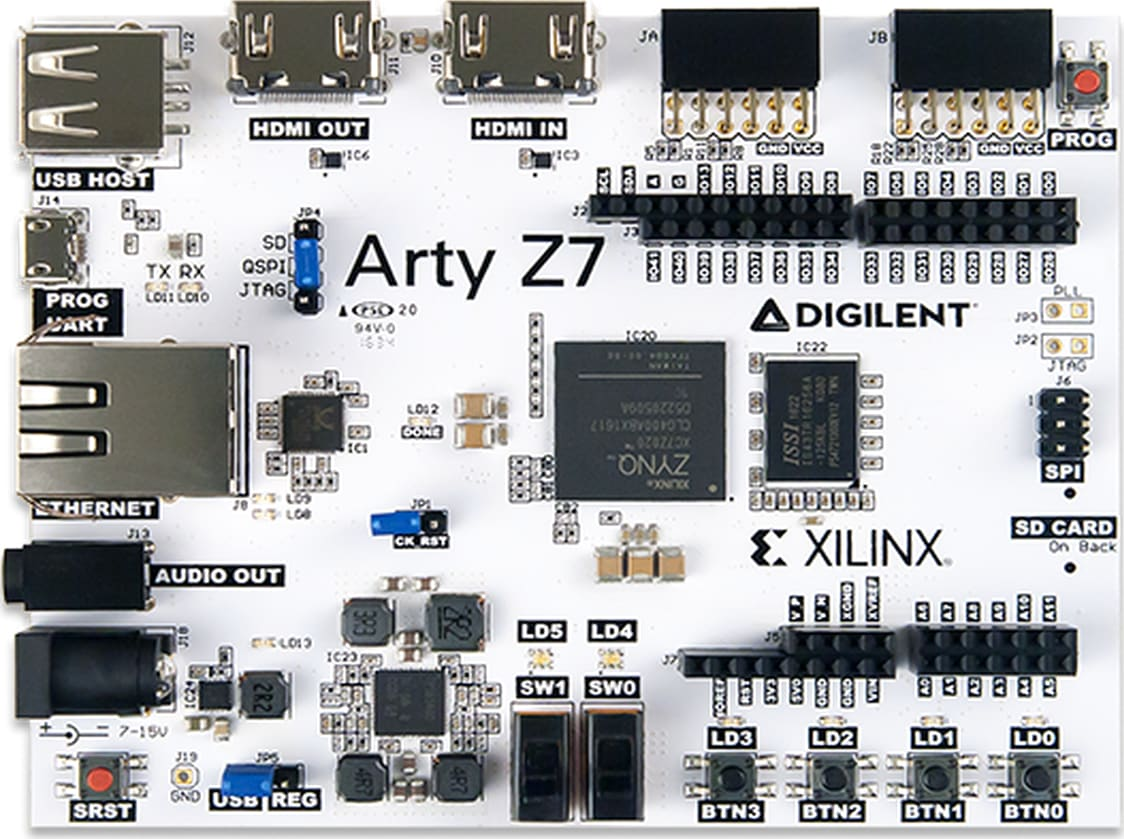
\includegraphics[width=1\textwidth]{Figuras/FPGA}
		\centering\caption{Plataforma FPGA Xilinx Arty Z7-20.}
		\label{fig:FPGA}
	\end{figure}
	
	Aunque se seleccionó una FPGA de la familia Xilinx \cite{Paper_30,Paper_36,Paper_37,Paper_40,Paper_41,Paper_47,Paper_97,Paper_104,Paper_106} y se utilizó el entorno de desarrollo integrado Vivado \cite{VIVADO,Paper_111}, por lo explicado en la Sección \ref{sec:plataforma}, el código VHDL generado por el ACG es independiente de la plataforma que se utilice. De emplearse otra familia de FPGAs, solo será necesaria una nueva asignación manual de pines de entrada y salida. De emplearse FPGAs por fuera de las familias ofrecidas por Xilinx, cómo por ejemplo Intel, puede utilizarse el entorno de desarrollo correspondiente, como por ejemplo el entorno de desarrollo Intel Quartus \cite{QUARTUS}.
	
	Tanto el entorno de desarrollo Xilinx Vivado como el Intel Quartus incorporan herramientas para validación de la sintaxis generada por el ACG. Se utilizó Xilinx Vivado para generar el diagrama de bloques del sistema y analizar cada uno de los módulos y sus elementos internos. Este proceso incluye una validación de la sintaxis de todos los archivos generados por el ACG. Un análisis similar se realiza en las etapas de síntesis e implementación, detallado en profundidad en este capítulo.
	
	%La elección de una FPGA por sobre un microprocesador se debe a las ventajas expuestas en la Sección \ref{sec:FPGA} respecto a la concurrencia del sistema, mayor nivel de seguridad y facilidad para redundar el sistema. Además, los sistemas implementados en FPGA son considerados puramente hardware y no software, por lo que solamente deben cumplir los requerimientos de la norma EN 50129, especialmente el anexo F referido a FPGAs, y no la norma EN 50128 que se encarga del software. Los alcances de estas normas ya fueron explicados en la Sección \ref{sec:normas}.
	
	\section{Ejemplo 1}

    \lipsum[1]

    \begin{figure}[h]
        \centering
        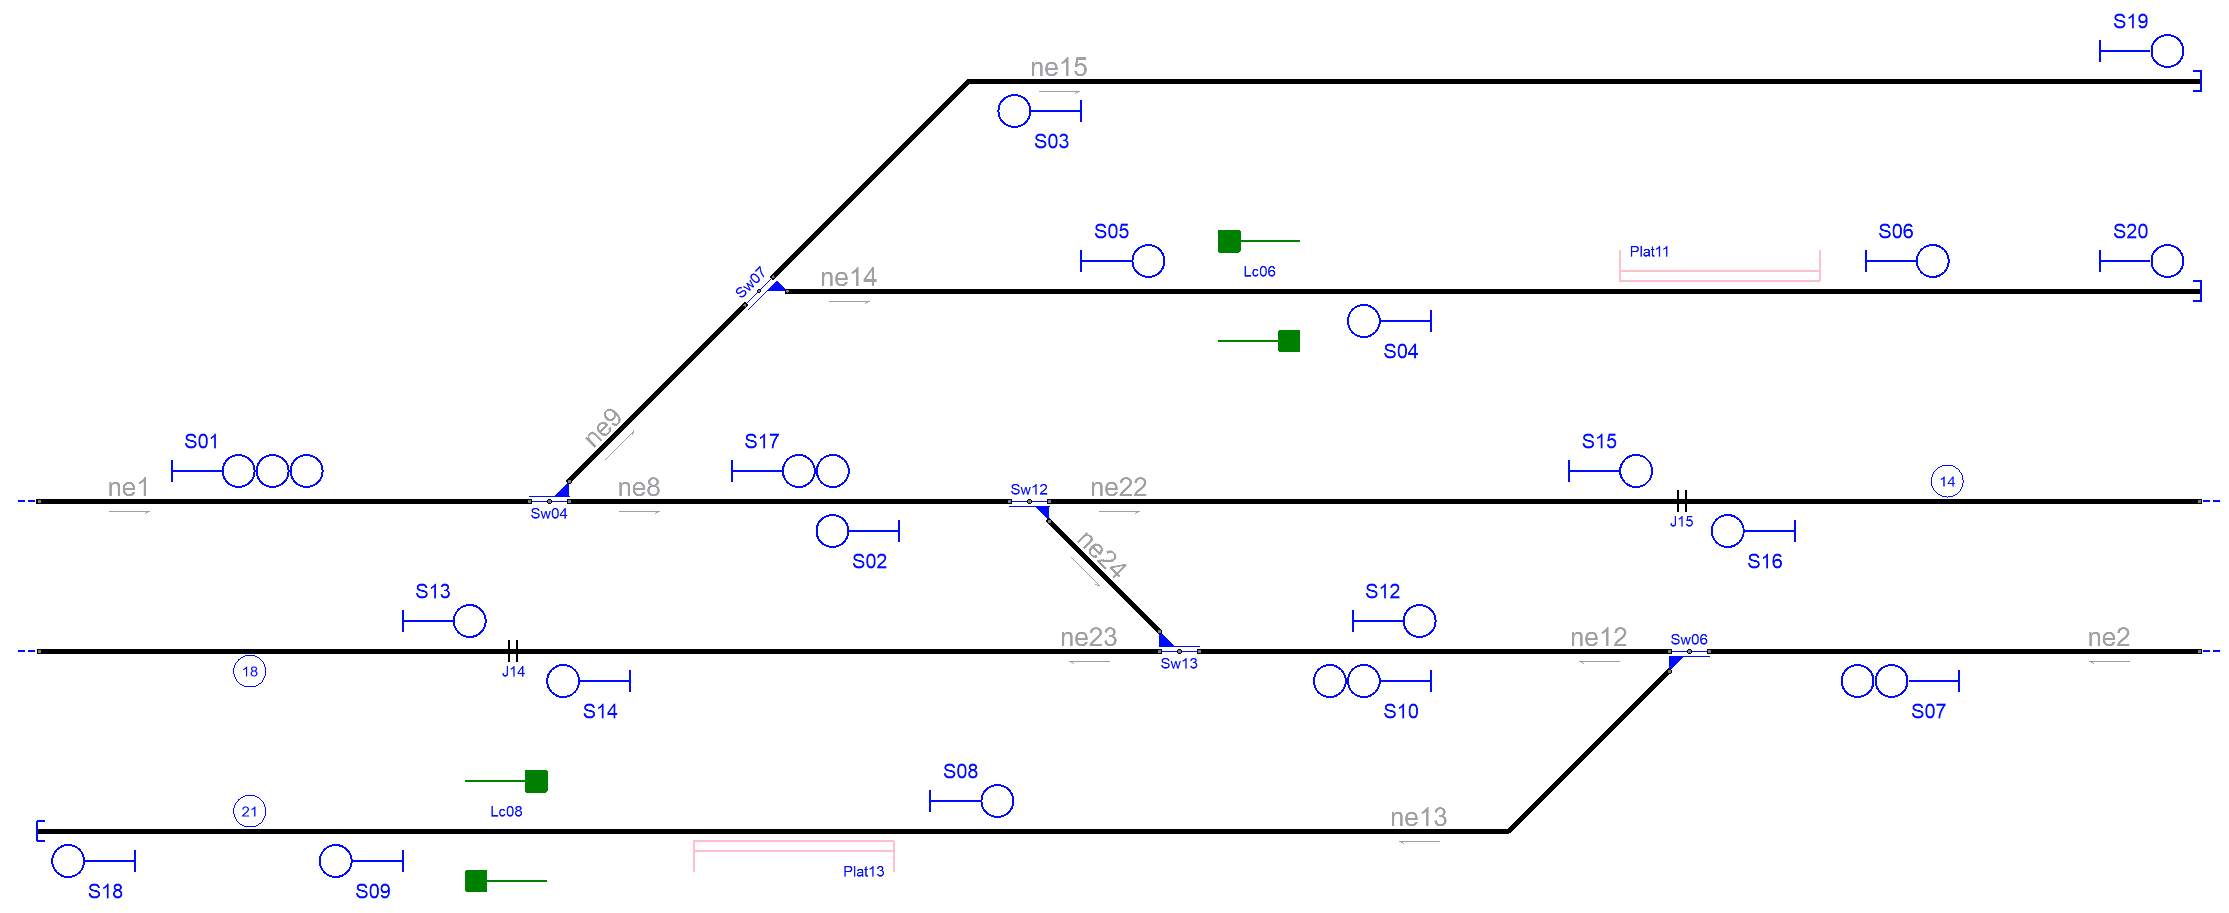
\includegraphics[width=1\textwidth]{resultados-obtenidos/ejemplo1/images/1_original.png}
        \centering\caption{Señalamiento original del ejemplo 1.}
        %\label{fig:LC_P2}
    \end{figure}

    \begin{figure}[h]
        \centering
        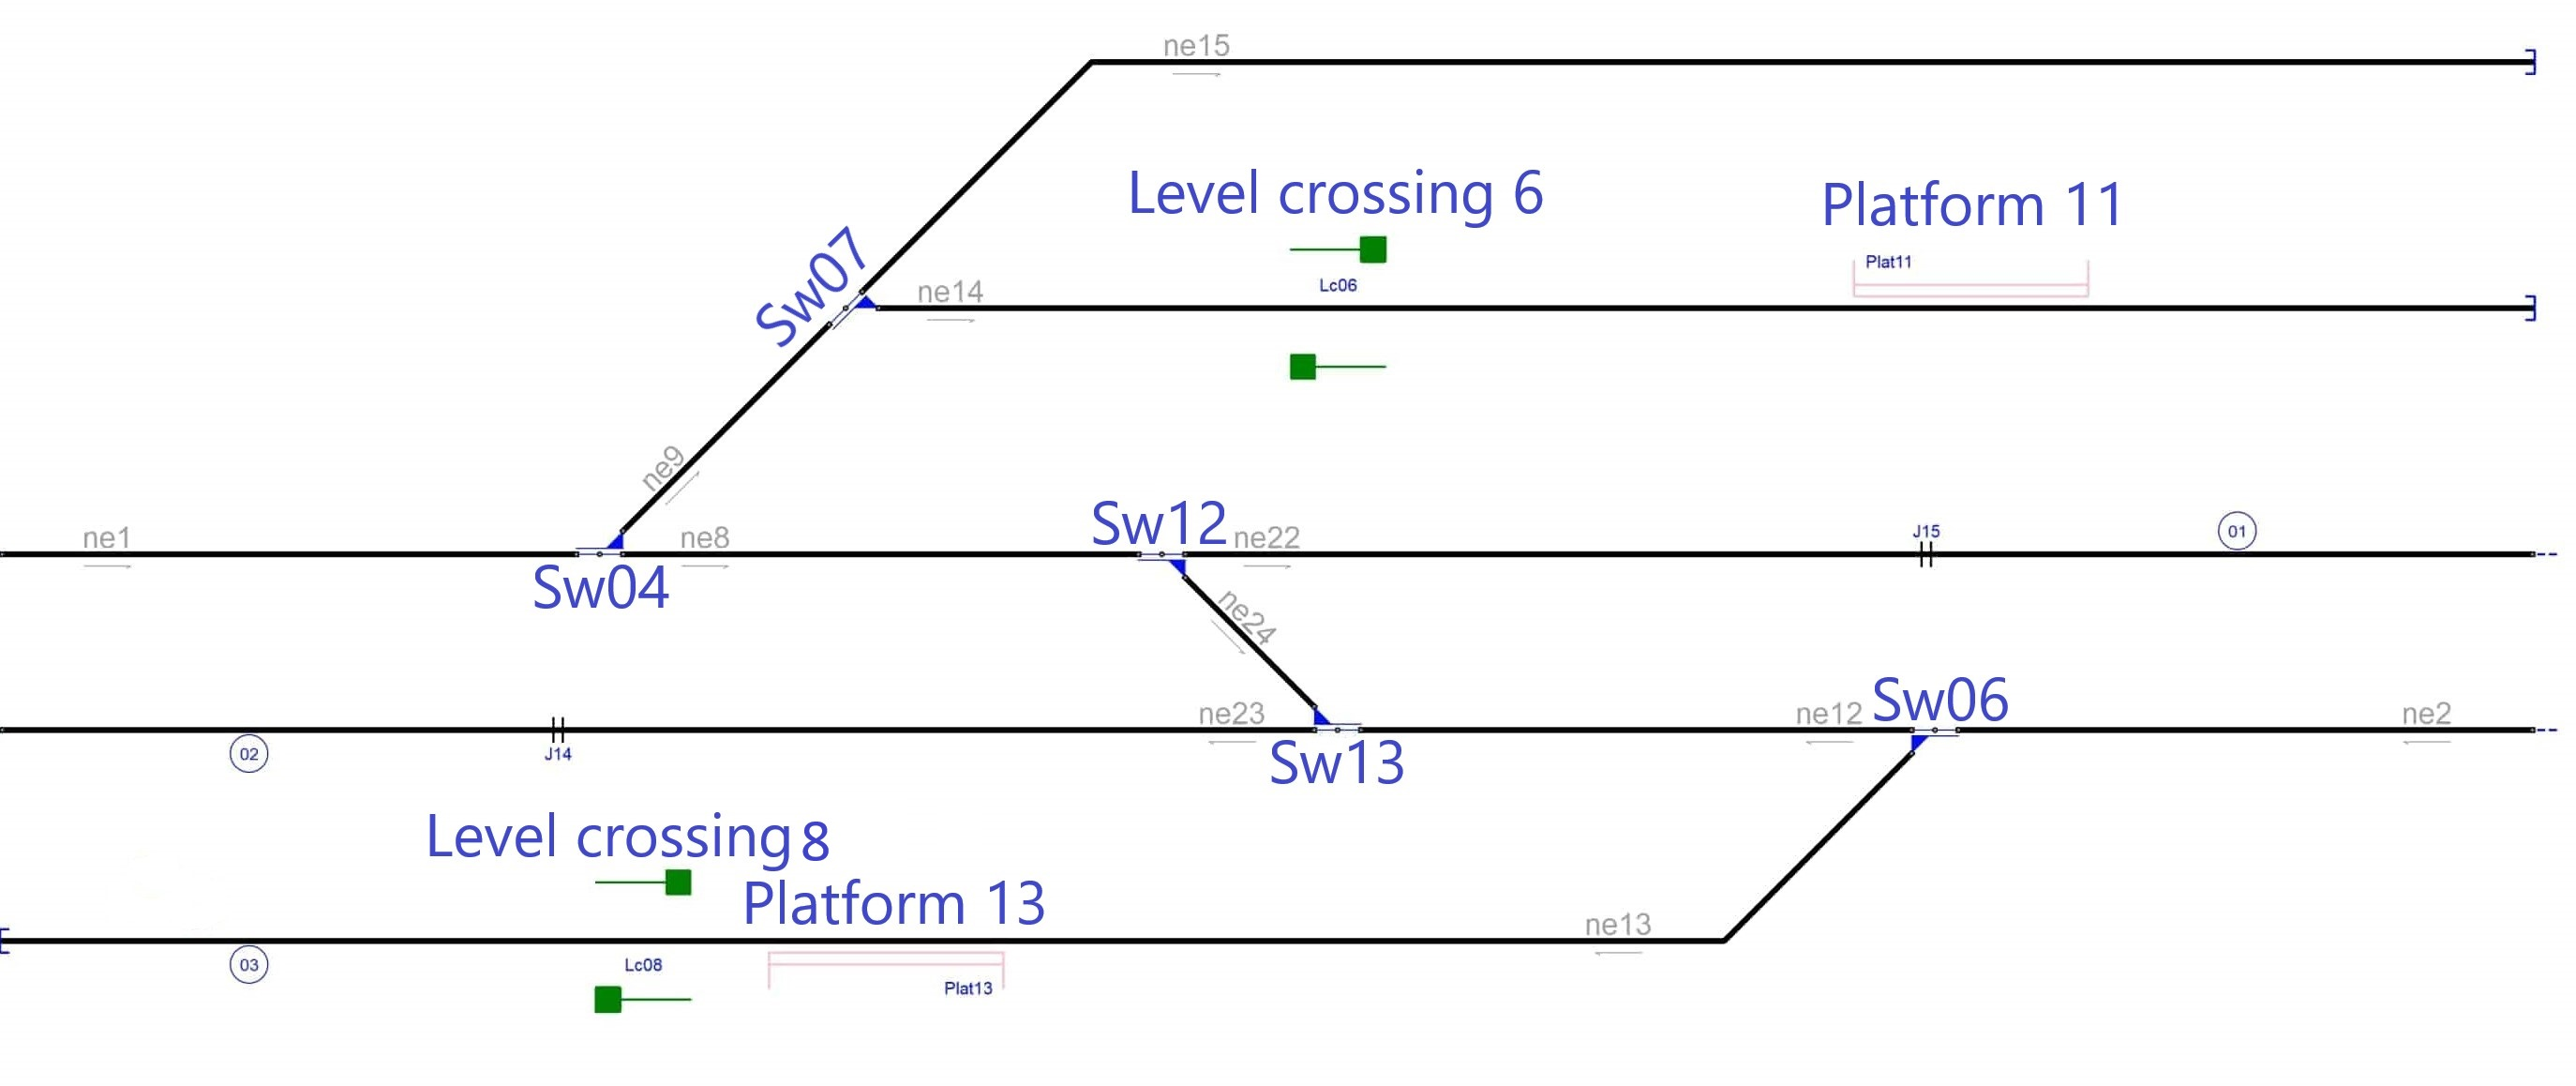
\includegraphics[width=1\textwidth]{resultados-obtenidos/ejemplo1/images/1_empty.png}
        \centering\caption{Topología ferroviaria del ejemplo 1 sin señalamiento.}
        %\label{fig:LC_P2}
    \end{figure}

    \begin{figure}[h]
        \centering
        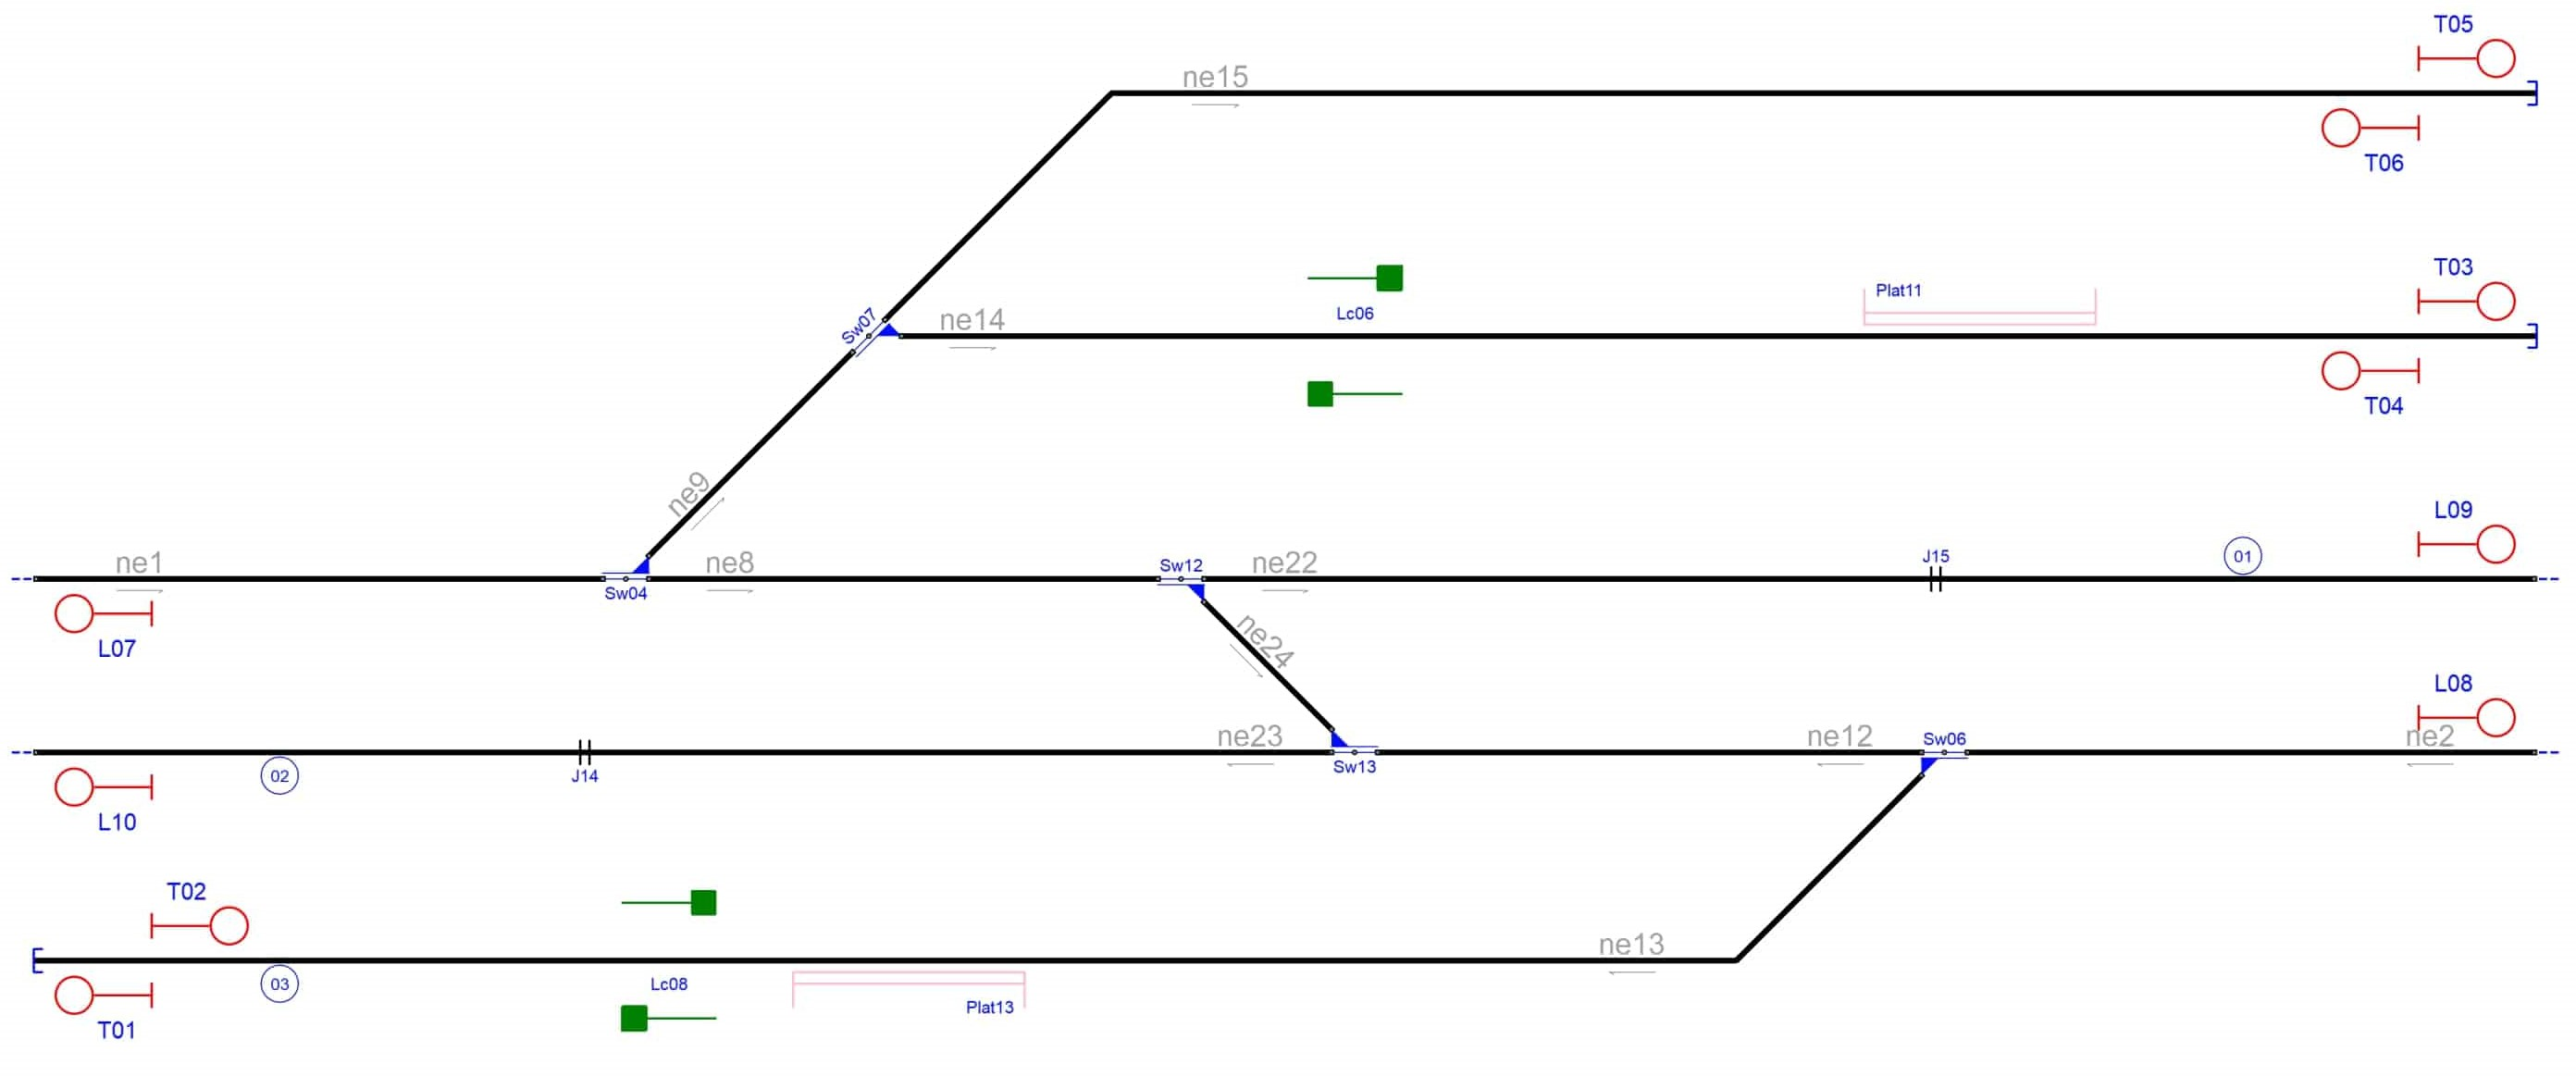
\includegraphics[width=1\textwidth]{resultados-obtenidos/ejemplo1/images/1_step1.png}
        \centering\caption{Señalamiento generado por el RNA para proteger el fín de vía.}
        %\label{fig:LC_P2}
    \end{figure}

    \begin{figure}[h]
        \centering
        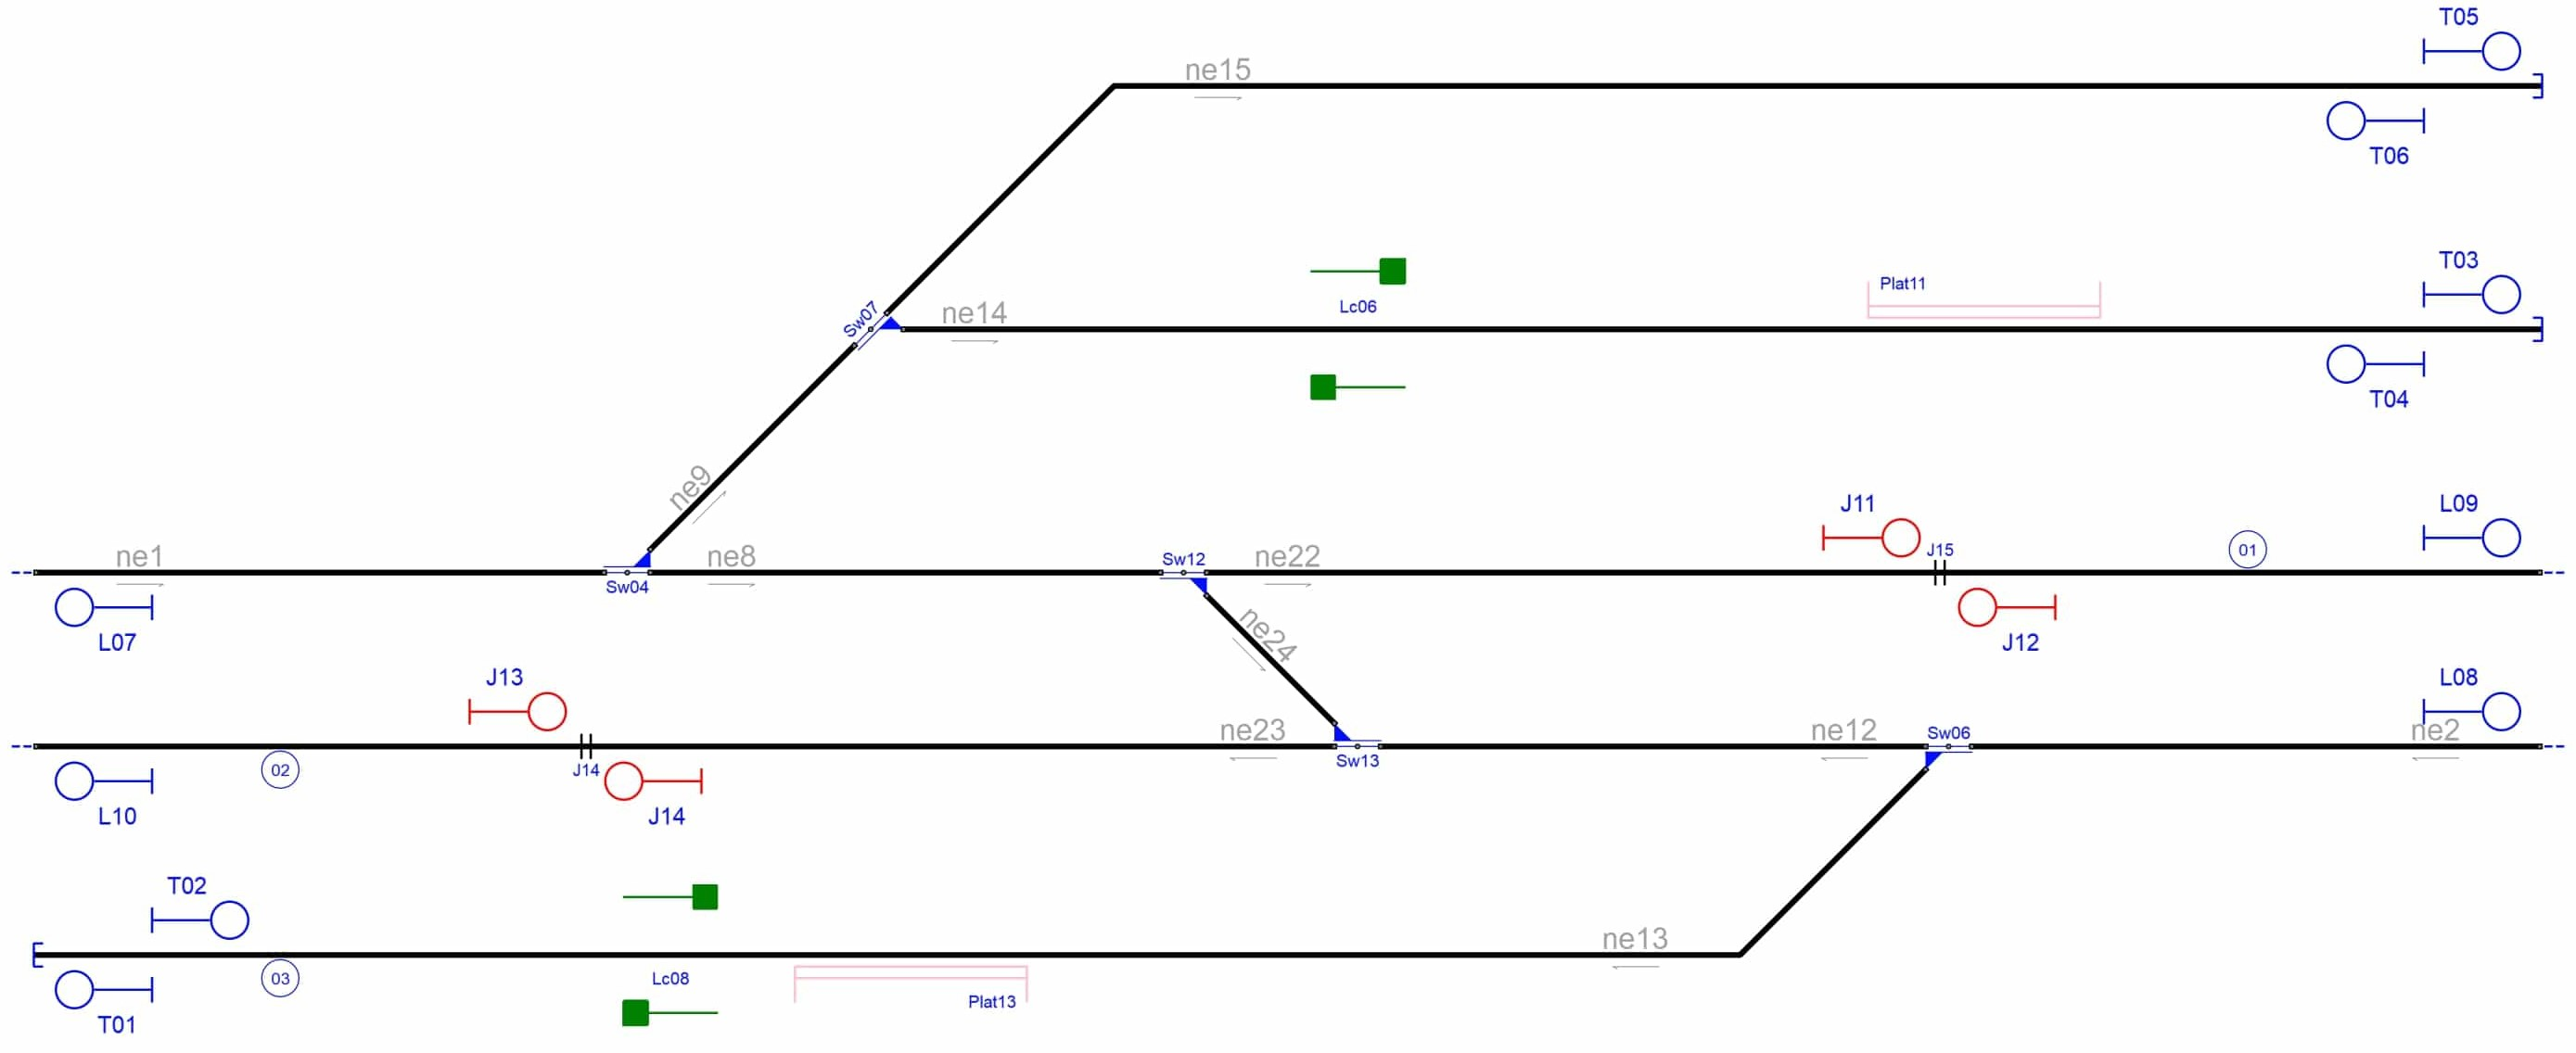
\includegraphics[width=1\textwidth]{resultados-obtenidos/ejemplo1/images/1_step2.png}
        \centering\caption{Señalamiento generado por el RNA para proteger las junturas.}
        %\label{fig:LC_P2}
    \end{figure}

    \begin{figure}[h]
        \centering
        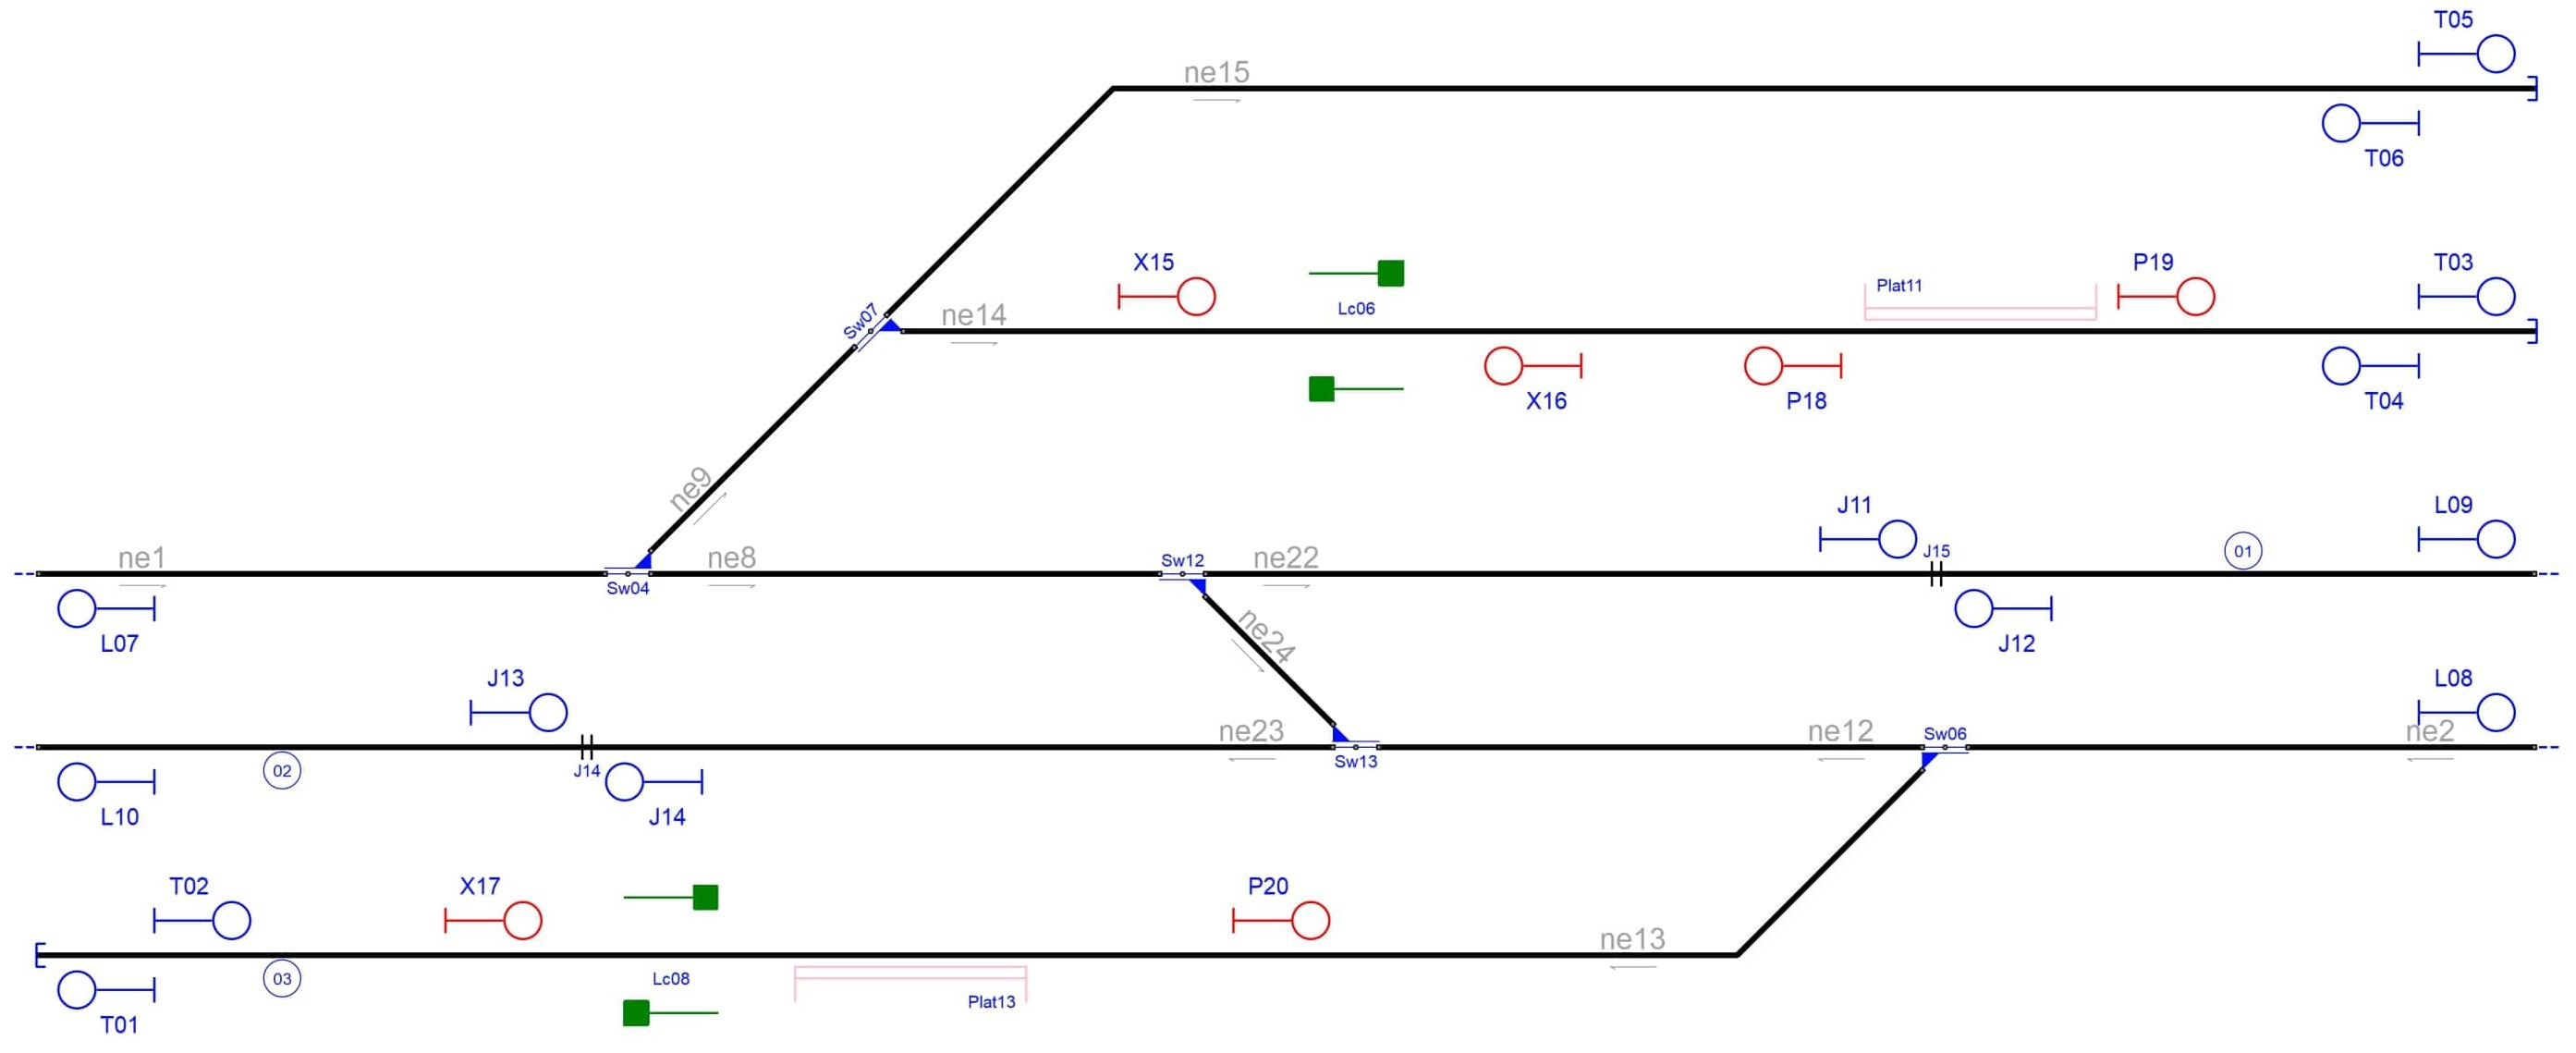
\includegraphics[width=1\textwidth]{resultados-obtenidos/ejemplo1/images/1_step3.png}
        \centering\caption{Señalamiento generado por el RNA para proteger plataformas y cruces de vía.}
        %\label{fig:LC_P2}
    \end{figure}

    \begin{figure}[h]
        \centering
        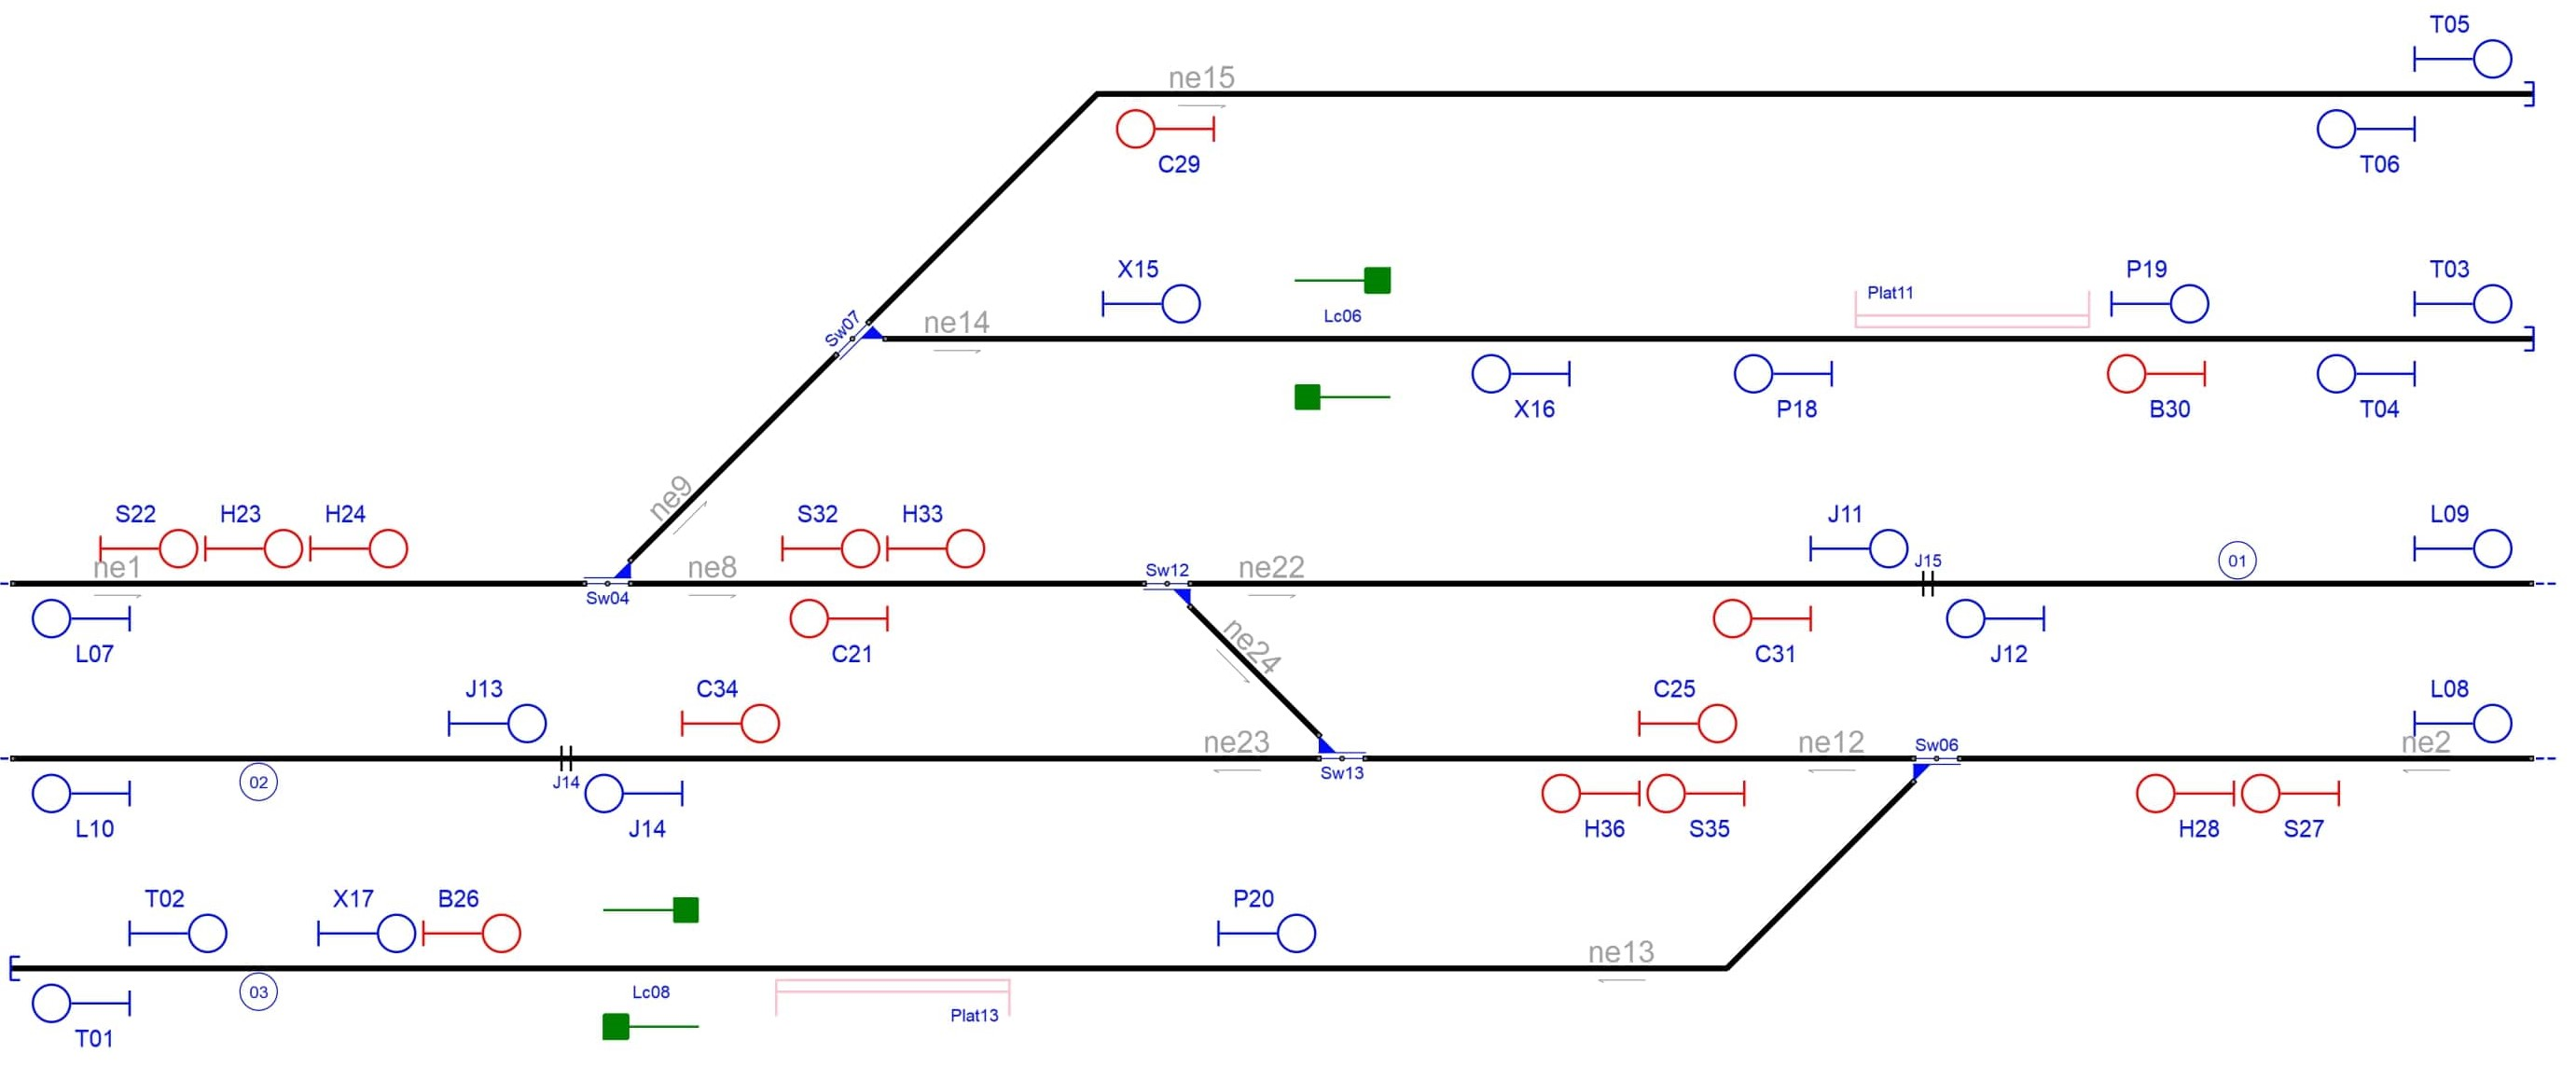
\includegraphics[width=1\textwidth]{resultados-obtenidos/ejemplo1/images/1_step4.png}
        \centering\caption{Señalamiento generado por el RNA para proteger las máquinas de cambios.}
        %\label{fig:LC_P2}
    \end{figure}

    \begin{figure}[h]
        \centering
        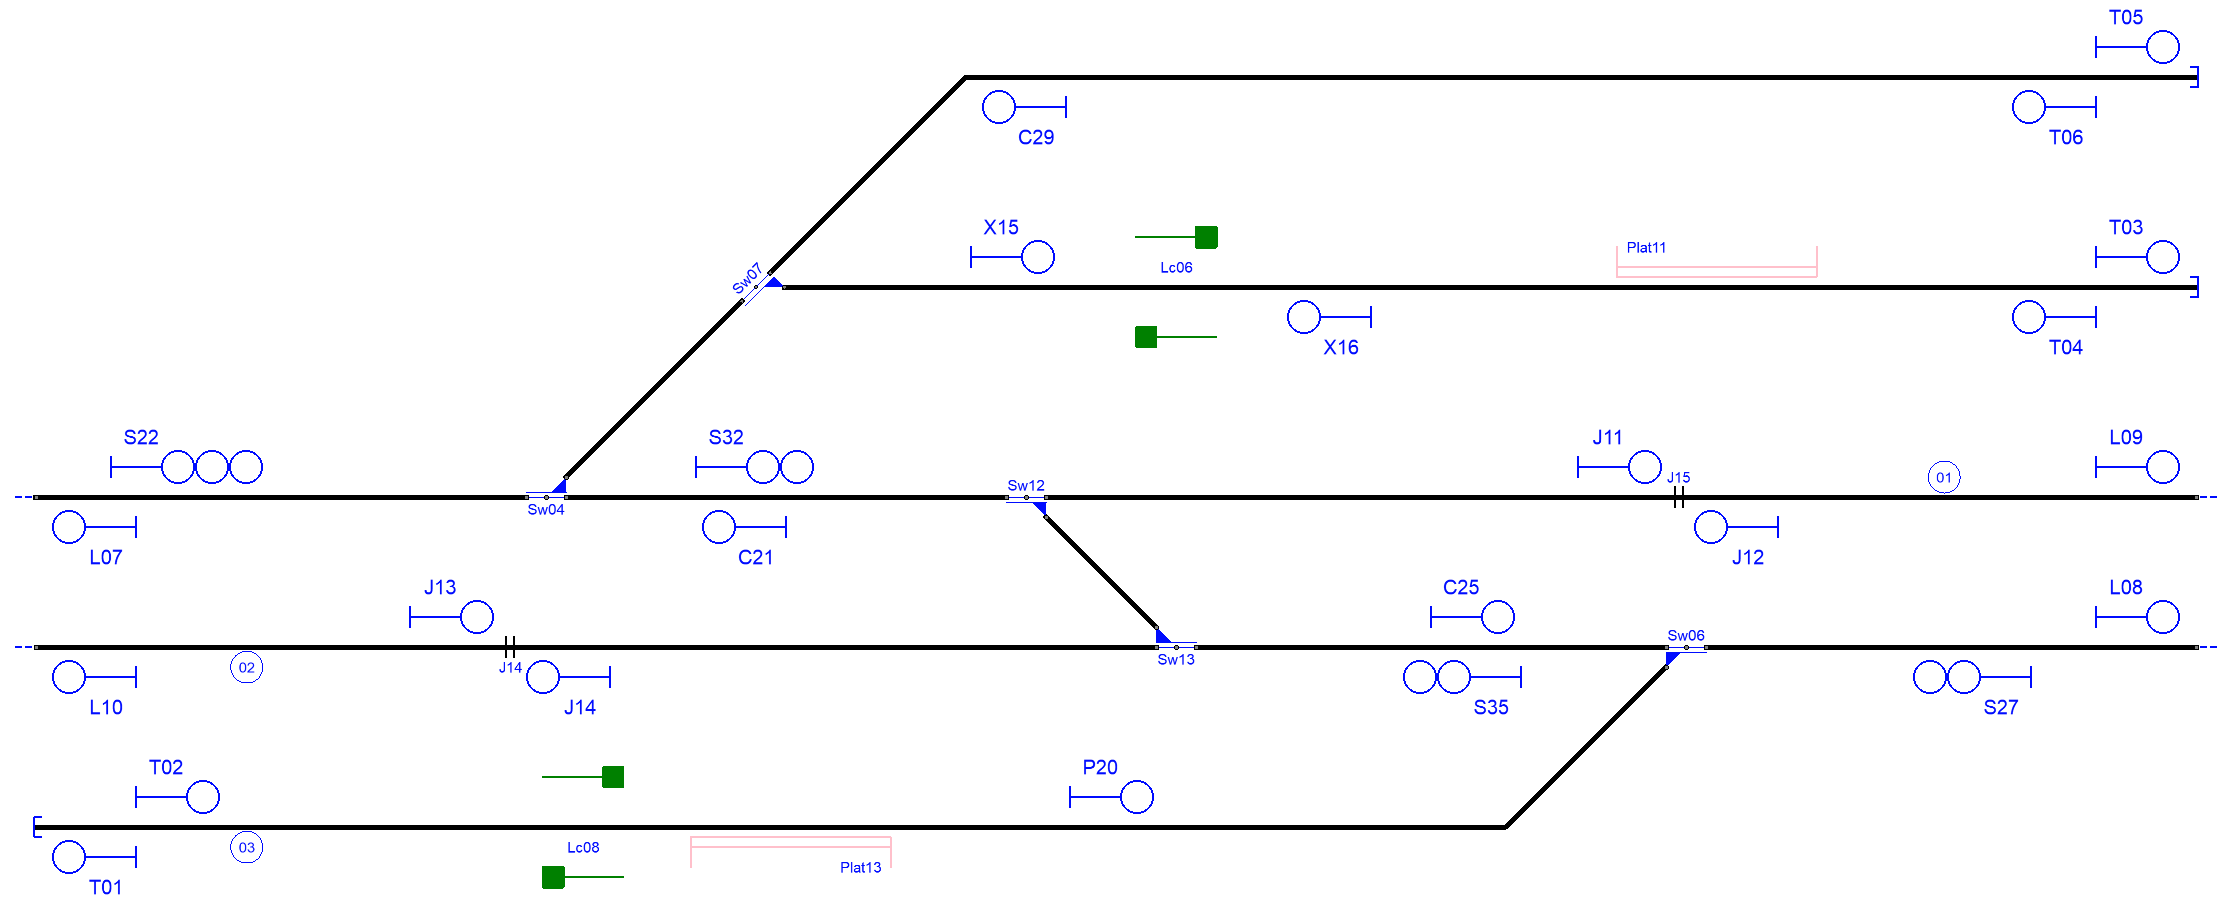
\includegraphics[width=1\textwidth]{resultados-obtenidos/ejemplo1/images/1_RNA.png}
        \centering\caption{Señalamiento generado y simplificado por el RNA.}
        %\label{fig:LC_P2}
    \end{figure}
    
    \subsection{Señalamiento original}

    El señalamiento diseñado en forma manual por el autor de esta tesis para la topología de la Figura \ref{fig:EJ1_1} se ilustra en la Figura \ref{fig:EJ1_2}. Se observa que incluye señales de parada próximas a los finales de vías absolutos (S18, S19, S20), señales de partida en las plataformas (S04, S06, S08, S09), señales de protección antes de cada paso a nivel (S04, S05), señales de maniobras antes de converger en una vía principal (S03, S08) y señales múltiples para cambios de vías divergentes (S01, S17, S10, S07), entre varias otras señales. Estas señales permiten definir hasta un máximo de 14 rutas, todas ellas detalladas en la Tabla \ref{Tab:tabla_original_1}
    
    \begin{figure}[H]
    	\centering
    	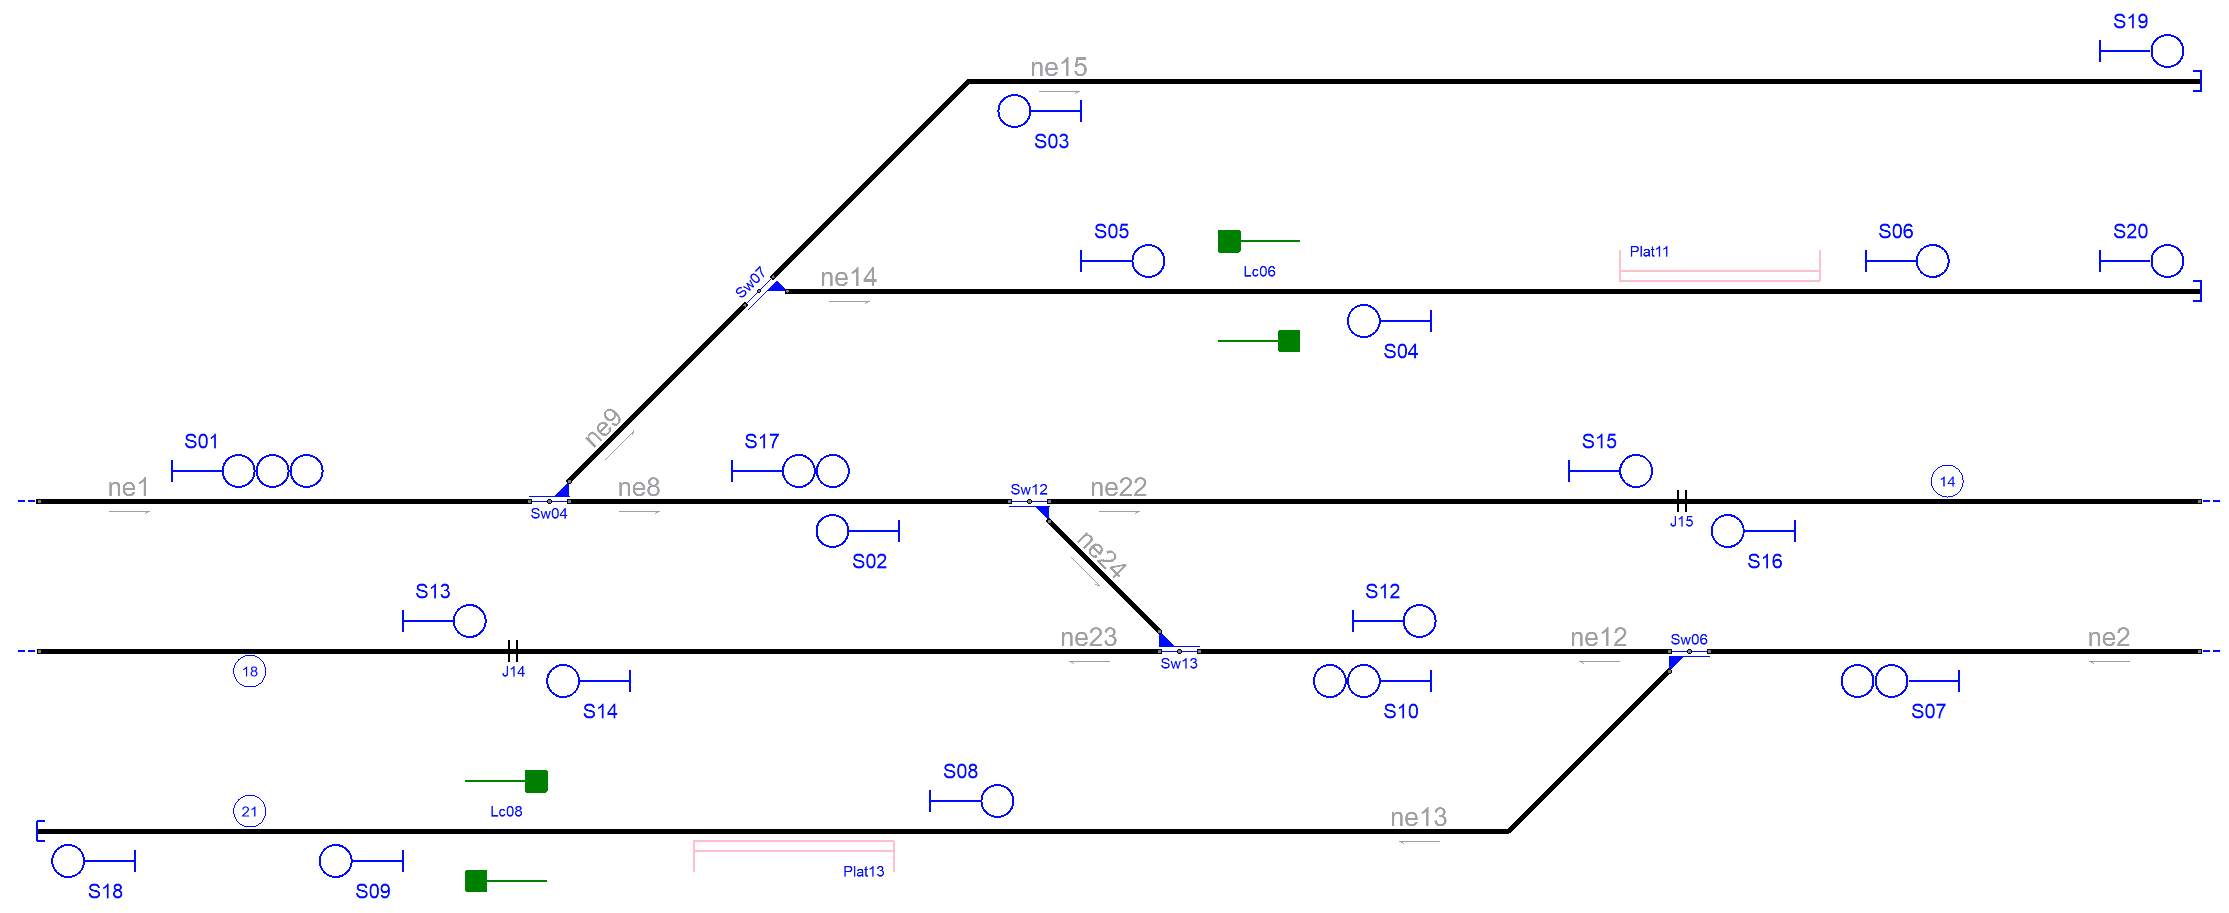
\includegraphics[width=1\textwidth]{resultados-obtenidos/ejemplo1/images/1_original.png}
    	\centering\caption{Señalamiento original del ejemplo 1.}
    	\label{fig:EJ1_2}
    \end{figure}
    
    En una primera inspección, se puede comprobar que todos los elementos ferroviarios son alcanzados por al menos una de las rutas, en al menos una dirección. Además, todos los cambios de vías son utilizados, de forma simple o compuesta. 
    
    \begin{table}[H]
        {
        \caption{Tabla de enclavamiento original del ejemplo 1.}
        \label{Tab:tabla_original_1}
        \centering
        \resizebox{1\textwidth}{!}{
            \begin{tabular}{ c c c c c c c }
                \hline	
                    Ruta & Inicio & Final & Cambio & Plataforma & Cruce & netElement \\	
                \hline
                    R$_{01}$  & S$_{05}$ & S$_{06}$ & - & Plat$_{11}$ & Lc$_{06}$ & ne$_{14}$\\
                    R$_{02}$  & S$_{06}$ & S$_{20}$ & - & - & - & ne$_{14}$\\
                    R$_{03}$  & S$_{09}$ & S$_{18}$ & - & - & - & ne$_{13}$\\
                    R$_{04}$  & S$_{13}$ & S$_{12}$ & Sw$_{13}^{N}$ & - & - & ne$_{23}$-ne$_{12}$\\
                    R$_{05}$  & S$_{16}$ & S$_{02}$ & Sw$_{12}^{N}$ & - & - & ne$_{22}$-ne$_{08}$\\
                    R$_{06}$  & S$_{07}$ & S$_{10}$ & Sw$_{06}^{N}$ & - & - & ne$_{02}$-ne$_{12}$\\
                    R$_{07}$  & S$_{07}$ & S$_{09}$ & Sw$_{06}^{R}$ & Plat$_{13}$ & Lc$_{08}$ & ne$_{02}$-ne$_{13}$\\
                    R$_{08}$  & S$_{10}$ & S$_{14}$ & Sw$_{13}^{N}$ & - & - & ne$_{12}$-ne$_{23}$\\
                    R$_{09}$  & S$_{10}$ & S$_{02}$ & Sw$_{12}^{R}$+Sw$_{13}^{R}$ & - & - & ne$_{12}$-ne$_{24}$-ne$_{08}$\\
                    R$_{10}$  & S$_{01}$ & S$_{17}$ & Sw$_{04}^{N}$ & - & - & ne$_{01}$-ne$_{08}$\\
                    R$_{11}$  & S$_{01}$ & S$_{19}$ & Sw$_{04}^{R}$+Sw$_{07}^{N}$ & - & - & ne$_{01}$-ne$_{15}$\\
                    R$_{12}$  & S$_{01}$ & S$_{05}$ & Sw$_{04}^{R}$+Sw$_{07}^{R}$ & - & - & ne$_{01}$-ne$_{14}$\\
                    R$_{13}$  & S$_{17}$ & S$_{15}$ & Sw$_{12}^{N}$ & - & - & ne$_{08}$-ne$_{22}$\\
                    R$_{14}$  & S$_{17}$ & S$_{12}$ & Sw$_{12}^{R}$+Sw$_{13}^{R}$ & - & - & ne$_{08}$-ne$_{24}$-ne$_{12}$\\    
                \hline
            \end{tabular}
        }
     }
    \end{table}
    
    Algunas rutas abarcan mas de un \textit{netElement}, como por ejemplo la ruta R14 que comienza en la señal S17 y finaliza en la señal S12, atraviesa los \textit{netElements} ne8, ne24 y ne12, y utiliza los cambios de vías Sw12 y Sw13, ambos en posición reversa.

    \subsection{Señalamiento generado por el RNA}

    \lipsum[1]
    
    \begin{table}[!h]
        {
        \caption{Tabla de enclavamiento del ejemplo 1 generada por el RNA.}
        \label{Tab:tabla_generated_1}
        \centering
        \resizebox{1\textwidth}{!}{
            \begin{tabular}{ c c c c c c c }
                \hline	
                    Ruta & Inicio & Final & Cambio & Plataforma & Cruce & netElement \\	
                \hline
                    R$_{01}$  & T$_{02}$ & P$_{20}$ & - & Plat$_{13}$ & Lc$_{08}$ & ne$_{13}$\\
                    R$_{02}$  & T$_{04}$ & X$_{16}$ & - & Plat$_{11}$ & - & ne$_{14}$\\
                    R$_{03}$  & T$_{06}$ & C$_{29}$ & - & - & - & ne$_{15}$\\
                    R$_{04}$  & J$_{11}$ & L$_{09}$ & - & - & - & ne$_{22}$\\
                    R$_{05}$  & J$_{12}$ & C$_{21}$ & Sw$_{12}^{N}$ & - & - & ne$_{22}$-ne$_{08}$\\
                    R$_{06}$  & J$_{13}$ & C$_{25}$ & Sw$_{13}^{N}$ & - & Lc$_{08}$ & ne$_{23}$-ne$_{12}$\\
                    R$_{07}$  & X$_{15}$ & T$_{03}$ & - & Plat$_{11}$ & Lc$_{06}$ & ne$_{14}$\\
                    R$_{08}$  & X$_{16}$ & L$_{07}$ & Sw$_{04}^{R}$+Sw$_{07}^{R}$ & - & - & ne$_{14}$-ne$_{01}$\\
                    R$_{09}$  & P$_{20}$ & L$_{08}$ & Sw$_{06}^{R}$ & - & - & ne$_{13}$-ne$_{02}$\\
                    R$_{10}$  & C$_{21}$ & L$_{07}$ & Sw$_{04}^{N}$ & - & - & ne$_{08}$-ne$_{01}$\\
                    R$_{11}$  & S$_{22}$ & S$_{32}$ & Sw$_{04}^{N}$ & - & - & ne$_{01}$-ne$_{08}$\\
                    R$_{12}$  & S$_{22}$ & X$_{15}$ & Sw$_{04}^{R}$+Sw$_{07}^{R}$ & - & - & ne$_{01}$-ne$_{14}$\\
                    R$_{13}$  & S$_{22}$ & T$_{05}$ & Sw$_{04}^{R}$+Sw$_{07}^{N}$ & - & - & ne$_{01}$-ne$_{15}$\\
                    R$_{14}$  & C$_{25}$ & L$_{08}$ & Sw$_{06}^{N}$ & - & - & ne$_{12}$-ne$_{02}$\\
                    R$_{15}$  & S$_{27}$ & S$_{35}$ & Sw$_{06}^{N}$ & - & - & ne$_{02}$-ne$_{12}$\\
                    R$_{16}$  & S$_{27}$ & T$_{01}$ & Sw$_{06}^{R}$ & Plat$_{13}$ & Lc$_{08}$ & ne$_{02}$-ne$_{13}$\\
                    R$_{17}$  & C$_{29}$ & L$_{07}$ & Sw$_{04}^{R}$+Sw$_{07}^{N}$ & - & - & ne$_{15}$-ne$_{01}$\\
                    R$_{18}$  & S$_{32}$ & J$_{11}$ & Sw$_{12}^{N}$ & - & - & ne$_{08}$-ne$_{22}$\\
                    R$_{19}$  & S$_{32}$ & C$_{25}$ & Sw$_{12}^{R}$+Sw$_{13}^{R}$ & - & - & ne$_{08}$-ne$_{12}$\\
                    R$_{20}$  & S$_{35}$ & J$_{14}$ & Sw$_{13}^{N}$ & - & - & ne$_{12}$-ne$_{23}$\\
                    R$_{21}$  & S$_{35}$ & C$_{21}$ & Sw$_{12}^{R}$+Sw$_{13}^{R}$ & - & - & ne$_{12}$-ne$_{08}$\\
                \hline
            \end{tabular}
        }
     }
    \end{table}
    \subsection{Sistema generado por el ACG}
	\label{sec:EJEMPLO1_ACG}
	
	En base a la red de grafos, ilustrada en la Figura \ref{fig:EJ1_8}, el ACG determinó la cantidad de elementos ferroviarios de cada tipo, tal como puede visualizarse en el Código \ref{lst:EJ1_8}.
	
	\begin{lstlisting}[language = {}, caption = Cantidad de elementos a implementar por el ACG, label = {lst:EJ1_8}]
	n_netElements:11
	n_switch:5
	n_doubleSwitch:0
	n_borders:4
	n_buffers:3
	n_levelCrossings:2
	n_platforms:2
	n_scissorCrossings:0
	n_signals:23
	N : 62
	\end{lstlisting}
	
	El ACG genera, en el caso de este ejemplo, 80 archivos en formato VHDL, tal como se puede visualizar en la Figura \ref{fig:EJ1_ACG_1}. Podemos destacar de la Figura \ref{fig:EJ1_ACG_1} al archivo \textit{Arty\_Z7-10.XDC}, que define los pines de entrada y salida de la plataforma Arty Z7 10 y Arty Z7 20. Este archivo es provisto por Xilinx para esta familia de plataformas. En caso de utilizar otra plataforma, se deberá incluir el archivo XDC correspondiente. En ambos casos, cada desarrollador debe asignar manualmente los pines a cada puerto del sistema generado por el ACG.
	
	\begin{figure}[H]
		\centering
		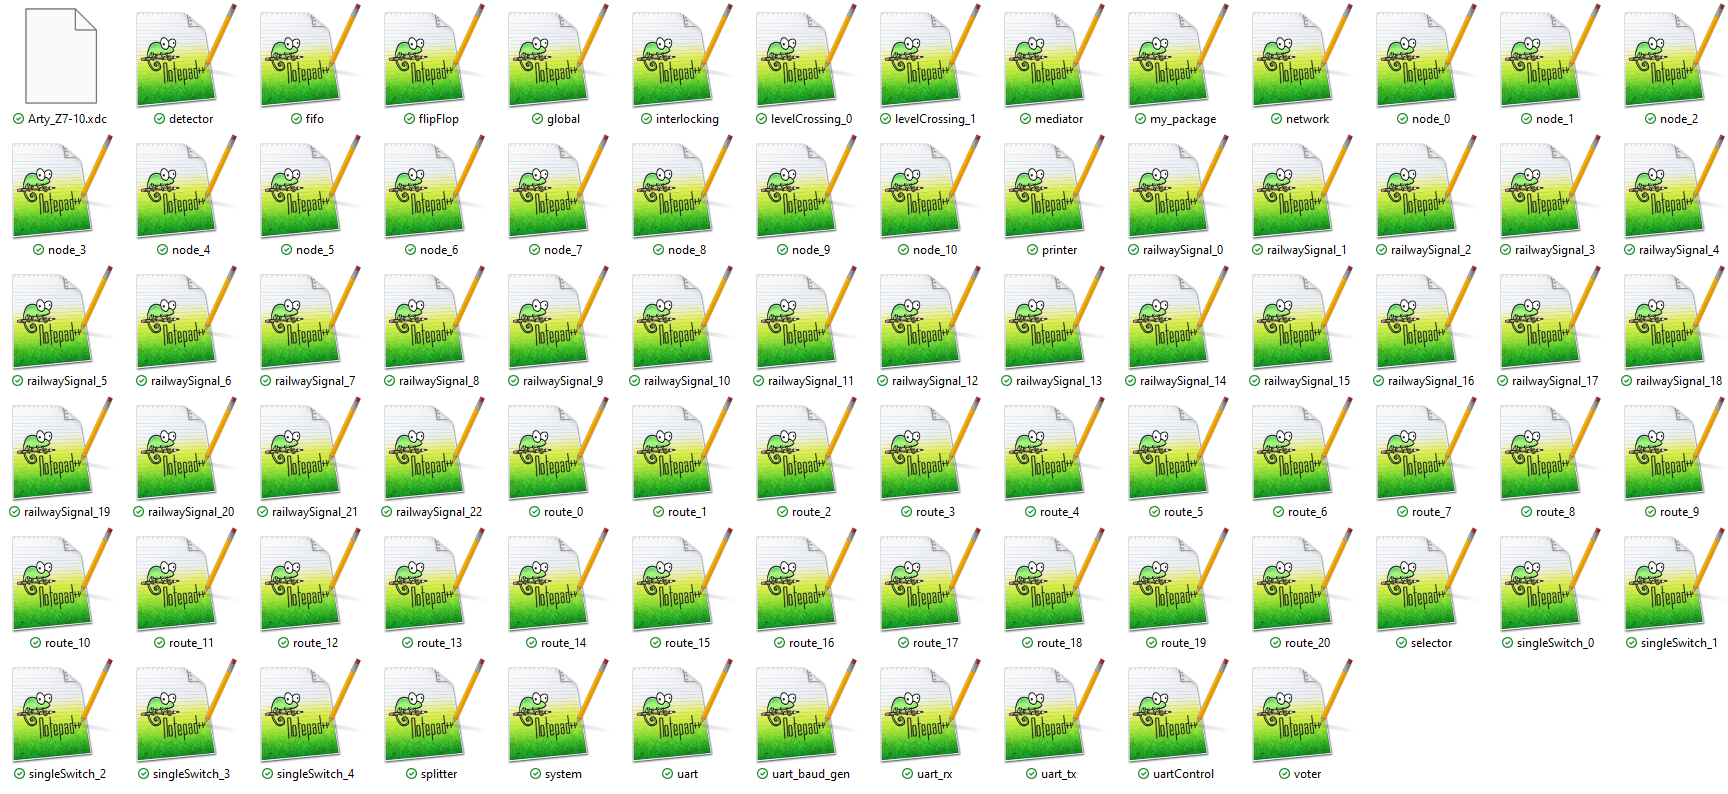
\includegraphics[origin = c, width=1\textwidth]{resultados-obtenidos/ejemplo1/images/ACG_files}
		\centering\caption{Archivos generador por el ACG para el ejemplo 1.}
		\label{fig:EJ1_ACG_1}
	\end{figure}
	
	Además, podemos mencionar los archivos \textit{my\_package.VHDL} y \textit{flipFlop.VHDL}, ambos generados por el ACG. El primero es una librería que define todos los tipos de datos utilizados por el sistema, y el segundo es un flip-flop tipo D utilizado para generar la secuencia de shift registers necesarios para adaptar el clock de entrada a los diferentes dominios de clock necesarios para el timeout de cada elemento ferroviario.
	
	Los archivos restantes son archivos que definen los módulos de alto nivel explicados en la Sección \ref{sec:interlockingArch} o la representación en VHDL de cada elemento ferroviario explicado entre la Sección \ref{sec:ACG_lc} y la Sección \ref{sec:ACG_rts}. Por ejemplo, en base lo descrito en el Código \ref{lst:EJ1_8}, hay 23 señales ferroviarias y podemos visualizar en la Figura \ref{fig:EJ1_ACG_1} 23 archivos referidos a las señales ferroviarias: desde \textit{railwaySignal\_0} hasta \textit{railwaySignal\_22}.
	
	Cada ejemplo cuenta con su propia carpeta de principio a fin. Es decir, el archivo railML original, los archivos generados por el RNA y el código generado por el ACG se encuentran en carpetas individuales para cada ejemplo. Esto es una ventaja a la hora de mantener un orden pero una gran desventaja a la hora de sintetizar los proyectos en Vivado. Cada conjunto de archivos debería ser importado de manera individual, previa desvinculación de los archivos del proyecto anterior. Para solucionar este inconveniente se desarrolló el Código \ref{lst:EJ1_script}, que automatiza la importación y desvinculación de los archivos de cada ejemplo.
	
	
	\begin{lstlisting}[language = {bash}, caption = script.tcl, label = {lst:EJ1_script}]
set chosen 1

# Get a list of all design source files
set design_sources [get_files -of_objects [get_filesets sources_1]]

remove_files $design_sources

set base_folder_path "ROOT/GICSAFePhD/App/Layouts/Example_"
set folder_path "${base_folder_path}${chosen}/VHDL"

puts $folder_path

set files [glob -directory $folder_path *.vhd]

add_files -norecurse -scan_for_includes  $files

update_compile_order -fileset sources_1
update_compile_order -fileset sources_1

synth_design -rtl -rtl_skip_mlo -name rtl_1
	\end{lstlisting}
	
	El parámetro \textit{chosen} indica el número de ejemplo seleccionado, mientras que \textit{base\_folder\_path} es la ruta absoluta de los ejemplos, cuyas carpetas deben ser nombradas como \textit{Example\_}+\textit{chosen} para poder ser encontradas. El Código \ref{lst:EJ1_script} puede ser importado en Vivado desde \textit{Tools $>$ Custom Commands $>$ Customize Commands} como un archivo TCL (del inglés, Tool Command Language), que es el formato que define los comandos nativos de Vivado. Pueden importarse tantos archivos TCL como se deseen, uno por cada ejemplo a sintetizar. De esta manera, cada script aparecerá en la barra de acceso rápido de Vivado de forma independiente y se automatiza el proceso de sincronización de archivos.
	
	Una vez ejecutado el script, Vivado ordenará los archivos de forma jerárquica, como puede verse en la parte izquierda de la Figura \ref{fig:EJ1_ACG_Vivado} donde el módulo \textit{global} incluye todos los módulos que fueron detallados en la Sección \ref{sec:interlockingArch}. Podemos destacar al módulo \textit{network} que es instanciado 3 veces junto con el módulo \textit{voter}, al ser una redundancia 2oo3, tal fue explicado en la Sección \ref{sec:VHDL2oo3}. Cada una de las instancias del módulo \textit{network} contienen sus propias 62 instancias de los mismos módulos de cada elemento ferroviario ya que N, cantidad de elementos ferroviarios, es 62 en el Código \ref{lst:EJ1_8}.	
	
	\begin{figure}[H]
		\centering
		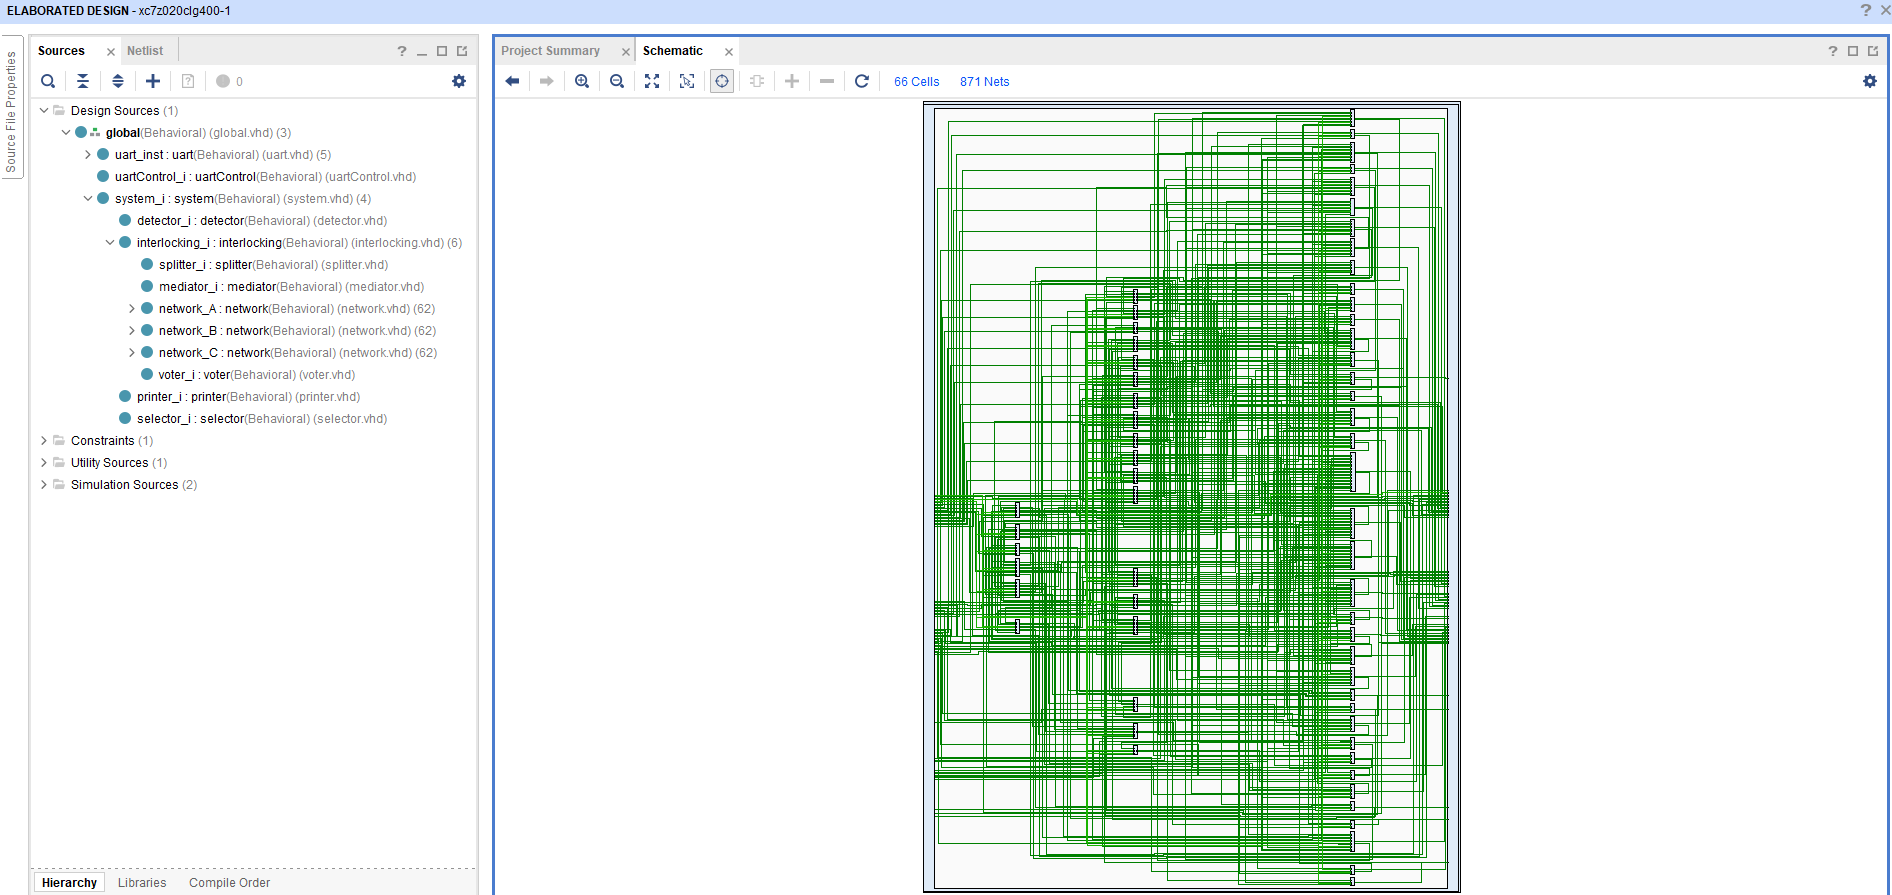
\includegraphics[origin = c, width=1\textwidth]{resultados-obtenidos/ejemplo1/images/ACG_vivado}
		\centering\caption{Interfaz del entorno de desarrollo Vivado para el ejemplo 1.}
		\label{fig:EJ1_ACG_Vivado}
	\end{figure}
	
	La parte derecha de la Figura \ref{fig:EJ1_ACG_Vivado} ilustra la representación en diagrama de bloques de uno de los módulos \textit{network} (los tres módulos tienen los mismos bloques). Puede apreciarse en esta ventana que existen 66 módulos interconectados de forma compleja utilizando 871 señales. Pero esto es solamente una porción del sistema generado por el ACG, de inspeccionar cada uno de los bloques es posible determinar que el ejemplo 1 utiliza 9517 sub módulos conectados automáticamente mediante 21899 señales, lo cual se aleja bastante de un desarrollo que pueda realizarse manualmente de forma trivial.
	
	Una vez que Vivado ha generado el diagrama de bloques ya tenemos la certeza de que el código VHDL ha pasado la prueba de sintaxis del entorno de desarrollo. A continuación, se deberá sintetizar e implementar el sistema para generar el bitstream que será utilizado para programar la FPGA. Durante el proceso de síntesis, Vivado busca la mejor forma de representar el código VHDL con compuertas lógicas, por lo que un código de mejor calidad brindará una representación en hardware lo mas fiel posible a lo buscado. Durante el proceso de implementación, en cambio, Vivado calcula si la representación con compuertas lógicas es posible de realizarse con la plataforma disponible. En este proceso influye no solamente la cantidad de compuertas disponibles sino también el tipo de compuertas. Si la plataforma no cuenta con la cantidad suficiente de compuertas A, entonces Vivado buscará la forma de reemplazar esa compuerta por otras compuertas B, C o D, que sean su equivalente lógico. Este proceso de reemplazo y/o simplificación puede llevar a que ambos procesos presenten discrepancias en la cantidad de elementos utilizados. 
	
	Los resultados de ambos procesos son detallados en la Tabla \ref{Tab:tabla_ACG_1}. Los porcentajes de uso son calculados por Vivado automáticamente, teniendo en cuenta que la plataforma Arty Z7 20 posee 53200 Look-Up-Tables (LUTs), 106400 Flip-Flops (FFs), 125 Pines de entrada y salida (IOs) y 32 Buffers (BUFGs), tal cómo se explicó en la Sección \ref{sec:AGG}. En este ejemplo, la cantidad de recursos utilizados es baja y el tiempo de síntesis e implementación es de 47 y 44 segundos, respectivamente.
	
	\begin{table}[H]
		{
			\caption{Síntesis e implementación del ejemplo 1 generado por el ACG.}
			\label{Tab:tabla_ACG_1}
			\centering
			%\small
			%\centering
			\begin{center}
				\resizebox{0.7\textwidth}{!}{
					\begin{tabular}{ c c c c }
						\hline	
						Recursos & Síntesis & Implementación & Uso \\	
						\hline
						LUT & 3457 & 3416 & 6.42/6.50\%\\
						FF & 3810 & 3813 & 3.58\%\\
						IO & 15 & 15 & 12.00\%\\
						BUFG & 3 & 3 & 9.38\%\\
						\hline
					\end{tabular}
				}
			\end{center}
		}    
	\end{table}
	
	
	
    \subsection{Validación del sistema de enclavamientos}

    Las 14 rutas del señalamiento original (Tabla \ref{Tab:tabla_original_1}) tienen 14 rutas equivalentes en el señalamiento generado por el RNA (Tabla \ref{Tab:tabla_generated_1}), tal como se puede visualizar en la Tabla \ref{Tab:tabla_validation_1}, generada automáticamente por el RNA.

    \begin{table}[H]
        {
        \caption{Equivalencias entre las rutas originales y las generadas por el RNA.}
        \label{Tab:tabla_validation_1}
        \centering
        %\small
            %\centering
            \begin{center}
            \resizebox{0.7\textwidth}{!}{
            \begin{tabular}{ c c c c }
                \hline	
                    Original & Señales & RNA & Señales \\	
                \hline
                    R$_{01}$ & S$_{05}$-S$_{06}$ & R$_{07}$ & X$_{15}$-T$_{03}$ \\
                    R$_{02}$ & S$_{06}$-S$_{20}$ & R$_{07}$ & X$_{15}$-T$_{03}$ \\
                    R$_{03}$ & S$_{09}$-S$_{18}$ & R$_{16}$ & S$_{27}$-T$_{01}$ \\
                    R$_{04}$ & S$_{13}$-S$_{12}$ & R$_{06}$ & J$_{13}$-C$_{25}$ \\
                    R$_{05}$ & S$_{16}$-S$_{02}$ & R$_{05}$ & J$_{12}$-C$_{21}$ \\
                    R$_{06}$ & S$_{07}$-S$_{10}$ & R$_{15}$ & S$_{27}$-S$_{35}$ \\
                    R$_{07}$ & S$_{07}$-S$_{09}$ & R$_{16}$ & S$_{27}$-T$_{01}$ \\
                    R$_{08}$ & S$_{10}$-S$_{14}$ & R$_{20}$ & S$_{35}$-J$_{14}$ \\
                    R$_{09}$ & S$_{10}$-S$_{02}$ & R$_{21}$ & S$_{35}$-C$_{21}$ \\
                    R$_{10}$ & S$_{01}$-S$_{17}$ & R$_{11}$ & S$_{22}$-S$_{32}$ \\
                    R$_{11}$ & S$_{01}$-S$_{19}$ & R$_{13}$ & S$_{22}$-X$_{15}$ \\
                    R$_{12}$ & S$_{01}$-S$_{05}$ & R$_{12}$ & S$_{22}$-T$_{05}$ \\
                    R$_{13}$ & S$_{17}$-S$_{15}$ & R$_{18}$ & S$_{32}$-J$_{11}$ \\
                    R$_{14}$ & S$_{17}$-S$_{12}$ & R$_{19}$ & S$_{32}$-C$_{25}$ \\   
                \hline
            \end{tabular}
            }
            \end{center}
        }    
    \end{table}
    
    Las rutas R1, R2, R3, R4, R7, R8, R9, R10, R13, R14 y R16 (Tabla \ref{Tab:tabla_generated_1}) generadas por el RNA que no tienen equivalencias en el señalamiento original (Tabla \ref{Tab:tabla_original_1}) se deben a que el RNA creó señales extras. Las señales T01, T02, T03, T04, T05 y T06 fueron creadas por el RNA para proteger los finales de vía absolutos, mientras que las señales L07, L08, L09 y L10 fueron creadas para proteger los finales de vías relativos. Estas nuevas señales constituyen nuevas rutas que permiten a las formaciones detenerse previo al final (relativo o absoluto) de la red ferroviaria, lo cual incrementa la seguridad y añade nuevas rutas en sentido contrario, mejorando la logística. Estos elementos ferroviarios no se encontraban protegidos en el señalamiento original.
    
    El señalamiento original carecía de señales protegiendo los finales de vía absolutos y relativos. No obstante, esto no se debe a un error en el diseño original, sino a que el diseño de señalamientos en la vida real se encuentra restringido por las necesidades particulares de cada locación, operador o leyes locales. Algunos operadores priorizarán tener rutas largas, dejando largas distancias sin señalamiento electrónico. Algunas normativas pueden indicar que la protección de ciertos elementos puede ser optativa. En el caso de los finales de vía pueden utilizarse señales lumínicas intermitentes que no son controladas por el señalamiento.
    
    En otros ejemplos el señalamiento original puede estar "incompleto", es decir, solo se consideraron las rutas en un sentido determinado, en base al uso que se le quería dar a ese señalamiento. El RNA, en cambio, siempre generará el señalamiento completo, que abarque la totalidad de la red ferroviaria ingresada, a menos que se seleccione la opción de señalamiento parcial, que respetará el sentido único de circulación que se defina en cada vía.    
    
    %TODO VALIDACION ALGORITMOS
    
    
    
    
    
	%\section{Ejemplo 2}

    \lipsum[1]
    
    \begin{figure}[h]
    	\centering
    	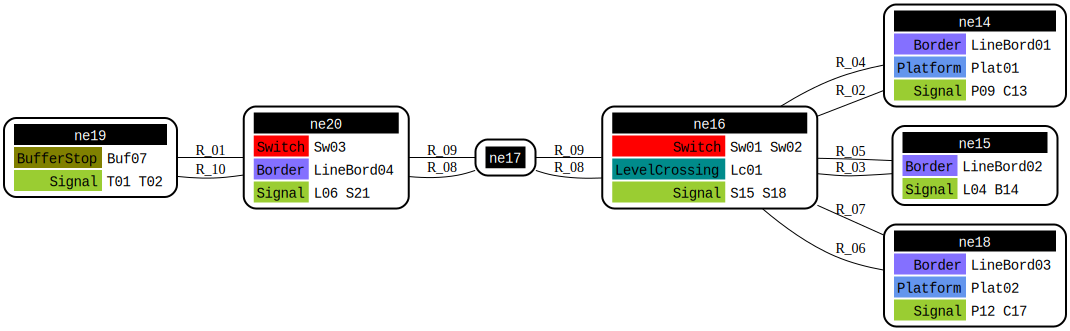
\includegraphics[width=1\textwidth]{Figuras/Graph_2}
    	\centering\caption{XXXX}
    	%\label{fig:LC_P2}
    \end{figure}
    
    \lipsum[1]

    \begin{figure}[h]
        \centering
        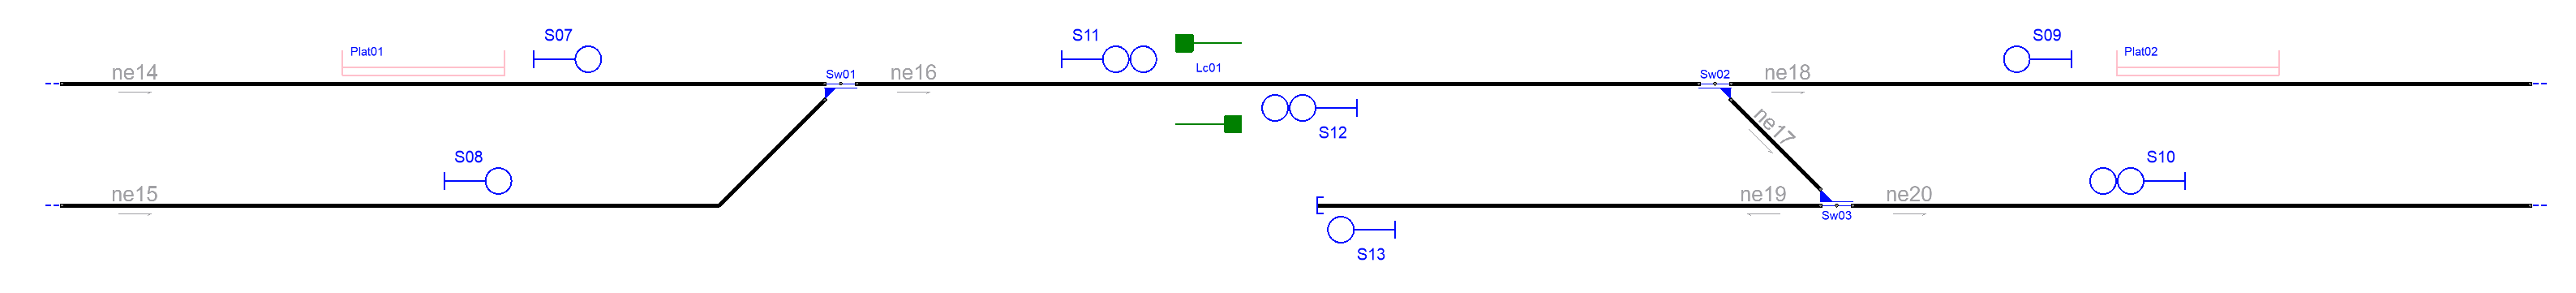
\includegraphics[width=1\textwidth]{resultados-obtenidos/ejemplo2/images/2_original.png}
        \centering\caption{Señalamiento original del ejemplo 2.}
        %\label{fig:LC_P2}
    \end{figure}

    \begin{figure}[h]
        \centering
        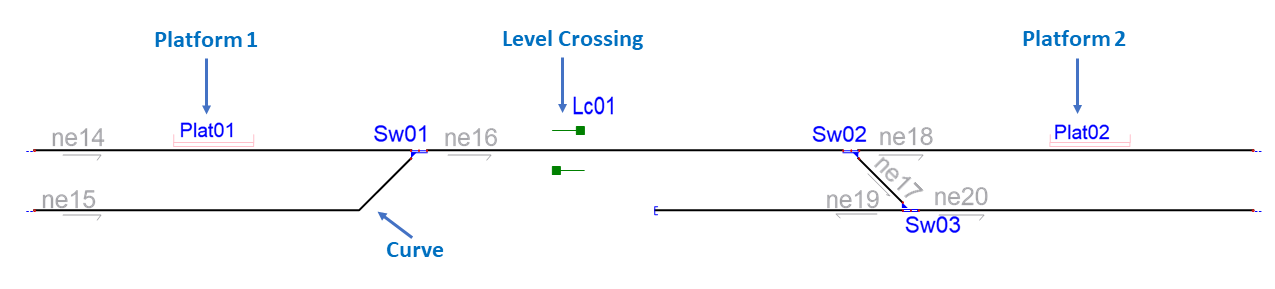
\includegraphics[width=1\textwidth]{resultados-obtenidos/ejemplo2/images/2_empty.png}
        \centering\caption{Topología ferroviaria del ejemplo 2 sin señalamiento.}
        %\label{fig:LC_P2}
    \end{figure}

    \begin{figure}[h]
        \centering
        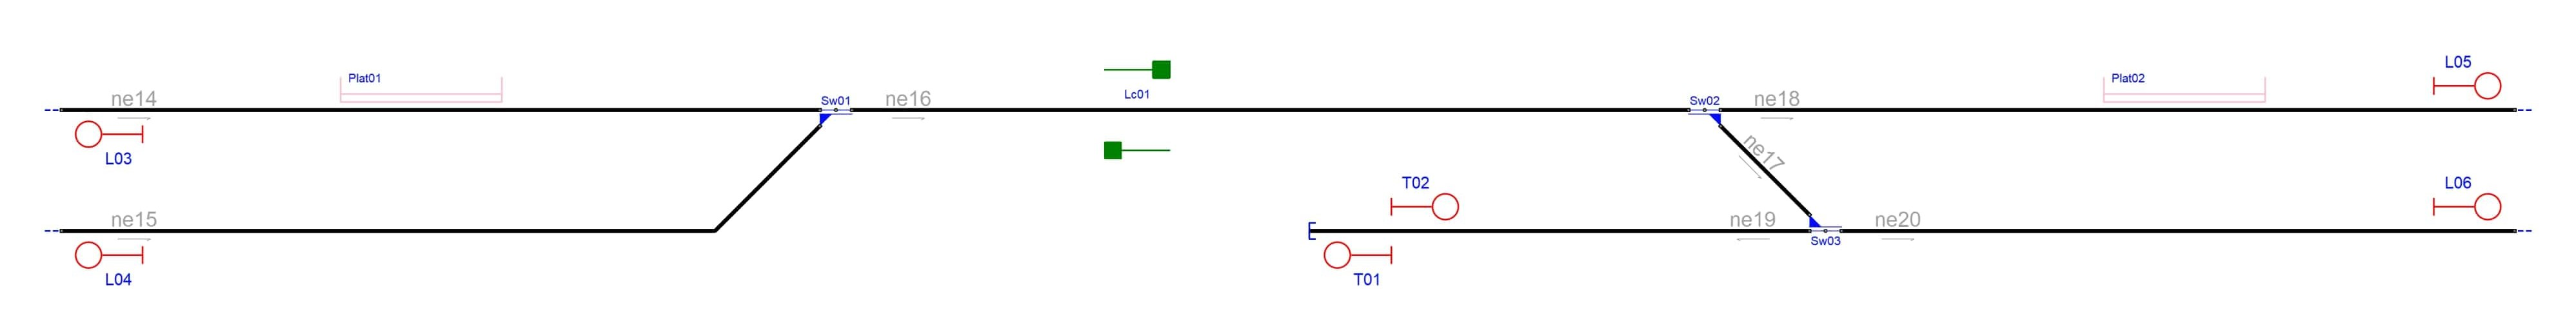
\includegraphics[width=1\textwidth]{resultados-obtenidos/ejemplo2/images/2_step1.png}
        \centering\caption{Señalamiento generado por el RNA para proteger el fín de vía.}
        %\label{fig:LC_P2}
    \end{figure}

    \begin{figure}[h]
        \centering
        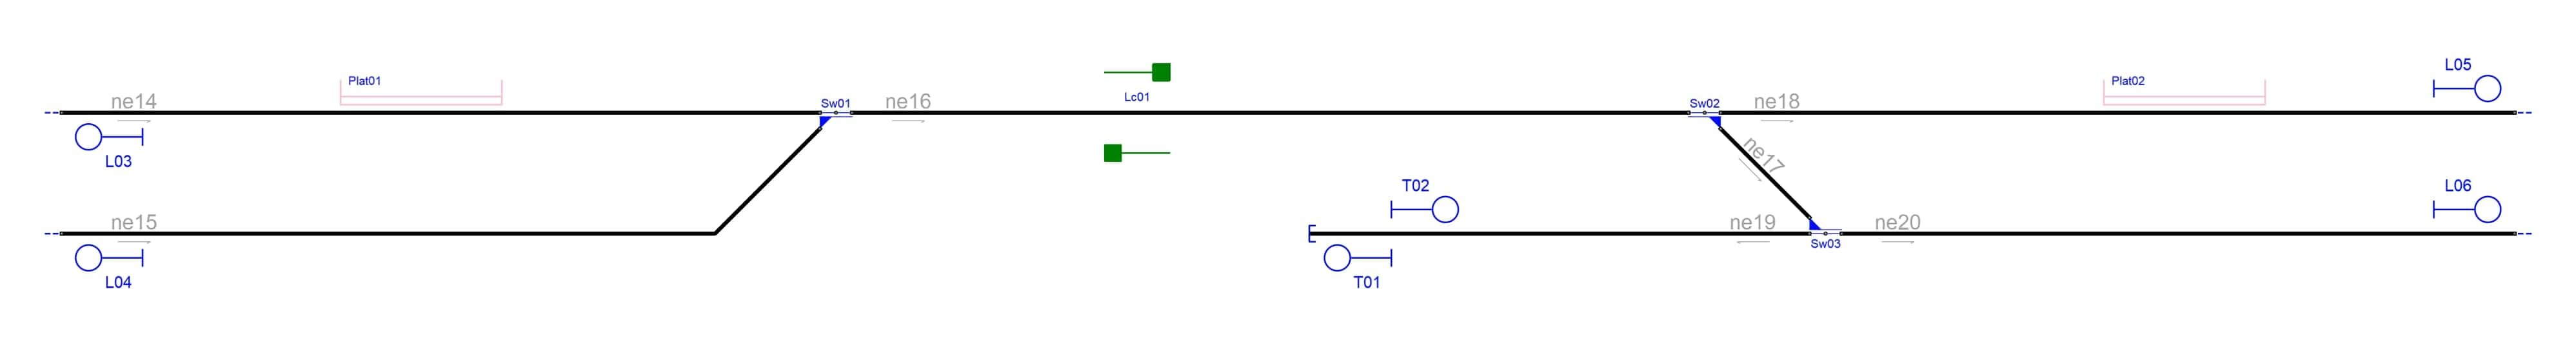
\includegraphics[width=1\textwidth]{resultados-obtenidos/ejemplo2/images/2_step2.png}
        \centering\caption{Señalamiento generado por el RNA para proteger las junturas.}
        %\label{fig:LC_P2}
    \end{figure}

    \begin{figure}[h]
        \centering
        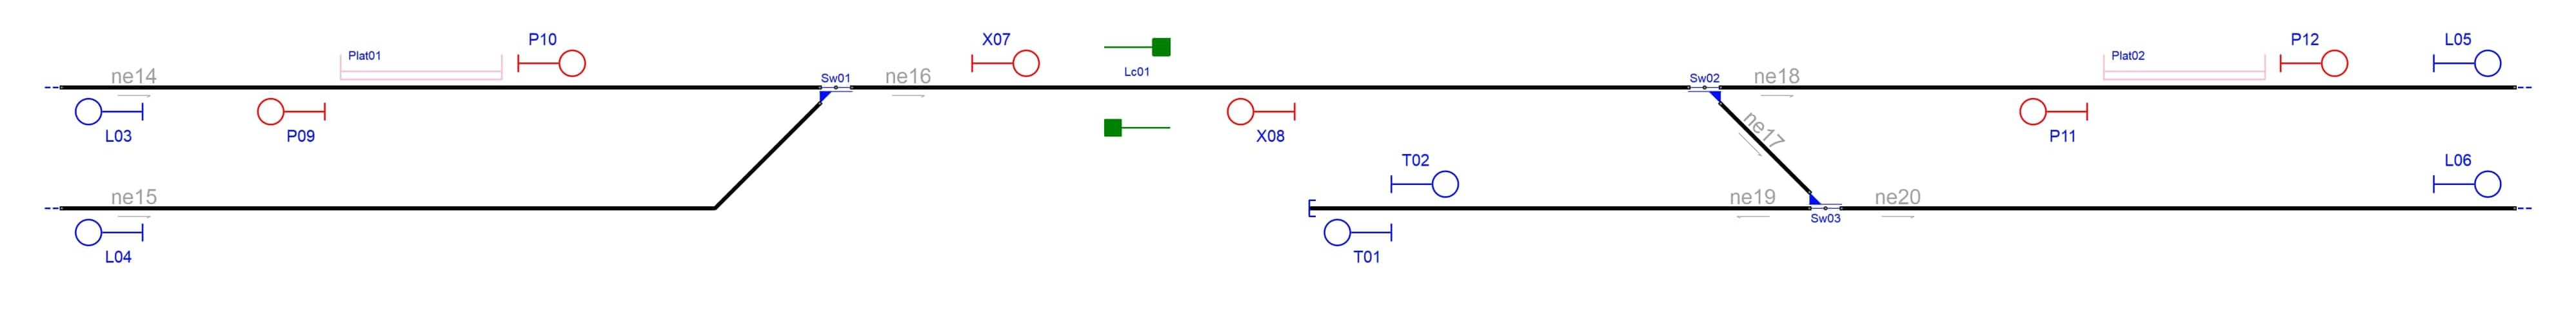
\includegraphics[width=1\textwidth]{resultados-obtenidos/ejemplo2/images/2_step3.png}
        \centering\caption{Señalamiento generado por el RNA para proteger plataformas y cruces de vía.}
        %\label{fig:LC_P2}
    \end{figure}

    \begin{figure}[h]
        \centering
        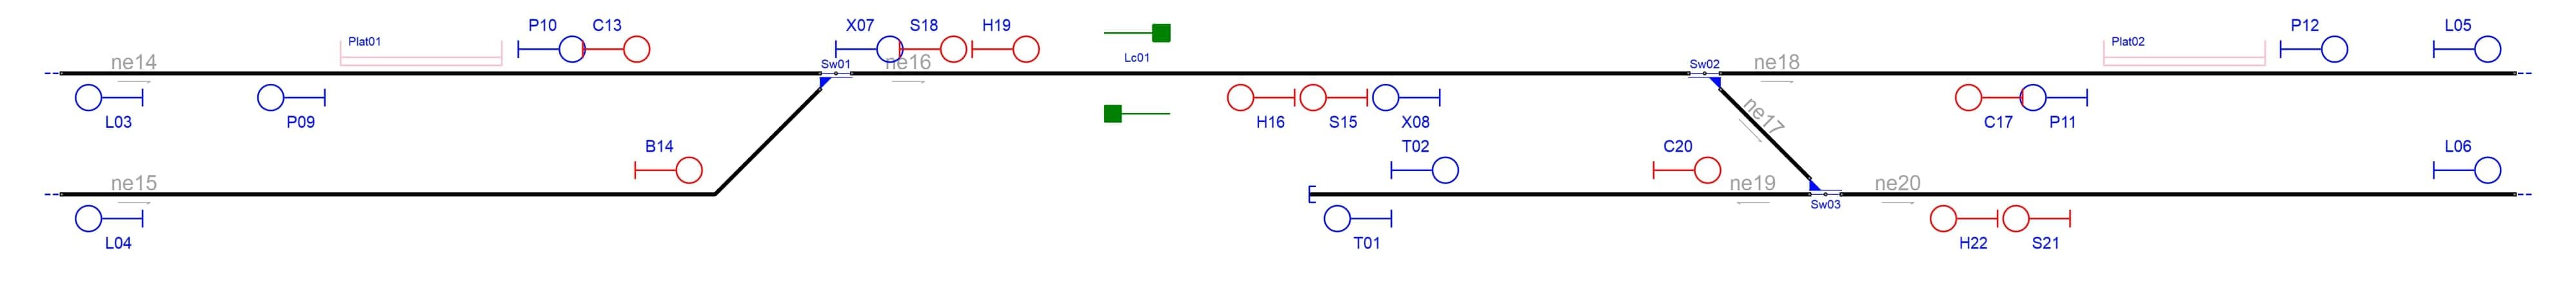
\includegraphics[width=1\textwidth]{resultados-obtenidos/ejemplo2/images/2_step4.png}
        \centering\caption{Señalamiento generado por el RNA para proteger las máquinas de cambios.}
        %\label{fig:LC_P2}
    \end{figure}

    \begin{figure}[h]
        \centering
        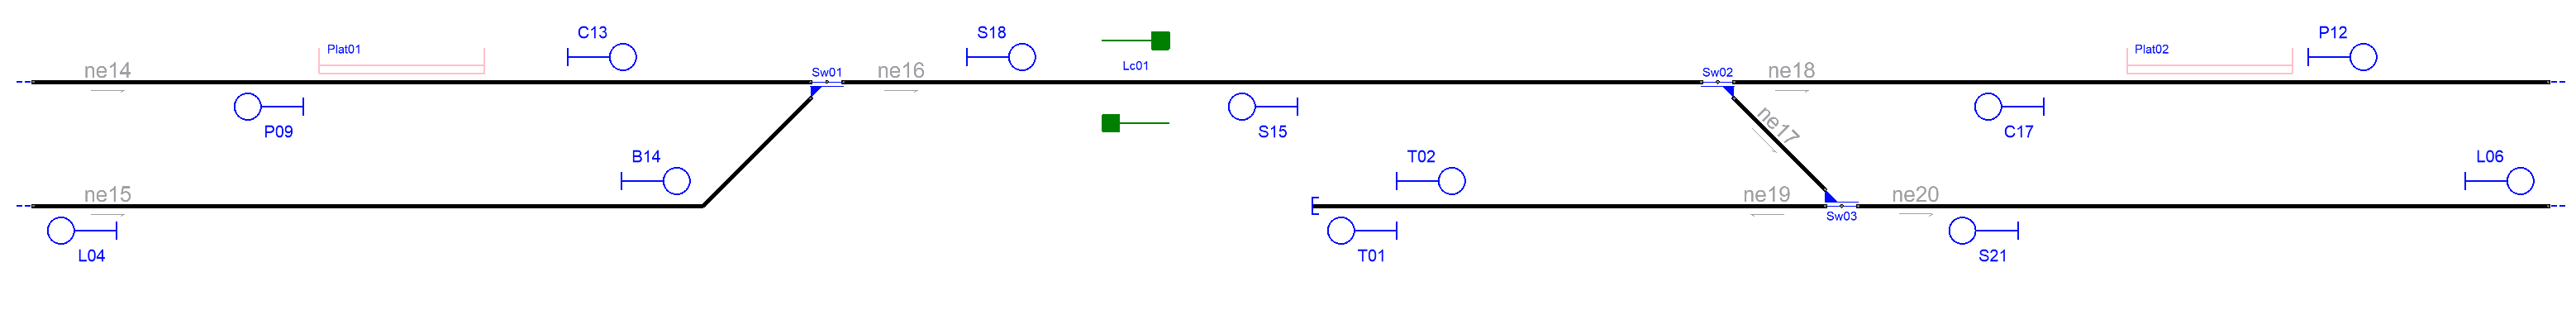
\includegraphics[width=1\textwidth]{resultados-obtenidos/ejemplo2/images/2_RNA.png}
        \centering\caption{Señalamiento generado y simplificado por el RNA.}
        %\label{fig:LC_P2}
    \end{figure}
    
    \subsection{Señalamiento original}

    \lipsum[1]
    
    \begin{table}[H]
        {
        \caption{Tabla de enclavamiento original del ejemplo 2.}
        \label{Tab:tabla_original_2}
        \centering
        \resizebox{1\textwidth}{!}{
            \begin{tabular}{ c c c c c c c }
                \hline	
                    Ruta & Inicio & Final & Cambio & Plataforma & Cruce & netElement \\	
                \hline
                    R$_{01}$  & S$_{07}$ & S$_{11}$ & Sw$_{01}^{N}$ & - & - & ne$_{14}$-ne$_{16}$\\
                    R$_{02}$  & S$_{08}$ & S$_{11}$ & Sw$_{01}^{R}$ & - & - & ne$_{15}$-ne$_{16}$\\
                    R$_{03}$  & S$_{09}$ & S$_{12}$ & Sw$_{02}^{N}$ & - & - & ne$_{18}$-ne$_{16}$\\
                    R$_{04}$  & S$_{10}$ & S$_{13}$ & Sw$_{03}^{N}$ & - & - & ne$_{20}$-ne$_{19}$\\
                    R$_{05}$  & S$_{10}$ & S$_{12}$ & Sw$_{03}^{R}$+Sw$_{02}^{R}$ & - & - & ne$_{20}$-ne$_{17}$-ne$_{16}$\\  
                \hline
            \end{tabular}
        }
     }
    \end{table}
    \section{Señalamiento generado por el RNA}

	El RNA también exporta la misma información mostrada en el Código \ref{lst:EJ2_8} en una hoja de cálculo, similar a la que se visualiza en la Tabla \ref{Tab:tabla_generated_2}.   
    
    \begin{table}[H]
        {
        \caption{Tabla de enclavamiento del ejemplo 2 generada por el RNA.}
        \label{Tab:tabla_generated_2}
        %\centering
        \begin{center}
        \resizebox{0.8\textwidth}{!}{
            \begin{tabular}{ c c c c c c c }
                \hline	
                    Ruta & Inicio & Final & Cambio & Plataforma & Cruce & netElement \\	
                \hline
                    R$_{01}$  & T$_{02}$ & L$_{06}$ & Sw$_{03}^{N}$ & - & - & ne$_{19}$-ne$_{20}$\\
                    R$_{02}$  & C$_{13}$ & S$_{18}$ & Sw$_{01}^{N}$ & - & - & ne$_{14}$-ne$_{16}$\\
                    R$_{03}$  & B$_{14}$ & S$_{18}$ & Sw$_{01}^{R}$ & - & - & ne$_{15}$-ne$_{16}$\\
                    R$_{04}$  & S$_{15}$ & P$_{09}$ & Sw$_{01}^{N}$ & Plat$_{01}$ & Lc$_{01}$ & ne$_{16}$-ne$_{14}$\\
                    R$_{05}$  & S$_{15}$ & L$_{04}$ & Sw$_{01}^{R}$ & Plat$_{01}$ & Lc$_{01}$ & ne$_{16}$-ne$_{15}$\\
                    R$_{06}$  & C$_{17}$ & S$_{15}$ & Sw$_{02}^{N}$ & - & - & ne$_{18}$-ne$_{16}$\\
                    R$_{07}$  & S$_{18}$ & P$_{12}$ & Sw$_{02}^{N}$ & Plat$_{02}$ & Lc$_{01}$ & ne$_{16}$-ne$_{18}$\\
                    R$_{08}$  & S$_{18}$ & L$_{06}$ & Sw$_{02}^{R}$+Sw$_{03}^{R}$ & - & Lc$_{01}$ & ne$_{16}$-ne$_{20}$\\
                    R$_{09}$  & S$_{21}$ & S$_{15}$ & Sw$_{02}^{R}$+Sw$_{03}^{R}$ & - & - & ne$_{20}$-ne$_{16}$\\
                    R$_{10}$  & S$_{21}$ & T$_{01}$ & Sw$_{03}^{N}$ & - & - & ne$_{20}$-ne$_{19}$\\
                \hline
            \end{tabular}
        }
        \end{center}
     }
    \end{table}
    
    En una primera inspección podemos ver que el nuevo señalamiento tiene 10 rutas, versus las 5 rutas del señalamiento original (ver Tabla \ref{Tab:tabla_original_2}). Esto se debe a que todas las vías son consideradas de ambos sentidos por el RNA, lo cuál queda de manifiesto cuando se comprueba que todas las plataformas y cruces de vía son atravesados por al menos una ruta. 
    \subsection{Sistema generado por el ACG}

	En base a la red de grafos, ilustrada en la Figura \ref{fig:EJ2_8}, el ACG determinó la siguiente cantidad de elementos, tal puede visualizarse en el Código \ref{lst:EJ2_8}.
	
	\begin{lstlisting}[language = {}, caption = Cantidad de elementos a implementar por el ACG, label = {lst:EJ2_8}]
	n_netElements:7
	n_switch:3
	n_doubleSwitch:0
	n_borders:4
	n_buffers:1
	n_levelCrossings:1
	n_platforms:2
	n_scissorCrossings:0
	n_signals:12
	N : 45
	M : 38
	\end{lstlisting}
	
	El código VHDL generado por el ACG es importado en un proyecto de Vivado, donde es sintetizado e implementado para generar el bitstream que será utilizado para programar la FPGA. La cantidad de elementos de la FPGA utilizados por el sistema post-síntesis y post-implementación, así como el porcentaje de uso de la plataforma, son detallados en la Tabla \ref{Tab:tabla_ACG_2}.
	
	\begin{table}[H]
		{
			\caption{Síntesis e implementación del ejemplo 2 generado por el ACG.}
			\label{Tab:tabla_ACG_2}
			\centering
			%\small
			%\centering
			\begin{center}
				\resizebox{0.7\textwidth}{!}{
					\begin{tabular}{ c c c c }
						\hline	
						Recursos & Síntesis & Implementación & Uso \\	
						\hline
						LUT & 1881 & 1879 & 3.54\%\\
						FF & 2433 & 2433 & 2.29\%\\
						IO & 16 & 16 & 12.80\%\\
						BUFG & 1 & 1 & 3.13\%\\
						\hline
					\end{tabular}
				}
			\end{center}
		}    
	\end{table}
	
	En este ejemplo, la cantidad de recursos utilizados es baja y el tiempo de sintetización e implementación es de 34 y 35 segundos respectivamente.
    \subsection{Validacion del sistema}

\lipsum[1]

    \begin{table}[H]
        {
        \caption{Equivalencias entre las rutas originales y las generadas por el RNA.}
        \label{Tab:tabla_original_1}
        \centering
        %\small
            %\centering
            \begin{center}
            \resizebox{1\textwidth}{!}{
            \begin{tabular}{ c c c c }
                \hline	
                    Original & Señales & RNA & Señales \\	
                \hline
                    R$_{01}$ & S$_{07}$-S$_{11}$ & R$_{03}$ & B$_{14}$-S$_{18}$ \\
                    R$_{02}$ & S$_{08}$-S$_{11}$ & R$_{06}$ & C$_{17}$-S$_{15}$ \\
                    R$_{03}$ & S$_{09}$-S$_{12}$ & R$_{02}$ & C$_{13}$-S$_{18}$ \\
                    R$_{04}$ & S$_{10}$-S$_{13}$ & R$_{10}$ & S$_{21}$-S$_{15}$ \\
                    R$_{05}$ & S$_{10}$-S$_{12}$ & R$_{09}$ & S$_{21}$-S$_{15}$ \\
                \hline
            \end{tabular}
            }
            \end{center}
        }    
    \end{table}
    
    \lipsum[1]
	%\chapter{Ejemplo 3}

	\label{sec:ejemplo_3}
	
    \subsection{Topología ferroviaria original}

	El tercer ejemplo, ilustrado en la Figura \ref{fig:EJ3_1}, es una de los ejemplos provistos por railML.org llamado 'AdvancedExample'. Esta topología es de las mas complejas disponibles para analizar. Consiste en siete estaciones interconectadas por medio de variadas topologías ferroviarias que incluyen el uso de cambios de vías simples, dobles y en tijeras. También presenta varias playas de maniobras, curvas, pasos bajo nivel y sobre nivel. El objetivo de este ejemplo fue comprobar el funcionamiento del RNA con la topología mas compleja disponible, exigiendo al máximo al ACG y verificando la escalabilidad del sistema generado.
	
	\begin{figure}[h]
		\centering
		
\includegraphics[width=1\textwidth]{resultados-obtenidos/ejemplo3/images/3_empty.png}
		\centering\caption{Topología ferroviaria del ejemplo 3 sin señalamiento.}
		\label{fig:EJ3_1}
	\end{figure}
	
	Debido a la alta complejidad de este ejemplo, no será posible referirse a detalles muy puntuales de la red, al ser demasiados y muy extensos. No obstante, se listarán cada una de las señales creadas en cada paso y se ilustrarán los resultados a la par del proceso. Se extraerán conclusiones generales del análisis y se dará un detalle pormenorizado de las diferencias entre el señalamiento original y el generado.

    \subsection{Señalamiento original}

    \lipsum[1]
    
    \begin{table}[H]
        {
        \caption{Tabla de enclavamiento original del ejemplo 3.}
        \label{Tab:tabla_original_3}
        \centering
        \resizebox{1\textwidth}{!}{
            \begin{tabular}{ c c c c c c c }
                \hline	
                    Ruta & Inicio & Final & Cambio & Plataforma & Cruce & netElement \\	
                \hline
                    R$_{01}$ & 68N1 & 69Va & - & - & Lc$_{01}$ & ne$_{7}$-ne$_{95}$\\
                    R$_{02}$ & 68N2 & 69Va & - & - & Lc$_{01}$ & ne$_{1}$-ne$_{95}$\\
                    R$_{03}$ & 69Va & 69A & - & - & - & ne$_{95}$-ne$_{59}$\\
                    R$_{04}$ & 69A & 69N2 & 69W$_{03}^{N}$ & Plat$_{09}$ & - & ne$_{59}$-ne$_{17}$\\
                    R$_{05}$ & 69A & 69N3 & 69W$_{03}^{R}$ & Plat$_{13}$ & - & ne$_{59}$-ne$_{77}$\\
                    R$_{06}$ & 69P2 & 68F & - & - & - & ne$_{17}$-ne$_{9}$\\
                    R$_{07}$ & 69B2 & 69P2 & Sw$_{06}^{N}$ & Plat$_{09}$ & - & ne$_{78}$-ne$_{17}$\\
                    R$_{08}$ & 69B2 & 69P3 & Sw$_{06}^{R}$+Sw$_{07}^{S}$ & Plat$_{13}$ & - & ne$_{78}$-ne$_{77}$\\
                    R$_{09}$ & 69B2 & 69P1 & Sw$_{06}^{R}$+Sw$_{07}^{T}$ & Plat$_{12}$ & - & ne$_{78}$-ne$_{21}$\\
                    R$_{10}$ & 69C & 69N1 & - & Plat$_{12}$ & - & ne$_{70}$-ne$_{21}$\\
                    R$_{11}$ & 69Vc1 & 69C & - & - & -  & ne$_{70}$-ne$_{70}$\\
                    R$_{12}$ & 69Vc & 69Vc1 & - & Plat$_{07}$ & - & ne$_{67}$-ne$_{70}$\\
                    R$_{13}$ & 70Va & 70A & - & - & -  & ne$_{103}$-ne$_{64}$\\
                    R$_{14}$ & 70N2 & 69Vc & - & - & -  & ne$_{23}$-ne$_{67}$\\
                    R$_{15}$ & 70N1 & 69Vc & - & - & - & ne$_{24}$-ne$_{67}$\\
                    R$_{16}$ & 70P1 & 72Va & - & - & - & ne$_{24}$-ne$_{44}$\\
                    R$_{17}$ & 70P2 & 72Va & - & - & - & ne$_{23}$-ne$_{44}$\\
                    R$_{18}$ & 70B & 70N2 & 70W$_{02}^{N}$ & Plat$_{05}$ & - & ne$_{26}$-ne$_{23}$\\
                    R$_{19}$ & 70B & 70N1 & 70W$_{02}^{R}$ & Plat$_{06}$ & - & ne$_{26}$-ne$_{24}$\\
                    R$_{20}$ & 70A & 70P1 & 70W$_{01}^{N}$ & Plat$_{06}$ & - & ne$_{64}$-ne$_{24}$\\
                    R$_{21}$ & 70A & 70P2 & 70W$_{01}^{R}$ & Plat$_{05}$ & - & ne$_{64}$-ne$_{23}$\\
                    R$_{22}$ & 69W04Y & 69N3 & - & Plat$_{13}$ & - & ne$_{14}$-ne$_{77}$\\
                    R$_{23}$ & 72Va & 72A & - & - & - & ne$_{44}$-ne$_{100}$\\
                    R$_{24}$ & 721 & S01 & - & - & - & ne$_{83}$-ne$_{32}$\\
                    R$_{25}$ & 723b & S01 & Sw$_{05}^{T}$ & - & - & ne$_{41}$-ne$_{32}$\\
                    R$_{26}$ & 723b & 72B & Sw$_{05}^{S}$ & - & - & ne$_{41}$-ne$_{100}$\\
                    R$_{27}$ & 722 & 72B & - & - & - & ne$_{29}$-ne$_{100}$\\
                    R$_{28}$ & S01 & 72B & - & - & - & ne$_{32}$-ne$_{100}$\\
                    R$_{29}$ & 69B1 & 69P3 & Sw$_{07}^{T}$ & Plat$_{13}$ & - & ne$_{94}$-ne$_{77}$\\
                    R$_{30}$ & 69B1 & 69P1 & Sw$_{07}^{S}$ & Plat$_{12}$ & - & ne$_{94}$-ne$_{21}$\\
                    R$_{31}$ & 72B & 70B & 71W$_{01}^{N}$ & - & - & ne$_{100}$-ne$_{26}$\\
                    R$_{32}$ & 69P3 & 68F & 69W$_{04}^{R}$ & - & - & ne$_{77}$-ne$_{9}$\\
                    R$_{33}$ & 69P1 & 70Va & - & - & - & ne$_{21}$-ne$_{103}$\\
                \hline
            \end{tabular}
        }
     }
    \end{table}
    
    \lipsum[1]
    \subsection{Generación de señalamiento paso a paso}
	
	Al ejecutar el RNA, primero detectará todos los \textit{netElements}, sus coordenadas iniciales y finales en la topología, y el sentido en el que fueron definidas. El resultado obtenido se muestra en el Cóodigo \ref{lst:EJ3_1}.
	
	\begin{lstlisting}[language = {}, tabsize=4, basicstyle=\footnotesize\ttfamily, showspaces=false, showstringspaces=false, caption = Detección de \textit{netElements} por parte del RNA , label = {lst:EJ3_1}]
	###### Starting Railway Network Analyzer #####
	Reading .railML file
	Creating railML object
	Analysing railML object
	Analysing graph
	ne1 [-2010, 300] [-300, 300] >>   
	ne4 [7083, 150] [6686, 150] <<    
	ne7 [-2010, 150] [-300, 300] >>   
	ne9 [-300, 300] [188, 300] >>     
	ne11 [2580, 300] [2730, 150] >>   
	ne14 [2730, 150] [2190, 150] <<   
	ne17 [4380, 300] [2580, 300] <<   
	ne23 [3810, -900] [2490, -1050] <<
	ne24 [3810, -900] [2490, -1050] <<
	ne26 [2490, -1050] [2138, -1050] <<
	ne29 [-996, -1050] [239, -1050] >>
	ne30 [-996, -1050] [-1373, -1050] <<
	ne32 [239, -1050] [-150, -1050] <<
	ne41 [-966, -1200] [-300, -1200] >>
	ne43 [1560, -1050] [1710, -1200] >>
	ne44 [1560, -1050] [1165, -1050] <<
	ne47 [1710, -1200] [1290, -1200] <<
	ne48 [1710, -1200] [1920, -1410] >>
	ne59 [2009, 300] [2580, 300] >>
	ne64 [4108, -782] [3810, -900] <<
	ne65 [2138, -1050] [1866, -1050] <<
	ne67 [2984, -480] [3882, -480] >>
	ne70 [2984, -480] [2910, 0] <<
	ne78 [4380, 300] [4825, 300] >>
	ne79 [4230, 150] [4380, 300] >>
	ne82 [-150, -1050] [-300, -1200] <<
	ne83 [-150, -1050] [-996, -1050] <<
	ne84 [-300, -1200] [-966, -1350] <<
	ne86 [-2013, -750] [-1673, -750] >>
	ne87 [-1673, -750] [-1523, -900] >>
	ne88 [-1673, -750] [-1323, -750] >>
	ne89 [-1373, -1050] [-2013, -1050] <<
	ne90 [-2013, -900] [-1523, -900] >>
	ne91 [-1523, -900] [-1373, -1050] >>
	ne93 [4825, 300] [5149, 300] >>
	ne94 [4826, 150] [4230, 150] <<
	ne95 [188, 300] [2009, 300] >>
	ne96 [5149, 300] [5842, 300] >>
	ne97 [5149, 150] [4826, 150] <<
	ne98 [5842, 300] [6686, 300] >>
	ne99 [5841, 150] [5149, 150] <<
	ne100 [880, -1050] [578, -1050] <<
	ne101 [1165, -1050] [880, -1050] <<
	ne102 [1866, -1050] [1560, -1050] <<
	ne103 [3882, -480] [4108, -782] >>
	ne105 [6686, 300] [7083, 300] >>
	ne106 [6686, 150] [5841, 150] <<
	ne85 [-300, -1200] [578, -1050] >>
	ne77 [4230, 150] [3045, 75] <<
	ne104 [2910, 0] [3045, 75] >>
	ne52 [2730, 150] [3045, 75] >>
	ne21 [4230, 150] [3045, 75] <<
	ne110 [578, -1050] [239, -1050] <<
	The network is connected
	\end{lstlisting}
	
	Por ejemplo, el \textit{netElement} ne110 inicia en la coordenada (578;-1050) y finaliza en la coordenada (239;-1050). El símbolo $<<$ indica que ne110 se encuentra definido de derecha a izquierda, ya que la componente x de la coordenada final es menor a la de la coordenada inicial, teniendo la misma componente y. Además, se puede comprobar que la lista obtenida en consistente con la Figura \ref{fig:EJ3_2}. Por ejemplo, ne30, ne29 y ne83 comparten la coordenada (-996;-1050), que coincide con la coordenada del cambio de vías Sw08.
	
	A continuación, el RNA detectará la infraestructura ferroviaria, las curvas peligrosas y los puntos medios de los netElements que el RNA considera demasiado largos. El resultado de este proceso se puede visualizar en el Código \ref{lst:EJ3_2} y puede leerse también en el archivo Infrastructure.RNA.
	
	\begin{lstlisting}[language = {}, tabsize=4, basicstyle=\footnotesize\ttfamily, showspaces=false, showstringspaces=false, caption = Detección de puntos críticos por parte del RNA , label = {lst:EJ3_2}]
	Analysing infrastructure --> Infrastructure.RNA
	Detecting Danger --> Safe_points.RNA
	ne1 has a Platform[plf177] @ [-1539, -300]
	ne4 has a Middle point @ [6884.5, 150]
	ne7 has a Platform[plf178] @ [-1538, -150]
	ne7 has a Curve(2 lines) @ [[-450, 150]]
	ne9 has a Middle point @ [-56.0, 300]
	ne14 has a Middle point @ [2460.0, 150]
	ne17 has a Platform[plf185] @ [3623, -300]
	ne23 has a Platform[plf181] @ [3151, 1050]
	ne23 has a Curve(2 lines) @ [[3660, -1050]]
	ne24 has a Platform[plf182] @ [3151, 900]
	ne24 has a Curve(2 lines) @ [[2640, -900]]
	ne26 has a Middle point @ [2314.0, -1050]
	ne29 has a Curve(3 lines) @ [[-846, -900], [89, -900]]
	ne30 has a Middle point @ [-1184.5, -1050]
	ne32 has a Middle point @ [44.5, -1050]
	ne41 has a Platform[plf180] @ [-653, 1200]
	ne44 has a Middle point @ [1362.5, -1050]
	ne47 has a Middle point @ [1500.0, -1200]
	ne59 has a Middle point @ [2294.5, 300]
	ne64 has a Curve(2 lines) @ [[3990, -900]]
	ne65 has a Middle point @ [2002.0, -1050]
	ne67 has a Platform[plf183] @ [3430, 480]
	ne70 has a Curve(5 lines) @ [[2670, -150], [2820, -480], [2820, 0], [2910, 0]]
	ne78 has a Middle point @ [4602.5, 300]
	ne83 has a Platform[plf179] @ [-653, 1050]
	ne84 has a Curve(2 lines) @ [[-450, -1350]]
	ne86 has a Middle point @ [-1843.0, -750]
	ne88 has a Middle point @ [-1498.0, -750]
	ne89 has a Middle point @ [-1799.7, -1050]
	ne89 has a Middle point @ [-1586.3, -1050]
	ne90 has a Middle point @ [-1768.0, -900]
	ne93 has a Middle point @ [4987.0, 300]
	ne94 has a Middle point @ [4528.0, 150]
	ne95 has a LevelCrossing[lcr176] @ [1100, -300]
	ne96 has a Platform[plf187] @ [5459, -300]
	ne97 has a Middle point @ [4987.5, 150]
	ne98 has a Middle point @ [6053.0, 300]
	ne98 has a Middle point @ [6264.0, 300]
	ne98 has a Middle point @ [6475.0, 300]
	ne99 has a Platform[plf186] @ [5459, -150]
	ne100 has a Middle point @ [729.0, -1050]
	ne101 has a Middle point @ [1022.5, -1050]
	ne102 has a Middle point @ [1713.0, -1050]
	ne103 has a Curve(4 lines) @ [[3990, -480], [4108, -782], [4140, -630]]
	ne105 has a Middle point @ [6884.5, 300]
	ne106 has a Middle point @ [6052.2, 150]
	ne106 has a Middle point @ [6263.5, 150]
	ne106 has a Middle point @ [6474.8, 150]
	ne85 has a Curve(2 lines) @ [[428, -1200]]
	ne77 has a Platform[plf322] @ [3619, 0]
	ne77 has a Curve(3 lines) @ [[3120, 0], [4080, 0]]
	ne104 has a Curve(2 lines) @ [[2970, 0]]
	ne52 has a Curve(2 lines) @ [[2970, 150]]
	ne21 has a Platform[plf321] @ [3621, -150]
	ne21 has a Curve(2 lines) @ [[3120, 150]]
	ne110 has a Middle point @ [408.5, -1050]
	\end{lstlisting}
	
	Una vez que el RNA detectó cada punto crítico de la red ferroviaria, procede a generar el señalamiento. El orden de generación no es importante, pero para poder describirlo de forma consistente se iniciará generando el señalamiento para proteger los finales de vías, las junturas entre rieles, las plataformas, los cruces de vía y los cambios de vías. Luego se procederá a mostrar el señalamiento pre y post simplificación. Las señales generadas para proteger los finales de vías relativos y absolutos son ilustradas en la Figura \ref{fig:EJ3_3}.
	
	\begin{figure}[H]
		\centering
		
\includegraphics[width=1\textwidth]{resultados-obtenidos/ejemplo3/images/3_step1.png}
		\centering\caption{Señalamiento generado por el RNA para proteger el fin de vía.}
		\label{fig:EJ3_3}
	\end{figure}
	
	Los finales de vías absolutos son protegidos por las señales de parada T01, T03, T05, T07, T09, T11, T13, T15, T17, T19, T21, T23 y las señales de partida son T02, T04, T06, T08, T10, T12, T14, T16, T18, T20, T22 y T24. A su vez, al no existir finales de vías relativos, el RNA no asignó señales para su protección.
	
	La Figura \ref{fig:EJ3_4} ilustra la generación de señales destinadas a proteger las junturas entre los rieles. Las señales generadas son todas las señales comprendidas entre J43 y J49, indicadas en color rojo. De no existir junturas que proteger, el RNA salteará este paso.
	
	\begin{figure}[H]
		\centering
		
\includegraphics[width=1\textwidth]{resultados-obtenidos/ejemplo3/images/3_step2.png}
		\centering\caption{Señalamiento generado por el RNA para proteger las junturas.}
		\label{fig:EJ3_4}
	\end{figure}
	
	Al generar el señalamiento para proteger la infraestructura, tal como se explicó en la Sección \ref{sec:horizontal}, el Algoritmo \ref{alg:horizontal} simplificará las señales entre dos elementos ferroviarios si no existe espacio suficiente entre ellos. El señalamiento generado para proteger las plataformas y los cruces de vía se ilustra en rojo en la Figura \ref{fig:EJ3_5}. Las señales generadas para proteger las plataformas son las señales de partida P52 a P77, mientras que las señales que protegen los cruces de vía son las señales X50 y X51, ya que los cruces de vía Ucr01 y Ocr01 son cruces bajo nivel y sobre nivel respectivamente, por lo que no interrumpen la circulación de formaciones ferroviaria.
	
	\begin{figure}[H]
		\centering
		
\includegraphics[width=1\textwidth]{resultados-obtenidos/ejemplo3/images/3_step3.png}
		\centering\caption{Señalamiento generado por el RNA para proteger plataformas y cruces de vía.}
		\label{fig:EJ3_5}
	\end{figure}
	
	Al tener dos cambios de vías dobles, un cambio de vías en tijeras y quince cambios de vías simples, resulta poco práctico enumerar cada una de las setenta señales generadas para proteger estos elementos ferroviarios. Todas las señales se encuentran resaltadas en rojo en la Figura \ref{fig:EJ3_6}.
	
	\begin{figure}[H]
		\centering
		
\includegraphics[width=1\textwidth]{resultados-obtenidos/ejemplo3/images/3_step4.png}
		\centering\caption{Señalamiento generado por el RNA para proteger los cambios de vías.}
		\label{fig:EJ3_6}
	\end{figure}
	
	Una vez obtenido todo el señalamiento, el RNA procede a simplificar las señales redundantes, repetidas o cuyas funciones o ubicaciones se superponen entre sí. El proceso de simplificación de señales fue explicado en la Sección \ref{sec:simplificacion}. El Algoritmo \ref{alg:vertical} de herencia vertical fue aplicado en las señales B entre los cambios de vías que compartan al menos una rama secundaria, desplazando las señales hasta convertirlas en las señales H en los nodos divergentes de cada cambio de vías. 
	
	Las señales simplificadas al aplicar el Algoritmo \ref{alg:horizontal} de herencia horizontal son demasiadas como para ser listadas manualmente. En todos los casos, se aplicó el Algoritmo \ref{alg:horizontal}, diseñado para agrupar objetos cercanos como un único objeto, generando el señalamiento acorde a los elementos contenidos en cada extremo del nuevo elemento contenedor.
	
	Finalmente, las señales son simplificadas aplicando el Algoritmo \ref{alg:reduction} de eliminación por prioridad de señales. El resultado de este proceso es detallado en el Código \ref{lst:EJ3_3}.
	
	\begin{lstlisting}[language = {}, tabsize=4, basicstyle=\footnotesize\ttfamily, showspaces=false, showstringspaces=false, caption = Reducción de señalamiento por prioridad de señales, label = {lst:EJ3_3}]
	Reducing redundant signals
	removing sig52 for sig01
	removing sig53 for sig02
	removing sig25 for sig04
	removing sig54 for sig05
	removing sig55 for sig06
	removing sig79 for sig06
	removing sig85 for sig08
	removing sig58 for sig09
	removing sig59 for sig10
	removing sig108 for sig11
	removing sig116 for sig16
	removing sig122 for sig16
	removing sig115 for sig18
	removing sig118 for sig20
	removing sig123 for sig22
	removing sig26 for sig44
	removing sig44 for sig26
	removing sig46 for sig26
	removing sig71 for sig36
	removing sig36 for sig71
	removing sig39 for sig68
	removing sig68 for sig39
	removing sig47 for sig45
	removing sig45 for sig80
	removing sig50 for sig48
	removing sig51 for sig49
	removing sig78 for sig53
	removing sig95 for sig56
	removing sig112 for sig57
	removing sig82 for sig66
	removing sig109 for sig67
	removing sig76 for sig74
	removing sig77 for sig75
	removing sig88 for sig93
	removing sig107 for sig105
	\end{lstlisting}
	
	El resultado de la simplificación del señalamiento se ilustra en la Figura \ref{fig:EJ3_7}.
	
	\begin{figure}[H]
		\centering
		
\includegraphics[width=1\textwidth]{resultados-obtenidos/ejemplo3/images/3_RNA.png}
		\centering\caption{Señalamiento generado y simplificado por el RNA.}
		\label{fig:EJ3_7}
	\end{figure}
	
	Al finalizar la generación del señalamiento, el RNA debe detectar todas las posibles rutas admitidas por la red para crear la tabla de enclavamientos. El RNA exporta los resultados del análisis en los siguientes cuatro documentos: Infrastructure.RNA (Apéndice \ref{sec:infrastructureRNA}), SafePoint.RNA (Apéndice \ref{sec:safePointsRNA}), Signalling.RNA (Apéndice \ref{sec:signallingRNA}) y Routes.RNA (Apéndice \ref{sec:routesRNA}).
    \subsection{Red de grafos generada por el RNA}

	La información exportada en el Código \ref{lst:EJ3_5}, Código \ref{lst:EJ3_6} y Código \ref{lst:EJ3_7} es utilizada resumida por el RNA para una mejor interpretación. El resultado de este resumen se ilustra en el diagrama de la Figura \ref{fig:EJ3_8}.
	
	\begin{figure}[H]
		\centering
		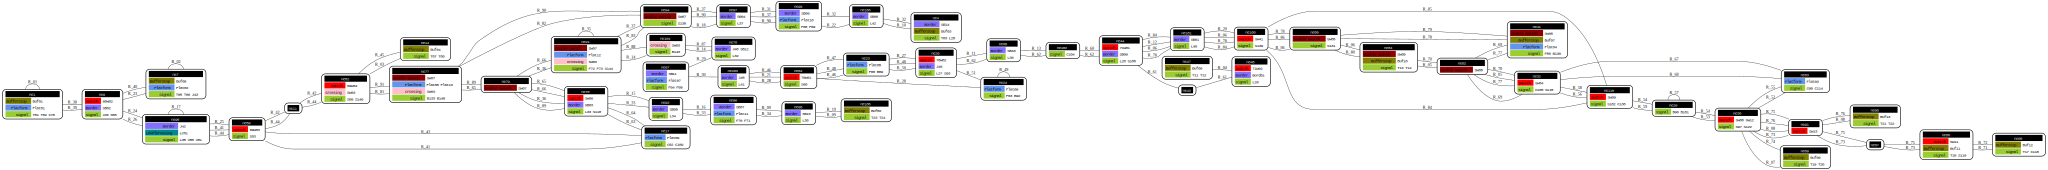
\includegraphics[origin = c, width=\textwidth]{Figuras/Graph_3}
		\centering\caption{Red de grafos generada por el RNA para el ejemplo 3.}
		\label{fig:EJ3_8}
	\end{figure}
	
	Cada nodo del grafo de la Figura \ref{fig:EJ3_8} corresponde a un \textit{netElement}. En cada nodo se listan todos los elementos ferroviarios contenidos por en \textit{netElement}. Las aristas del grafo son las rutas que los conectan. De esta manera, es posible detectar visualmente cualquier nodo aislado de la red o nodos que solo son accedidos en un sentido. Por ejemplo, si algún entre dos nodos no existe una cantidad par de rutas, entonces solamente se puede circular entre esos nodos en un solo sentido.
    \subsection{Señalamiento generado por el RNA}

    \lipsum[1]
    
    \begin{table}[H]
        {
        \caption{Tabla de enclavamiento del ejemplo 3 generada por el RNA (Rutas 1 a 15).}
        \label{Tab:tabla_generated_3_1}
        \centering
        \resizebox{1\textwidth}{!}{
            \begin{tabular}{ c c c c c c c }
                \hline	
                    Ruta & Inicio & Final & Cambio & Plataforma & Cruce & netElement\\	
                \hline
                    R$_{01}$ & T02 & C78 & - & Plat$_{01}$ & - & ne$_{1}$-ne$_{1}$\\
                    R$_{02}$ & T06 & J43 & - & Plat$_{02}$ & - & ne$_{7}$-ne$_{7}$\\
                    R$_{03}$ & T08 & P77 & 69W$_{04}^{N}$ & Plat$_{08}$ & - & ne$_{14}$-ne$_{77}$\\
                    R$_{04}$ & T10 & C100 & Sw$_{04}^{R}$ & Plat$_{04}$ & - & ne$_{41}$-ne$_{32}$\\
                    R$_{05}$ & T10 & S105 & Sw$_{41}^{R}$ & Plat$_{04}$ & - & ne$_{41}$-ne$_{44}$\\
                    R$_{06}$ & T12 & L29 & 71W$_{02}^{R}$ & - & - & ne$_{47}$-ne$_{48}$\\
                    R$_{07}$ & T14 & C100 & Sw$_{04}^{R}$ & - & - & ne$_{84}$-ne$_{32}$\\
                    R$_{08}$ & T14 & S105 & Sw$_{41}^{R}$ & - & - & ne$_{84}$-ne$_{44}$\\
                    R$_{09}$ & T20 & S97 & Sw$_{12}^{N}$ & - & - & ne$_{89}$-ne$_{30}$\\
                    R$_{10}$ & T22 & S97 & Sw$_{12}^{R}$+Sw$_{13}^{R}$ & - & - & ne$_{90}$-ne$_{30}$\\
                    R$_{11}$ & T24 & P70 & - & Plat$_{11}$ & - & ne$_{105}$-ne$_{96}$\\
                    R$_{12}$ & L25 & L42 & - & - & - & ne$_{4}$-ne$_{106}$\\
                    R$_{13}$ & L27 & L30 & - & - & - & ne$_{26}$-ne$_{65}$\\
                    R$_{14}$ & L28 & L40 & - & - & - & ne$_{44}$-ne$_{101}$\\
                    R$_{15}$ & L30 & C104 & - & - & - & ne$_{65}$-ne$_{102}$\\
                \hline
            \end{tabular}
        }
     }
    \end{table}

	\lipsum[1]
	
    \begin{table}[H]
        {
        \caption{Tabla de enclavamiento del ejemplo 3 generada por el RNA (Rutas 16 a 30).}
        \label{Tab:tabla_generated_3_2}
        \centering
        \resizebox{1\textwidth}{!}{
            \begin{tabular}{ c c c c c c c }
                \hline	
                    Ruta & Inicio & Final & Cambio & Plataforma & Cruce & netElement\\	
                \hline
                    R$_{16}$ & L32 & P73 & Sw$_{03}^{N}$ & - & - & ne$_{70}$-ne$_{21}$\\
                    R$_{17}$ & L33 & L34 & - & - & - & ne$_{78}$-ne$_{93}$\\
                    R$_{18}$ & L34 & P71 & - & Plat$_{11}$ & - & ne$_{93}$-ne$_{96}$\\
                    R$_{19}$ & L35 & X50 & - & - & - & ne$_{95}$-ne$_{95}$\\
                    R$_{20}$ & L37 & P76 & - & Plat$_{08}$ & - & ne$_{97}$-ne$_{77}$\\
                    R$_{21}$ & L37 & P72 & - & Plat$_{12}$ & - & ne$_{97}$-ne$_{21}$\\
                    R$_{22}$ & L38 & T23 & - & - & - & ne$_{98}$-ne$_{105}$\\
                    R$_{23}$ & L40 & S126 & - & - & - & ne$_{101}$-ne$_{100}$\\
                    R$_{24}$ & L41 & S90 & - & - & - & ne$_{103}$-ne$_{64}$\\
                    R$_{25}$ & L42 & P68 & - & Plat$_{10}$ & - & ne$_{106}$-ne$_{99}$\\
                    R$_{26}$ & J43 & J46 & 68W$_{02}^{R}$ & - & - & ne$_{7}$-ne$_{9}$\\
                    R$_{27}$ & J46 & L35 & - & - & - & ne$_{9}$-ne$_{95}$\\
                    R$_{28}$ & X50 & S83 & - & - & Lc01 & ne$_{95}$-ne$_{59}$\\
                    R$_{29}$ & X51 & S80 & - & - & Lc01 & ne$_{95}$-ne$_{9}$\\
                    R$_{30}$ & P60 & L27 & 70W$_{02}^{N}$ & - & - & ne$_{23}$-ne$_{26}$\\
                \hline
            \end{tabular}
        }
     }
    \end{table}

	\lipsum[1]
	
    \begin{table}[H]
        {
        \caption{Tabla de enclavamiento del ejemplo 3 generada por el RNA (Rutas 31 a 45).}
        \label{Tab:tabla_generated_3_3}
        \centering
        \resizebox{1\textwidth}{!}{
            \begin{tabular}{ c c c c c c c }
                \hline	
                    Ruta & Inicio & Final & Cambio & Plataforma & Cruce & netElement\\	
                \hline
                    R$_{31}$ & P63 & L41 & 70W$_{01}^{N}$ & - & - & ne$_{24}$-ne$_{103}$\\
                    R$_{32}$ & P64 & L32 & - & - & - & ne$_{67}$-ne$_{70}$\\
                    R$_{33}$ & P65 & L41 & - & - & - & ne$_{67}$-ne$_{103}$\\
                    R$_{34}$ & P68 & L37 & - & - & - & ne$_{99}$-ne$_{97}$\\
                    R$_{35}$ & P69 & T03 & - & - & - & ne$_{99}$-ne$_{4}$\\
                    R$_{36}$ & P70 & S110 & - & - & - & ne$_{96}$-ne$_{78}$\\
                    R$_{37}$ & P71 & L38 & - & - & - & ne$_{96}$-ne$_{98}$\\
                    R$_{38}$ & P72 & L32 & - & - & - & ne$_{21}$-ne$_{70}$\\
                    R$_{39}$ & P73 & L33 & Sw$_{06}^{R}$ & - & - & ne$_{21}$-ne$_{78}$\\ 
                    R$_{40}$ & P73 & P69 & - & Plat$_{10}$ & - & ne$_{21}$-ne$_{99}$\\
                    R$_{41}$ & P76 & S86 & - & - & - & ne$_{77}$-ne$_{52}$\\
                    R$_{42}$ & P77 & L33 & Sw$_{06}^{R}$ & - & - & ne$_{77}$-ne$_{78}$\\
                    R$_{43}$ & P77 & P69 &  & Plat$_{10}$ & - & ne$_{77}$-ne$_{99}$\\
                    R$_{44}$ & C78 & J46 & 68W$_{02}^{N}$ & - & - & ne$_{1}$-ne$_{9}$\\
                    R$_{45}$ & S80 & T01 & 68W$_{02}^{N}$ & Plat$_{01}$ & - & ne$_{9}$-ne$_{1}$\\
                \hline
            \end{tabular}
        }
     }
    \end{table}

	\lipsum[1]
	
    \begin{table}[H]
        {
        \caption{Tabla de enclavamiento del ejemplo 3 generada por el RNA (Rutas 46 a 60).}
        \label{Tab:tabla_generated_3_4}
        \centering
        \resizebox{1\textwidth}{!}{
            \begin{tabular}{ c c c c c c c }
                \hline	
                    Ruta & Inicio & Final & Cambio & Plataforma & Cruce & netElement\\	
                \hline
                    R$_{46}$ & S80 & T05 & 68W$_{02}^{R}$ & Plat$_{02}$ & - & ne$_{9}$-ne$_{7}$\\
                    R$_{47}$ & S82 & X51 & 69W$_{03}^{N}$ & - & - & ne$_{17}$-ne$_{95}$\\
                    R$_{48}$ & S83 & P77 & 69W$_{03}^{R}$+69W$_{04}^{R}$ & Plat$_{08}$ & - & ne$_{59}$-ne$_{77}$\\
                    R$_{49}$ & S83 & S109 & 69W$_{03}^{N}$ & Plat$_{09}$ & - & ne$_{59}$-ne$_{17}$\\
                    R$_{50}$ & S86 & X51 & 69W$_{03}^{R}$+69W$_{04}^{R}$ & - & - & ne$_{52}$-ne$_{95}$\\
                    R$_{51}$ & S86 & T07 & 69W$_{04}^{N}$ & - & - & ne$_{52}$-ne$_{14}$\\
                    R$_{52}$ & B89 & L41 & 70W$_{01}^{R}$ & Plat$_{05}$ & - & ne$_{23}$-ne$_{103}$\\
                    R$_{53}$ & S90 & P60 & 70W$_{01}^{R}$ & Plat$_{05}$ & - & ne$_{64}$-ne$_{23}$\\
                    R$_{54}$ & S90 & L27 & 70W$_{01}^{R}$+70W$_{02}^{N}$ & Plat$_{05}$ & - & ne$_{64}$-ne$_{26}$\\
                    R$_{55}$ & B92 & P63 & - & - & - & ne$_{24}$-ne$_{24}$\\
                    R$_{56}$ & S93 & B89 & 70W$_{02}^{N}$ & - & - & ne$_{26}$-ne$_{23}$\\
                    R$_{57}$ & S93 & P92 & 70W$_{02}^{R}$ & Plat$_{06}$ & - & ne$_{26}$-ne$_{24}$\\
                    R$_{58}$ & S95 & S119 & Sw$_{08}^{N}$ & - & - & ne$_{83}$-ne$_{30}$\\
                    R$_{59}$ & S96 & S119 & Sw$_{08}^{R}$ & - & - & ne$_{29}$-ne$_{30}$\\
                    R$_{60}$ & S97 & C124 & Sw$_{08}^{R}$+Sw$_{09}^{R}$ & - & - & ne$_{30}$-ne$_{110}$\\
                \hline
            \end{tabular}
        }
     }
    \end{table}
    
    \lipsum[1]
    
    \begin{table}[H]
        {
        \caption{Tabla de enclavamiento del ejemplo 3 generada por el RNA (Rutas 61 a 75).}
        \label{Tab:tabla_generated_3_5}
        \centering
        \resizebox{1\textwidth}{!}{
            \begin{tabular}{ c c c c c c c }
                \hline	
                    Ruta & Inicio & Final & Cambio & Plataforma & Cruce & netElement\\	
                \hline
                    R$_{61}$ & S97 & C112 & Sw$_{08}^{N}$ & Plat$_{03}$ & - & ne$_{30}$-ne$_{83}$\\
                    R$_{62}$ & C100 & S124 & Sw$_{09}^{N}$ & - & - & ne$_{32}$-ne$_{110}$\\
                    R$_{63}$ & B101 & S96 & - & - & - & ne$_{29}$-ne$_{29}$\\
                    R$_{64}$ & S102 & S113 & Sw$_{09}^{N}$ & - & - & ne$_{110}$-ne$_{32}$\\
                    R$_{65}$ & S102 & B101 & Sw$_{09}^{R}$ & - & - & ne$_{110}$-ne$_{29}$\\
                    R$_{66}$ & C104 & L28 & 71W$_{01}^{N}$ & - & - & ne$_{102}$-ne$_{44}$\\
                    R$_{67}$ & S105 & L29 & 71W$_{01}^{R}$+71W$_{02}^{N}$ & - & - & ne$_{44}$-ne$_{48}$\\
                    R$_{68}$ & S105 & S93 & 71W$_{01}^{N}$ & - & - & ne$_{44}$-ne$_{26}$\\
                    R$_{69}$ & C109 & L33 & Sw$_{06}^{N}$ & - & - & ne$_{17}$-ne$_{78}$\\
                    R$_{70}$ & S110 & S82 & Sw$_{06}^{N}$ & Plat$_{09}$ & - & ne$_{78}$-ne$_{17}$\\
                    R$_{71}$ & S110 & P76 & Sw$_{06}^{R}$ & Plat$_{08}$ & - & ne$_{78}$-ne$_{77}$\\
                    R$_{72}$ & S110 & P72 & Sw$_{06}^{R}$ & Plat$_{12}$ & - & ne$_{78}$-ne$_{21}$\\
                    R$_{73}$ & C112 & C100 & Sw$_{04}^{N}$ & - & - & ne$_{83}$-ne$_{32}$\\
                    R$_{74}$ & S113 & C95 & Sw$_{04}^{N}$ & Plat$_{03}$ & - & ne$_{32}$-ne$_{83}$\\
                    R$_{75}$ & S113 & P58 & Sw$_{04}^{R}$ & Plat$_{04}$ & - & ne$_{32}$-ne$_{41}$\\
                \hline
            \end{tabular}
        }
     }
    \end{table}
    
    \lipsum[1]
    
    \begin{table}[H]
        {
        \caption{Tabla de enclavamiento del ejemplo 3 generada por el RNA (Rutas 75 a 87).}
        \label{Tab:tabla_generated_3_6}
        \centering
        \resizebox{1\textwidth}{!}{
            \begin{tabular}{ c c c c c c c }
                \hline	
                    Ruta & Inicio & Final & Cambio & Plataforma & Cruce & netElement\\	
                \hline
                    R$_{76}$ & S113 & S13 & Sw$_{04}^{R}$ & - & - & ne$_{32}$-ne$_{84}$\\
                    R$_{77}$ & S115 & S15 & Sw$_{11}^{N}$ & - & - & ne$_{88}$-ne$_{86}$\\
                    R$_{78}$ & S116 & S17 & Sw$_{11}^{N}$ & - & - & ne$_{86}$-ne$_{88}$\\
                    R$_{79}$ & S116 & S97 & Sw$_{11}^{R}$+Sw$_{12}^{R}$+Sw$_{13}^{N}$ & - & - & ne$_{86}$-ne$_{30}$\\
                    R$_{80}$ & S119 & S19 & Sw$_{12}^{N}$ & - & - & ne$_{30}$-ne$_{89}$\\
                    R$_{81}$ & S119 & S15 & Sw$_{11}^{R}$+Sw$_{12}^{R}$+Sw$_{13}^{N}$ & - & - & ne$_{30}$-ne$_{86}$\\
                    R$_{82}$ & S119 & S21 & Sw$_{12}^{R}$+Sw$_{13}^{R}$ & - & - & ne$_{30}$-ne$_{90}$\\
                    R$_{83}$ & S124 & S105 & Sw$_{41}^{N}$ & - & - & ne$_{110}$-ne$_{44}$\\
                    R$_{84}$ & S125 & S58 & - & Plat$_{04}$ & - & ne$_{85}$-ne$_{41}$\\
                    R$_{85}$ & S125 & S13 & - & - & - & ne$_{85}$-ne$_{84}$\\
                    R$_{86}$ & S126 & S102 & Sw$_{41}^{N}$ & - & - & ne$_{100}$-ne$_{110}$\\
                    R$_{87}$ & S126 & S125 & Sw$_{41}^{R}$ & - & - & ne$_{100}$-ne$_{85}$\\
                \hline
            \end{tabular}
        }
     }
    \end{table}
    
    \lipsum[1]
    \section{Validación del sistema}

	La validación de las rutas de la tabla de enclavamientos es realizada por el RNA aplicando el Algoritmo \ref{alg:interlocking_tables}, explicado en la Sección \ref{sec:validar_tabla}. Las 33 rutas del señalamiento original (Tabla \ref{Tab:tabla_original_3}) tienen 33 rutas equivalentes en el señalamiento generado por el RNA (Tabla \ref{Tab:tabla_generated_3_1}, \ref{Tab:tabla_generated_3_2}, \ref{Tab:tabla_generated_3_3}, \ref{Tab:tabla_generated_3_4}, \ref{Tab:tabla_generated_3_5}, \ref{Tab:tabla_generated_3_6}), tal como se puede visualizar en la Tabla \ref{Tab:tabla_validation_3_1}, generada automáticamente por el RNA. % y Tabla \ref{Tab:tabla_validation_3_2}, generada automáticamente por el RNA.

    \begin{table}[H]
        {
        \caption{Equivalencias entre las rutas originales y las generadas por el RNA.}
        \label{Tab:tabla_validation_3_1}
        \centering
        %\small
            %\centering
            \begin{center}
            \resizebox{0.9\textwidth}{!}{
            \begin{tabular}{ c c c c }
                \hline	
                    Original & Señales & RNA & Señales \\	
                \hline
                    R$_{01}$ & 68N1-69Va & R$_{23}$+R$_{24}$ & J$_{43}$-L$_{35}$\\
                    R$_{02}$ & 68N2-69Va & R$_{38}$+R$_{24}$ & C$_{78}$-L$_{35}$\\
                    R$_{03}$ & 69Va-69A & R$_{25}$ & X$_{50}$-S$_{83}$\\
                    R$_{04}$ & 69A-69N2 & R$_{43}$ & S$_{83}$-S$_{109}$\\
                    R$_{05}$ & 69A-69N3 & R$_{42}$+R$_{91}$ & S$_{83}$-B$_{145}$\\
                    R$_{06}$ & 69P2-68F & R$_{41}$+R$_{26}$ & S$_{82}$-S$_{80}$\\
                    R$_{07}$ & 69B2-69P2 & R$_{64}$ & S$_{110}$-S$_{82}$\\
                    R$_{08}$ & 69B2-69P3 & R$_{65}$ & S$_{110}$-B$_{133}$\\
                    R$_{09}$ & 69B2-69P1 & R$_{66}$ & S$_{110}$-P$_{72}$\\
                    R$_{10}$ & 69C-69N1 & R$_{14}$ & L$_{32}$-T$_{73}$\\
                    R$_{11}$ & 69Vc1-69C & R$_{88}$+R$_{87}$ & S$_{144}$-L$_{32}$\\
                    R$_{12}$ & 69Vc-69Vc1 & R$_{29}$ & P$_{64}$-L$_{32}$\\
                    R$_{13}$ & 70Va-70A & R$_{21}$ & L$_{41}$-S$_{90}$\\
                    R$_{14}$ & 70N2-69Vc & R$_{27}$ & P$_{60}$-L$_{27}$\\
                    R$_{15}$ & 70N1-69Vc & R$_{28}$ & P$_{63}$-L$_{41}$\\
                    R$_{16}$ & 70P1-72Va & R$_{28}$+R$_{21}$+R$_{48}$+R$_{11}$+R$_{13}$+R$_{60}$ & P$_{63}$-L$_{28}$\\
    %            \hline
    %        \end{tabular}
    %        }
    %        \end{center}
    %    }    
    %\end{table}

	%\lipsum[1]
	
    %\begin{table}[H]
    %    {
    %    \caption{Equivalencias entre las rutas originales y las generadas por el RNA (Rutas 17 a 33).}
    %    \label{Tab:tabla_validation_3_2}
    %    \centering
        %\small
            %\centering
   %         \begin{center}
   %         \resizebox{0.8\textwidth}{!}{
   %         \begin{tabular}{ c c c c }
   %             \hline	
   %                 Original & Señales & RNA & Señales \\	
   %             \hline
                    R$_{17}$ & 70P2-72Va & R$_{27}$+R$_{11}$+R$_{13}$+R$_{60}$ & P$_{60}$-L$_{28}$\\
                    R$_{18}$ & 70B-70N2 & R$_{50}$ & S$_{93}$-B$_{89}$\\
                    R$_{19}$ & 70B-70N1 & R$_{51}$ & S$_{93}$-P$_{92}$\\
                    R$_{20}$ & 70A-70P1 & R$_{48}$+R$_{51}$ & S$_{90}$-P$_{92}$\\
                    R$_{21}$ & 70A-70P2 & R$_{47}$ & S$_{90}$-P$_{60}$\\
                    R$_{22}$ & 69W04Y-69N3 & R$_{03}$+R$_{91}$ & T$_{08}$-B$_{145}$\\
                    R$_{23}$ & 72Va-72A & R$_{12}$+R$_{20}$ & L$_{28}$-S$_{139}$\\
                    R$_{24}$ & 721-S01 & R$_{67}$ & C$_{114}$-C$_{100}$\\
                    R$_{25}$ & 723b-S01 & R$_{77}$ & B$_{130}$-C$_{100}$\\
                    R$_{26}$ & 723b-72B & R$_{78}$+R$_{12}$+R$_{20}$ & B$_{130}$-S$_{139}$\\
                    R$_{27}$ & 722-72B & R$_{53}$+R$_{54}$+R$_{84}$+R$_{12}$+R$_{20}$ & S$_{96}$-S$_{122}$\\
                    R$_{28}$ & S01-72B & R$_{70}$+R$_{06}$+R$_{12}$+R$_{20}$ & S$_{113}$-S$_{122}$\\
                    R$_{29}$ & 69B1-69P3 & R$_{82}$ & S$_{135}$-B$_{133}$\\
                    R$_{30}$ & 69B1-69P1 & R$_{83}$ & S$_{135}$-P$_{72}$\\
                    R$_{31}$ & 72B-70B & R$_{85}$+R$_{84}$+R$_{62}$ & S$_{139}$-S$_{93}$\\
                    R$_{32}$ & 69P3-68F & R$_{81}$+R$_{44}$+R$_{26}$ &B$_{133}$-S$_{80}$\\
                    R$_{33}$ & 69P1-70Va & R$_{36}$ & P$_{73}$-L$_{33}$\\
                \hline
            \end{tabular}
            }
            \end{center}
        }    
    \end{table}
    
    Las rutas R1, R2, R5, R6, R11, R16, R17, R20, R22, R23, R26, R27, R28, R31 y R32 del señalamiento original fueron divididas en rutas mas pequeñas en el señalamiento generado por el RNA. La razón para dividir la ruta depende de cada caso, tal sea por su longitud y/o por abarcar diversos elementos ferroviarios. Por ejemplo, la ruta R32 fue dividida por ambos motivos: es muy extensa y atraviesa un cambio de vías en tijeras, dos cambios de vías simples, un cruce de vías y una plataforma. Las rutas producto de particionar R32 (R81, R44 y R26 del nuevo señalamiento) añaden paradas luego de cruzar el cambio de vías en tijeras y antes del cruce de vías, incrementando la seguridad y flexibilidad en la logística de la red. Un análisis similar puede hacerse con las demás rutas particionadas.
    
    De las 91 rutas generadas por el RNA, 29 son particiones de rutas originales, por lo que 62 de ellas están relacionadas de alguna manera a las 33 rutas originales. Las 29 rutas restantes corresponden a la protección de los 12 finales de vía absolutos y al único final de vía relativo, además de las señales añadidas para poder operar las playas de maniobras que se encontraban sin señalamiento.
    
    Para finalizar, el RNA comprueba los principios de señalamiento ferroviario explicados en la Sección \label{sec:validar_principios}, aplicando los algoritmos indicados, de los cuáles se obtuvieron los siguientes resultados:
    
    \begin{itemize}
    	\item Principio de autoridad (Algoritmo \ref{alg:ppio_autoridad}): cobertura del 100\% de los \textit{netElements}.
    	\item Principio de claridad (Algoritmo \ref{alg:ppio_claridad}): rutas 100\% independientes.
    	\item Principio de anticipación (Algoritmo \ref{alg:ppio_anticipacion}): cobertura del 100\% de los puntos críticos.
    	\item Principio de granularidad (Algoritmo \ref{alg:ppio_granularidad}): 100\% de rutas divididas a su mínima expresión.
    	\item Principio de terminalidad (Algoritmo \ref{alg:ppio_terminalidad}): 100\% de finales de vías protegidos.
    	\item Principio de infraestructura (Algoritmo \ref{alg:ppio_infraestructura}): 100\% de infraestructura protegida.
    	\item Principio de no bloqueo (Algoritmo \ref{alg:ppio_nobloqueo}): 100\% de cambios de vías protegidos.
    \end{itemize}	
    \subsection{Sistema generado por el ACG}

En base a la red de grafos, ilustrada en la Figura \ref{fig:EJ3_8}, el ACG determinó la siguiente cantidad de elementos, tal puede visualizarse en el Código \ref{lst:EJ3_8}.

\begin{lstlisting}[language = {}, caption = Cantidad de elementos a implementar por el ACG, label = {lst:EJ3_8}]
n_netElements:53
n_switch:15
n_doubleSwitch:2
n_borders:18
n_buffers:12
n_levelCrossings:1
n_platforms:13
n_scissorCrossings:1
n_signals:82
N : 329
M : 276
\end{lstlisting}

El código VHDL generado por el ACG es importado en un proyecto de Vivado, donde es sintetizado e implementado para generar el bitstream que será utilizado para programar la FPGA. La cantidad de elementos de la FPGA utilizados por el sistema post-síntesis y post-implementación, así como el porcentaje de uso de la plataforma, son detallados en la Tabla \ref{Tab:tabla_ACG_3}.

\begin{table}[H]
	{
		\caption{Síntesis e implementación del ejemplo 3 generado por el ACG.}
		\label{Tab:tabla_ACG_3}
		\centering
		%\small
		%\centering
		\begin{center}
			\resizebox{0.7\textwidth}{!}{
				\begin{tabular}{ c c c c }
					\hline	
					Recursos & Síntesis & Implementación & Uso \\	
					\hline
					LUT & 13802 & 137873 & 25.94-25.91\%\\
					FF & 17321 & 17321 & 16.28\%\\
					IO & 16 & 16 & 12.80\%\\
					BUFG & 1 & 1 & 3.13\%\\
					\hline
				\end{tabular}
			}
		\end{center}
	}    
\end{table}

En este ejemplo, la cantidad de recursos utilizados es baja y el tiempo de sintetización e implementación es de 1 minuto con 43 segundos y 1 minuto con 20 segundos respectivamente.
    
	%\section{Ejemplo 4}
 
    \subsection{Topología ferroviaria original}

\lipsum[2]


\begin{figure}[H]
	\centering
	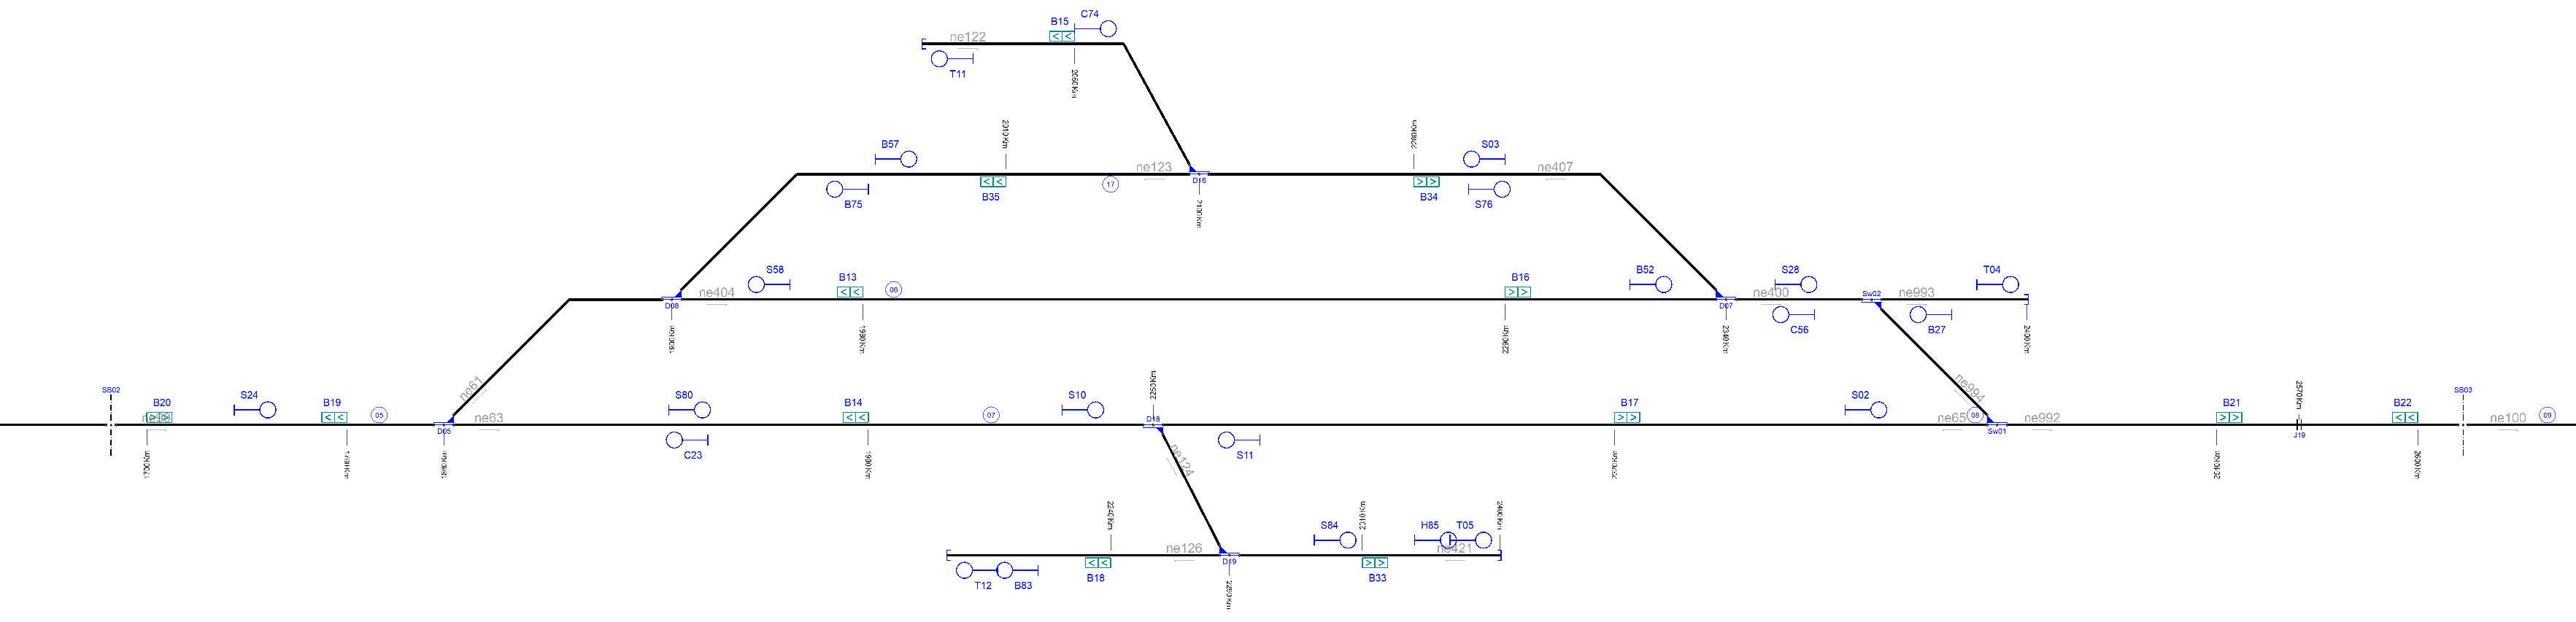
\includegraphics[width=1\textwidth]{resultados-obtenidos/ejemplo4/images/4_original.png}
	\centering\caption{Señalamiento original del ejemplo 4.}
	%\label{fig:LC_P2}
\end{figure}

\lipsum[2]

\begin{figure}[H]
	\centering
	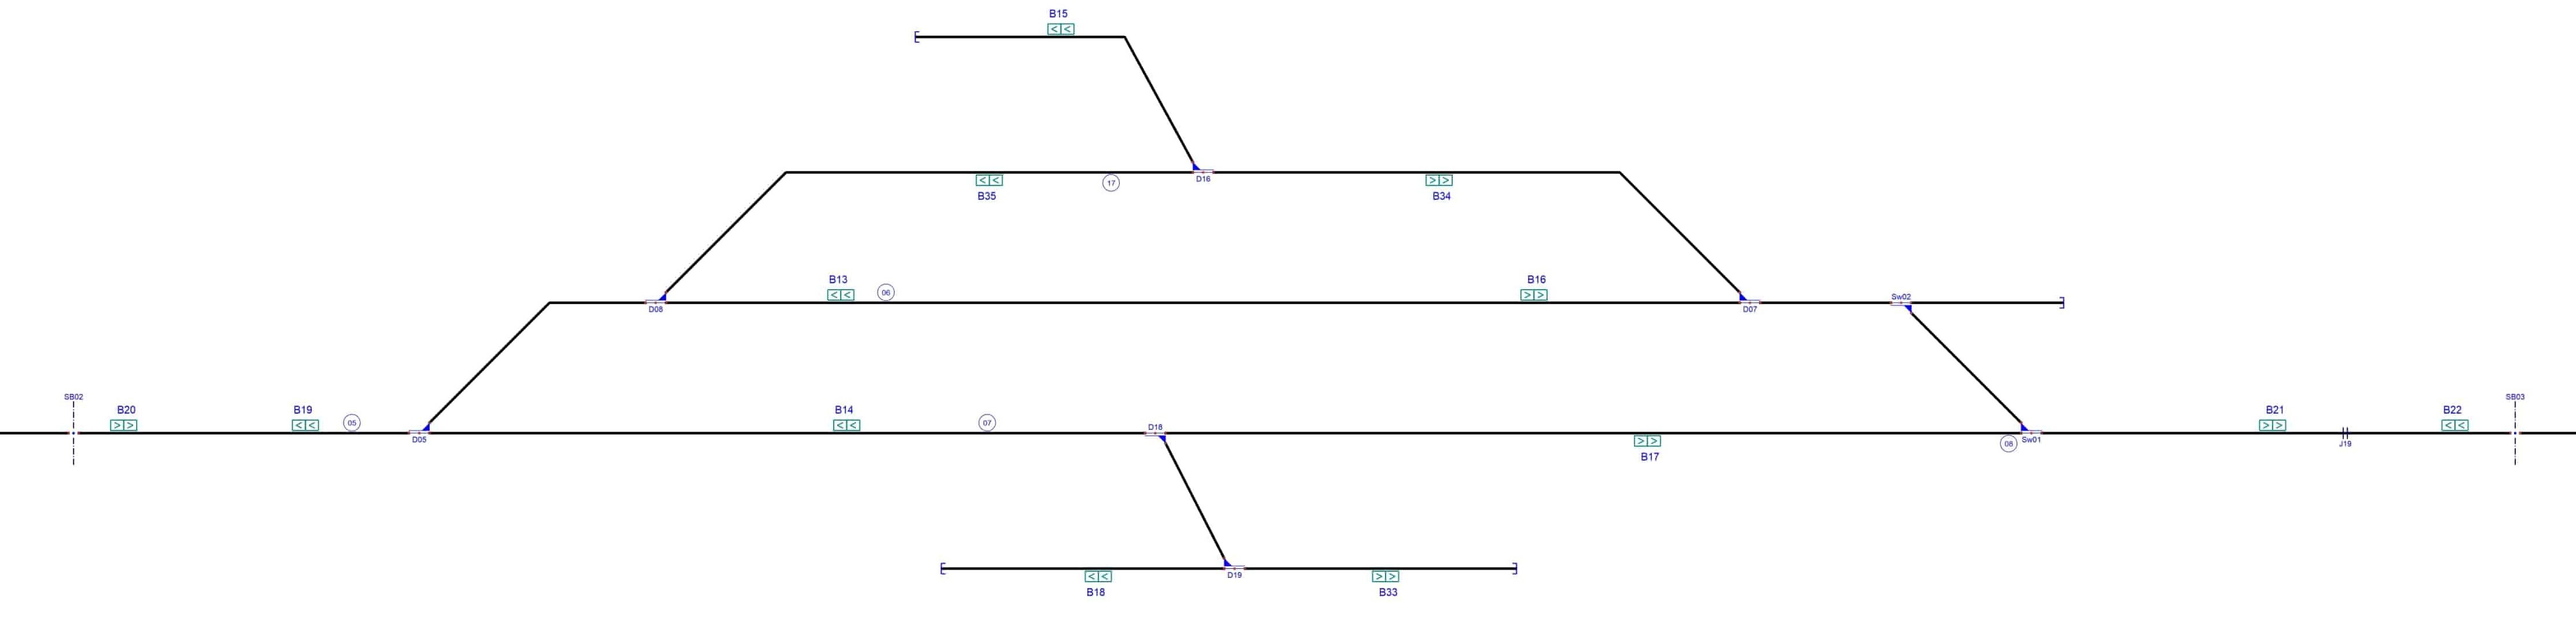
\includegraphics[width=1\textwidth]{resultados-obtenidos/ejemplo4/images/4_empty.png}
	\centering\caption{Topología ferroviaria del ejemplo 4 sin señalamiento.}
	%\label{fig:LC_P2}
\end{figure}

\lipsum[2]

    \section{Señalamiento original}

    El señalamiento original, ilustrado en la Figura \ref{fig:EJ4_2} incluye 71 señales y es demasiado extenso para describirlo en detalle. El mismo incluye señales de parada próximas a los finales de vías absolutos, señales de partida en las plataformas, señales de protección antes de cada paso a nivel  señales de maniobras antes de converger en una vía principal y señales múltiples para cambios de vías divergentes.
    
    \begin{figure}[H]
    	\centering
    	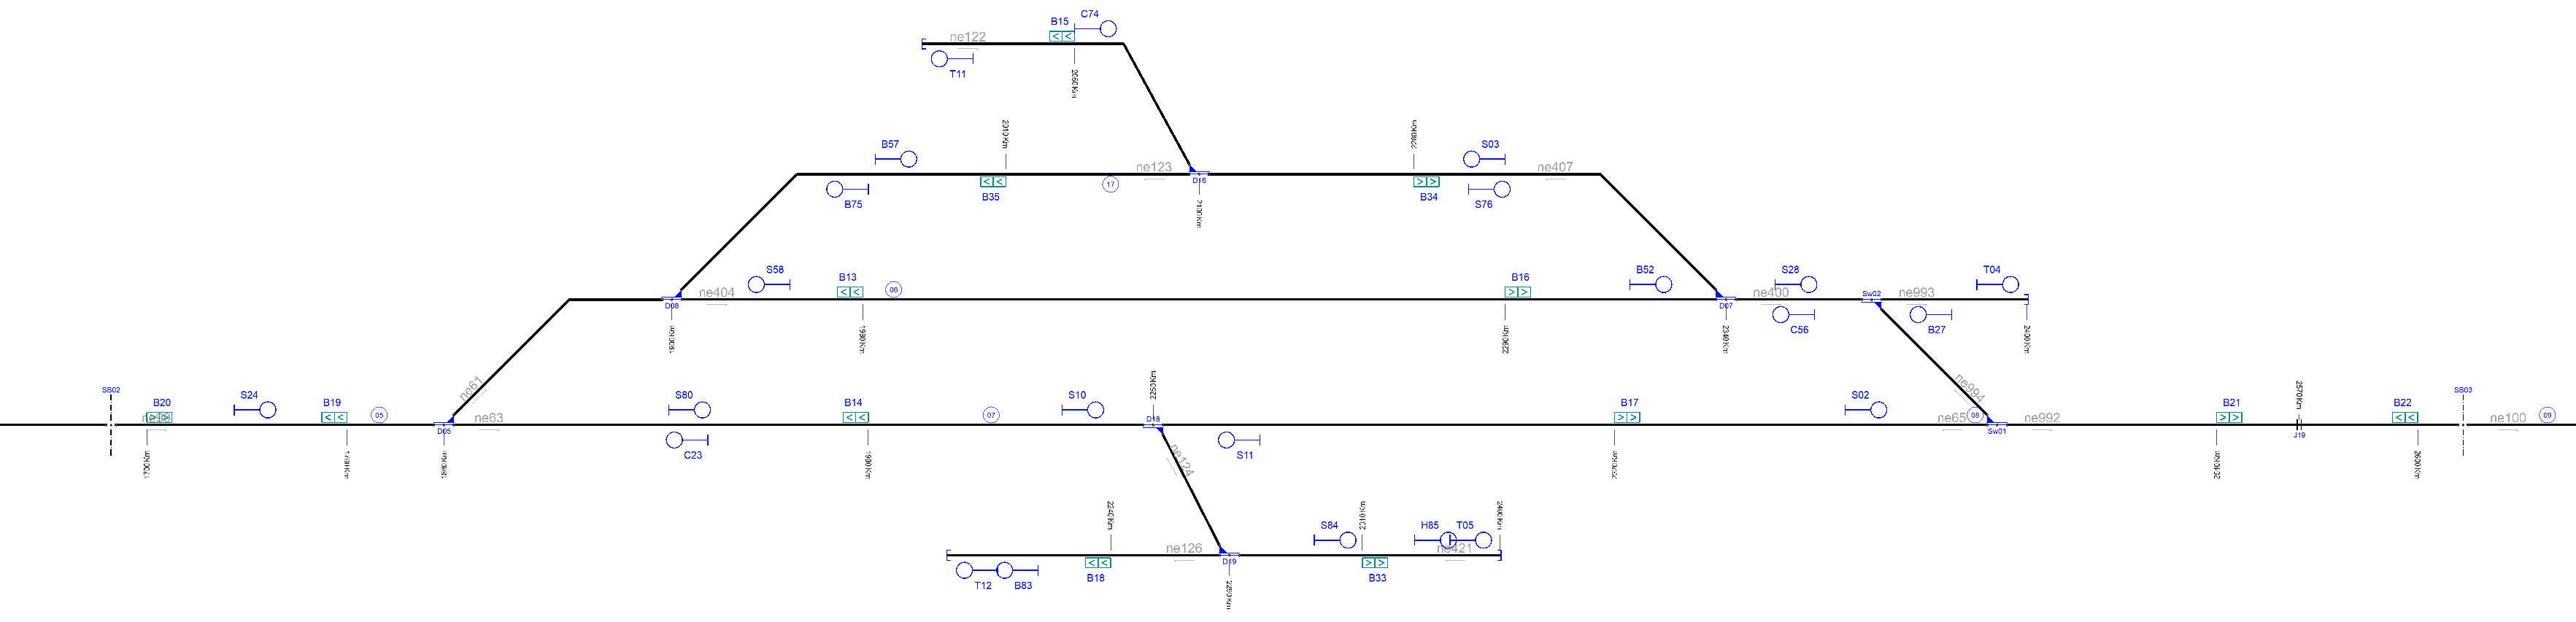
\includegraphics[width=1\textwidth]{resultados-obtenidos/ejemplo4/images/4_original.png}
    	\centering\caption{Señalamiento original del ejemplo 4.}
    	\label{fig:EJ4_2}
    \end{figure}
    
    Estas señales permiten definir hasta un máximo de 77 rutas, las cuales no pueden ser detalladas en una única tabla, por lo que serán particionadas en las Tablas \ref{Tab:tabla_original_4_1}, \ref{Tab:tabla_original_4_2}, \ref{Tab:tabla_original_4_3}, \ref{Tab:tabla_original_4_4} y \ref{Tab:tabla_original_4_5}. En una primera inspección, se puede comprobar que el señalamiento de este ejemplo no es tan complejo como el del ejemplo 3, si es el mas extenso que se analizará en este trabajo.    
    
    \begin{table}[H]
        {
        \caption{Tabla de enclavamiento original del ejemplo 4 (Rutas 1 a 15).}
        \label{Tab:tabla_original_4_1}
        \centering
        \resizebox{1\textwidth}{!}{
            \begin{tabular}{ c c c c c c c }
                \hline	
                    Ruta & Inicio & Final & Cambio & Plataforma & Cruce & netElement \\	
                \hline
                    R$_{01}$ & S$_{15}$ & S$_{24}$ & - & - & Lc$_{02}$ & ne$_{98}$-ne$_{99}$\\
                    R$_{02}$ & S$_{16}$ & S$_{67}$ & Sw$_{04}^{N}$ & - & Lc$_{02}$ & ne$_{98}$-ne$_{292}$\\
                    R$_{03}$ & S$_{16}$ & S$_{43}$ & Sw$_{04}^{R}$ & - & Lc$_{02}$ & ne$_{98}$-ne$_{297}$\\
                    R$_{04}$ & S$_{19}$ & S$_{32}$ & - & - & Lc$_{06}$ & ne$_{100}$-ne$_{101}$\\
                    R$_{05}$ & S$_{20}$ & S$_{11}$ & Sw$_{01}^{N}$ & - & Lc$_{06}$ & ne$_{100}$-ne$_{65}$\\
                    R$_{06}$ & S$_{20}$ & S$_{56}$ & Sw$_{01}^{R}$ & - & Lc$_{06}$ & ne$_{100}$-ne$_{400}$\\
                    R$_{07}$ & S$_{23}$ & S$_{16}$ & - & - & - & ne$_{63}$-ne$_{98}$\\
                    R$_{08}$ & S$_{24}$ & S$_{80}$ & D$_{05}^{N}$ & - & - & ne$_{99}$-ne$_{63}$\\
                    R$_{09}$ & S$_{24}$ & S$_{52}$ & D$_{05}^{R}$-D$_{08}^{N}$ & - & - & ne$_{99}$-ne$_{404}$\\
                    R$_{10}$ & S$_{24}$ & S$_{57}$ & D$_{05}^{R}$-D$_{08}^{R}$ & - & - & ne$_{99}$-ne$_{123}$\\
                    R$_{11}$ & S$_{27}$ & S$_{56}$ & - & - & - & ne$_{993}$-ne$_{400}$\\
                    R$_{12}$ & S$_{28}$ & S$_{04}$ & Sw$_{02}^{N}$ & - & - & ne$_{400}$-ne$_{384}$\\
                    R$_{13}$ & S$_{28}$ & S$_{19}$ & Sw$_{02}^{R}$ & - & Lc$_{05}$ & ne$_{400}$-ne$_{100}$\\
                    R$_{14}$ & S$_{31}$ & S$_{20}$ & - & - & - & ne$_{912}$-ne$_{100}$\\
                    R$_{15}$ & S$_{32}$ & S$_{91}$ & D$_{09}^{N}$ & - & - & ne$_{101}$-ne$_{912}$\\    
                \hline
            \end{tabular}
        }
     }
    \end{table}

	%\lipsum[1]
	
    \begin{table}[H]
        {
        \caption{Tabla de enclavamiento original del ejemplo 4 (Rutas 16 a 30).}
        \label{Tab:tabla_original_4_2}
        \centering
        \resizebox{1\textwidth}{!}{
            \begin{tabular}{ c c c c c c c }
                \hline	
                    Ruta & Inicio & Final & Cambio & Plataforma & Cruce & netElement \\	
                \hline
                    R$_{16}$ & S$_{32}$ & S$_{59}$ & D$_{09}^{R}$-D$_{10}^{N}$ & - & - & ne$_{101}$-ne$_{130}$\\
                    R$_{17}$ & S$_{32}$ & S$_{60}$ & D$_{09}^{R}$-D$_{10}^{R}$ & - & - & ne$_{101}$-ne$_{135}$\\
                    R$_{18}$ & S$_{35}$ & S$_{01}$ & - & - & - & ne$_{290}$-ne$_{130}$\\
                    R$_{19}$ & S$_{39}$ & S$_{43}$ & - & - & - & ne$_{995}$-ne$_{297}$\\
                    R$_{20}$ & S$_{44}$ & S$_{04}$ & - & - & - & ne$_{110}$-ne$_{384}$\\
                    R$_{21}$ & S$_{45}$ & S$_{01}$ & - & - & - & ne$_{295}$-ne$_{130}$\\
                    R$_{22}$ & S$_{46}$ & S$_{63}$ & Sw$_{02}^{N}$ & - & - & ne$_{384}$-ne$_{110}$\\
                    R$_{23}$ & S$_{46}$ & S$_{09}$ & Sw$_{02}^{R}$ & - & - & ne$_{384}$-ne$_{292}$\\
                    R$_{24}$ & S$_{47}$ & S$_{40}$ & - & - & - & ne$_{295}$-ne$_{297}$\\
                    R$_{25}$ & S$_{52}$ & S$_{28}$ & - & - & - & ne$_{404}$-ne$_{400}$\\
                    R$_{26}$ & S$_{56}$ & S$_{58}$ & D$_{07}^{N}$ & - & - & ne$_{400}$-ne$_{404}$\\
                    R$_{27}$ & S$_{56}$ & S$_{03}$ & D$_{07}^{R}$ & - & - & ne$_{400}$-ne$_{407}$\\
                    R$_{28}$ & S$_{57}$ & S$_{76}$ & - & - & - & ne$_{123}$-ne$_{407}$\\
                    R$_{29}$ & S$_{58}$ & S$_{16}$ & - & - & - & ne$_{404}$-ne$_{98}$\\
                    R$_{30}$ & S$_{59}$ & S$_{87}$ & D$_{12}^{T}$ & - & - & ne$_{130}$-ne$_{114}$\\
                \hline
            \end{tabular}
        }
     }
    \end{table}

	%\lipsum[1]
	
    \begin{table}[H]
        {
        \caption{Tabla de enclavamiento original del ejemplo 4 (Rutas 31 a 45).}
        \label{Tab:tabla_original_4_3}
        \centering
        \resizebox{1\textwidth}{!}{
            \begin{tabular}{ c c c c c c c }
                \hline	
                    Ruta & Inicio & Final & Cambio & Plataforma & Cruce & netElement \\	
                \hline
                    R$_{31}$ & S$_{59}$ & S$_{06}$ & D$_{12}^{S}$ & - & - & ne$_{130}$-ne$_{377}$\\
                    R$_{32}$ & S$_{60}$ & S$_{99}$ & - & - & - & ne$_{135}$-ne$_{127}$\\
                    R$_{33}$ & S$_{62}$ & S$_{04}$ & - & - & - & ne$_{104}$-ne$_{384}$\\
                    R$_{34}$ & S$_{63}$ & S$_{01}$ & - & - & - & ne$_{110}$-ne$_{130}$\\
                    R$_{35}$ & S$_{67}$ & S$_{09}$ & - & - & - & ne$_{292}$-ne$_{292}$\\
                    R$_{36}$ & S$_{68}$ & S$_{08}$ & - & - & - & ne$_{290}$-ne$_{290}$\\
                    R$_{37}$ & S$_{74}$ & S$_{76}$ & - & - & - & ne$_{122}$-ne$_{407}$\\
                    R$_{38}$ & S$_{75}$ & S$_{16}$ & - & - & - & ne$_{123}$-ne$_{98}$\\
                    R$_{39}$ & S$_{76}$ & S$_{28}$ & - & - & - & ne$_{407}$-ne$_{400}$\\
                    R$_{40}$ & S$_{80}$ & S$_{10}$ & - & - & - & ne$_{63}$-ne$_{63}$\\
                    R$_{41}$ & S$_{83}$ & S$_{12}$ & - & - & - & ne$_{126}$-ne$_{126}$\\
                    R$_{42}$ & S$_{84}$ & S$_{85}$ & - & - & - & ne$_{421}$-ne$_{421}$\\
                    R$_{43}$ & S$_{85}$ & S$_{05}$ & - & - & - & ne$_{421}$-ne$_{421}$\\
                    R$_{44}$ & S$_{86}$ & S$_{87}$ & - & - & - & ne$_{132}$-ne$_{114}$\\
                    R$_{45}$ & S$_{87}$ & S$_{08}$ & - & - & - & ne$_{114}$-ne$_{290}$\\
                \hline
            \end{tabular}
        }
     }
    \end{table}

	%\lipsum[1]
	
    \begin{table}[H]
        {
        \caption{Tabla de enclavamiento original del ejemplo 4 (Rutas 46 a 160).}
        \label{Tab:tabla_original_4_4}
        \centering
        \resizebox{1\textwidth}{!}{
            \begin{tabular}{ c c c c c c c }
                \hline	
                    Ruta & Inicio & Final & Cambio & Plataforma & Cruce & netElement \\	
                \hline
                    R$_{46}$ & S$_{89}$ & S$_{31}$ & - & - & - & ne$_{132}$-ne$_{912}$\\
                    R$_{47}$ & S$_{90}$ & S$_{89}$ & - & - & - & ne$_{132}$-ne$_{132}$\\
                    R$_{48}$ & S$_{91}$ & S$_{93}$ & - & - & - & ne$_{912}$-ne$_{912}$\\
                    R$_{49}$ & S$_{93}$ & S$_{86}$ & D$_{20}^{N}$ & - & - & ne$_{912}$-ne$_{132}$\\
                    R$_{50}$ & S$_{93}$ & S$_{95}$ & D$_{20}^{R}$ & - & - & ne$_{912}$-ne$_{465}$\\
                    R$_{51}$ & S$_{94}$ & S$_{13}$ & - & - & - & ne$_{133}$-ne$_{133}$\\
                    R$_{52}$ & S$_{95}$ & S$_{96}$ & - & - & - & ne$_{465}$-ne$_{465}$\\
                    R$_{53}$ & S$_{96}$ & S$_{07}$ & - & - & - & ne$_{465}$-ne$_{991}$\\
                    R$_{54}$ & S$_{97}$ & S$_{99}$ & - & - & - & ne$_{134}$-ne$_{127}$\\
                    R$_{55}$ & S$_{98}$ & S$_{20}$ & - & - & - & ne$_{135}$-ne$_{100}$\\
                    R$_{56}$ & S$_{99}$ & S$_{87}$ & D$_{12}^{S}$ & - & - & ne$_{127}$-ne$_{114}$\\
                    R$_{57}$ & S$_{99}$ & S$_{06}$ & D$_{12}^{T}$ & - & - & ne$_{127}$-ne$_{377}$\\
                    R$_{58}$ & S$_{40}$ & S$_{02}$ & Sw$_{03}^{N}$ & - & - & ne$_{297}$-ne$_{65}$\\
                    R$_{59}$ & S$_{40}$ & S$_{15}$ & Sw$_{03}^{R}$ & - & - & ne$_{297}$-ne$_{98}$\\
                    R$_{60}$ & S$_{43}$ & S$_{45}$ & D$_{04}^{N}$ &- & - & ne$_{297}$-ne$_{295}$\\
                \hline
            \end{tabular}
        }
     }
    \end{table}
    
    %\lipsum[1]
    
    \begin{table}[H]
        {
        \caption{Tabla de enclavamiento original del ejemplo 4 (Rutas 61 a 76).}
        \label{Tab:tabla_original_4_5}
        \centering
        \resizebox{1\textwidth}{!}{
            \begin{tabular}{ c c c c c c c }
                \hline	
                    Ruta & Inicio & Final & Cambio & Plataforma & Cruce & netElement \\	
                \hline
                    R$_{61}$ & S$_{43}$ & S$_{46}$ & D$_{04}^{R}$ & - & - & ne$_{297}$-ne$_{384}$\\
                    R$_{62}$ & S$_{01}$ & S$_{20}$ & - & - & - & ne$_{130}$-ne$_{100}$\\
                    R$_{63}$ & S$_{02}$ & S$_{19}$ & - & - & Lc$_{05}$ & ne$_{65}$-ne$_{100}$\\
                    R$_{64}$ & S$_{03}$ & S$_{75}$ & D$_{16}^{N}$ & - & - & ne$_{407}$-ne$_{123}$\\
                    R$_{65}$ & S$_{03}$ & S$_{11}$ & D$_{16}^{R}$ & - & - & ne$_{407}$-ne$_{65}$\\
                    R$_{66}$ & S$_{04}$ & S$_{40}$ & - & - & - & ne$_{384}$-ne$_{297}$\\
                    R$_{67}$ & S$_{06}$ & S$_{10}$ & D$_{15}^{N}$ & - & - & ne$_{377}$-ne$_{63}$\\
                    R$_{68}$ & S$_{06}$ & S$_{35}$ & D$_{15}^{R}$ & - & - & ne$_{377}$-ne$_{290}$\\
                    R$_{69}$ & S$_{07}$ & S$_{68}$ & D$_{01}^{N}$ & - & - & ne$_{991}$-ne$_{290}$\\
                    R$_{70}$ & S$_{07}$ & S$_{47}$ & D$_{01}^{R}$-D$_{03}^{N}$ & - & - & ne$_{991}$-ne$_{295}$\\
                    R$_{71}$ & S$_{07}$ & S$_{44}$ & D$_{01}^{R}$-D$_{03}^{R}$ & - & - & ne$_{991}$-ne$_{110}$\\
                    R$_{72}$ & S$_{08}$ & S$_{15}$ & D$_{14}^{N}$ & - & - & ne$_{290}$-ne$_{98}$\\
                    R$_{73}$ & S$_{08}$ & S$_{03}$ & D$_{14}^{R}$ & - & - & ne$_{290}$-ne$_{407}$\\
                    R$_{74}$ & S$_{09}$ & S$_{35}$ & - & - & - & ne$_{292}$-ne$_{290}$\\
                    R$_{75}$ & S$_{10}$ & S$_{02}$ & D$_{18}^{N}$ & - & - & ne$_{63}$-ne$_{65}$\\
                    R$_{76}$ & S$_{10}$ & S$_{84}$ & D$_{18}^{R}$ & - & - & ne$_{63}$-ne$_{421}$\\
                    R$_{77}$ & S$_{11}$ & S$_{23}$ & - & - & - & ne$_{65}$-ne$_{63}$\\
                \hline
            \end{tabular}
        }
     }
    \end{table}
    
    Algunas rutas abarcan mas de un \textit{netElement}, como por ejemplo la ruta R75 que comienza en la señal S10 y finaliza en la señal S02, atravesando los \textit{netElements} ne63 y ne65, utilizando el cambio de vías D18 en posición reversa.
    \section{Generación de señalamiento paso a paso}

Inicialmente, el RNA ejecuta el Algoritmo \ref{alg:graph_network} (ver Sección \ref{sec:grafos}) para detectar todos los \textit{netElements}, sus coordenadas iniciales y finales en la topología, y el sentido en el que fueron definidas. Al concluir el Algoritmo \ref{alg:graph_network}, el RNA ejecuta el Algoritmo \ref{alg:connectedness} (ver Sección \ref{sec:grafos}) para analizar la conexidad de la red. El resultado obtenido se muestra en el Código \ref{lst:EJ4_1}, donde se describen las coordenadas de cada \textit{netElement} y se confirma que la red es conexa.

\begin{lstlisting}[language = {}, tabsize=4, basicstyle=\footnotesize\ttfamily, showspaces=false, showstringspaces=false, caption = Detección de \textit{netElements} por parte del RNA , label = {lst:EJ4_1}]
###### Starting Railway Network Analyzer #####
Reading .railML file
Creating railML object
Analyzing railML object
Analyzing graph
ne991 [-1064, 0] [-2322, 0] <<
ne61 [4350, 0] [4804, 250] >> 
ne63 [4350, 0] [5763, 0] >>
ne65 [7444, 0] [5763, 0] <<
ne910 [11254, 0] [11822, 250] >>
ne912 [11254, 0] [13111, 0] >>
ne114 [15670, 0] [14482, 0] <<
ne288 [-1064, 0] [-741, 250] >>
ne290 [-1064, 0] [-211, 0] >>
ne292 [864, 0] [-211, 0] <<
ne295 [-741, 250] [457, 250] >>
ne297 [457, 250] [720, 250] >>
ne377 [350, -200] [-92, -200] <<
ne384 [457, 250] [-104, 450] <<
ne400 [6904, 250] [7194, 250] >>
ne404 [4804, 250] [6904, 250] >>
ne407 [6904, 250] [5855, 500] <<
ne421 [6454, -259] [5915, -259] <<
ne450 [14722, 250] [14232, 250] <<
ne465 [13772, -259] [13263, -259] <<
ne98 [1573, 0] [3687, 0] >>
ne99 [3687, 0] [4350, 0] >>
ne100 [8372, 0] [10727, 0] >>
ne101 [10727, 0] [11254, 0] >>
ne102 [15670, 0] [18172, 0] >>
ne104 [-509, 630] [-104, 450] >>
ne110 [-104, 450] [-741, 250] <<
ne111 [-211, 0] [-92, -200] >>
ne113 [-92, -200] [-749, -200] <<
ne122 [5304, 759] [5855, 500] >>
ne123 [5855, 500] [4804, 250] <<
ne124 [5763, 0] [5915, -259] >>
ne126 [5915, -259] [5354, -259] <<
ne127 [14232, 250] [13022, 500] <<
ne129 [14232, 250] [14482, 0] >>
ne130 [14232, 250] [11822, 250] <<
ne131 [13111, 0] [13263, -259] >>
ne132 [13111, 0] [14482, 0] >>
ne133 [13263, -259] [12722, -259] <<
ne134 [12452, 810] [13022, 500] >>
ne135 [13022, 500] [11822, 250] <<
ne992 [7444, 0] [8372, 0] >>
ne993 [7194, 250] [7504, 250] >>
ne994 [7444, 0] [7194, 250] <<
ne995 [720, 250] [1020, 250] >>
ne996 [864, 0] [1573, 0] >>
ne997 [720, 250] [864, 0] >>
The network is connected
\end{lstlisting}

Por ejemplo, el \textit{netElement} ne995 inicia en la coordenada (720;250) y finaliza en la coordenada (1020;250). El símbolo $>>$ indica que ne1 se encuentra definido de izquierda a derecha, ya que la componente x de la coordenada final es mayor a la de la coordenada inicial, teniendo la misma componente y. Además, se puede comprobar que la lista obtenida en consistente con la Figura \ref{fig:EJ4_2}. Por ejemplo, ne61, ne63 y ne99 comparten la coordenada (4350;0), que coincide con la coordenada del cambio de vías D05.

A continuación, el RNA detectará la infraestructura ferroviaria, las curvas peligrosas y los puntos medios de los netElements que el RNA considera demasiado largos. El análisis de la infraestructura se detalla en la Sección \ref{sec:bufferstop}, Sección \ref{sec:detectors}, Sección \ref{sec:platform} y Sección \ref{sec:crossing}, mientras que la detección de curvas y puntos medios se detalla en la Sección \ref{sec:tracks}. El RNA ejecuta el Algoritmo \ref{alg:switches_1}, Algoritmo \ref{alg:switches_2} y Algoritmo \ref{alg:switches_3} para confirmar la detección de cambios de vías simples, dobles y en tijeras. El resultado de este proceso se puede visualizar en el Código \ref{lst:EJ4_2}.

\begin{lstlisting}[language = {}, tabsize=4, basicstyle=\footnotesize\ttfamily, showspaces=false, showstringspaces=false, caption = Detección de puntos críticos por parte del RNA , label = {lst:EJ4_2}]
Detecting Danger --> Safe_points.RNA
ne991 has a Middle point @ [-2112.3, 0]
ne991 has a Middle point @ [-1902.7, 0]
ne991 has a Middle point @ [-1693.0, 0]
ne991 has a Middle point @ [-1483.3, 0]
ne991 has a Middle point @ [-1273.7, 0]
ne61 has a Curve(2 lines) @ [[4600, 250]]
ne63 has a Middle point @ [4551.9, 0]
ne63 has a Middle point @ [4753.7, 0]
ne63 has a Middle point @ [4955.6, 0]
ne63 has a Middle point @ [5157.4, 0]
ne63 has a Middle point @ [5359.3, 0]
ne63 has a Middle point @ [5561.1, 0]
ne65 has a Middle point @ [5973.1, 0]
ne65 has a Middle point @ [6183.2, 0]
ne65 has a Middle point @ [6393.4, 0]
ne65 has a Middle point @ [6603.5, 0]
ne65 has a Middle point @ [6813.6, 0]
ne65 has a Middle point @ [7023.8, 0]
ne65 has a Middle point @ [7233.9, 0]
ne910 has a Curve(2 lines) @ [[11504, 250]]
ne912 has a RailJoint[J24] @ [11867, 0]
ne114 has a RailJoint[J27] @ [15294, 0]
ne288 has a Curve(2 lines) @ [[-928, 250]]
ne290 has a RailJoint[J07] @ [-633, 0]
ne292 has a RailJoint[J05] @ [538, 0]
ne295 has a Middle point @ [-501.4, 250]
ne295 has a Middle point @ [-261.8, 250]
ne295 has a Middle point @ [-22.2, 250]
ne295 has a Middle point @ [217.4, 250]
ne297 has a Middle point @ [588.5, 250]
ne377 has a Middle point @ [129.0, -200]
ne384 has a Curve(2 lines) @ [[350, 450]]
ne400 has a Middle point @ [7049.0, 250]
ne404 has a Middle point @ [5014.0, 250]
ne404 has a Middle point @ [5224.0, 250]
ne404 has a Middle point @ [5434.0, 250]
ne404 has a Middle point @ [5644.0, 250]
ne404 has a Middle point @ [5854.0, 250]
ne404 has a Middle point @ [6064.0, 250]
ne404 has a Middle point @ [6274.0, 250]
ne404 has a Middle point @ [6484.0, 250]
ne404 has a Middle point @ [6694.0, 250]
ne407 has a Curve(2 lines) @ [[6654, 500]]
ne421 has a Middle point @ [6184.5, -259]
ne450 has a Middle point @ [14477.0, 250]
ne465 has a Middle point @ [13517.5, -259]
ne98 has a LevelCrossing[lcr495] @ [2419, 0]
ne98 has a LevelCrossing[lcr496] @ [2419, 0]
ne99 has a Middle point @ [3908.0, 0]
ne99 has a Middle point @ [4129.0, 0]
ne100 has a LevelCrossing[lcr497] @ [9346, 0]
ne100 has a LevelCrossing[lcr498] @ [10127, 0]
ne100 has a LevelCrossing[lcr499] @ [9347, 0]
ne100 has a LevelCrossing[lcr500] @ [10127, 0]
ne101 has a RailJoint[J26] @ [10914, 0]
ne102 has a Middle point @ [15878.5, 0]
ne102 has a Middle point @ [16087.0, 0]
ne102 has a Middle point @ [16295.5, 0]
ne102 has a Middle point @ [16504.0, 0]
ne102 has a Middle point @ [16712.5, 0]
ne102 has a Middle point @ [16921.0, 0]
ne102 has a Middle point @ [17129.5, 0]
ne102 has a Middle point @ [17338.0, 0]
ne102 has a Middle point @ [17546.5, 0]
ne102 has a Middle point @ [17755.0, 0]
ne102 has a Middle point @ [17963.5, 0]
ne104 has a Curve(2 lines) @ [[-209, 630]]
ne110 has a Curve(2 lines) @ [[-633, 450]]
ne113 has a Middle point @ [-530.0, -200]
ne113 has a Middle point @ [-311.0, -200]
ne122 has a Curve(2 lines) @ [[5704, 759]]
ne123 has a Curve(2 lines) @ [[5054, 500]]
ne126 has a Middle point @ [5634.5, -259]
ne127 has a Curve(2 lines) @ [[13982, 500]]
ne130 has a Middle point @ [12022.8, 250]
ne130 has a Middle point @ [12223.7, 250]
ne130 has a Middle point @ [12424.5, 250]
ne130 has a Middle point @ [12625.3, 250]
ne130 has a Middle point @ [12826.2, 250]
ne130 has a Middle point @ [13027.0, 250]
ne130 has a Middle point @ [13227.8, 250]
ne130 has a Middle point @ [13428.7, 250]
ne130 has a Middle point @ [13629.5, 250]
ne130 has a Middle point @ [13830.3, 250]
ne130 has a Middle point @ [14031.2, 250]
ne132 has a RailJoint[J21] @ [14309, 0]
ne133 has a Middle point @ [12992.5, -259]
ne134 has a Curve(2 lines) @ [[12842, 810]]
ne135 has a Curve(2 lines) @ [[12072, 500]]
ne992 has a RailJoint[J19] @ [8046, 0]
ne993 has a Middle point @ [7349.0, 250]
ne995 has a Middle point @ [870.0, 250]
ne996 has a RailJoint[J08] @ [1094, 0]
\end{lstlisting}

Esta información es exportada por el RNA, con mayor detalle, en el archivo Infrastructure.RNA (Código \ref{lst:EJ4_4}) que resume cada elemento ferroviario asociado a su respectivo \textit{netElement}.

\begin{lstlisting}[language = {}, tabsize=4, basicstyle=\footnotesize\ttfamily, showspaces=false, showstringspaces=false, caption = Infrastructure.RNA, label = {lst:EJ4_4}]
Nodes: 47|Switches: 23|Signals: 0|Detectors: 8|Ends: 19|Barriers: 2
Node ne991:
	Track = track1
	Type = BufferStop -> ['E16']
	Neighbours = 2 -> ['ne288', 'ne290']
	Switches -> D01
		ContinueCourse -> right -> ne290
		BranchCourse -> left -> ne288
Node ne61:
	Track = track17
	Neighbours = 4 -> ['ne99', 'ne63', 'ne404', 'ne123']
	Switches -> D08
		ContinueCourse -> right -> ne404
		BranchCourse -> left -> ne123
Node ne63:
	Track = track16
	Neighbours = 4 -> ['ne61', 'ne99', 'ne65', 'ne124']
	Switches -> D18
		ContinueCourse -> left -> ne65
		BranchCourse -> right -> ne124
Node ne65:
	Track = track35
	Neighbours = 4 -> ['ne63', 'ne992', 'ne994', 'ne124']
Node ne910:
	Track = track20
	Neighbours = 4 -> ['ne912', 'ne101', 'ne130', 'ne135']
	Switches -> D10
		ContinueCourse -> right -> ne130
		BranchCourse -> left -> ne135
Node ne912:
	Track = track19
	TrainDetectionElements -> tde527
		Type -> insulatedRailJoint
		Side -> left
	Neighbours = 4 -> ['ne910', 'ne101', 'ne131', 'ne132']
	Switches -> D20
		ContinueCourse -> left -> ne132
		BranchCourse -> right -> ne131
Node ne114:
	TrainDetectionElements -> tde534
	Type -> insulatedRailJoint
	Side -> left
	Neighbours = 3 -> ['ne132', 'ne129', 'ne102']
	Switches -> D23
		ContinueCourse -> left -> ne132
		BranchCourse -> right -> ne129
Node ne288:
	Track = track22
	Neighbours = 4 -> ['ne991', 'ne290', 'ne295', 'ne110']
	Switches -> D03
		ContinueCourse -> right -> ne295
		BranchCourse -> left -> ne110
Node ne290:
	Track = track21
	TrainDetectionElements -> tde502
		Type -> insulatedRailJoint
		Side -> left
	Neighbours = 4 -> ['ne991', 'ne288', 'ne292', 'ne111']
	Switches -> D14
		ContinueCourse -> left -> ne292
		BranchCourse -> right -> ne111
Node ne292:
	Track = track33
	TrainDetectionElements -> tde511
		Type -> insulatedRailJoint
		Side -> right
	Neighbours = 4 -> ['ne290', 'ne996', 'ne997', 'ne111']
Node ne295:
	Track = track23
	Neighbours = 4 -> ['ne288', 'ne297', 'ne384', 'ne110']
Node ne297:
	Track = track25
	Neighbours = 4 -> ['ne295', 'ne384', 'ne995', 'ne997']
	Switches -> D04
		ContinueCourse -> left -> ne295
		BranchCourse -> right -> ne384
	Switches -> Sw03
		ContinueCourse -> left -> ne995
		BranchCourse -> right -> ne997
Node ne377:
	Track = track3
	Type = BufferStop -> ['E305']
	Neighbours = 2 -> ['ne111', 'ne113']
	Switches -> D15
		ContinueCourse -> left -> ne113
		BranchCourse -> right -> ne111
Node ne384:
	Track = track26
	Neighbours = 4 -> ['ne295', 'ne297', 'ne104', 'ne110']
Node ne400:
	Track = track27
	Neighbours = 4 -> ['ne404', 'ne407', 'ne993', 'ne994']
	Switches -> D07
		ContinueCourse -> left -> ne404
		BranchCourse -> right -> ne407
	Switches -> Sw02
		ContinueCourse -> left -> ne993
		BranchCourse -> right -> ne994
Node ne404:
	Track = track28
	Neighbours = 4 -> ['ne61', 'ne400', 'ne407', 'ne123']
Node ne407:
	Track = track29
	Neighbours = 4 -> ['ne400', 'ne404', 'ne122', 'ne123']
	Switches -> D16
		ContinueCourse -> left -> ne123
		BranchCourse -> right -> ne122
Node ne421:
	Track = track8
	Type = BufferStop -> ['E418']
	Neighbours = 2 -> ['ne124', 'ne126']
	Switches -> D19
		ContinueCourse -> left -> ne126
		BranchCourse -> right -> ne124
Node ne450:
	Track = track12
	Type = BufferStop -> ['E478']
	Neighbours = 3 -> ['ne127', 'ne129', 'ne130']
Node ne465:
	Track = track10
	Type = BufferStop -> ['E462']
	Neighbours = 2 -> ['ne131', 'ne133']
	Switches -> D21
		ContinueCourse -> left -> ne133
		BranchCourse -> right -> ne131
Node ne98:
	Neighbours = 2 -> ['ne996', 'ne99']
	Level crossing -> Lc01
		Protection -> true | Barriers -> none | Lights -> none Acoustic -> none
		Position -> [2464, 0] | Coordinate: 0.4218
Node ne99:
	Track = track15
	Neighbours = 3 -> ['ne61', 'ne63', 'ne98']
	Switches -> D05
		ContinueCourse -> right -> ne63
		BranchCourse -> left -> ne61
Node ne100:
	Neighbours = 2 -> ['ne992', 'ne101']
	Level crossing -> Lc04
		Protection -> true | Barriers -> none | Lights -> none Acoustic -> none
		Position -> [10172, 0] | Coordinate: 0.7643
Node ne101:
	Track = track18
	TrainDetectionElements -> tde526
		Type -> insulatedRailJoint
		Side -> left
	Neighbours = 3 -> ['ne910', 'ne912', 'ne100']
	Switches -> D09
		ContinueCourse -> right -> ne912
		BranchCourse -> left -> ne910
Node ne102:
	Track = track2
	Type = BufferStop -> ['E109']
	Neighbours = 1 -> ['ne114']
Node ne104:
	Track = track13
	Type = BufferStop -> ['bus541']
	Neighbours = 2 -> ['ne384', 'ne110']
Node ne110:
	Track = track24
	Neighbours = 4 -> ['ne288', 'ne295', 'ne384', 'ne104']
Node ne111:
Track = track34
	Neighbours = 4 -> ['ne290', 'ne292', 'ne377', 'ne113']
Node ne113:
	Track = track5
	Type = BufferStop -> ['E368']
	Neighbours = 2 -> ['ne377', 'ne111']
Node ne122:
	Track = track6
	Type = BufferStop -> ['E408']
	Neighbours = 2 -> ['ne407', 'ne123']
Node ne123:
	Track = track30
	Neighbours = 4 -> ['ne61', 'ne404', 'ne407', 'ne122']
Node ne124:
	Track = track36
	Neighbours = 4 -> ['ne63', 'ne65', 'ne421', 'ne126']
Node ne126:
	Track = track9
	Type = BufferStop -> ['E422']
	Neighbours = 2 -> ['ne421', 'ne124']
Node ne127:
	Track = track39
	Neighbours = 5 -> ['ne450', 'ne129', 'ne130', 'ne135', 'ne134']
	Switches -> D12A
		ContinueCourse -> right -> ne450
		BranchCourse -> left -> ne129
	Switches -> D24
		ContinueCourse -> left -> ne135
		BranchCourse -> right -> ne134
Node ne129:
	Track = track38
	Neighbours = 5 -> ['ne114', 'ne450', 'ne127', 'ne130', 'ne132']
Node ne130:
	Track = track31
	Neighbours = 5 -> ['ne910', 'ne450', 'ne127', 'ne129', 'ne135']
	Switches -> D12B
		ContinueCourse -> right -> ne129
		BranchCourse -> left -> ne450
Node ne131:
	Track = track40
	Neighbours = 4 -> ['ne912', 'ne465', 'ne132', 'ne133']
Node ne132:
	Track = track37
	TrainDetectionElements -> tde533
		Type -> insulatedRailJoint
		Side -> right
	Neighbours = 4 -> ['ne912', 'ne114', 'ne129', 'ne131']
Node ne133:
	Track = track11
	Type = BufferStop -> ['E466']
	Neighbours = 2 -> ['ne465', 'ne131']
Node ne134:
	Track = track14
	Type = BufferStop -> ['bus570']
	Neighbours = 2 -> ['ne127', 'ne135']
Node ne135:
	Track = track32
	Neighbours = 4 -> ['ne910', 'ne127', 'ne130', 'ne134']
Node ne992:	
	TrainDetectionElements -> tde525
		Type -> insulatedRailJoint
		Side -> right
	Neighbours = 3 -> ['ne65', 'ne100', 'ne994']
	Switches -> Sw01
		ContinueCourse -> left -> ne65
		BranchCourse -> right -> ne994
Node ne993:
	Track = track7
	Type = BufferStop -> ['E412']
	Neighbours = 2 -> ['ne400', 'ne994']
Node ne994:
	Track = track41
	Neighbours = 4 -> ['ne65', 'ne400', 'ne992', 'ne993']
Node ne995:
	Track = track4
	Type = BufferStop -> ['E313']
	Neighbours = 2 -> ['ne297', 'ne997']
Node ne996:
	TrainDetectionElements -> tde514
		Type -> insulatedRailJoint
		Side -> right
	Neighbours = 3 -> ['ne292', 'ne98', 'ne997']
	Switches -> Sw04
		ContinueCourse -> left -> ne292
		BranchCourse -> right -> ne997
Node ne997:
	Track = track42
	Neighbours = 4 -> ['ne292', 'ne297', 'ne995', 'ne996']
\end{lstlisting}

	La información de la infraestructura es utilizada por el RNA para detectar los puntos críticos de la red, es decir, las zonas donde es recomendable colocar una señal, según el sentido de circulación que se desee. El resultado es exportado al archivo SafePoints.RNA (Código \ref{lst:EJ4_5}). En el caso de que un mismo \textit{netElement} tenga más de un punto crítico para el mismo sentido, el RNA tomará el más cercano al elemento a proteger. El criterio de selección de puntos críticos se aplica para cada elemento ferroviario detectado, cada curva y cada cambio de vías y fue explicado en las secciones correspondientes ya mencionadas.
	
	\begin{lstlisting}[language = {}, tabsize=4, basicstyle=\footnotesize\ttfamily, showspaces=false, showstringspaces=false, caption = SafePoints.RNA, label = {lst:EJ4_5}]
ne991:
	Next: [[-2112.3, 0], [-1902.7, 0], [-1693.0, 0], [-1483.3, 0], [-1273.7, 0]]
	Prev: [[-2112.3, 0], [-1902.7, 0], [-1693.0, 0], [-1483.3, 0], [-1273.7, 0]]
ne61:
	Prev: [[4700.0, 250]]
ne63:
	Next: [[4551.9, 0], [4753.7, 0], [4955.6, 0], [5157.4, 0], [5359.3, 0], [5561.1, 0]]
	Prev: [[4551.9, 0], [4753.7, 0], [4955.6, 0], [5157.4, 0], [5359.3, 0], [5561.1, 0]]
ne65:
	Next: [[5973.1, 0], [6183.2, 0], [6393.4, 0], [6603.5, 0], [6813.6, 0], [7023.8, 0], [7233.9, 0]]
	Prev: [[5973.1, 0], [6183.2, 0], [6393.4, 0], [6603.5, 0], [6813.6, 0], [7023.8, 0], [7233.9, 0]]
ne910:
	Prev: [[11604.0, 250]]
ne912:
	Next: [[11767.0, 0]]
	Prev: [[11967.0, 0]]
ne114:
	Next: [[15194.0, 0]]
	Prev: [[15394.0, 0]]
ne288:
	Prev: [[-828.0, 250]]
ne290:
	Next: [[-733.0, 0]]
	Prev: [[-533.0, 0]]
ne292:
	Next: [[438.0, 0]]
	Prev: [[638.0, 0]]
ne295:
	Next: [[-501.4, 250], [-261.8, 250], [-22.2, 250], [217.4, 250]]
	Prev: [[-501.4, 250], [-261.8, 250], [-22.2, 250], [217.4, 250]]
ne297:
	Next: [[588.5, 250]]
	Prev: [[588.5, 250]]
ne377:
	Next: [[129.0, -200]]
	Prev: [[129.0, -200]]
ne384:
	Next: [[250.0, 450]]
ne400:
	Next: [[7049.0, 250]]
	Prev: [[7049.0, 250]]
ne404:
	Next: [[5014.0, 250], [5224.0, 250], [5434.0, 250], [5644.0, 250], [5854.0, 250], [6064.0, 250], [6274.0, 250], [6484.0, 250], [6694.0, 250]]
	Prev: [[5014.0, 250], [5224.0, 250], [5434.0, 250], [5644.0, 250], [5854.0, 250], [6064.0, 250], [6274.0, 250], [6484.0, 250], [6694.0, 250]]
ne407:
	Next: [[6554.0, 500]]
ne421:
	Next: [[6184.5, -259]]
	Prev: [[6184.5, -259]]
ne450:
	Next: [[14477.0, 250]]
	Prev: [[14477.0, 250]]
ne465:
	Next: [[13517.5, -259]]
	Prev: [[13517.5, -259]]
ne98:
	Next: [[2219, 0]]
	Prev: [[2619, 0]]
ne99:
	Next: [[3908.0, 0], [4129.0, 0]]
	Prev: [[3908.0, 0], [4129.0, 0]]
ne100:
	Next: [[9927, 0]]
	Prev: [[10327, 0]]
ne101:
	Next: [[10814.0, 0]]
	Prev: [[11014.0, 0]]
ne102:
	Next: [[15878.5, 0], [16087.0, 0], [16295.5, 0], [16504.0, 0], [16712.5, 0], [16921.0, 0], [17129.5, 0], [17338.0, 0], [17546.5, 0], [17755.0, 0], [17963.5, 0]]
	Prev: [[15878.5, 0], [16087.0, 0], [16295.5, 0], [16504.0, 0], [16712.5, 0], [16921.0, 0], [17129.5, 0], [17338.0, 0], [17546.5, 0], [17755.0, 0], [17963.5, 0]]
ne104:
	Next: [[-309.0, 630]]
ne110:
	Prev: [[-533.0, 450]]
ne113:
	Next: [[-530.0, -200], [-311.0, -200]]
	Prev: [[-530.0, -200], [-311.0, -200]]
ne122:
	Next: [[5604.0, 759]]
ne123:
	Prev: [[5154.0, 500]]
ne126:
	Next: [[5634.5, -259]]
	Prev: [[5634.5, -259]]
ne127:
	Next: [[13882.0, 500]]
ne130:
	Next: [[12022.8, 250], [12223.7, 250], [12424.5, 250], [12625.3, 250], [12826.2, 250], [13027.0, 250], [13227.8, 250], [13428.7, 250], [13629.5, 250], [13830.3, 250], [14031.2, 250]]
	Prev: [[12022.8, 250], [12223.7, 250], [12424.5, 250], [12625.3, 250], [12826.2, 250], [13027.0, 250], [13227.8, 250], [13428.7, 250], [13629.5, 250], [13830.3, 250], [14031.2, 250]]
ne132:
	Next: [[14209.0, 0]]
	Prev: [[14409.0, 0]]
ne133:
	Next: [[12992.5, -259]]
	Prev: [[12992.5, -259]]
ne134:
	Next: [[12742.0, 810]]
ne135:
	Prev: [[12172.0, 500]]
ne992:
	Next: [[7946.0, 0]]
	Prev: [[8146.0, 0]]
ne993:
	Next: [[7349.0, 250]]
	Prev: [[7349.0, 250]]
ne995:
	Next: [[870.0, 250]]
	Prev: [[870.0, 250]]
ne996:
	Next: [[994.0, 0]]
	Prev: [[1194.0, 0]]
	\end{lstlisting}
	
	Una vez que el RNA detectó cada punto crítico de la red ferroviaria, procede a generar el señalamiento. El orden en que se procesan los elementos ferroviarios no impacta en el resultado final, pero para poder describirlo de forma ordenada se iniciará generando el señalamiento para proteger los finales de vías, las junturas entre rieles, las plataformas (explicado en la Sección \ref{sec:sig_platform}), los cruces de vía (explicado en la Sección \ref{sec:sig_levelcrossing}) y los cambios de vías (explicado en la Sección \ref{sec:signal_switches}). Luego se procederá a mostrar el señalamiento completo antes y después de la simplificación de señales (explicado en la Sección \ref{sec:simplificacion}). 
	
	Tal cómo se explicó en la Sección \ref{sec:sig_border}, el RNA aplica el Algoritmo \ref{alg:lineBorder} y el Algoritmo \ref{alg:bufferStop} para generar las señales para proteger los finales de vías relativos y absolutos. Estas señales son ilustradas en la Figura \ref{fig:EJ4_3}.
	
	\begin{figure}[H]
		\centering
		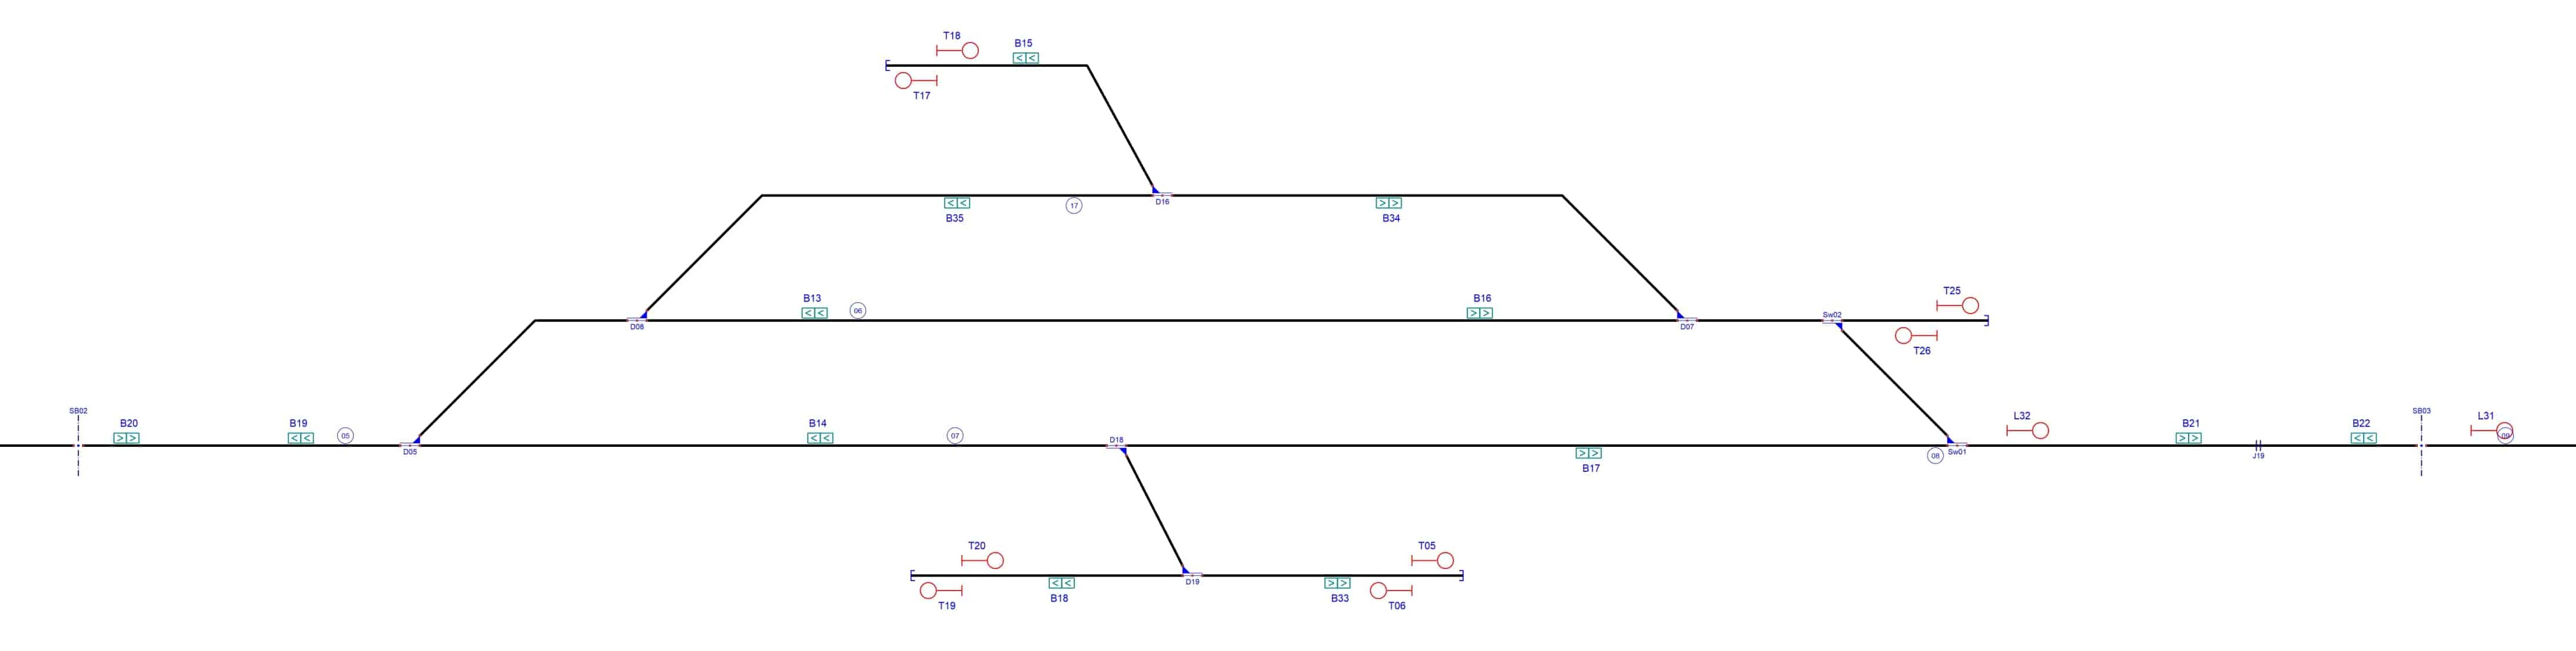
\includegraphics[width=1\textwidth]{resultados-obtenidos/ejemplo4/images/4_step1.png}
		\centering\caption{Señalamiento generado por el RNA para proteger el fin de vía.}
		\label{fig:EJ4_3}
	\end{figure}

	Los finales de vías absolutos son protegidos por las señales de parada T01, T03, T05, T07, T09, T11, T13, T15, T17, T19, T21, T23, T25 y T27; y las señales de partida son T02, T04, T06, T08, T10, T12, T14, T16, T18, T20, T22, T24, T26 y T28. A su vez, al no existir finales de vías relativos, el RNA no les asignó señales específicas.
	
	La Figura \ref{fig:EJ4_4} ilustra la generación de señales destinadas a proteger las junturas entre los rieles. Estas señales se obtuvieron al aplicar el Algoritmo \ref{alg:RJ}, tal como fue explicado en la Sección \ref{sec:sig_joint}. Las señales generadas son todas las señales entre J34 y J49, indicadas en color rojo. De no existir junturas que proteger, el RNA salteará este paso.

	\begin{figure}[H]
		\centering
		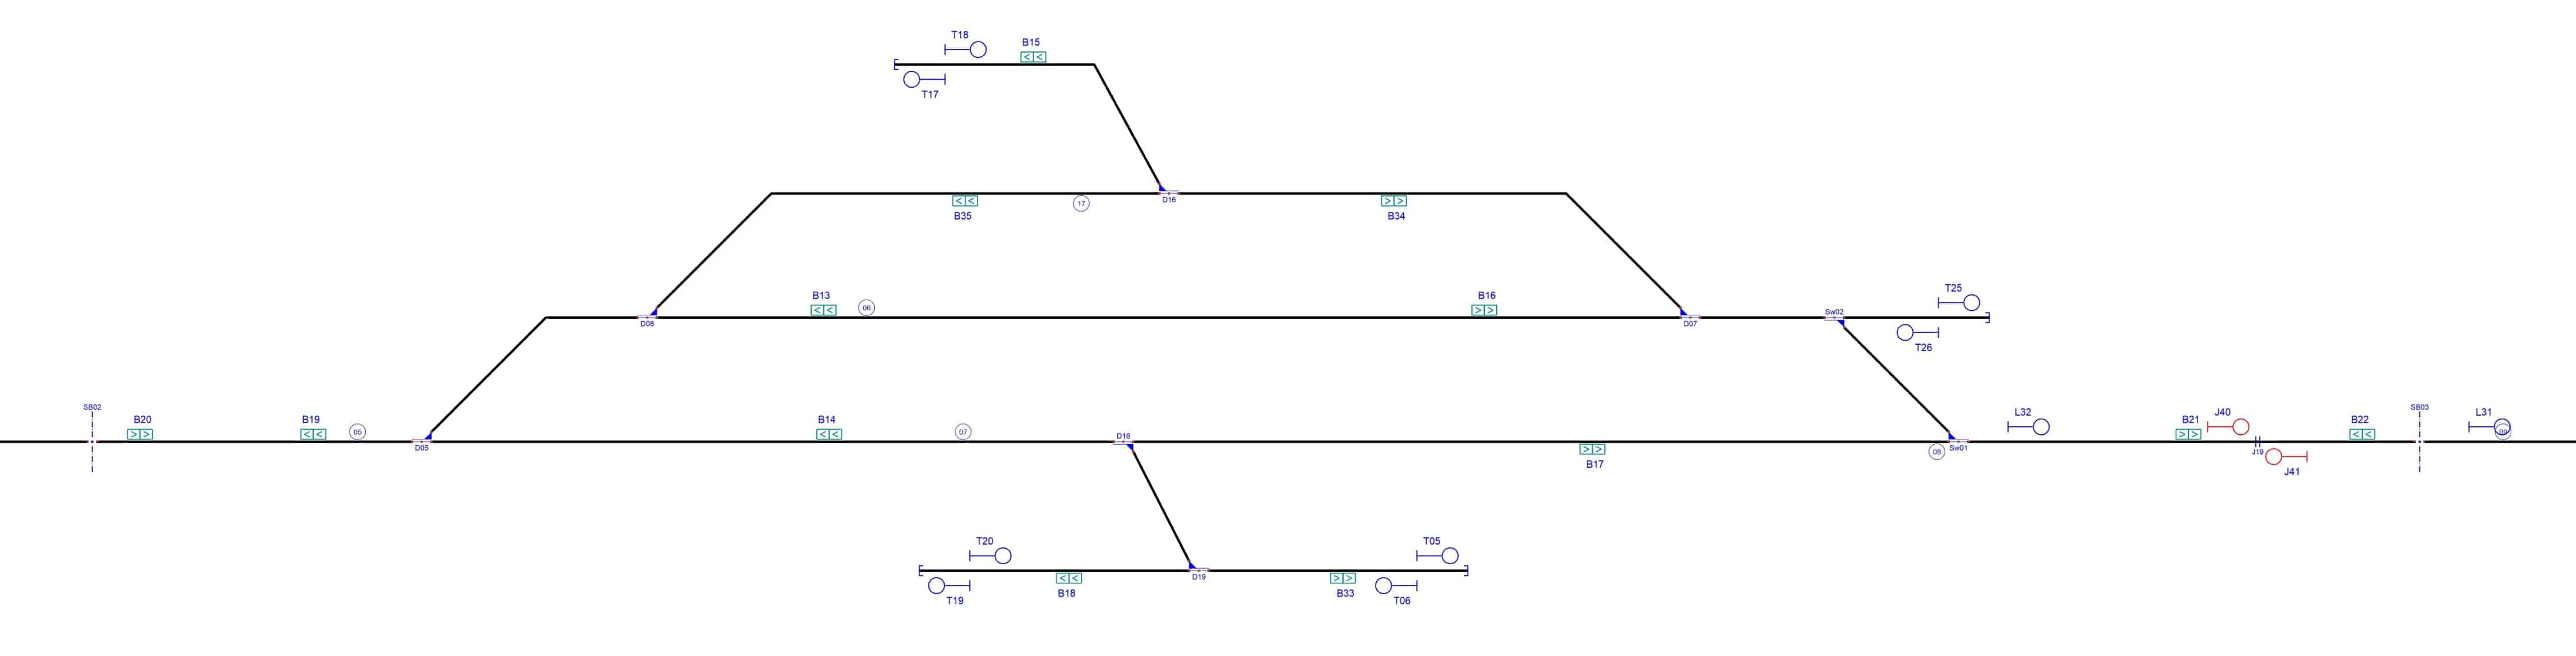
\includegraphics[width=1\textwidth]{resultados-obtenidos/ejemplo4/images/4_step2.png}
		\centering\caption{Señalamiento generado por el RNA para proteger las junturas.}
		\label{fig:EJ4_4}
	\end{figure}

	Al generar el señalamiento para proteger la infraestructura, tal como se explicó en la Sección \ref{sec:horizontal}, el Algoritmo \ref{alg:horizontal} simplificará las señales entre dos elementos ferroviarios si no existe espacio suficiente entre ellos. El señalamiento generado para proteger las plataformas y los cruces de vía, producto de aplicar el Algoritmo \ref{alg:PTF} y el Algoritmo \ref{alg:LC}, respectivamente, se ilustra en rojo en la Figura \ref{fig:EJ1_5}. No se asignaron señales para proteger las plataformas, al no existir en este ejemplo. Por otro lado, las señales que protegen los cruces de vía son las señales comprendidas entre X50 y X53.

	\begin{figure}[H]
		\centering
		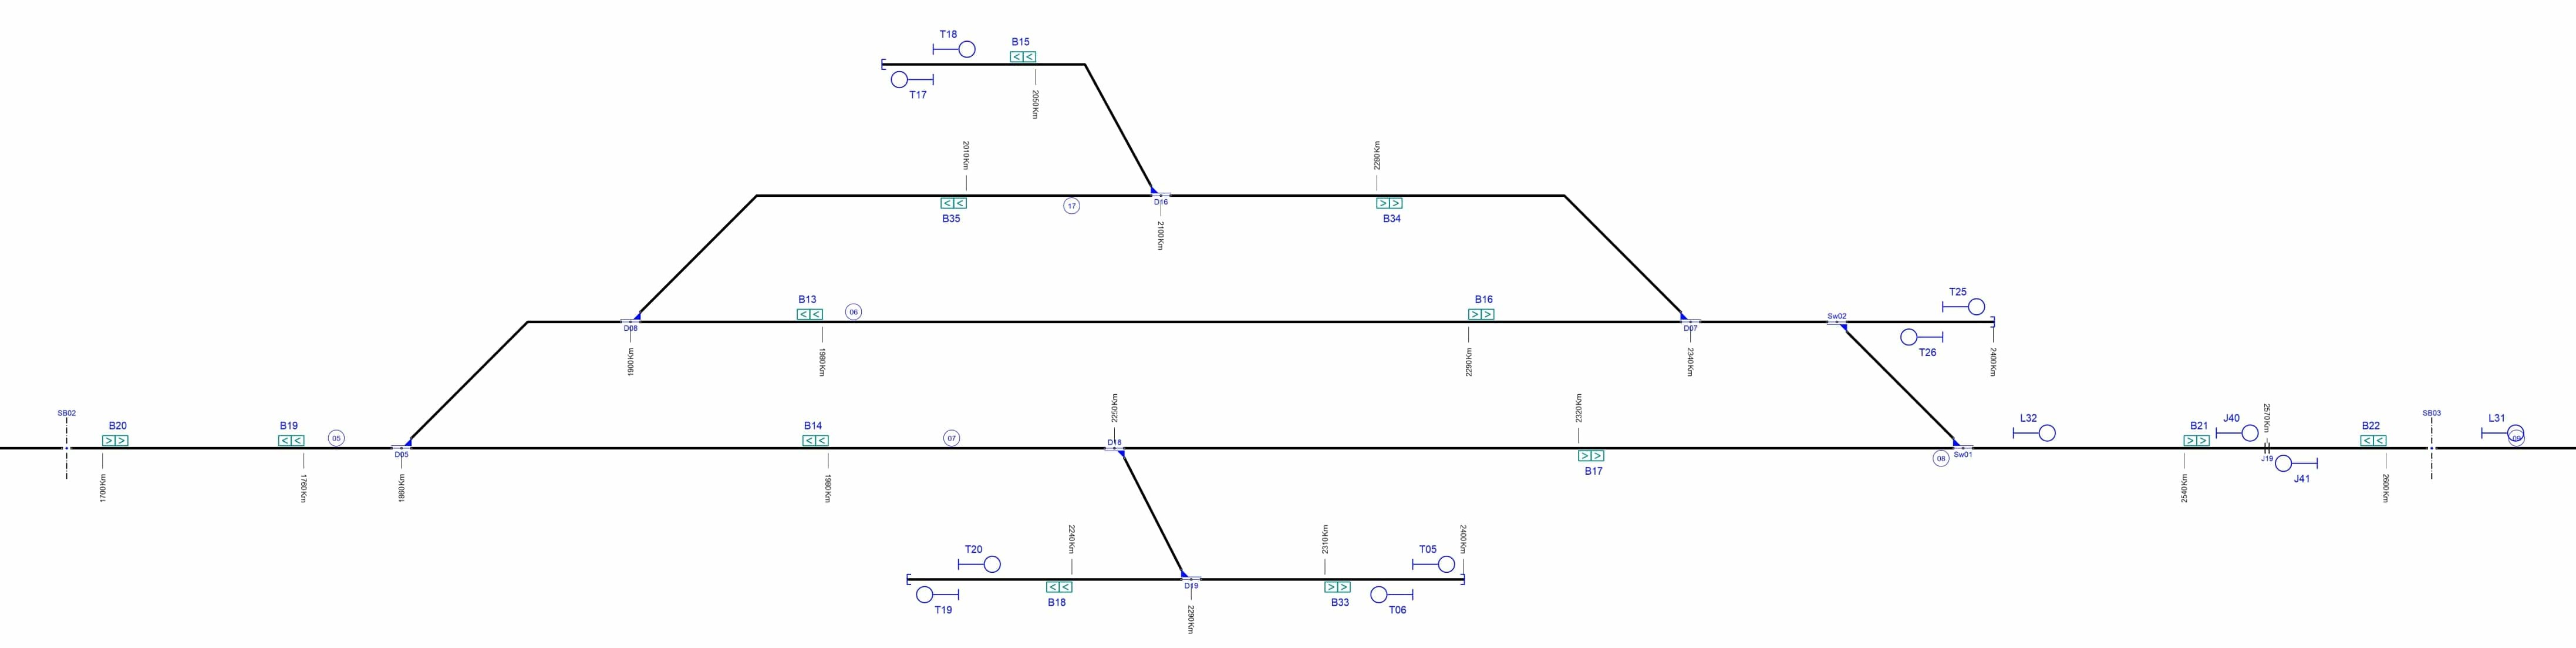
\includegraphics[width=1\textwidth]{resultados-obtenidos/ejemplo4/images/4_step3.png}
		\centering\caption{Señalamiento generado por el RNA para proteger plataformas y cruces de vía.}
		\label{fig:EJ4_5}
	\end{figure}

	Al aplicar el Algoritmo \ref{alg:SW} de generación de señalamiento para cambios de vías, tal como fue explicado en la Sección \label{sec:signal_switches}, el RNA generó 75 señales para proteger cada uno de los cambio de vías. Estas señales se encuentran resaltadas en rojo en la Figura \ref{fig:EJ4_6}.

	\begin{figure}[H]
		\centering
		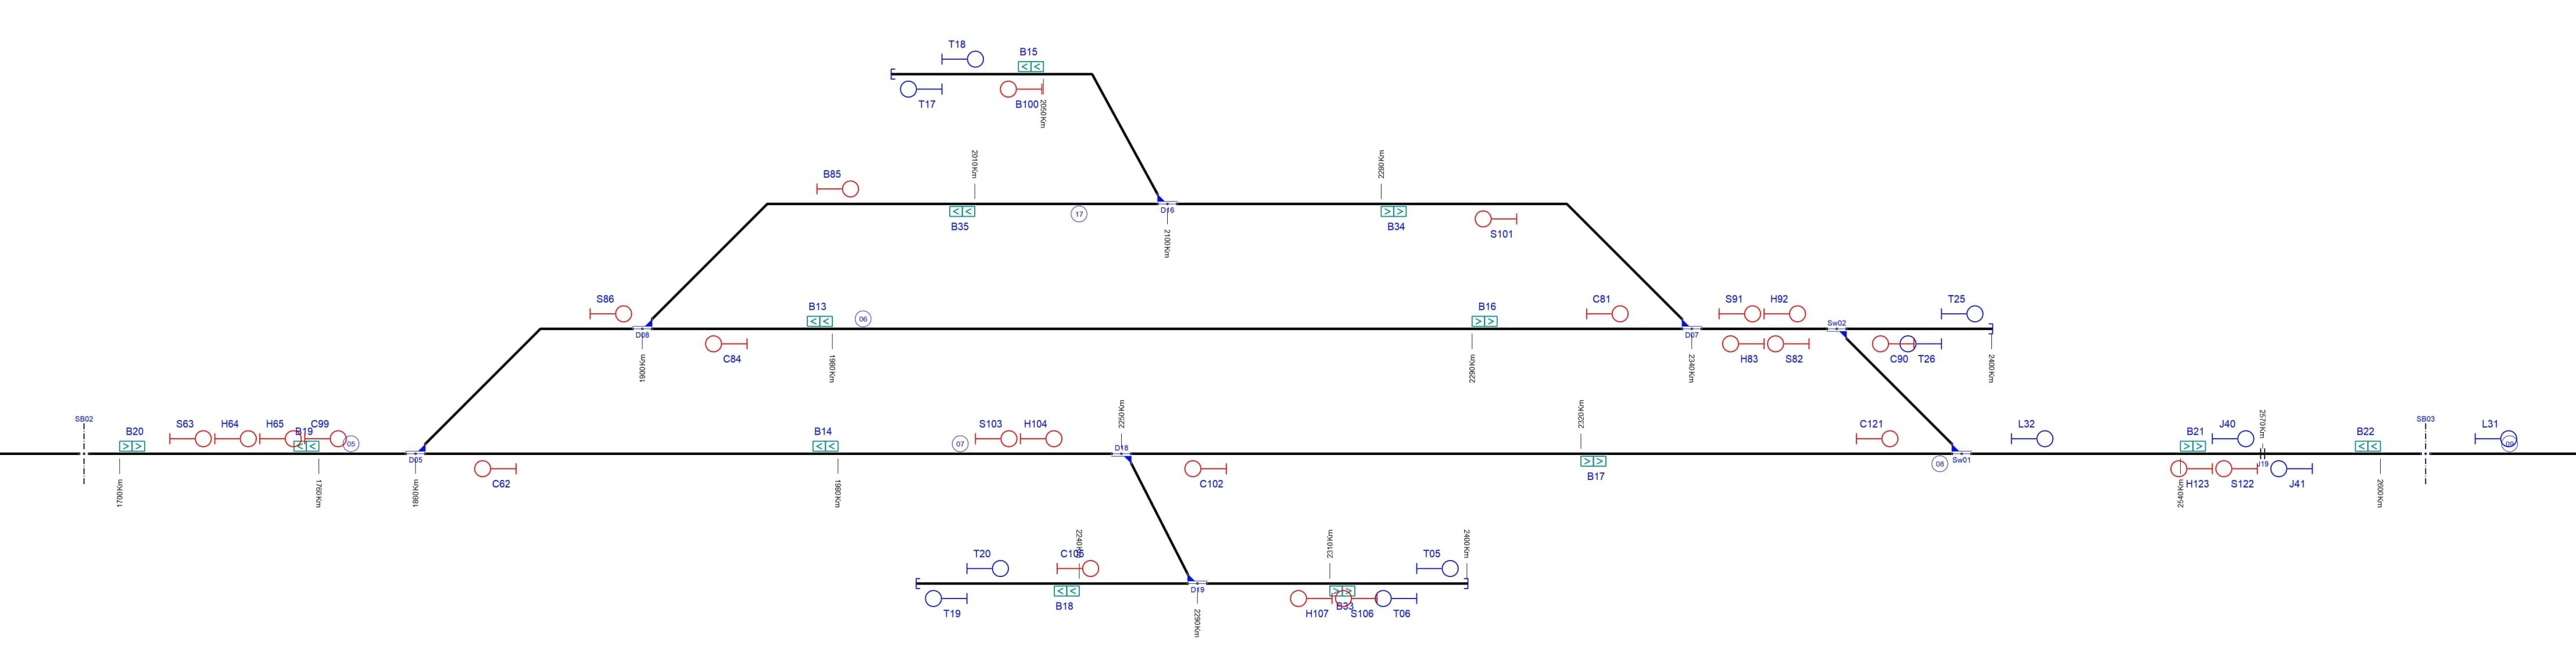
\includegraphics[width=1\textwidth]{resultados-obtenidos/ejemplo4/images/4_step4.png}
		\centering\caption{Señalamiento generado por el RNA para proteger los cambios de vías.}
		\label{fig:EJ4_6}
	\end{figure}

	Una vez obtenido todo el señalamiento, el RNA procede a simplificar las señales redundantes, repetidas o cuyas funciones o ubicaciones se superponen entre sí. El proceso de simplificación de señales fue explicado en la Sección \ref{sec:simplificacion}. El Algoritmo \ref{alg:vertical} de herencia vertical fue aplicado en las señales B entre los cambios de vías que comparan al menos una rama secundaria, desplazando las señales hasta convertirlas en las señales de herencia en las ramas principales. A continuación, se aplicó el Algoritmo \ref{alg:horizontal}, diseñado para agrupar objetos cercanos como un único objeto, generando el señalamiento acorde a los elementos contenidos en cada extremo del nuevo elemento contenedor.
		
	Finalmente, las señales son simplificadas aplicando el Algoritmo \ref{alg:reduction} de eliminación por prioridad de señales. El resultado de este proceso es detallado en el Código \ref{lst:EJ4_3}.

\begin{lstlisting}[language = {}, tabsize=4, basicstyle=\footnotesize\ttfamily, showspaces=false, showstringspaces=false, caption = Reducción de señalamiento por prioridad de señales, label = {lst:EJ4_3}]
	Reducing redundant signals
	removing sig97 for sig04
	removing sig98 for sig04
	removing sig106 for sig06
	removing sig107 for sig06
	removing sig115 for sig10
	removing sig116 for sig10
	removing sig96 for sig16
	removing sig100 for sig17
	removing sig105 for sig20
	removing sig114 for sig22
	removing sig118 for sig23
	removing sig90 for sig26
	removing sig124 for sig28
	removing sig32 for sig40
	removing sig33 for sig38
	removing sig34 for sig94
	removing sig70 for sig35
	removing sig127 for sig36
	removing sig93 for sig37
	removing sig39 for sig128
	removing sig41 for sig122
	removing sig42 for sig67
	removing sig44 for sig112
	removing sig66 for sig45
	removing sig108 for sig46
	removing sig111 for sig47
	removing sig49 for sig109
	removing sig50 for sig52
	removing sig51 for sig53
	removing sig54 for sig58
	removing sig55 for sig59
	removing sig56 for sig60
	removing sig57 for sig61
	removing sig99 for sig63
	removing sig64 for sig63
	removing sig65 for sig63
	removing sig117 for sig67
	removing sig68 for sig67
	removing sig69 for sig67
	removing sig72 for sig71
	removing sig73 for sig71
	removing sig80 for sig79
	removing sig83 for sig82
	removing sig92 for sig91
	removing sig95 for sig94
	removing sig104 for sig103
	removing sig110 for sig109
	removing sig113 for sig112
	removing sig120 for sig119
	removing sig123 for sig122
	removing sig126 for sig125
	removing sig129 for sig128
\end{lstlisting}

	El resultado de la simplificación del señalamiento se ilustra en la Figura \ref{fig:EJ4_7}.
	
	\begin{figure}[H]
		\centering
		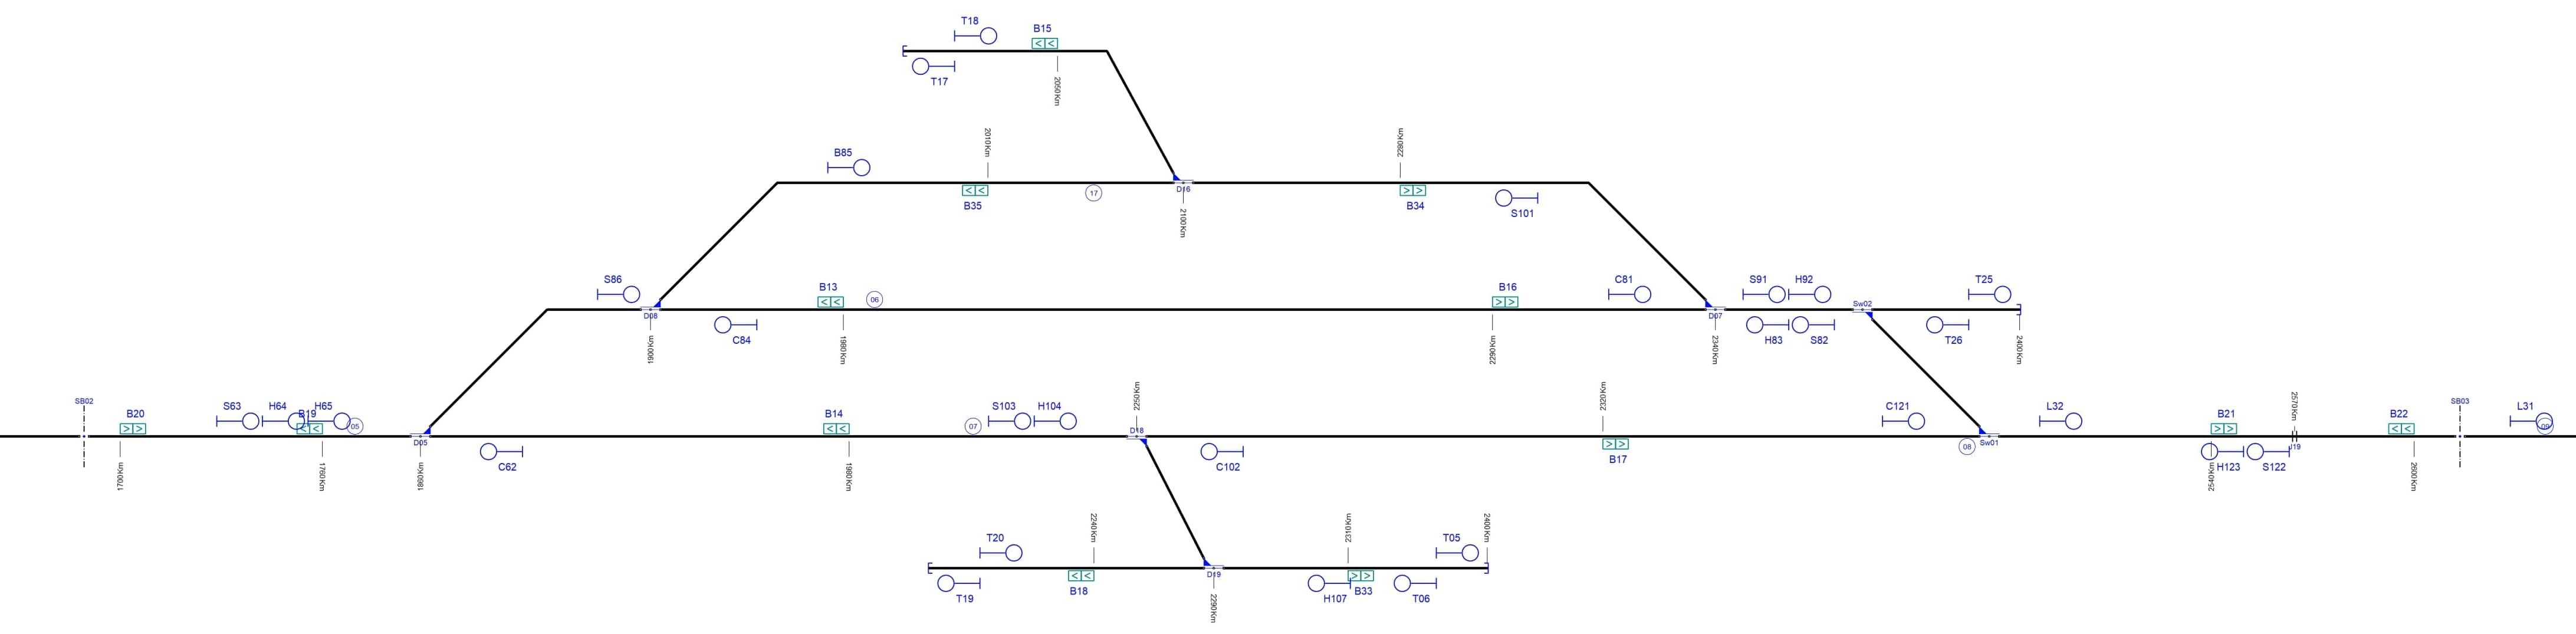
\includegraphics[width=1\textwidth]{resultados-obtenidos/ejemplo4/images/4_RNA.png}
		\centering\caption{Señalamiento generado y simplificado por el RNA.}
		\label{fig:EJ4_7}
	\end{figure}
	
	Además, toda la información del señalamiento generado es exportada por el RNA en el archivo Signalling.RNA (Código \ref{lst:EJ4_6}), que incluye información detallada de la posición, orientación, sentido, coordenada, nombre y tipo de señal.
	
	\begin{lstlisting}[language = {}, tabsize=4, basicstyle=\footnotesize\ttfamily, showspaces=false, showstringspaces=false, caption = Signalling.RNA, label = {lst:EJ4_6}]
T01 [T01] <<:
	From: ne991 | To: E16_left
	Type: Stop | Direction: normal | AtTrack: left 
	Position: [-2222, 0] | Coordinate: 0.0794
T02 [T02] >>:
	From: ne991 | To: ne991_right
	Type: Stop | Direction: reverse | AtTrack: right 
	Position: [-2222, 0] | Coordinate: 0.0794
T03 [T03] >>:
	From: ne377 | To: E305_right
	Type: Stop | Direction: reverse | AtTrack: right 
	Position: [250, 200] | Coordinate: 0.7737
T04 [T04] <<:
	From: ne377 | To: ne377_left
	Type: Stop | Direction: normal | AtTrack: left 
	Position: [250, 200] | Coordinate: 0.7737
T05 [T05] >>:
	From: ne421 | To: E418_right
	Type: Stop | Direction: reverse | AtTrack: right 
	Position: [6354, 259] | Coordinate: 0.8144
T06 [T06] <<:
	From: ne421 | To: ne421_left
	Type: Stop | Direction: normal | AtTrack: left 
	Position: [6354, 259] | Coordinate: 0.8144
T07 [T07] >>:
	From: ne450 | To: E478_right
	Type: Stop | Direction: reverse | AtTrack: right 
	Position: [14622, -250] | Coordinate: 0.7959
T08 [T08] <<:
	From: ne450 | To: ne450_left
	Type: Stop | Direction: normal | AtTrack: left 
	Position: [14622, -250] | Coordinate: 0.7959
T09 [T09] >>:
	From: ne465 | To: E462_right
	Type: Stop | Direction: reverse | AtTrack: right 
	Position: [13672, 259] | Coordinate: 0.8035
T10 [T10] <<:
	From: ne465 | To: ne465_left
	Type: Stop | Direction: normal | AtTrack: left 
	Position: [13672, 259] | Coordinate: 0.8035
T11 [T11] >>:
	From: ne102 | To: E109_right
	Type: Stop | Direction: normal | AtTrack: left 
	Position: [18072, 0] | Coordinate: 0.9600
T12 [T12] <<:
	From: ne102 | To: ne102_left
	Type: Stop | Direction: reverse | AtTrack: right 
	Position: [18072, 0] | Coordinate: 0.9600
T13 [T13] <<:
	From: ne104 | To: bus541_left
	Type: Stop | Direction: reverse | AtTrack: right 
	Position: [-409, -630] | Coordinate: 0.6065
T14 [T14] >>:
	From: ne104 | To: ne104_right
	Type: Stop | Direction: normal | AtTrack: left 
	Position: [-409, -630] | Coordinate: 0.6065
T15 [T15] <<:
	From: ne113 | To: E368_left
	Type: Stop | Direction: normal | AtTrack: left 
	Position: [-649, 200] | Coordinate: 0.1522
T16 [T16] >>:
	From: ne113 | To: ne113_right
	Type: Stop | Direction: reverse | AtTrack: right 
	Position: [-649, 200] | Coordinate: 0.1522
T17 [T17] <<:
	From: ne122 | To: E408_left
	Type: Stop | Direction: reverse | AtTrack: right 
	Position: [5404, -759] | Coordinate: 0.5713
T18 [T18] >>:
	From: ne122 | To: ne122_right
	Type: Stop | Direction: normal | AtTrack: left 
	Position: [5404, -759] | Coordinate: 0.5713
T19 [T19] <<:
	From: ne126 | To: E422_left
	Type: Stop | Direction: normal | AtTrack: left 
	Position: [5454, 259] | Coordinate: 0.1782
T20 [T20] >>:
	From: ne126 | To: ne126_right
	Type: Stop | Direction: reverse | AtTrack: right 
	Position: [5454, 259] | Coordinate: 0.1782
T21 [T21] <<:
	From: ne133 | To: E466_left
	Type: Stop | Direction: normal | AtTrack: left 
	Position: [12822, 259] | Coordinate: 0.1848
T22 [T22] >>:
	From: ne133 | To: ne133_right
	Type: Stop | Direction: reverse | AtTrack: right 
	Position: [12822, 259] | Coordinate: 0.1848
T23 [T23] <<:
	From: ne134 | To: bus570_left
	Type: Stop | Direction: reverse | AtTrack: right 
	Position: [12552, -810] | Coordinate: 0.6125
T24 [T24] >>:
	From: ne134 | To: ne134_right
	Type: Stop | Direction: normal | AtTrack: left 
	Position: [12552, -810] | Coordinate: 0.6125
T25 [T25] >>:
	From: ne993 | To: E412_right
	Type: Stop | Direction: normal | AtTrack: left 
	Position: [7404, -250] | Coordinate: 0.6774
T27 [T27] >>:
	From: ne995 | To: E313_right
	Type: Stop | Direction: normal | AtTrack: left 
	Position: [920, -250] | Coordinate: 0.6666
L29 [L29] >>:
	From: ne114 | To: sb540_left
	Type: Circulation | Direction: reverse | AtTrack: right 
	Position: [14582, 0] | Coordinate: 0.0841
L30 [L30] >>:
	From: ne98 | To: sb537_left
	Type: Circulation | Direction: normal | AtTrack: left 
	Position: [1673, 0] | Coordinate: 0.0473
L31 [L31] >>:
	From: ne100 | To: sb539_left
	Type: Circulation | Direction: normal | AtTrack: left 
	Position: [8472, 0] | Coordinate: 0.0424
J35 [J35] <<:
	From: ne290 | To: ne290_left
	Type: Circulation | Direction: reverse | AtTrack: right 
	Position: [-533.0, 0] | Coordinate: 0.6225
J36 [J36] >>:
	From: ne292 | To: ne292_right
	Type: Circulation | Direction: reverse | AtTrack: right 
	Position: [438.0, 0] | Coordinate: 0.6037
J37 [J37] <<:
	From: ne292 | To: ne292_left
	Type: Circulation | Direction: normal | AtTrack: left 
	Position: [638.0, 0] | Coordinate: 0.7897
J38 [J38] >>:
	From: ne996 | To: ne996_right
	Type: Circulation | Direction: normal | AtTrack: left 
	Position: [994.0, 0] | Coordinate: 0.1833
J40 [J40] >>:
	From: ne992 | To: ne992_right
	Type: Circulation | Direction: normal | AtTrack: left 
	Position: [7946.0, 0] | Coordinate: 0.5409
J43 [J43] <<:
	From: ne101 | To: ne101_left
	Type: Circulation | Direction: reverse | AtTrack: right 
	Position: [11014.0, 0] | Coordinate: 0.5445
J45 [J45] <<:
	From: ne912 | To: ne912_left
	Type: Circulation | Direction: reverse | AtTrack: right 
	Position: [11967.0, 0] | Coordinate: 0.3839
J46 [J46] >>:
	From: ne132 | To: ne132_right
	Type: Circulation | Direction: normal | AtTrack: left 
	Position: [14209.0, 0] | Coordinate: 0.8008
J47 [J47] <<:
	From: ne132 | To: ne132_left
	Type: Circulation | Direction: reverse | AtTrack: right 
	Position: [14409.0, 0] | Coordinate: 0.9467
J48 [J48] >>:
	From: ne114 | To: ne114_right
	Type: Circulation | Direction: reverse | AtTrack: right 
	Position: [15194.0, 0] | Coordinate: 0.5993
X50 [X50] >>:
	From: ne98 | To: ne98_right
	Type: Circulation | Direction: normal | AtTrack: left 
	Position: [2219, 0] | Coordinate: 0.3055
X51 [X51] <<:
	From: ne98 | To: ne98_left
	Type: Circulation | Direction: reverse | AtTrack: right 
	Position: [2619, 0] | Coordinate: 0.4947
X52 [X52] >>:
	From: ne100 | To: ne100_right
	Type: Circulation | Direction: normal | AtTrack: left 
	Position: [9927, 0] | Coordinate: 0.6602
X53 [X53] <<:
	From: ne100 | To: ne100_left
	Type: Circulation | Direction: reverse | AtTrack: right 
	Position: [10327, 0] | Coordinate: 0.8301
C54 [C54] <<:
	From: ne63 | To: ne63_left
	Type: Circulation | Direction: reverse | AtTrack: right 
	Position: [4551.9, 0] | Coordinate: 0.1428
S55 [S55] >>:
	From: ne99 | To: ne99_right
	Type: Circulation | Direction: normal | AtTrack: left 
	Position: [4129.0, 0] | Coordinate: 0.6666
S59 [S59] >>:
	From: ne101 | To: ne101_right
	Type: Circulation | Direction: normal | AtTrack: left 
	Position: [11014.0, 0] | Coordinate: 0.5445
S64 [S64] >>:
	From: ne991 | To: ne991_right
	Type: Circulation | Direction: reverse | AtTrack: right 
	Position: [-1273.7, 0] | Coordinate: 0.8333
C67 [C67] <<:
	From: ne295 | To: ne295_left
	Type: Circulation | Direction: reverse | AtTrack: right 
	Position: [-501.4, -250] | Coordinate: 0.2
B68 [B68] >>:
	From: ne110 | To: ne110_left
	Type: Manouver | Direction: reverse | AtTrack: right 
	Position: [-533.0, -450] | Coordinate: 0.4327
S69 [S69] >>:
	From: ne288 | To: ne288_right
	Type: Circulation | Direction: normal | AtTrack: left 
	Position: [-828.0, -250] | Coordinate: 0.8155
C70 [C70] >>:
	From: ne295 | To: ne295_right
	Type: Circulation | Direction: normal | AtTrack: left 
	Position: [217.4, -250] | Coordinate: 0.7999
B71 [B71] <<:
	From: ne384 | To: ne384_right
	Type: Manouver | Direction: normal | AtTrack: left 
	Position: [250.0, -450] | Coordinate: 0.8531
S72 [S72] <<:
	From: ne297 | To: ne297_left
	Type: Circulation | Direction: reverse | AtTrack: right 
	Position: [588.5, -250] | Coordinate: 0.5
C74 [C74] >>:
	From: ne404 | To: ne404_right
	Type: Circulation | Direction: normal | AtTrack: left 
	Position: [6694.0, -250] | Coordinate: 0.9
S75 [S75] <<:
	From: ne400 | To: ne400_left
	Type: Circulation | Direction: reverse | AtTrack: right 
	Position: [7049.0, -250] | Coordinate: 0.5
C77 [C77] <<:
	From: ne404 | To: ne404_left
	Type: Circulation | Direction: reverse | AtTrack: right 
	Position: [5014.0, -250] | Coordinate: 0.1
B78 [B78] >>:
	From: ne123 | To: ne123_left
	Type: Manouver | Direction: reverse | AtTrack: right 
	Position: [5154.0, -500] | Coordinate: 0.3928
S79 [S79] >>:
	From: ne61 | To: ne61_right
	Type: Circulation | Direction: normal | AtTrack: left 
	Position: [4700.0, -250] | Coordinate: 0.8134
C80 [C80] <<:
	From: ne130 | To: ne130_left
	Type: Circulation | Direction: normal | AtTrack: left 
	Position: [12022.8, -250] | Coordinate: 0.0833
B81 [B81] >>:
	From: ne135 | To: ne135_left
	Type: Manouver | Direction: reverse | AtTrack: right 
	Position: [12172.0, -500] | Coordinate: 0.3479
S82 [S82] >>:
	From: ne910 | To: ne910_right
	Type: Circulation | Direction: normal | AtTrack: left 
	Position: [11604.0, -250] | Coordinate: 0.6753
C83 [C83] <<:
	From: ne993 | To: ne993_left
	Type: Circulation | Direction: reverse | AtTrack: right 
	Position: [7349.0, -250] | Coordinate: 0.5
S84 [S84] >>:
	From: ne400 | To: ne400_right
	Type: Circulation | Direction: normal | AtTrack: left 
	Position: [7049.0, -250] | Coordinate: 0.5
S87 [S87] >>:
	From: ne290 | To: ne290_right
	Type: Circulation | Direction: normal | AtTrack: left 
	Position: [-533.0, 0] | Coordinate: 0.6225
S94 [S94] <<:
	From: ne407 | To: ne407_left
	Type: Circulation | Direction: normal | AtTrack: left 
	Position: [6554.0, -500] | Coordinate: 0.9132
C95 [C95] <<:
	From: ne65 | To: ne65_left
	Type: Circulation | Direction: normal | AtTrack: left 
	Position: [5973.1, 0] | Coordinate: 0.1249
S96 [S96] >>:
	From: ne63 | To: ne63_right
	Type: Circulation | Direction: normal | AtTrack: left 
	Position: [5561.1, 0] | Coordinate: 0.8571
S102 [S102] <<:
	From: ne114 | To: ne114_left
	Type: Circulation | Direction: normal | AtTrack: left 
	Position: [15194.0, 0] | Coordinate: 0.5993
S105 [S105] >>:
	From: ne127 | To: ne127_right
	Type: Circulation | Direction: reverse | AtTrack: right 
	Position: [13882.0, -500] | Coordinate: 0.9238
S108 [S108] >>:
	From: ne130 | To: ne130_right
	Type: Circulation | Direction: reverse | AtTrack: right 
	Position: [14031.2, -250] | Coordinate: 0.9166
S111 [S111] >>:
	From: ne912 | To: ne912_right
	Type: Circulation | Direction: normal | AtTrack: left 
	Position: [11967.0, 0] | Coordinate: 0.3839
S118 [S118] <<:
	From: ne127 | To: ne127_left
	Type: Circulation | Direction: normal | AtTrack: left 
	Position: [13882.0, -500] | Coordinate: 0.9238
C120 [C120] >>:
	From: ne65 | To: ne65_right
	Type: Circulation | Direction: reverse | AtTrack: right 
	Position: [7233.9, 0] | Coordinate: 0.8750
S121 [S121] <<:
	From: ne992 | To: ne992_left
	Type: Circulation | Direction: reverse | AtTrack: right 
	Position: [7946.0, 0] | Coordinate: 0.5409
C123 [C123] <<:
	From: ne995 | To: ne995_left
	Type: Circulation | Direction: reverse | AtTrack: right 
	Position: [870.0, -250] | Coordinate: 0.5
S124 [S124] >>:
	From: ne297 | To: ne297_right
	Type: Circulation | Direction: normal | AtTrack: left 
	Position: [588.5, -250] | Coordinate: 0.5
S127 [S127] <<:
	From: ne996 | To: ne996_left
	Type: Circulation | Direction: reverse | AtTrack: right 
	Position: [994.0, 0] | Coordinate: 0.1833
	\end{lstlisting}	
	
	Al finalizar la generación del señalamiento, el RNA ejecuta el Algoritmo \ref{alg:routes}, explicado en la Sección \ref{sec:rutas}, para detectar todas las posibles rutas admitidas por la red para crear la tabla de enclavamientos. La cuál puede ser visualizada en el archivo Routes.RNA (Código \ref{lst:EJ4_7}). La misma detalla las señales de inicio y final, los \textit{netElements} abarcados por la ruta y cualquier infraestructura involucrada, incluyendo el estado que deben tener para que la ruta sea activada.
	
	\begin{lstlisting}[language = {}, tabsize=4, basicstyle=\footnotesize\ttfamily, showspaces=false, showstringspaces=false, caption = Routes.RNA, label = {lst:EJ4_7}]
route_1 [T02 >> S64]:
	Path: ['ne991']
route_2 [T04 << J35]:
	Path: ['ne377', 'ne111', 'ne290']
	Switches: ['D14_R', 'D15_R']
route_3 [T04 << T15]:
	Path: ['ne377', 'ne113']
	Switches: ['D15_N']
route_4 [T06 << C54]:
	Path: ['ne421', 'ne124', 'ne63']
	Switches: ['D18_R', 'D19_R']
route_5 [T06 << T19]:
	Path: ['ne421', 'ne126']
	Switches: ['D19_N']
route_6 [T08 << S118]:
	Path: ['ne450', 'ne127']
	Switches: ['D12_RN']
route_7 [T08 << C80]:
	Path: ['ne450', 'ne130']
	Switches: ['D12_NN']
route_8 [T10 << J45]:
	Path: ['ne465', 'ne131', 'ne912']
	Switches: ['D20_R', 'D21_R']
route_9 [T10 << T21]:
	Path: ['ne465', 'ne133']
	Switches: ['D21_N']
route_10 [T12 << S102]:
	Path: ['ne102', 'ne114']
route_11 [T14 >> S124]:
	Path: ['ne104', 'ne384', 'ne297']
	Switches: ['D04_R']
route_12 [T16 >> T03]:
	Path: ['ne113', 'ne377']
	Switches: ['D15_N']
route_13 [T18 >> S84]:
	Path: ['ne122', 'ne407', 'ne400']
	Switches: ['D07_R', 'D16_R']
route_14 [T20 >> T05]:
	Path: ['ne126', 'ne421']
	Switches: ['D19_N']
route_15 [T22 >> T09]:
	Path: ['ne133', 'ne465']
	Switches: ['D21_N']
route_16 [T24 >> S105]:
	Path: ['ne134', 'ne127']
	Switches: ['D24_R']
route_17 [L29 >> J48]:
	Path: ['ne114']
route_18 [L30 >> X50]:
	Path: ['ne98']
route_19 [L31 >> X52]:
	Path: ['ne100']
route_20 [J35 << T01]:
	Path: ['ne290', 'ne991']
	Switches: ['D01_N']
route_21 [J36 >> J38]:
	Path: ['ne292', 'ne996']
	Switches: ['Sw04_N']
route_22 [J37 << J35]:
	Path: ['ne292', 'ne290']
	Switches: ['D14_N']
route_23 [J38 >> L30]:
	Path: ['ne996', 'ne98']
route_24 [J40 >> L31]:
	Path: ['ne992', 'ne100']
route_25 [J43 << X53]:
	Path: ['ne101', 'ne100']
route_26 [J45 << J43]:
	Path: ['ne912', 'ne101']
	Switches: ['D09_N']
route_27 [J46 >> L29]:
	Path: ['ne132', 'ne114']
	Switches: ['D23_N']
route_28 [J47 << J45]:
	Path: ['ne132', 'ne912']
	Switches: ['D20_N']
route_29 [J48 >> T11]:
	Path: ['ne114', 'ne102']
route_30 [X50 >> S55]:
	Path: ['ne98', 'ne99']
	LevelCrossings: ['Lc01']
route_31 [X51 << S127]:
	Path: ['ne98', 'ne996']
	LevelCrossings: ['Lc01']
route_32 [X52 >> S59]:
	Path: ['ne100', 'ne101']
	LevelCrossings: ['Lc04']
route_33 [X53 << S121]:
	Path: ['ne100', 'ne992']
	LevelCrossings: ['Lc04']
route_34 [C54 << X51]:
	Path: ['ne63', 'ne99', 'ne98']
	Switches: ['D05_N']
route_35 [S55 >> S79]:
	Path: ['ne99', 'ne61']
	Switches: ['D05_R']
route_36 [S55 >> S96]:
	Path: ['ne99', 'ne63']
	Switches: ['D05_N']
route_37 [S59 >> S111]:
	Path: ['ne101', 'ne912']
	Switches: ['D09_N']
route_38 [S59 >> S82]:
	Path: ['ne101', 'ne910']
	Switches: ['D09_R']
route_39 [S64 >> S69]:
	Path: ['ne991', 'ne288']
	Switches: ['D01_R']
route_40 [S64 >> S87]:
	Path: ['ne991', 'ne290']
	Switches: ['D01_N']
route_41 [C67 << T01]:
	Path: ['ne295', 'ne288', 'ne991']
	Switches: ['D01_R', 'D03_N']
route_42 [B68 >> S124]:
	Path: ['ne110', 'ne384', 'ne297']
	Switches: ['D04_R']
route_43 [S69 >> C70]:
	Path: ['ne288', 'ne295']
	Switches: ['D03_N']
route_44 [S69 >> B68]:
	Path: ['ne288', 'ne110']
	Switches: ['D03_R']
route_45 [C70 >> S124]:
	Path: ['ne295', 'ne297']
	Switches: ['D04_N']
route_46 [B71 << T13]:
	Path: ['ne384', 'ne104']
route_47 [B71 << T01]:
	Path: ['ne384', 'ne110', 'ne288', 'ne991']
	Switches: ['D01_R', 'D03_R']
route_48 [S72 << C67]:
	Path: ['ne297', 'ne295']
	Switches: ['D04_N']
route_49 [S72 << B71]:
	Path: ['ne297', 'ne384']
	Switches: ['D04_R']
route_50 [C74 >> S84]:
	Path: ['ne404', 'ne400']
	Switches: ['D07_N']
route_51 [S75 << C77]:
	Path: ['ne400', 'ne404']
	Switches: ['D07_N']
route_52 [S75 << S94]:
	Path: ['ne400', 'ne407']
	Switches: ['D07_R']
route_53 [C77 << X51]:
	Path: ['ne404', 'ne61', 'ne99', 'ne98']
	Switches: ['D05_R', 'D08_N']
route_54 [B78 >> S84]:
	Path: ['ne123', 'ne407', 'ne400']
	Switches: ['D07_R', 'D16_N']
route_55 [S79 >> C74]:
	Path: ['ne61', 'ne404']
	Switches: ['D08_N']
route_56 [S79 >> B78]:
	Path: ['ne61', 'ne123']
	Switches: ['D08_R']
route_57 [C80 << J43]:
	Path: ['ne130', 'ne910', 'ne101']
	Switches: ['D09_R', 'D10_N']
route_58 [B81 >> S105]:
	Path: ['ne135', 'ne127']
	Switches: ['D24_N']
route_59 [S82 >> S108]:
	Path: ['ne910', 'ne130']
	Switches: ['D10_N']
route_60 [S82 >> B81]:
	Path: ['ne910', 'ne135']
	Switches: ['D10_R']
route_61 [C83 << S75]:
	Path: ['ne993', 'ne400']
	Switches: ['Sw02_N']
route_62 [S84 >> T25]:
	Path: ['ne400', 'ne993']
	Switches: ['Sw02_N']
route_63 [S84 >> J40]:
	Path: ['ne400', 'ne994', 'ne992']
	Switches: ['Sw02_R', 'Sw01_R']
route_64 [S87 >> J36]:
	Path: ['ne290', 'ne292']
	Switches: ['D14_N']
route_65 [S87 >> T03]:
	Path: ['ne290', 'ne111', 'ne377']
	Switches: ['D14_R', 'D15_R']
route_66 [S94 << T17]:
	Path: ['ne407', 'ne122']
	Switches: ['D16_R']
route_67 [S94 << X51]:
	Path: ['ne407', 'ne123', 'ne61', 'ne99', 'ne98']
	Switches: ['D05_R', 'D08_R', 'D16_N']
route_68 [C95 << C54]:
	Path: ['ne65', 'ne63']
	Switches: ['D18_N']
route_69 [S96 >> C120]:
	Path: ['ne63', 'ne65']
	Switches: ['D18_N']
route_70 [S96 >> T05]:
	Path: ['ne63', 'ne124', 'ne421']
	Switches: ['D18_R', 'D19_R']
route_71 [S102 << J47]:
	Path: ['ne114', 'ne132']
	Switches: ['D23_N']
route_72 [S102 << S118]:
	Path: ['ne114', 'ne129', 'ne127']
	Switches: ['D23_R', 'D12_RR']
route_73 [S102 << C80]:
	Path: ['ne114', 'ne129', 'ne130']
	Switches: ['D23_R', 'D12_NR']
route_74 [S105 >> L29]:
	Path: ['ne127', 'ne129', 'ne114']
	Switches: ['D23_R', 'D12_RR']
route_75 [S105 >> T07]:
	Path: ['ne127', 'ne450']
	Switches: ['D12_RN']
route_76 [S108 >> L29]:
	Path: ['ne130', 'ne129', 'ne114']
	Switches: ['D23_R', 'D12_NR']
route_77 [S108 >> T07]:
	Path: ['ne130', 'ne450']
	Switches: ['D12_NN']
route_78 [S111 >> T09]:
	Path: ['ne912', 'ne131', 'ne465']
	Switches: ['D20_R', 'D21_R']
route_79 [S111 >> J46]:
	Path: ['ne912', 'ne132']
	Switches: ['D20_N']
route_80 [S118 << J43]:
	Path: ['ne127', 'ne135', 'ne910', 'ne101']
	Switches: ['D09_R', 'D10_R', 'D24_N']
route_81 [S118 << T23]:
	Path: ['ne127', 'ne134']
	Switches: ['D24_R']
route_82 [C120 >> J40]:
	Path: ['ne65', 'ne992']
	Switches: ['Sw01_N']
route_83 [S121 << C95]:
	Path: ['ne992', 'ne65']
	Switches: ['Sw01_N']
route_84 [S121 << S75]:
	Path: ['ne992', 'ne994', 'ne400']
	Switches: ['Sw02_R', 'Sw01_R']
route_85 [C123 << S72]:
	Path: ['ne995', 'ne297']
	Switches: ['Sw03_N']
route_86 [S124 >> T27]:
	Path: ['ne297', 'ne995']
	Switches: ['Sw03_N']
route_87 [S124 >> J38]:
	Path: ['ne297', 'ne997', 'ne996']
	Switches: ['Sw03_R', 'Sw04_R']
route_88 [S127 << J37]:
	Path: ['ne996', 'ne292']
	Switches: ['Sw04_N']
route_89 [S127 << S72]:
	Path: ['ne996', 'ne997', 'ne297']
	Switches: ['Sw03_R', 'Sw04_R']
	\end{lstlisting}
    \section{Señalamiento generado por el RNA}

    El RNA también exporta la misma información mostrada en el Código \ref{lst:EJ4_8} en una hoja de cálculo, similar a la que se visualiza en las Tablas \ref{Tab:tabla_generated_4_1}, \ref{Tab:tabla_generated_4_2}, \ref{Tab:tabla_generated_4_3}, \ref{Tab:tabla_generated_4_4}, \ref{Tab:tabla_generated_4_5} y \ref{Tab:tabla_generated_4_6}.

    \begin{table}[H]
        {
        \caption{Tabla de enclavamiento del ejemplo 4 generada por el RNA (Rutas 1 a 15).}
        \label{Tab:tabla_generated_4_1}
        \centering
        \resizebox{1\textwidth}{!}{
            \begin{tabular}{ c c c c c c c }
                \hline	
                    Ruta & Inicio & Final & Cambio & Plataforma & Cruce & netElement \\	
                \hline
                    R$_{01}$ & T$_{02}$ & S$_{71}$ &  &  &  & ne$_{991}$-ne$_{991}$\\
                    R$_{02}$ & T$_{04}$ & J$_{35}$ & D$_{14}^{R}$-D$_{15}^{R}$ &  &  & ne$_{377}$-ne$_{290}$\\
                    R$_{03}$ & T$_{04}$ & T$_{15}$ & D$_{15}^{N}$ &  &  & ne$_{377}$-ne$_{113}$\\
                    R$_{04}$ & T$_{06}$ & C$_{62}$ & D$_{18}^{R}$-D$_{19}^{R}$ &  &  & ne$_{421}$-ne$_{63}$\\
                    R$_{05}$ & T$_{06}$ & T$_{19}$ & D$_{19}^{N}$ &  &  & ne$_{421}$-ne$_{126}$\\
                    R$_{06}$ & T$_{08}$ & S$_{119}$ &  &  &  & ne$_{450}$-ne$_{127}$\\
                    R$_{07}$ & T$_{08}$ & C$_{87}$ &  &  &  & ne$_{450}$-ne$_{130}$\\
                    R$_{08}$ & T$_{10}$ & J$_{45}$ & D$_{20}^{R}$-D$_{21}^{R}$ &  &  & ne$_{465}$-ne$_{912}$\\
                    R$_{09}$ & T$_{10}$ & T$_{21}$ & D$_{21}^{N}$ &  &  & ne$_{465}$-ne$_{133}$\\
                    R$_{10}$ & T$_{12}$ & S$_{109}$ &  &  &  & ne$_{102}$-ne$_{114}$\\
                    R$_{11}$ & T$_{14}$ & S$_{125}$ & D$_{04}^{R}$ &  &  & ne$_{104}$-ne$_{297}$\\
                    R$_{12}$ & T$_{16}$ & T$_{03}$ & D$_{15}^{N}$ &  &  & ne$_{113}$-ne$_{377}$\\
                    R$_{13}$ & T$_{18}$ & S$_{91}$ & D$_{07}^{R}$-D$_{16}^{R}$ &  &  & ne$_{122}$-ne$_{400}$\\
                    R$_{14}$ & T$_{20}$ & T$_{05}$ & D$_{19}^{N}$ &  &  & ne$_{126}$-ne$_{421}$\\
                    R$_{15}$ & T$_{22}$ & T$_{09}$ & D$_{21}^{N}$ &  &  & ne$_{133}$-ne$_{465}$\\
                \hline
            \end{tabular}
        }
     }
    \end{table}

	%\lipsum[1]
	
    \begin{table}[H]
        {
        \caption{Tabla de enclavamiento del ejemplo 4 generada por el RNA (Rutas 16 a 30).}
        \label{Tab:tabla_generated_4_2}
        \centering
        \resizebox{1\textwidth}{!}{
            \begin{tabular}{ c c c c c c c }
                \hline	
                    Ruta & Inicio & Final & Cambio & Plataforma & Cruce & netElement \\	
                \hline
                    R$_{16}$ & T$_{24}$ & S$_{105}$ & D$_{24}^{R}$ &  &  & ne$_{134}$-ne$_{127}$\\
                    R$_{17}$ & L$_{29}$ & J$_{48}$ &  &  &  & ne$_{114}$-ne$_{114}$\\
                    R$_{18}$ & S$_{30}$ & X$_{50}$ &  &  &  & ne$_{98}$-ne$_{98}$\\
                    R$_{19}$ & L$_{31}$ & X$_{52}$ &  &  &  & ne$_{100}$-ne$_{100}$\\
                    R$_{20}$ & J$_{35}$ & T$_{01}$ & D$_{01}^{N}$ &  &  & ne$_{290}$-ne$_{991}$\\
                    R$_{21}$ & J$_{36}$ & J$_{38}$ & Sw$_{04}^{N}$ &  &  & ne$_{292}$-ne$_{996}$\\
                    R$_{22}$ & J$_{37}$ & J$_{35}$ & D$_{14}^{N}$ &  &  & ne$_{292}$-ne$_{290}$\\
                    R$_{23}$ & J$_{38}$ & S$_{30}$ &  &  &  & ne$_{996}$-ne$_{98}$\\
                    R$_{24}$ & J$_{40}$ & L$_{31}$ &  &  &  & ne$_{992}$-ne$_{100}$\\
                    R$_{25}$ & J$_{43}$ & X$_{53}$ &  &  &  & ne$_{101}$-ne$_{100}$\\
                    R$_{26}$ & J$_{45}$ & J$_{43}$ & D$_{09}^{N}$ &  &  & ne$_{912}$-ne$_{101}$\\
                    R$_{27}$ & J$_{46}$ & L$_{29}$ & D$_{23}^{N}$ &  &  & ne$_{132}$-ne$_{114}$\\
                    R$_{28}$ & J$_{47}$ & J$_{45}$ & D$_{20}^{N}$ &  &  & ne$_{132}$-ne$_{912}$\\
                    R$_{29}$ & J$_{48}$ & T$_{11}$ &  &  &  & ne$_{114}$-ne$_{102}$\\
                    R$_{30}$ & X$_{50}$ & S$_{55}$ &  &  & Lc$_{01}$ & ne$_{98}$-ne$_{99}$\\
                \hline
            \end{tabular}
        }
     }
    \end{table}

	%\lipsum[1]
	
    \begin{table}[H]
        {
        \caption{Tabla de enclavamiento del ejemplo 4 generada por el RNA (Rutas 31 a 45).}
        \label{Tab:tabla_generated_4_3}
        \centering
        \resizebox{1\textwidth}{!}{
            \begin{tabular}{ c c c c c c c }
                \hline	
                    Ruta & Inicio & Final & Cambio & Plataforma & Cruce & netElement \\	
                \hline
                    R$_{31}$ & X$_{51}$ & S$_{127}$ &  &  & Lc$_{01}$ & ne$_{98}$-ne$_{996}$\\
                    R$_{32}$ & X$_{52}$ & S$_{59}$ &  &  & Lc$_{04}$ & ne$_{100}$-ne$_{101}$\\
                    R$_{33}$ & X$_{53}$ & S$_{121}$ &  &  & Lc$_{04}$ & ne$_{100}$-ne$_{992}$\\
                    R$_{34}$ & C$_{54}$ & X$_{51}$ & D$_{05}^{N}$ & & & ne$_{63}$-ne$_{98}$\\
                    R$_{35}$ & S$_{55}$ & S$_{79}$ & D$_{05}^{R}$ &  &  & ne$_{99}$-ne$_{61}$\\
                    R$_{36}$ & S$_{55}$ & S$_{96}$ & D$_{05}^{N}$ &  &  & ne$_{99}$-ne$_{63}$\\
                    R$_{37}$ & S$_{59}$ & S$_{111}$ & D$_{09}^{N}$ &  &  & ne$_{101}$-ne$_{912}$\\
                    R$_{38}$ & S$_{59}$ & S$_{82}$ & D$_{09}^{R}$ &  &  & ne$_{101}$-ne$_{910}$\\
                    R$_{39}$ & S$_{64}$ & S$_{69}$ & D$_{01}^{R}$ &  &  & ne$_{991}$-ne$_{288}$\\
                    R$_{40}$ & S$_{64}$ & S$_{87}$ & D$_{01}^{N}$ &  &  & ne$_{991}$-ne$_{290}$\\
                    R$_{41}$ & C$_{67}$ & T$_{01}$ & D$_{01}^{R}$-D$_{03}^{N}$ &  &  & ne$_{295}$-ne$_{991}$\\
                    R$_{42}$ & B$_{68}$ & S$_{124}$ & D$_{04}^{R}$ &  &  & ne$_{110}$-ne$_{297}$\\
                    R$_{43}$ & S$_{69}$ & C$_{70}$ & D$_{03}^{N}$ &  &  & ne$_{288}$-ne$_{295}$\\
                    R$_{44}$ & S$_{69}$ & B$_{68}$ & D$_{03}^{R}$ &  &  & ne$_{288}$-ne$_{110}$\\
                    R$_{45}$ & C$_{70}$ & S$_{124}$ & D$_{04}^{N}$ &  &  & ne$_{295}$-ne$_{297}$\\
                \hline
            \end{tabular}
        }
     }
    \end{table}
    
    %\lipsum[1]

    \begin{table}[H]
        {
        \caption{Tabla de enclavamiento del ejemplo 4 generada por el RNA (Rutas 46 a 60).}
        \label{Tab:tabla_generated_4_4}
        \centering
        \resizebox{1\textwidth}{!}{
            \begin{tabular}{ c c c c c c c }
                \hline	
                    Ruta & Inicio & Final & Cambio & Plataforma & Cruce & netElement \\	
                \hline
                    R$_{46}$ & B$_{71}$ & T$_{13}$ &  &  &  & ne$_{384}$-ne$_{104}$\\
                    R$_{47}$ & B$_{71}$ & T$_{01}$ & D$_{01}^{R}$-D$_{03}^{R}$ &  &  & ne$_{384}$-ne$_{991}$\\
                    R$_{48}$ & S$_{72}$ & C$_{67}$ & D$_{04}^{N}$ &  &  & ne$_{297}$-ne$_{295}$\\
                    R$_{49}$ & S$_{72}$ & B$_{71}$ & D$_{04}^{R}$ &  &  & ne$_{297}$-ne$_{384}$\\
                    R$_{50}$ & C$_{74}$ & S$_{84}$ & D$_{07}^{N}$ &  &  & ne$_{404}$-ne$_{400}$\\
                    R$_{51}$ & S$_{75}$ & C$_{77}$ & D$_{07}^{N}$ &  &  & ne$_{400}$-ne$_{404}$\\
                    R$_{52}$ & S$_{75}$ & S$_{94}$ & D$_{07}^{R}$ &  &  & ne$_{400}$-ne$_{407}$\\
                    R$_{53}$ & C$_{77}$ & X$_{51}$ & D$_{05}^{R}$-D$_{08}^{N}$ &  &  & ne$_{404}$-ne$_{98}$\\
                    R$_{54}$ & B$_{78}$ & S$_{84}$ & D$_{07}^{R}$-D$_{16}^{N}$ &  &  & ne$_{123}$-ne$_{400}$\\
                    R$_{55}$ & S$_{79}$ & C$_{74}$ & D$_{08}^{N}$ &  &  & ne$_{61}$-ne$_{404}$\\
                    R$_{56}$ & S$_{79}$ & B$_{78}$ & D$_{08}^{R}$ &  &  & ne$_{61}$-ne$_{123}$\\
                    R$_{57}$ & C$_{80}$ & J$_{43}$ & D$_{09}^{R}$-D$_{10}^{N}$ &  &  & ne$_{130}$-ne$_{101}$\\
                    R$_{58}$ & B$_{81}$ & S$_{105}$ & D$_{24}^{N}$ &  &  & ne$_{135}$-ne$_{127}$\\
                    R$_{59}$ & S$_{82}$ & S$_{108}$ & D$_{10}^{N}$ &  &  & ne$_{910}$-ne$_{130}$\\
                    R$_{60}$ & S$_{82}$ & B$_{81}$ & D$_{10}^{R}$ &  &  & ne$_{910}$-ne$_{135}$\\
                \hline
            \end{tabular}
        }
     }
    \end{table}

	%\lipsum[1]
	
    \begin{table}[H]
        {
        \caption{Tabla de enclavamiento del ejemplo 4 generada por el RNA (Rutas 61 a 75).}
        \label{Tab:tabla_generated_4_5}
        \centering
        \resizebox{1\textwidth}{!}{
            \begin{tabular}{ c c c c c c c }
                \hline	
                    Ruta & Inicio & Final & Cambio & Plataforma & Cruce & netElement \\	
                \hline
					R$_{61}$ & C$_{83}$ & S$_{75}$ & Sw$_{02}^{N}$ &  &  & ne$_{993}$-ne$_{400}$\\
                    R$_{62}$ & S$_{84}$ & T$_{25}$ & Sw$_{02}^{N}$ &  &  & ne$_{400}$-ne$_{993}$\\
                    R$_{63}$ & S$_{84}$ & J$_{40}$ & Sw$_{02}^{R}$-Sw$_{01}^{R}$ &  &  & ne$_{400}$-ne$_{992}$\\
                    R$_{64}$ & S$_{87}$ & J$_{36}$ & D$_{14}^{N}$ &  &  & ne$_{290}$-ne$_{292}$\\
                    R$_{65}$ & S$_{87}$ & T$_{03}$ & D$_{14}^{R}$-D$_{15}^{R}$ &  &  & ne$_{290}$-ne$_{377}$\\
                    R$_{66}$ & S$_{94}$ & T$_{17}$ & D$_{16}^{R}$ &  &  & ne$_{407}$-ne$_{122}$\\
                    R$_{67}$ & S$_{94}$ & X$_{51}$ & D$_{05}^{R}$-D$_{08}^{R}$-D$_{16}^{N}$ &  &  & ne$_{407}$-ne$_{98}$\\
                    R$_{68}$ & C$_{95}$ & C$_{54}$ & D$_{18}^{N}$ &  &  & ne$_{65}$-ne$_{63}$\\
                    R$_{69}$ & S$_{96}$ & C$_{120}$ & D$_{18}^{N}$ &  &  & ne$_{63}$-ne$_{65}$\\
                    R$_{70}$ & S$_{96}$ & T$_{05}$ & D$_{18}^{R}$-D$_{19}^{R}$ &  &  & ne$_{63}$-ne$_{421}$\\
                    R$_{71}$ & S$_{102}$ & J$_{47}$ & D$_{23}^{N}$ &  &  & ne$_{114}$-ne$_{132}$\\
                    R$_{72}$ & S$_{102}$ & S$_{118}$ & D$_{23}^{R}$-D$_{12}^{RR}$ &  &  & ne$_{114}$-ne$_{127}$\\
                    R$_{73}$ & S$_{102}$ & C$_{80}$ & D$_{23}^{R}$-D$_{12}^{NR}$ &  &  & ne$_{114}$-ne$_{130}$\\
                    R$_{74}$ & S$_{105}$ & L$_{29}$ & D$_{23}^{R}$-D$_{12}^{RR}$ &  &  & ne$_{912}$-ne$_{465}$\\
                    R$_{75}$ & S$_{105}$ & T$_{07}$ & D$_{12}^{RN}$ &  &  & ne$_{912}$-ne$_{132}$\\
                \hline
            \end{tabular}
        }
     }
    \end{table}
    
    %\lipsum[1]
    
    \begin{table}[H]
        {
        \caption{Tabla de enclavamiento del ejemplo 4 generada por el RNA (Rutas 76 a 89).}
        \label{Tab:tabla_generated_4_6}
        \centering
        \resizebox{1\textwidth}{!}{
            \begin{tabular}{ c c c c c c c }
                \hline	
                    Ruta & Inicio & Final & Cambio & Plataforma & Cruce & netElement \\	
                \hline
                 	R$_{76}$ & S$_{108}$ & L$_{29}$ & D$_{23}^{R}$-D$_{12}^{NR}$ &  &  & ne$_{130}$-ne$_{114}$\\
                 	R$_{77}$ & S$_{108}$ & T$_{07}$ & D$_{12}^{NN}$ &  &  & ne$_{130}$-ne$_{450}$\\
                    R$_{78}$ & S$_{111}$ & T$_{09}$ & D$_{20}^{R}$-D$_{21}^{R}$ &  &  & ne$_{912}$-ne$_{465}$\\
                    R$_{79}$ & S$_{111}$ & J$_{46}$ & D$_{20}^{N}$ &  &  & ne$_{912}$-ne$_{132}$\\
                    R$_{80}$ & S$_{118}$ & J$_{43}$ & D$_{09}^{R}$-D$_{10}^{R}$-D$_{24}^{N}$ &  &  & ne$_{127}$-ne$_{101}$\\
                    R$_{81}$ & S$_{118}$ & T$_{23}$ & D$_{24}^{R}$ &  &  & ne$_{127}$-ne$_{134}$\\
                    R$_{82}$ & C$_{120}$ & J$_{40}$ & Sw$_{01}^{N}$ &  &  & ne$_{65}$-ne$_{992}$\\
                    R$_{83}$ & S$_{121}$ & C$_{95}$ & Sw$_{01}^{N}$ &  &  & ne$_{992}$-ne$_{65}$\\
                    R$_{84}$ & S$_{121}$ & S$_{75}$ & Sw$_{02}^{R}$-Sw$_{01}^{R}$ &  &  & ne$_{992}$-ne$_{400}$\\
                    R$_{85}$ & C$_{123}$ & S$_{72}$ & Sw$_{03}^{N}$ &  &  & ne$_{995}$-ne$_{297}$\\
                    R$_{86}$ & S$_{124}$ & T$_{27}$ & Sw$_{03}^{N}$ &  &  & ne$_{297}$-ne$_{995}$\\
                    R$_{87}$ & S$_{124}$ & J$_{38}$ & Sw$_{03}^{R}$-Sw$_{04}^{R}$ &  &  & ne$_{297}$-ne$_{996}$\\
                    R$_{88}$ & S$_{128}$ & J$_{37}$ & Sw$_{04}^{N}$ &  &  & ne$_{996}$-ne$_{292}$\\
                    R$_{89}$ & S$_{128}$ & S$_{72}$ & Sw$_{03}^{R}$-Sw$_{04}^{R}$ &  &  & ne$_{996}$-ne$_{297}$\\
                \hline
            \end{tabular}
        }
     }
    \end{table}
    
    En una primera inspección podemos ver que el nuevo señalamiento tiene 89 rutas, versus las 77 rutas del señalamiento original (ver Tabla \ref{Tab:tabla_original_4}). Esto se debe a que muchas de las rutas generadas son particiones de las rutas originales, al ser demasiado extensas o abarcar demasiados elementos ferroviarios sin paradas intermedias.
    \subsection{Red de grafos generada por el RNA}
	La información exportada en el Código \ref{lst:EJ4_5}, Código \ref{lst:EJ4_6} y Código \ref{lst:EJ4_7} es utilizada resumida por el RNA para una mejor interpretación. El resultado de este resumen se ilustra en el diagrama de la Figura \ref{fig:EJ4_8}.
	
	\begin{figure}[H]
		\centering
		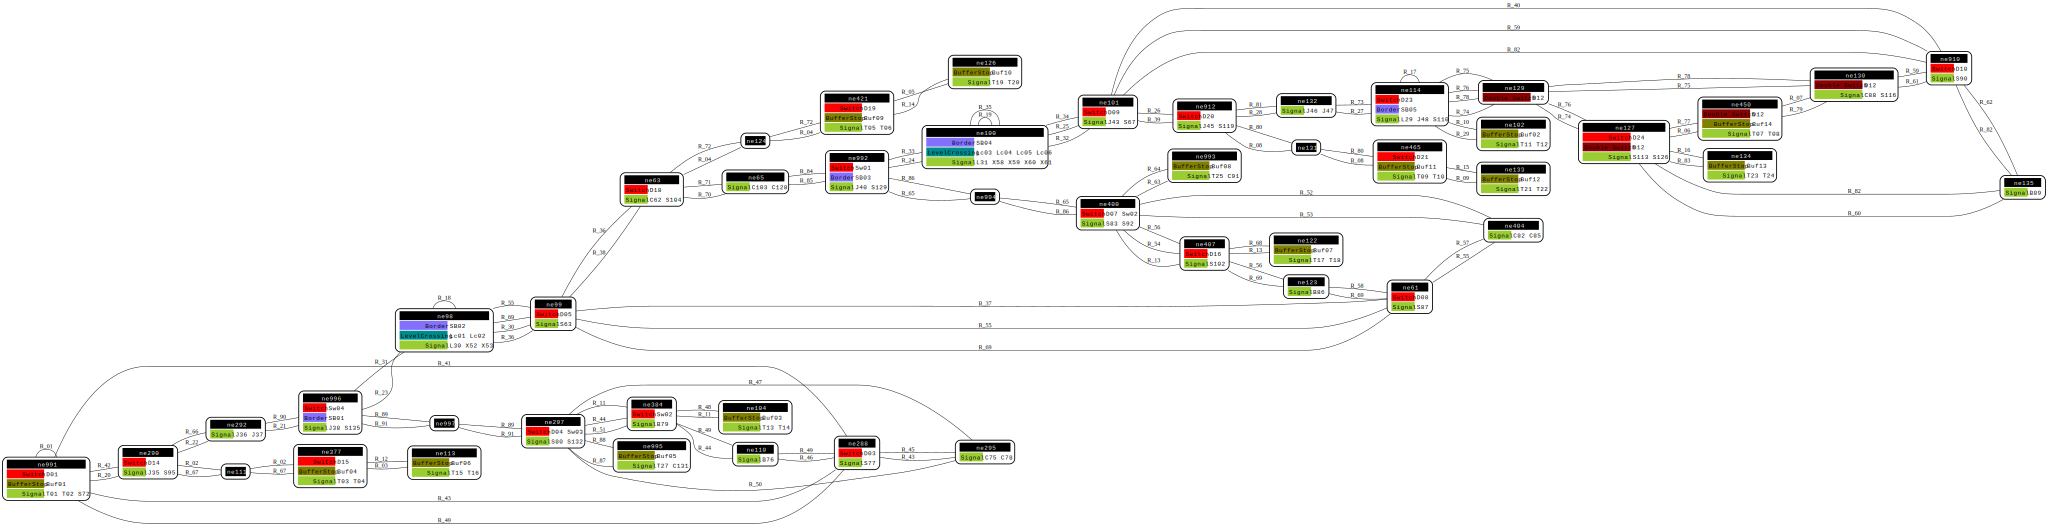
\includegraphics[width=1\textwidth]{Figuras/Graph_4}
		\centering\caption{Red de grafos generada por el RNA para el ejemplo 4.}
		\label{fig:EJ4_8}
	\end{figure}
	
	Cada nodo del grafo de la Figura \ref{fig:EJ4_8} corresponde a un \textit{netElement}. En cada nodo se listan todos los elementos ferroviarios contenidos por en \textit{netElement}. Las aristas del grafo son las rutas que los conectan. De esta manera, es posible detectar visualmente cualquier nodo aislado de la red o nodos que solo son accedidos en un sentido. Por ejemplo, si algún entre dos nodos no existe una cantidad par de rutas, entonces solamente se puede circular entre esos nodos en un solo sentido.
    \subsection{Sistema generado por el ACG}
	
	En base a la red de grafos, ilustrada en la Figura \ref{fig:EJ4_8}, el ACG determinó la siguiente cantidad de elementos, tal puede visualizarse en el Código \ref{lst:EJ4_8}.

	\begin{lstlisting}[language = {}, caption = Cantidad de elementos a implementar por el ACG, label = {lst:EJ4_8}]
	n_netElements:47
	n_switch:21
	n_doubleSwitch:1
	n_borders:5
	n_buffers:14
	n_levelCrossings:2
	n_platforms:0
	n_scissorCrossings:0
	n_signals:77
	N : 315
	M : 268
	\end{lstlisting}

	El código VHDL generado por el ACG es importado en un proyecto de Vivado, donde es sintetizado e implementado para generar el bitstream que será utilizado para programar la FPGA. La cantidad de elementos de la FPGA utilizados por el sistema post-síntesis y post-implementación, así como el porcentaje de uso de la plataforma, son detallados en la Tabla \ref{Tab:tabla_ACG_4}.
	
	\begin{table}[H]
		{
			\caption{Síntesis e implementación del ejemplo 4 generado por el ACG.}
			\label{Tab:tabla_ACG_4}
			\centering
			%\small
			%\centering
			\begin{center}
				\resizebox{0.7\textwidth}{!}{
					\begin{tabular}{ c c c c }
						\hline	
						Recursos & Síntesis & Implementación & Uso \\	
						\hline
						LUT & 13589 & 13556 & 25.54-25.48\%\\
						FF & 17256 & 17256 & 16.22\%\\
						IO & 16 & 16 & 12.80\%\\
						BUFG & 1 & 1 & 3.13\%\\
						\hline
					\end{tabular}
				}
			\end{center}
		}    
	\end{table}
	
	En este ejemplo, la cantidad de recursos utilizados es baja y el tiempo de sintetización e implementación es de 1 minuto con 39 segundos y 1 minuto con 22 segundos respectivamente.
    \subsection{Validacion del sistema}

    \lipsum[1]

    \begin{table}[!h]
        {
        \caption{Equivalencias entre las rutas 1 a 15 originales y las generadas por el RNA.}
        \label{Tab:tabla_validation_4_1}
        \centering
        %\small
            %\centering
            \begin{center}
            \resizebox{1\textwidth}{!}{
            \begin{tabular}{ c c c c }
                \hline	
                    Original & Señales & RNA & Señales \\	
                \hline
                    R$_{01}$ & S$_{15}$-S$_{24}$ & R$_{31}$ & S$_{52}$-S$_{63}$\\
                    R$_{02}$ & S$_{16}$-S$_{67}$ & R$_{32}$+R$_{89}$ & S$_{53}$-S$_{37}$\\
                    R$_{03}$ & S$_{16}$-S$_{43}$ & R$_{32}$+R$_{90}$ & S$_{53}$-S$_{79}$\\
                    R$_{04}$ & S$_{19}$-S$_{32}$ & R$_{35}$ & S$_{60}$-S$_{67}$\\
                    R$_{05}$ & S$_{20}$-S$_{11}$ & R$_{34}$+R$_{84}$ & S$_{59}$-S$_{102}$\\
                    R$_{06}$ & S$_{20}$-S$_{56}$ & R$_{34}$+R$_{85}$ & S$_{59}$-S$_{82}$\\
                    R$_{07}$ & S$_{23}$-S$_{16}$ & R$_{37}$ & S$_{62}$-S$_{53}$\\
                    R$_{08}$ & S$_{24}$-S$_{80}$ & R$_{39}$ & S$_{63}$-S$_{103}$\\
                    R$_{09}$ & S$_{24}$-S$_{52}$ & R$_{38}$+R$_{58}$ & S$_{63}$-S$_{81}$\\
                    R$_{10}$ & S$_{24}$-S$_{57}$ & R$_{38}$+R$_{59}$ & S$_{63}$-S$_{85}$\\
                    R$_{11}$ & S$_{27}$-S$_{56}$ & R$_{66}$ & S$_{90}$-S$_{82}$\\
                    R$_{12}$ & S$_{28}$-S$_{04}$ & R$_{54}$+R$_{56}$+R$_{32}$+R$_{90}$+R$_{52}$ & S$_{82}$-S$_{78}$\\
                    R$_{13}$ & S$_{28}$-S$_{19}$ & R$_{68}$+R$_{25}$ & S$_{91}$-S$_{31}$\\
                    R$_{14}$ & S$_{31}$-S$_{20}$ & R$_{27}$+R$_{26}$ & S$_{45}$-S$_{61}$\\
                    R$_{15}$ & S$_{32}$-S$_{91}$ & R$_{40}$ & S$_{67}$-S$_{112}$\\                 
                \hline
            \end{tabular}
            }
            \end{center}
        }    
    \end{table}

    \begin{table}[!h]
        {
        \caption{Equivalencias entre las rutas 16 a 30 originales y las generadas por el RNA.}
        \label{Tab:tabla_validation_4_2}
        \centering
        %\small
            %\centering
            \begin{center}
            \resizebox{1\textwidth}{!}{
            \begin{tabular}{ c c c c }
                \hline	
                    Original & Señales & RNA & Señales \\	
                \hline
                    R$_{16}$ & S$_{32}$-S$_{59}$ & R$_{41}$+R$_{63}$+R$_{78}$ & S$_{67}$-S$_{87}$\\
                    R$_{17}$ & S$_{32}$-S$_{60}$ & R$_{41}$+R$_{65}$ & S$_{67}$-S$_{88}$\\
                    R$_{18}$ & S$_{35}$-S$_{01}$ & R$_{69}$+R$_{22}$+R$_{24}$+R$_{31}$+R$_{39}$+R$_{74}$+R$_{83}$+R$_{25}$+R$_{35}$+R$_{41}$+R$_{63}$+R$_{78}$ & S$_{94}$-S$_{87}$\\
                    R$_{19}$ & S$_{39}$-S$_{43}$ & R$_{86}$ & S$_{124}$-S$_{79}$\\
                    R$_{20}$ & S$_{44}$-S$_{04}$ & R$_{45}$+R$_{52}$ & S$_{75}$-S$_{78}$\\
                    R$_{21}$ & S$_{45}$-S$_{01}$ & R$_{48}$+R$_{88}$+R$_{24}$+R$_{31}$+R$_{39}$+R$_{74}$+R$_{83}$+R$_{25}$+R$_{35}$+R$_{41}$+R$_{63}$+R$_{78}$ & S$_{77}$-S$_{87}$\\
                    R$_{22}$ & S$_{46}$-S$_{63}$ & R$_{50}$+R$_{42}$+R$_{47}$ & S$_{78}$-S$_{75}$\\
                    R$_{23}$ & S$_{46}$-S$_{09}$ & R$_{50}$+R$_{43}$+R$_{69}$ & S$_{78}$-S$_{36}$\\
                    R$_{24}$ & S$_{47}$-S$_{40}$ & R$_{48}$ & S$_{77}$-S$_{125}$\\
                    R$_{25}$ & S$_{52}$-S$_{28}$ & R$_{53}$ & S$_{81}$-S$_{91}$\\
                    R$_{26}$ & S$_{56}$-S$_{58}$ & R$_{54}$ & S$_{82}$-S$_{84}$\\
                    R$_{27}$ & S$_{56}$-S$_{03}$ & R$_{55}$ & S$_{82}$-S$_{101}$\\
                    R$_{28}$ & S$_{57}$-S$_{76}$ & R$_{57}$+R$_{55}$ & S$_{85}$-S$_{101}$\\
                    R$_{29}$ & S$_{58}$-S$_{16}$ & R$_{56}$ & S$_{84}$-S$_{53}$\\
                    R$_{30}$ & S$_{59}$-S$_{87}$ & R$_{60}$+R$_{41}$+R$_{63}$ & S$_{87}$-S$_{29}$\\              
                \hline
            \end{tabular}
            }
            \end{center}
        }    
    \end{table}

    \begin{table}[!h]
        {
        \caption{Equivalencias entre las rutas 31 a 45 originales y las generadas por el RNA.}
        \label{Tab:tabla_validation_4_3}
        \centering
        %\small
            %\centering
            \begin{center}
            \resizebox{1\textwidth}{!}{
            \begin{tabular}{ c c c c }
                \hline	
                    Original & Señales & RNA & Señales \\	
                \hline
                    R$_{31}$ & S$_{59}$-S$_{06}$ & R$_{60}$+R$_{26}$+R$_{34}$+R$_{84}$+R$_{73}$+R$_{37}$+R$_{32}$+R$_{89}$+R$_{23}$+R$_{70}$ & S$_{87}$-S$_{03}$\\
                    R$_{32}$ & S$_{60}$-S$_{99}$ & R$_{61}$+R$_{77}$ & S$_{88}$-S$_{119}$\\
                    R$_{33}$ & S$_{62}$-S$_{04}$ & R$_{11}$+R$_{52}$ & S$_{14}$-S$_{78}$\\
                    R$_{34}$ & S$_{63}$-S$_{01}$ & R$_{45}$+R$_{88}$+R$_{24}$+R$_{31}$+R$_{39}$+R$_{74}$+R$_{83}$+R$_{35}$+R$_{35}$+R$_{41}$+R$_{63}$+R$_{78}$ & S$_{75}$-S$_{87}$\\
                    R$_{35}$ & S$_{67}$-S$_{09}$ & R$_{89}$ & S$_{128}$-S$_{37}$\\
                    R$_{36}$ & S$_{68}$-S$_{08}$ & R$_{43}$ & S$_{71}$-S$_{94}$\\
                    R$_{37}$ & S$_{74}$-S$_{76}$ & R$_{13}$+R$_{55}$ & S$_{18}$-S$_{101}$\\
                    R$_{38}$ & S$_{75}$-S$_{16}$ & R$_{57}$+R$_{54}$+R$_{56}$ & S$_{85}$-S$_{53}$\\
                    R$_{39}$ & S$_{76}$-S$_{28}$ & R$_{71}$+R$_{13}$ & S$_{101}$-S$_{91}$\\
                    R$_{40}$ & S$_{80}$-S$_{10}$ & R$_{31}$+R$_{39}$ & S$_{52}$-S$_{103}$\\
                    R$_{41}$ & S$_{83}$-S$_{12}$ & R$_{05}$ & S$_{06}$-S$_{19}$\\
                    R$_{42}$ & S$_{84}$-S$_{85}$ & R$_{75}$ & S$_{103}$-S$_{05}$\\
                    R$_{43}$ & S$_{85}$-S$_{05}$ & R$_{75}$ & S$_{103}$-S$_{05}$\\
                    R$_{44}$ & S$_{86}$-S$_{87}$ & R$_{28}$ & S$_{46}$-S$_{29}$\\
                    R$_{45}$ & S$_{87}$-S$_{08}$ & R$_{77}$+R$_{81}$+R$_{26}$+R$_{34}$+R$_{84}$+R$_{73}$+R$_{37}$+R$_{32}$+R$_{89}$+R$_{23}$ & S$_{109}$-S$_{35}$\\              
                \hline
            \end{tabular}
            }
            \end{center}
        }    
    \end{table}

    \begin{table}[!h]
        {
        \caption{Equivalencias entre las rutas 46 a 60 originales y las generadas por el RNA.}
        \label{Tab:tabla_validation_4_4}
        \centering
        %\small
            %\centering
            \begin{center}
            \resizebox{1\textwidth}{!}{
            \begin{tabular}{ c c c c }
                \hline	
                    Original & Señales & RNA & Señales \\	
                \hline
                    R$_{46}$ & S$_{89}$-S$_{31}$ & R$_{29}$ & S$_{47}$-S$_{45}$\\
                    R$_{47}$ & S$_{90}$-S$_{89}$ & R$_{76}$ & S$_{109}$-S$_{47}$\\
                    R$_{48}$ & S$_{91}$-S$_{93}$ & R$_{40}$ & S$_{67}$-S$_{112}$\\
                    R$_{49}$ & S$_{93}$-S$_{86}$ & R$_{80}$ & S$_{112}$-S$_{46}$\\
                    R$_{50}$ & S$_{93}$-S$_{95}$ & R$_{79}$ & S$_{112}$-S$_{09}$\\
                    R$_{51}$ & S$_{94}$-S$_{13}$ & R$_{09}$ & S$_{10}$-S$_{21}$\\
                    R$_{52}$ & S$_{95}$-S$_{96}$ & R$_{79}$ & S$_{112}$-S$_{09}$\\
                    R$_{53}$ & S$_{96}$-S$_{07}$ & R$_{08}$+R$_{27}$+R$_{26}$+R$_{34}$+R$_{84}$+R$_{73}$+R$_{37}$+R$_{32}$+R$_{89}$+R$_{23}$+R$_{21}$ & S$_{10}$-S$_{01}$\\
                    R$_{54}$ & S$_{97}$-S$_{99}$ & R$_{16}$+R$_{77}$ & S$_{24}$-S$_{119}$\\
                    R$_{55}$ & S$_{98}$-S$_{20}$ & R$_{61}$+R$_{77}$+R$_{81}$+R$_{26}$ & S$_{88}$-S$_{61}$\\
                    R$_{56}$ & S$_{99}$-S$_{87}$ & R$_{82}$+R$_{16}$ & S$_{119}$-S$_{29}$\\
                    R$_{57}$ & S$_{99}$-S$_{06}$ & R$_{81}$+R$_{26}$+R$_{34}$+R$_{84}$+R$_{73}$+R$_{37}$+R$_{32}$+R$_{89}$+R$_{23}$+R$_{70}$& S$_{119}$-S$_{03}$\\
                    R$_{58}$ & S$_{40}$-S$_{02}$ & R$_{88}$+R$_{24}$+R$_{31}$+R$_{39}$+R$_{74}$ & S$_{125}$-S$_{121}$\\
                    R$_{59}$ & S$_{40}$-S$_{15}$ & R$_{88}$+R$_{24}$ & S$_{125}$-S$_{30}$\\
                    R$_{60}$ & S$_{43}$-S$_{45}$ & R$_{51}$ & S$_{87}$-S$_{43}$\\              
                \hline
            \end{tabular}
            }
            \end{center}
        }    
    \end{table}

    \begin{table}[!h]
        {
        \caption{Equivalencias entre las rutas 61 a 77 originales y las generadas por el RNA.}
        \label{Tab:tabla_validation_4_5}
        \centering
        %\small
            %\centering
            \begin{center}
            \resizebox{1\textwidth}{!}{
            \begin{tabular}{ c c c c }
                \hline	
                    Original & Señales & RNA & Señales \\	
                \hline
                    R$_{61}$ & S$_{43}$-S$_{46}$ & R$_{52}$ & S$_{79}$-S$_{78}$\\
                    R$_{62}$ & S$_{01}$-S$_{20}$ & R$_{60}$+R$_{26}$ & S$_{87}$-S$_{43}$\\
                    R$_{63}$ & S$_{02}$-S$_{19}$ & R$_{83}$+R$_{25}$ & S$_{121}$-S$_{31}$\\
                    R$_{64}$ & S$_{03}$-S$_{75}$ & R$_{72}$+R$_{31}$+R$_{38}$+R$_{59}$ & S$_{101}$-S$_{85}$\\
                    R$_{65}$ & S$_{03}$-S$_{11}$ & R$_{71}$+R$_{13}$+R$_{68}$+R$_{84}$ & S$_{101}$-S$_{102}$\\
                    R$_{66}$ & S$_{04}$-S$_{40}$ & R$_{49}$+R$_{11}$ & S$_{78}$-S$_{125}$\\
                    R$_{67}$ & S$_{06}$-S$_{10}$ & R$_{02}$+R$_{69}$+R$_{22}$+R$_{24}$+R$_{31}$+R$_{39}$ & S$_{04}$-S$_{103}$\\
                    R$_{68}$ & S$_{06}$-S$_{35}$ & R$_{02}$ & S$_{04}$-S$_{35}$\\
                    R$_{69}$ & S$_{07}$-S$_{68}$ & R$_{43}$ & S$_{71}$-S$_{94}$\\
                    R$_{70}$ & S$_{07}$-S$_{47}$ & R$_{42}$+R$_{46}$ & S$_{71}$-S$_{77}$\\
                    R$_{71}$ & S$_{07}$-S$_{44}$ & R$_{42}$+R$_{47}$ & S$_{71}$-S$_{75}$\\
                    R$_{72}$ & S$_{08}$-S$_{15}$ & R$_{69}$+R$_{22}$+R$_{24}$ & S$_{94}$-S$_{30}$\\
                    R$_{73}$ & S$_{08}$-S$_{03}$ & R$_{69}$+R$_{22}$+R$_{24}$+R$_{31}$+R$_{38}$+R$_{58}$+R$_{53}$+R$_{55}$ & S$_{94}$-S$_{101}$\\
                    R$_{74}$ & S$_{09}$-S$_{35}$ & R$_{23}$ & S$_{37}$-S$_{35}$\\
                    R$_{75}$ & S$_{10}$-S$_{02}$ & R$_{74}$ & S$_{103}$-S$_{121}$\\
                    R$_{76}$ & S$_{10}$-S$_{84}$ & R$_{75}$ & S$_{103}$-S$_{05}$\\
                    R$_{77}$ & S$_{11}$-S$_{23}$ & R$_{73}$ & S$_{102}$-S$_{62}$\\            
                \hline
            \end{tabular}
            }
            \end{center}
        }    
    \end{table}
	%\chapter{Ejemplo 5}

	\label{sec:ejemplo_5}
	
    \subsection{Topología ferroviaria original}

	El quinto ejemplo, ilustrado en la Figura \ref{fig:EJ5_1}, es una topología de dos vías principales paralelas y disconexas, con sus correspondientes desvíos para poder operar cada línea en ambos sentidos. La primera vía principal, la vía superior, utiliza los cambios de vías Sw01 y Sw02 para permitir circular dos formaciones en sentido contrario. En tanto que la segunda vía principal, la vía inferior, utiliza los cambios de vías Sw03 y Sw04 para el mismo fin. El objetivo de este ejemplo fue comprobar el funcionamiento del RNA con una topología de dos bypasses independientes y disconexos.
	
	\begin{figure}[h]
		\centering
		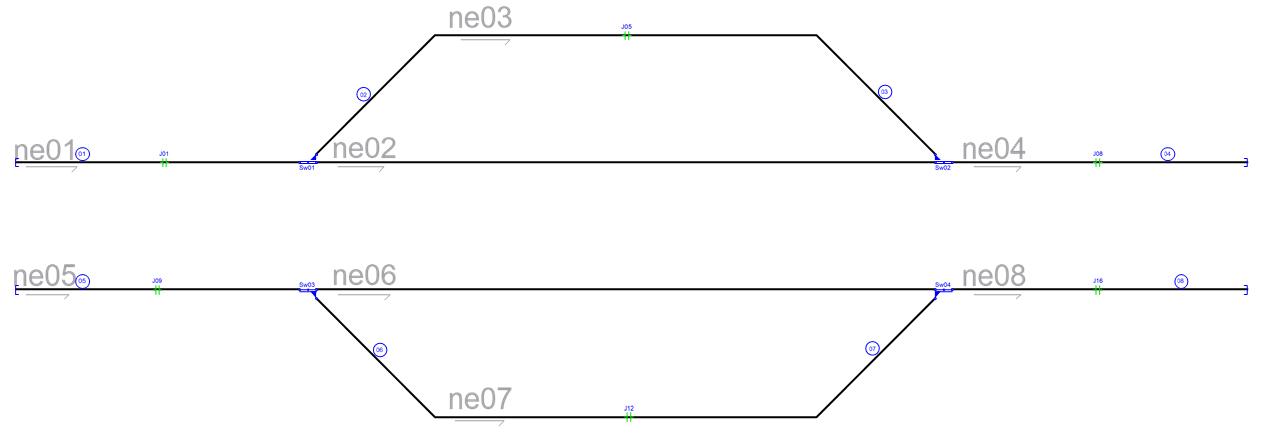
\includegraphics[width=1\textwidth]{resultados-obtenidos/ejemplo5/images/5_empty.png}
		\centering\caption{Topología ferroviaria del ejemplo 5 sin señalamiento.}
		\label{fig:EJ5_1}
	\end{figure}
	
	Para incrementar la dificultad del análisis y obtener resultados mas completos, todos los finales de vías absolutos. Además, se incluyeron junturas entre los finales de vías y los cambios de vías.

    \subsection{Señalamiento original}

    \lipsum[1]
    
    \begin{table}[!h]
        {
        \caption{Tabla de enclavamiento original del ejemplo 5.}
        \label{Tab:tabla_original_5}
        \centering
        \resizebox{1\textwidth}{!}{
            \begin{tabular}{ c c c c c c c }
                \hline	
                    Ruta & Inicio & Final & Cambio & Plataforma & Cruce & netElement \\	
                \hline
                    R$_{01}$  & S$_{01}$ & S$_{06}$ & Sw$_{01}^{N}$ & - & - & ne$_{01}$-ne$_{02}$\\
                    R$_{02}$  & S$_{05}$ & S$_{13}$ & Sw$_{01}^{N}$ & - & - & ne$_{02}$-ne$_{01}$\\
                    R$_{03}$  & S$_{01}$ & S$_{03}$ & Sw$_{01}^{R}$ & - & - & ne$_{01}$-ne$_{03}$\\
                    R$_{04}$  & S$_{04}$ & S$_{13}$ & Sw$_{01}^{R}$ & - & - & ne$_{03}$-ne$_{01}$\\
                    R$_{05}$  & S$_{02}$ & S$_{04}$ & Sw$_{02}^{R}$ & - & - & ne$_{04}$-ne$_{02}$\\
                    R$_{06}$  & S$_{06}$ & S$_{15}$ & Sw$_{02}^{N}$ & - & - & ne$_{02}$-ne$_{04}$\\
                    R$_{07}$  & S$_{02}$ & S$_{05}$ & Sw$_{02}^{N}$ & - & - & ne$_{04}$-ne$_{03}$\\
                    R$_{08}$  & S$_{03}$ & S$_{15}$ & Sw$_{02}^{R}$ & - & - & ne$_{03}$-ne$_{04}$\\
                    R$_{09}$  & S$_{07}$ & S$_{11}$ & Sw$_{03}^{N}$ & - & - & ne$_{05}$-ne$_{06}$\\
                    R$_{10}$  & S$_{10}$ & S$_{14}$ & Sw$_{03}^{N}$ & - & - & ne$_{06}$-ne$_{05}$\\
                    R$_{11}$  & S$_{07}$ & S$_{09}$ & Sw$_{03}^{R}$ & - & - & ne$_{05}$-ne$_{07}$\\
                    R$_{12}$  & S$_{08}$ & S$_{14}$ & Sw$_{03}^{R}$ & - & - & ne$_{07}$-ne$_{05}$\\
                    R$_{13}$  & S$_{12}$ & S$_{10}$ & Sw$_{04}^{N}$ & - & - & ne$_{08}$-ne$_{06}$\\
                    R$_{14}$  & S$_{11}$ & S$_{16}$ & Sw$_{04}^{N}$ & - & - & ne$_{06}$-ne$_{08}$\\
                    R$_{15}$  & S$_{12}$ & S$_{08}$ & Sw$_{04}^{R}$ & - & - & ne$_{08}$-ne$_{07}$\\
                    R$_{16}$  & S$_{09}$ & S$_{16}$ & Sw$_{04}^{R}$ & - & - & ne$_{07}$-ne$_{08}$\\
                \hline
            \end{tabular}
        }
     }
    \end{table}
    \subsection{Generación de señalamiento paso a paso}

	Al ejecutar el RNA, primero detectará todos los \textit{netElements}, sus coordenadas iniciales y finales en la topología, y el sentido en el que fueron definidas. El resultado obtenido se muestra en el Cóodigo \ref{lst:EJ5_1}.
	
	\begin{lstlisting}[language = {}, caption = Detección de \textit{netElements} por parte del RNA , label = {lst:EJ5_1}]
		###### Starting Railway Network Analyzer #####
		Reading .railML file
		Creating railML object
		Analyzing railML object
		Analyzing graph
		ne01 [-1451, -150] [-763, -150] >>
		ne02 [-763, -150] [736, -150] >>
		ne03 [-763, -150] [736, -150] >>
		ne04 [736, -150] [1451, -150] >>
		ne05 [-1451, -450] [-763, -450] >>
		ne06 [-763, -450] [736, -450] >>
		ne07 [-763, -450] [736, -450] >>
		ne08 [736, -450] [1451, -450] >>
		The network is not connected
	\end{lstlisting}
	
	Por ejemplo, el \textit{netElement} ne08 inicia en la coordenada (736;-450) y finaliza en la coordenada (1451;-450). El símbolo $>>$ indica que ne08 se encuentra definido de izquierda a derecha, ya que la componente x de la coordenada final es mayor a la de la coordenada inicial, teniendo la misma componente y. Además, se puede comprobar que la lista obtenida en consistente con la Figura \ref{fig:EJ5_2}. Por ejemplo, ne01, ne02 y ne03 comparten la coordenada (736;-450), que coincide con la coordenada del cambio de vías Sw01.
	
	A continuación, el RNA detectará la infraestructura ferroviaria, las curvas peligrosas y los puntos medios de los netElements que el RNA considera demasiado largos. El resultado de este proceso se puede visualizar en el Código \ref{lst:EJ5_2} y puede leerse también en el archivo Infrastructure.RNA.
	
	\begin{lstlisting}[language = {}, caption = Detección de puntos críticos por parte del RNA , label = {lst:EJ5_2}]
	Analyzing infrastructure --> Infrastructure.RNA
	Detecting Danger --> Safe_points.RNA
	ne01 has a RailJoint[J01] @ [-1101, -150]     
	ne02 has a Middle point @ [-548.9, -150]      
	ne02 has a Middle point @ [-334.7, -150]      
	ne02 has a Middle point @ [-120.6, -150]
	ne02 has a Middle point @ [93.6, -150]
	ne02 has a Middle point @ [307.7, -150]
	ne02 has a Middle point @ [521.9, -150]
	ne03 has a RailJoint[J05] @ [-11, 150]
	ne03 has a Curve(3 lines) @ [[-463, 150], [436, 150]]
	ne04 has a RailJoint[J08] @ [1100, -150]
	ne05 has a RailJoint[J09] @ [-1118, -450]
	ne06 has a Middle point @ [-548.9, -450]
	ne06 has a Middle point @ [-334.7, -450]
	ne06 has a Middle point @ [-120.6, -450]
	ne06 has a Middle point @ [93.6, -450]
	ne06 has a Middle point @ [307.7, -450]
	ne06 has a Middle point @ [521.9, -450]
	ne07 has a RailJoint[J12] @ [-5, -750]
	ne07 has a Curve(3 lines) @ [[-463, -750], [436, -750]]
	ne08 has a RailJoint[J16] @ [1100, -450]
	\end{lstlisting}
	
	Una vez que el RNA detectó cada punto crítico de la red ferroviaria, procede a generar el señalamiento. El orden de generación no es importante, pero para poder describirlo de forma consistente se iniciará generando el señalamiento para proteger los finales de vías, las junturas entre rieles, las plataformas, los cruces de vía y los cambios de vías. Luego se procederá a mostrar el señalamiento pre y post simplificación. Las señales generadas para proteger los finales de vías relativos y absolutos son ilustradas en la Figura \ref{fig:EJ5_3}.
	
	\begin{figure}[H]
		\centering
		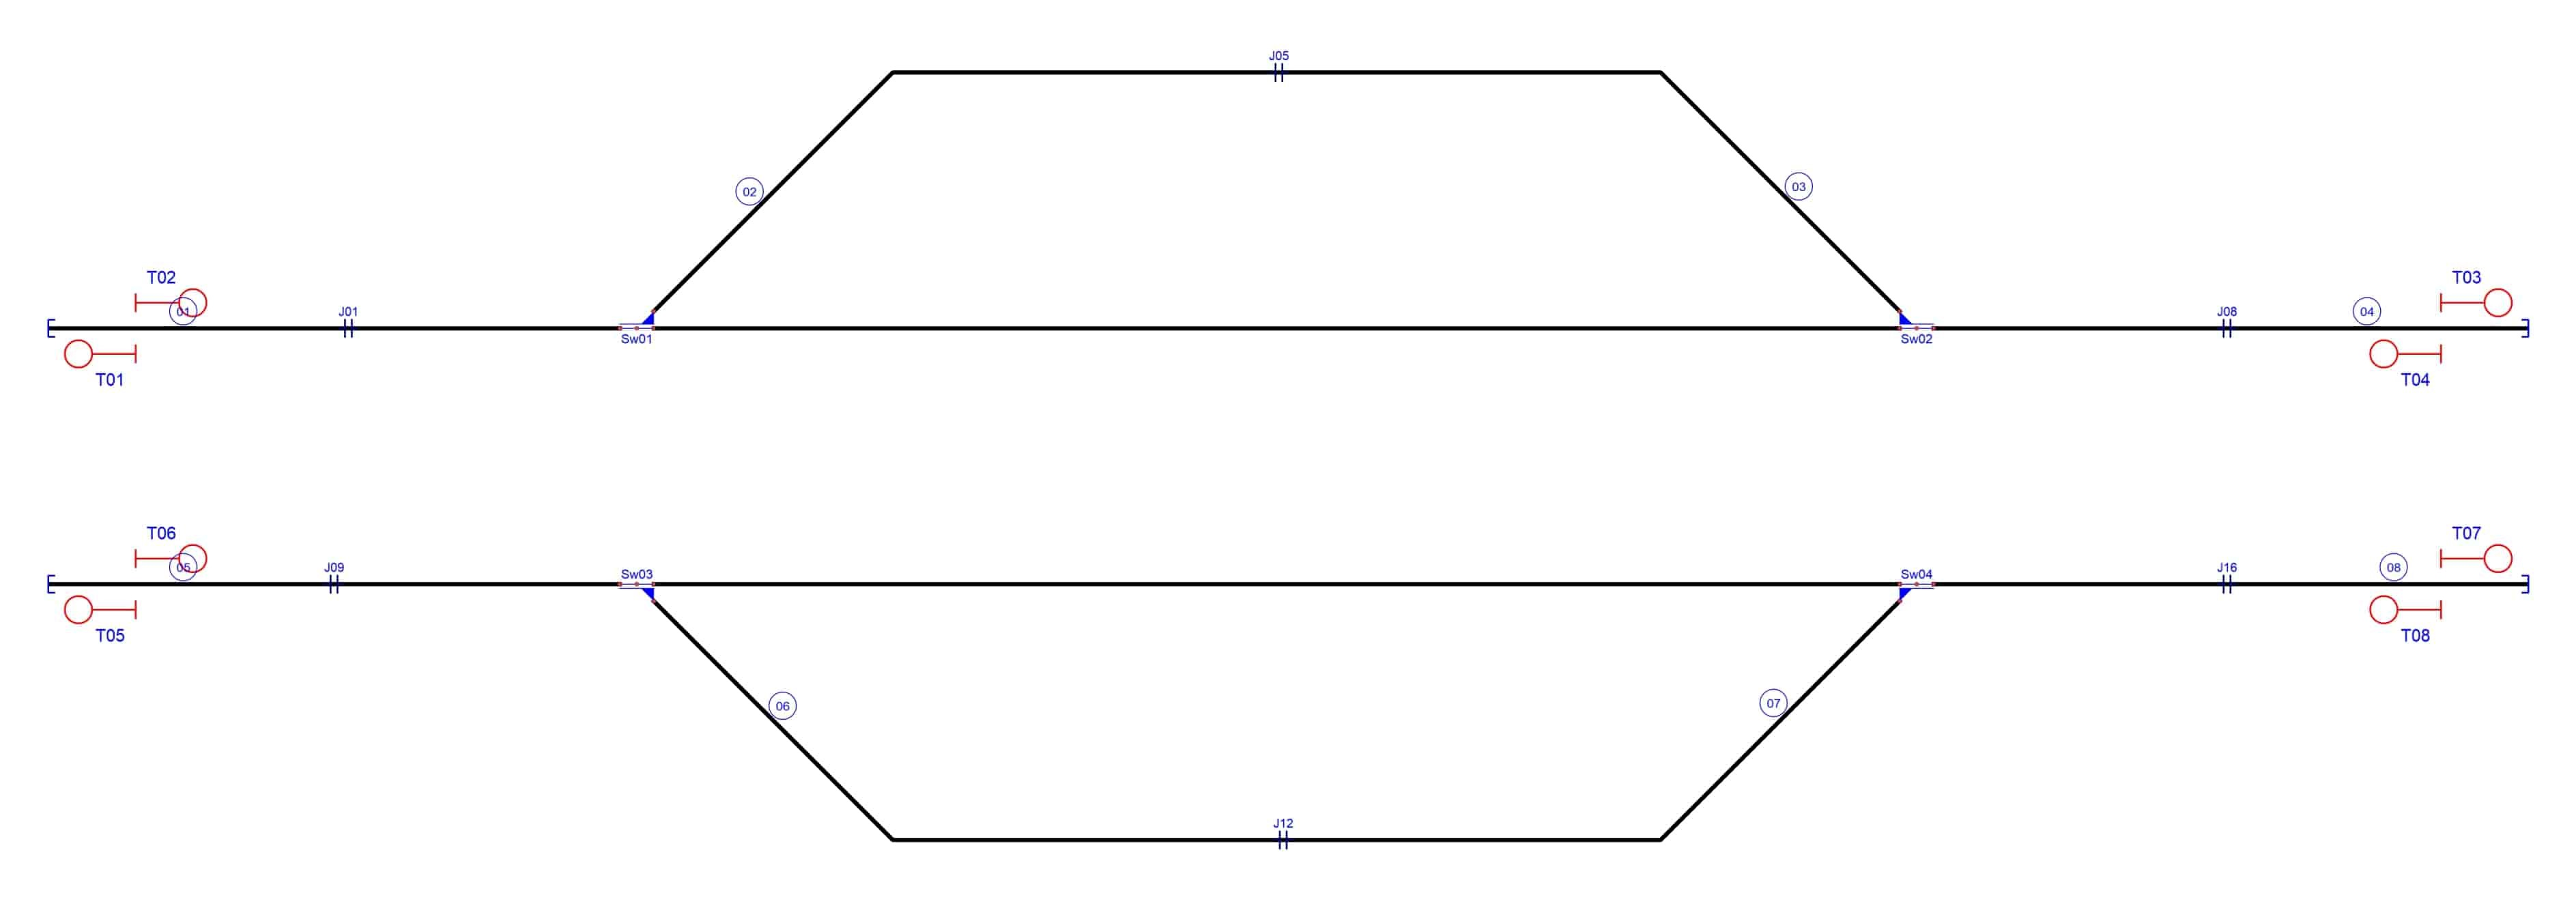
\includegraphics[width=1\textwidth]{resultados-obtenidos/ejemplo5/images/5_step1.png}
		\centering\caption{Señalamiento generado por el RNA para proteger el fin de vía.}
		\label{fig:EJ5_3}
	\end{figure}
	
	Los finales de vías absolutos son protegidos por las señales de parada T01, T03, T05 y T07, y las señales de partida son T02, T04, T06 y T08. No existen finales de vías relativos que proteger.
	
	La Figura \ref{fig:EJ5_4} ilustra la generación de señales destinadas a proteger las junturas entre los rieles. Las señales generadas son todas las señales entre J09 y J20, indicadas en color rojo.
	
	\begin{figure}[H]
		\centering
		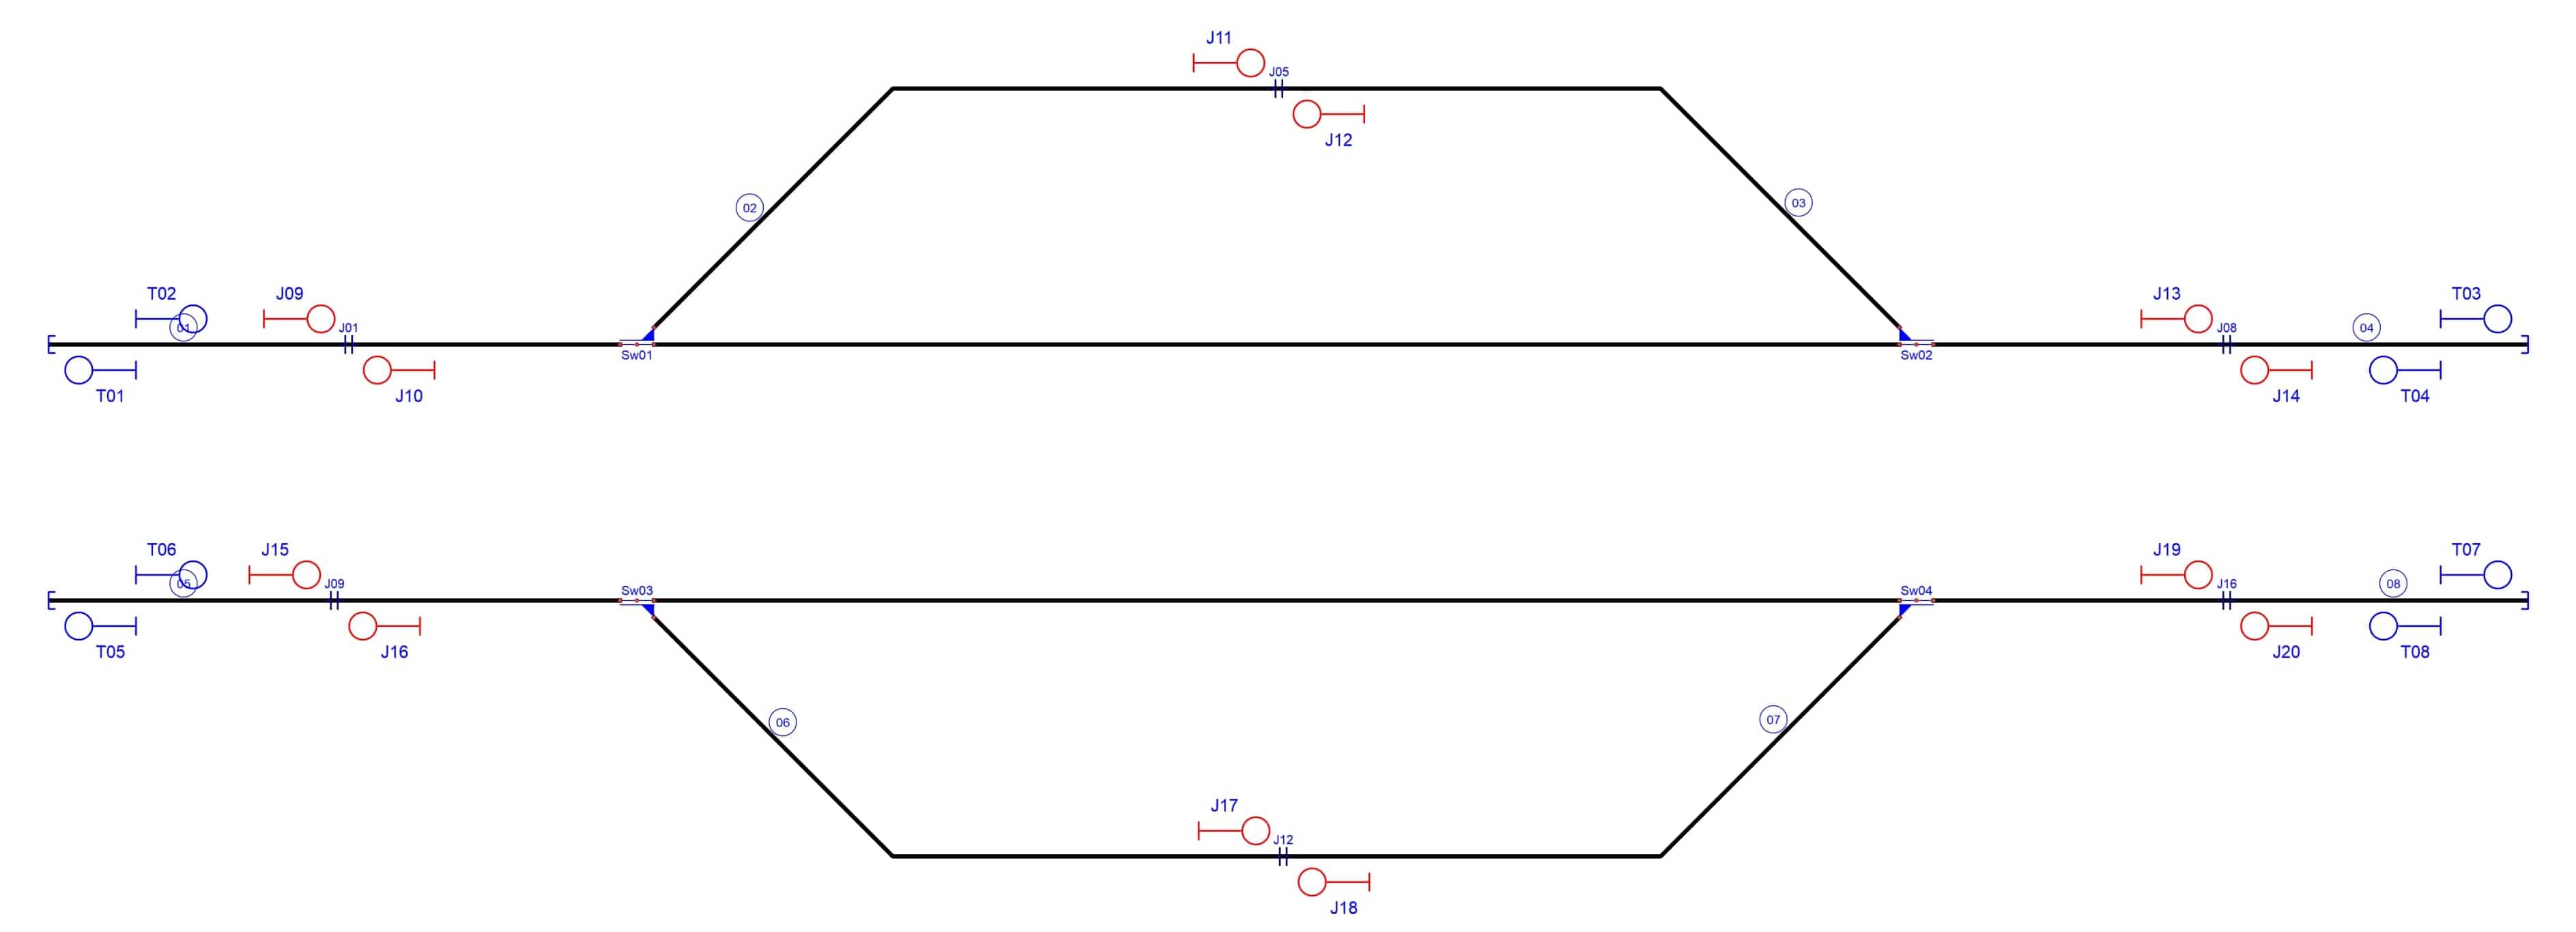
\includegraphics[width=1\textwidth]{resultados-obtenidos/ejemplo5/images/5_step2.png}
		\centering\caption{Señalamiento generado por el RNA para proteger las junturas.}
		\label{fig:EJ5_4}
	\end{figure}
	
	Al generar el señalamiento para proteger la infraestructura, tal como se explicó en la Sección \ref{sec:horizontal}, el Algoritmo \ref{alg:horizontal} simplificará las señales entre dos elementos ferroviarios si no existe espacio suficiente entre ellos. El señalamiento generado para proteger las plataformas y los cruces de vía se ilustra en rojo en la Figura \ref{fig:EJ5_5}. Al no existir plataformas o cruces de vías que proteger, ninguna señal fue generada por el RNA.
	
	\begin{figure}[H]
		\centering
		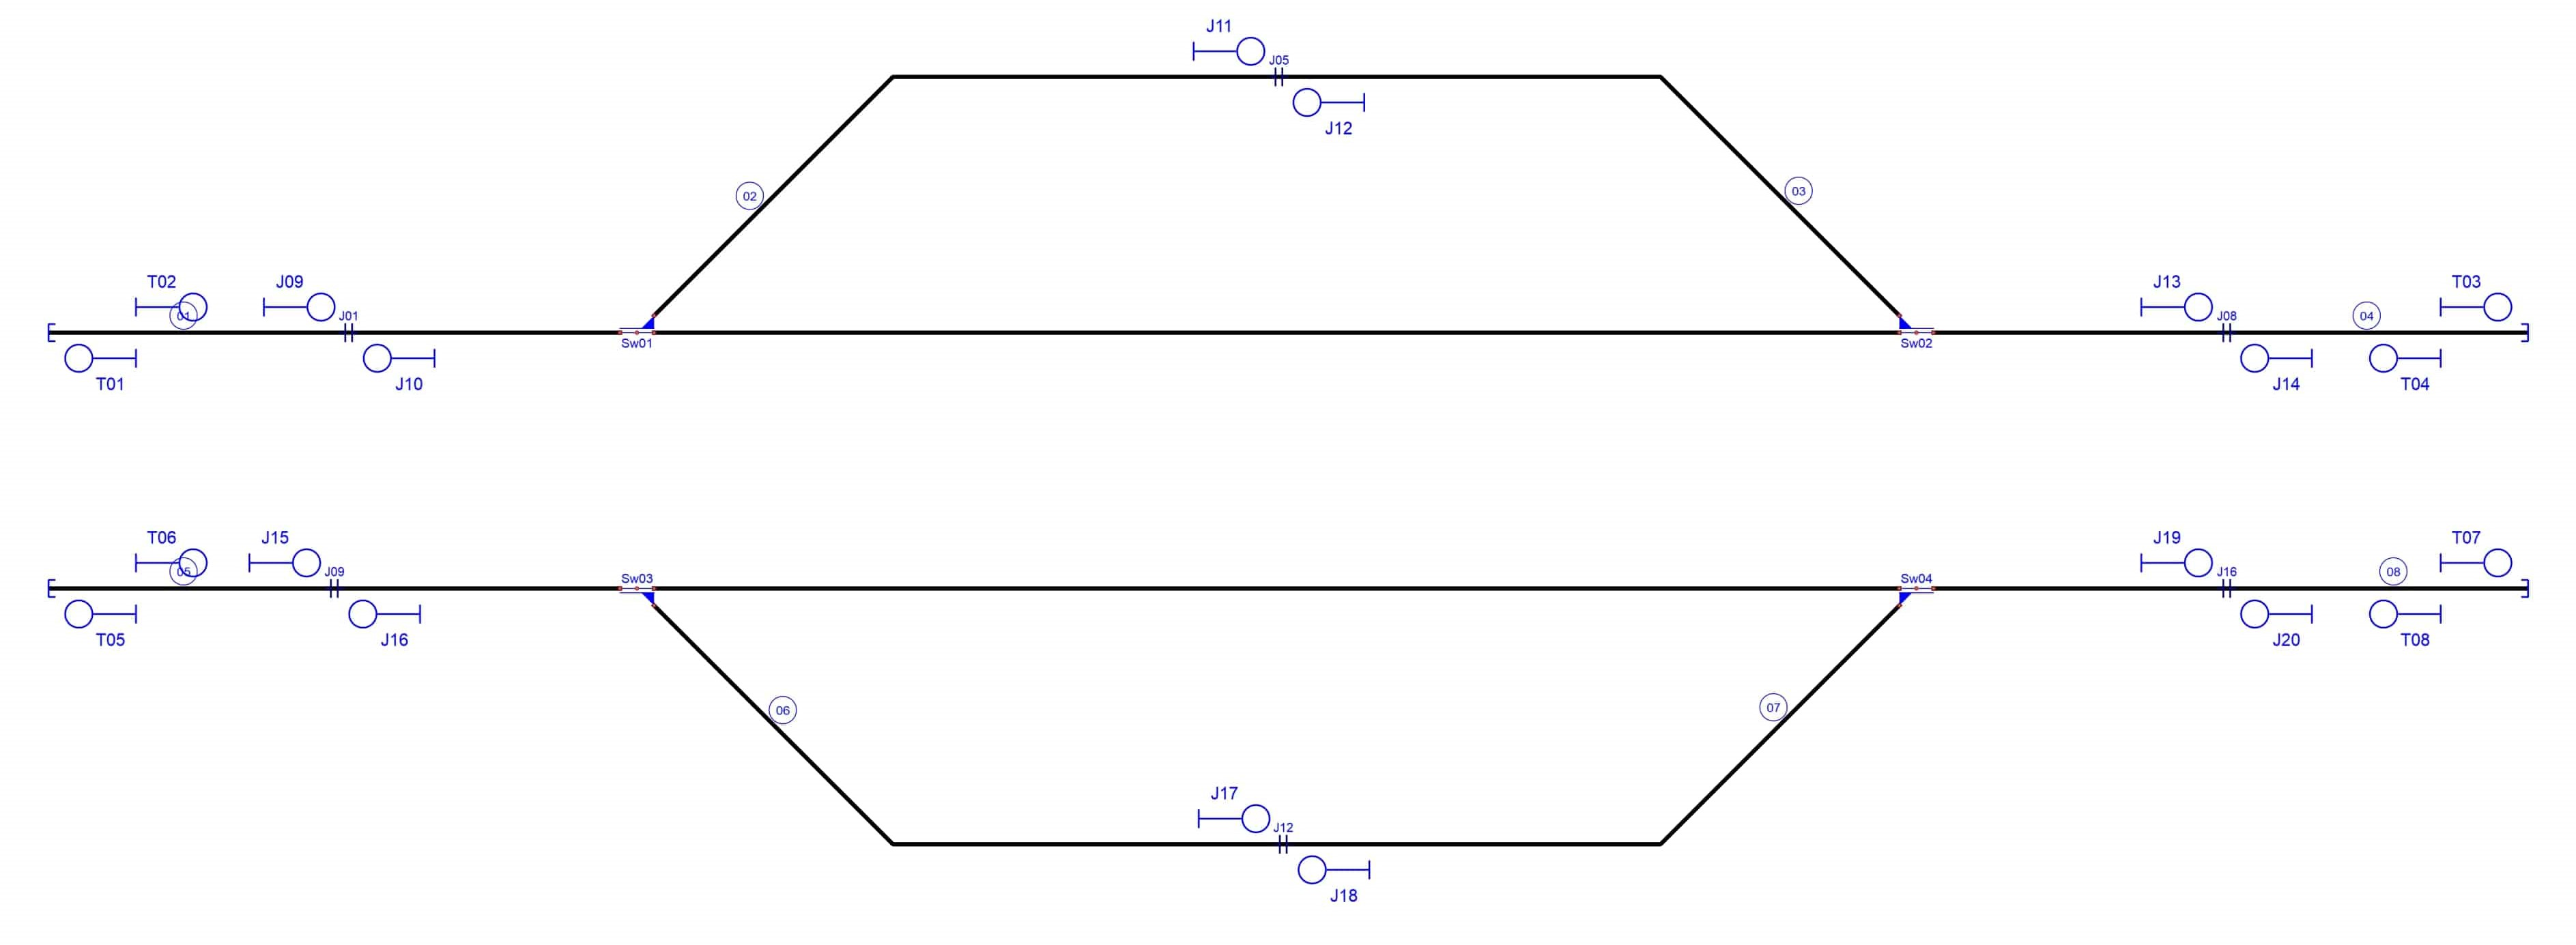
\includegraphics[width=1\textwidth]{resultados-obtenidos/ejemplo5/images/5_step3.png}
		\centering\caption{Señalamiento generado por el RNA para proteger plataformas y cruces de vía.}
		\label{fig:EJ5_5}
	\end{figure}
	
	El RNA generó las señales C21, S23, B26 y H24 para proteger el cambio de vías Sw02; las señales C25, S27, B22 y H28 para proteger el cambio de vías Sw02; las señales C29, S31. B34 y H32 para proteger el cambio de vías Sw03 y las señales C33, S35, B30 y H36 para proteger el cambio de vías Sw04. Las señales mencionadas se encuentran resaltadas en rojo en la Figura \ref{fig:EJ5_6}.
	
	\begin{figure}[H]
		\centering
		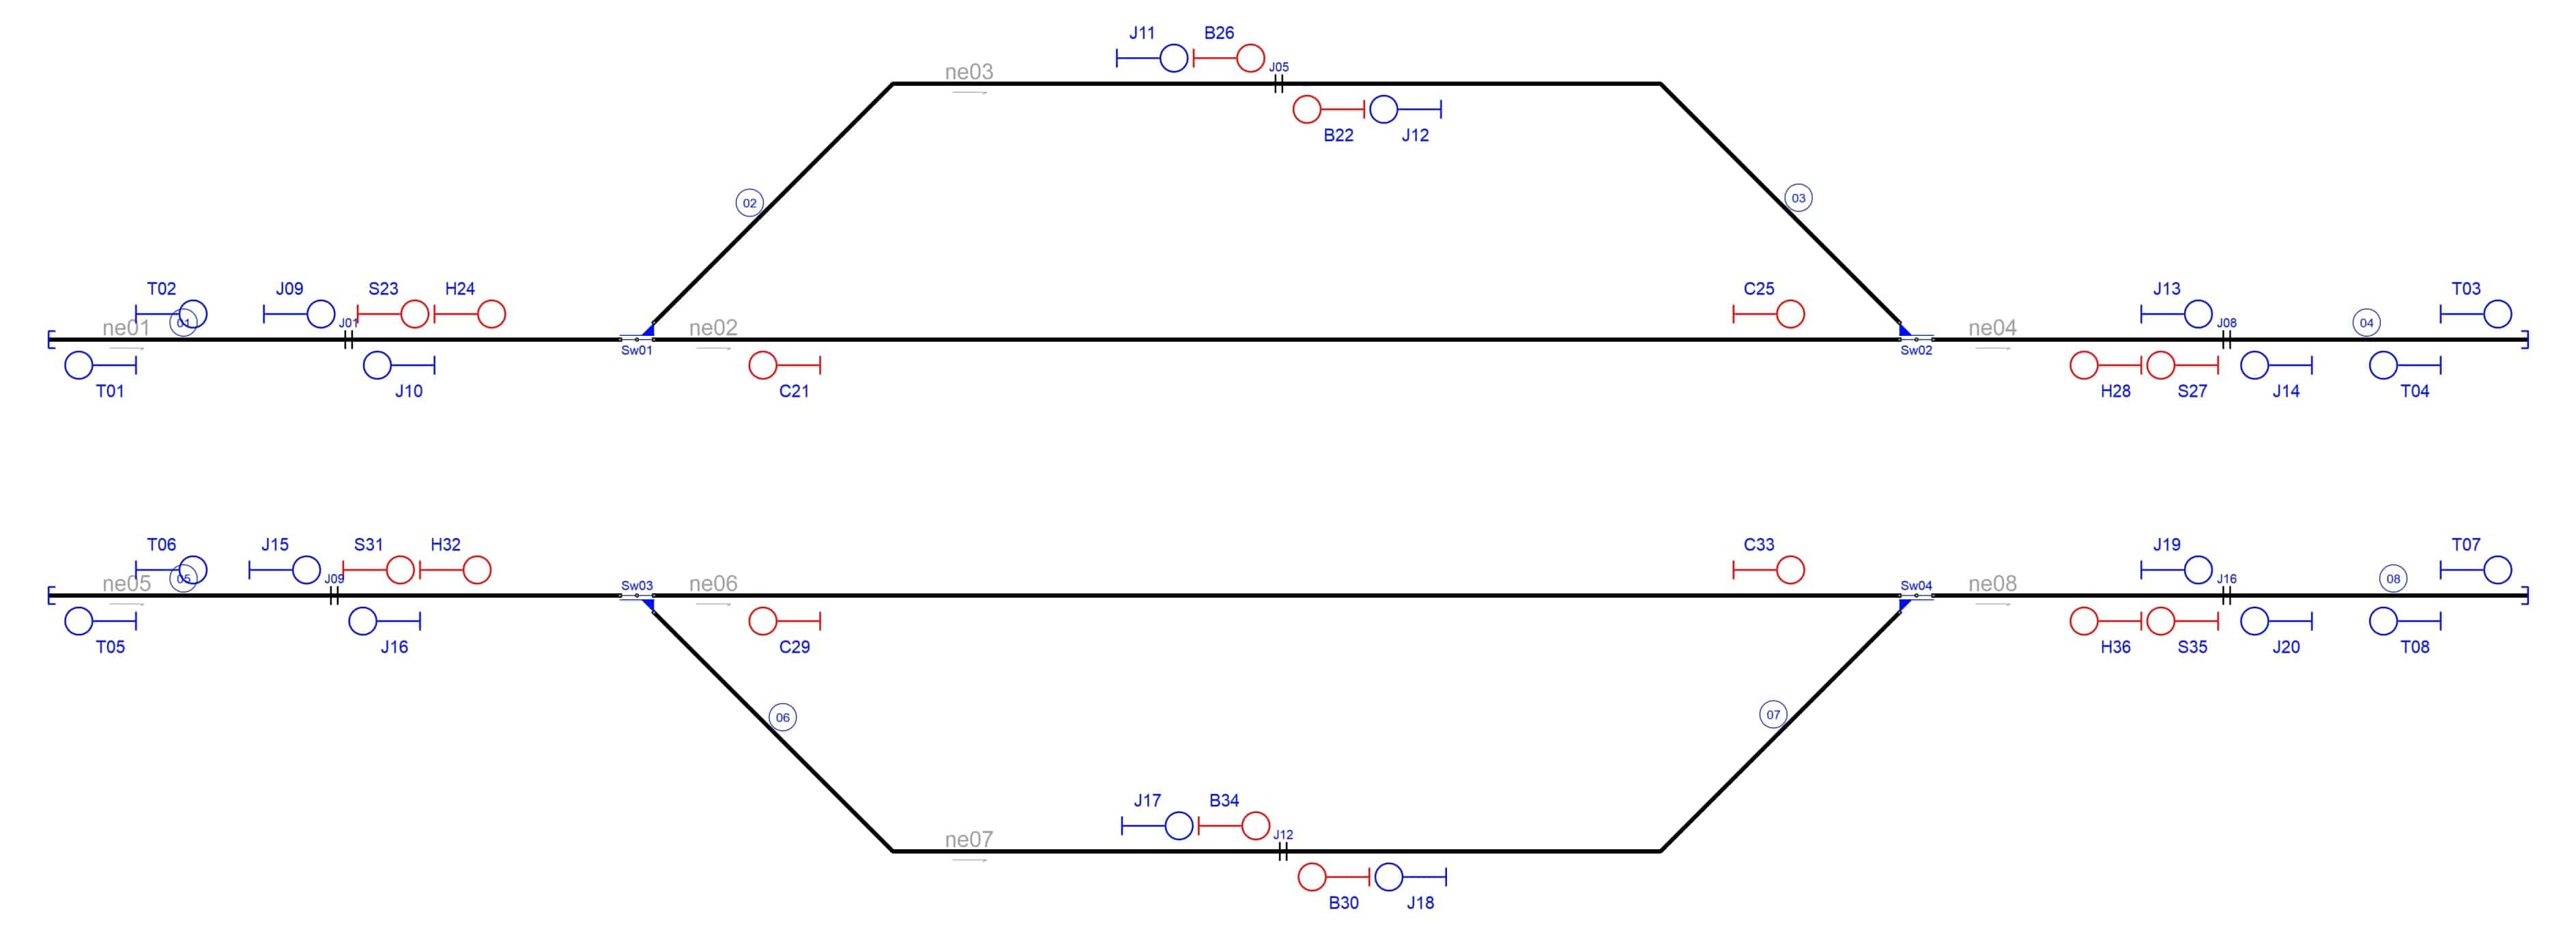
\includegraphics[width=1\textwidth]{resultados-obtenidos/ejemplo5/images/5_step4.png}
		\centering\caption{Señalamiento generado por el RNA para proteger los cambios de vías.}
		\label{fig:EJ5_6}
	\end{figure}
	
	Una vez obtenido todo el señalamiento, el RNA procede a simplificar las señales redundantes, repetidas o cuyas funciones o ubicaciones se superponen entre sí. El proceso de simplificación de señales fue explicado en la Sección \ref{sec:simplificacion}. En este ejemplo, el Algoritmo \ref{alg:vertical} de herencia vertical no fue aplicado, al no cumplirse las condiciones de aplicación.
	
	Las señales simplificadas al aplicar el Algoritmo \ref{alg:horizontal} de herencia horizontal son: J09, J10, J11, J12, J13, J14, J15, J16, J17, J18, S23, H24, S27, H28, S31, H32, S35 y H23. Las señales J09, S23 y H24 fueron eliminadas por su cercanía con la señal T02, con la cual comparten dirección y sentido. Lo mismo ocurre entre las señales J14, S27 y H28, borradas por la señal T04; entre las señales J15, S31 y H32, borradas por la señal T06; entre las señales J20, S35 y H36, borradas por la señal T08;entre la señal J10 y la señal T01; la señal J13 y la señal T03; la señal J16 y la señal T05; y entre la señal J19 y la señal T07. En todos los casos, se aplicó el Algoritmo \ref{alg:horizontal}, diseñado para agrupar objetos cercanos como un único objeto, generando el señalamiento acorde a los elementos contenidos en cada extremo del nuevo elemento contenedor.
	
	Finalmente, las señales son simplificadas aplicando el Algoritmo \ref{alg:reduction} de eliminación por prioridad de señales. El resultado de este proceso es detallado en el Código \ref{lst:EJ5_3}.
	
	\begin{lstlisting}[language = {}, caption = Reducción de señalamiento por prioridad de señales, label = {lst:EJ5_3}]
	Reducing redundant signals
	removing sig10 for sig01
	removing sig09 for sig02
	removing sig23 for sig02
	removing sig24 for sig02
	removing sig13 for sig03
	removing sig14 for sig04
	removing sig27 for sig04
	removing sig28 for sig04
	removing sig16 for sig05
	removing sig15 for sig06
	removing sig31 for sig06
	removing sig32 for sig06
	removing sig19 for sig07
	removing sig20 for sig08
	removing sig35 for sig08
	removing sig36 for sig08
	removing sig11 for sig26
	removing sig12 for sig22
	removing sig17 for sig34
	removing sig18 for sig30
	\end{lstlisting}
	
	El resultado de la simplificación del señalamiento se ilustra en la Figura \ref{fig:EJ5_7}.
	
	\begin{figure}[H]
		\centering
		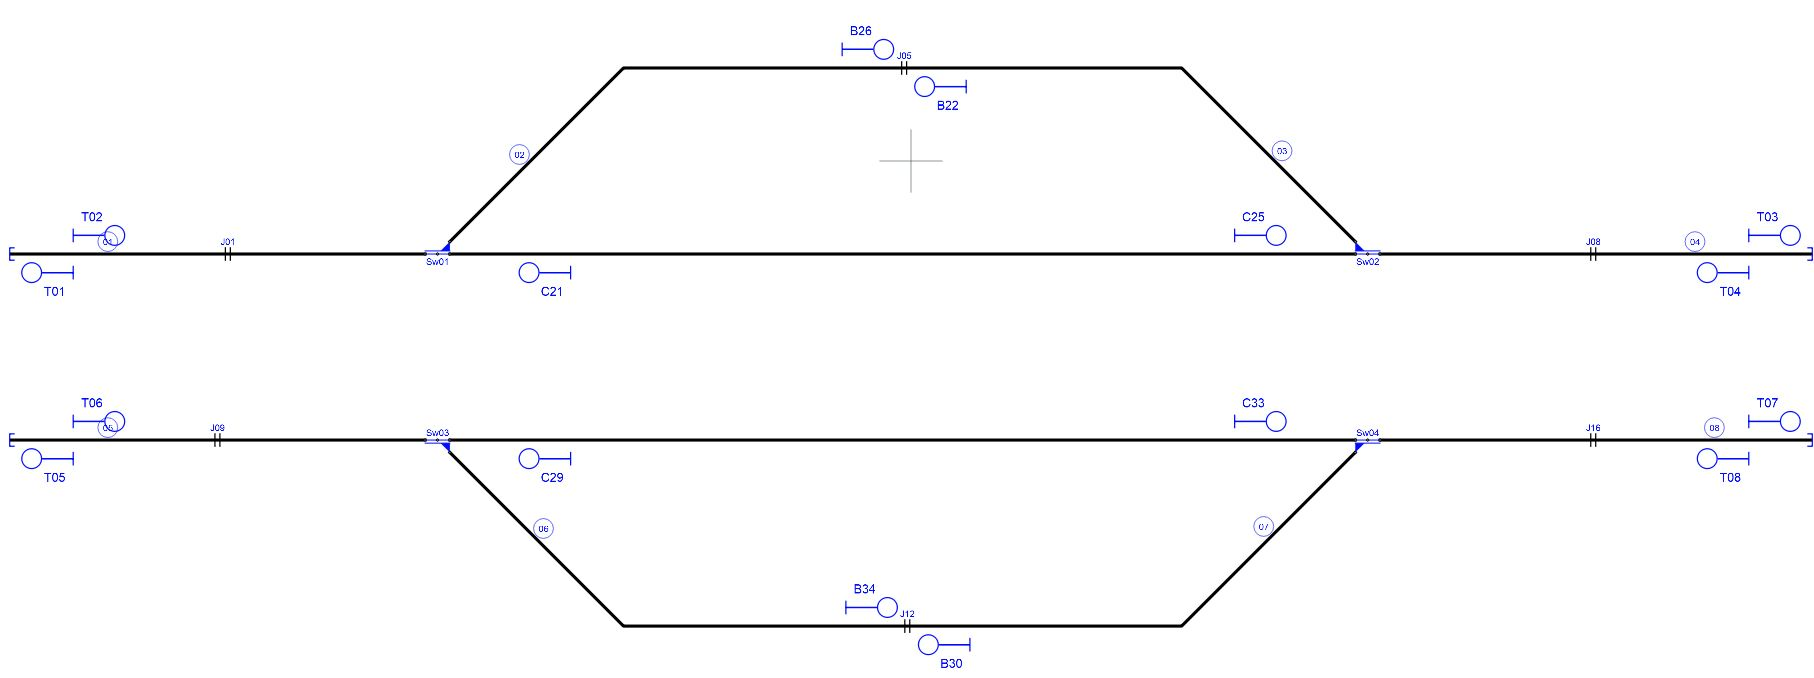
\includegraphics[width=1\textwidth]{resultados-obtenidos/ejemplo5/images/5_RNA.png}
		\centering\caption{Señalamiento generado y simplificado por el RNA.}
		\label{fig:EJ5_7}
	\end{figure}
	
	Al finalizar la generación del señalamiento, el RNA debe detectar todas las posibles rutas admitidas por la red para crear la tabla de enclavamientos. El RNA exporta los resultados del análisis en los siguientes cuatro documentos: Infrastructure.RNA (Apéndice \ref{sec:infrastructureRNA}), SafePoint.RNA (Apéndice \ref{sec:safePointsRNA}), Signalling.RNA (Apéndice \ref{sec:signallingRNA}) y Routes.RNA (Apéndice \ref{sec:routesRNA}).	
    \subsection{Red de grafos generada por el RNA}

	La información exportada en el Código \ref{lst:EJ5_5}, Código \ref{lst:EJ5_6} y Código \ref{lst:EJ5_7} es utilizada resumida por el RNA para una mejor interpretación. El resultado de este resumen se ilustra en el diagrama de la Figura \ref{fig:EJ5_8}.
	
	\begin{figure}[H]
		\centering
		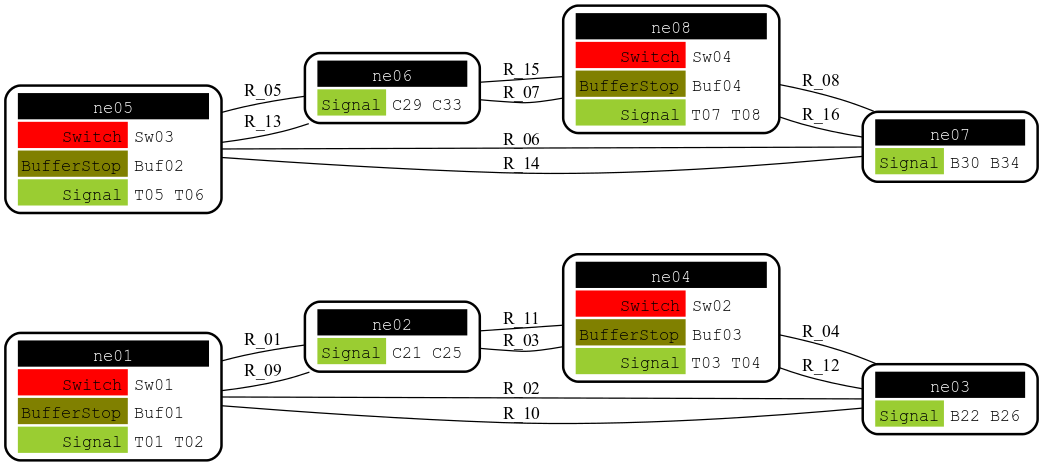
\includegraphics[width=1\textwidth]{Figuras/Graph_5}
		\centering\caption{Red de grafos generada por el RNA para el ejemplo 5.}
		\label{fig:EJ5_8}
	\end{figure}
	
	Cada nodo del grafo de la Figura \ref{fig:EJ5_8} corresponde a un \textit{netElement}. En cada nodo se listan todos los elementos ferroviarios contenidos por en \textit{netElement}. Las aristas del grafo son las rutas que los conectan. De esta manera, es posible detectar visualmente que los grafos que definen ambas vías principales son disconexos, compatibles con lo esperado en base a la Figura \ref{fig:EJ5_1}.
    \subsection{Señalamiento generado por el RNA}

    El RNA también exporta la misma información mostrada en el Código \ref{lst:EJ5_8} en una hoja de cálculo, similar a la que se visualiza en la Tabla \ref{Tab:tabla_generated_5}.
    
    \begin{table}[!h]
        {
        \caption{Tabla de enclavamiento del ejemplo 5 generada por el RNA.}
        \label{Tab:tabla_generated_5}
        \centering
        \resizebox{1\textwidth}{!}{
            \begin{tabular}{ c c c c c c c }
                \hline	
                    Ruta & Inicio & Final & Cambio & Plataforma & Cruce & netElement \\	
                \hline
                    R$_{01}$  & T$_{02}$ & C$_{25}$ & Sw$_{01}^{N}$ & - & - & ne$_{01}$-ne$_{03}$\\
                    R$_{02}$  & T$_{02}$ & B$_{26}$ & Sw$_{01}^{R}$ & - & - & ne$_{01}$-ne$_{04}$\\
                    R$_{03}$  & T$_{04}$ & C$_{21}$ & Sw$_{02}^{N}$ & - & - & ne$_{04}$-ne$_{03}$\\
                    R$_{04}$  & T$_{04}$ & B$_{26}$ & Sw$_{02}^{R}$ & - & - & ne$_{04}$-ne$_{04}$\\
                    R$_{05}$  & T$_{06}$ & C$_{33}$ & Sw$_{03}^{N}$ & - & - & ne$_{05}$-ne$_{06}$\\
                    R$_{06}$  & T$_{06}$ & B$_{34}$ & Sw$_{03}^{R}$ & - & - & ne$_{05}$-ne$_{07}$\\
                    R$_{07}$  & T$_{08}$ & C$_{29}$ & Sw$_{04}^{N}$ & - & - & ne$_{08}$-ne$_{06}$\\
                    R$_{08}$  & T$_{08}$ & B$_{30}$ & Sw$_{04}^{R}$ & - & - & ne$_{08}$-ne$_{07}$\\
                    R$_{09}$  & C$_{21}$ & T$_{01}$ & Sw$_{01}^{N}$ & - & - & ne$_{02}$-ne$_{01}$\\
                    R$_{10}$  & B$_{22}$ & T$_{01}$ & Sw$_{01}^{R}$ & - & - & ne$_{03}$-ne$_{01}$\\
                    R$_{11}$  & C$_{25}$ & T$_{03}$ & Sw$_{02}^{N}$ & - & - & ne$_{02}$-ne$_{04}$\\
                    R$_{12}$  & B$_{26}$ & T$_{03}$ & Sw$_{02}^{R}$ & - & - & ne$_{03}$-ne$_{04}$\\
                    R$_{13}$  & C$_{29}$ & T$_{05}$ & Sw$_{03}^{N}$ & - & - & ne$_{06}$-ne$_{05}$\\
                    R$_{14}$  & B$_{30}$ & T$_{05}$ & Sw$_{03}^{R}$ & - & - & ne$_{07}$-ne$_{05}$\\
                    R$_{15}$  & C$_{33}$ & T$_{07}$ & Sw$_{04}^{N}$ & - & - & ne$_{06}$-ne$_{08}$\\
                    R$_{16}$  & B$_{34}$ & T$_{07}$ & Sw$_{04}^{R}$ & - & - & ne$_{07}$-ne$_{08}$\\
                \hline
            \end{tabular}
        }
     }
    \end{table}
    
    En una primera inspección podemos ver que el nuevo señalamiento tiene 16 rutas, al igual que el señalamiento original que también posee 16 rutas. Esto se debe a que el señalamiento original ya contemplaba todas las rutas posibles y el RNA generó un nuevo señalamiento equivalente, sin eliminar rutas ni tampoco agregando rutas que no sean útiles.
    \section{Validación del sistema}

    La validación de las rutas de la tabla de enclavamientos es realizada por el RNA aplicando el Algoritmo \ref{alg:interlocking_tables}, explicado en la Sección \ref{sec:validar_tabla}. Las 16 rutas del señalamiento original (Tabla \ref{Tab:tabla_original_5}) tienen 16 rutas equivalentes en el señalamiento generado por el RNA (Tabla \ref{Tab:tabla_generated_5}), tal como se puede visualizar en la Tabla \ref{Tab:tabla_validation_5}, generada automáticamente por el RNA.

    \begin{table}[!h]
        {
        \caption{Equivalencias entre las rutas originales y las generadas por el RNA.}
        \label{Tab:tabla_validation_5}
        \centering
        \resizebox{0.9\textwidth}{!}{
            \begin{tabular}{ c c c c }
                \hline	
                    Original & Señales & RNA & Señales \\	
                \hline
                    R$_{01}$ & S$_{01}$-S$_{06}$ & R$_{01}$ & T$_{02}$-C$_{25}$ \\
                    R$_{02}$ & S$_{05}$-S$_{13}$ & R$_{09}$ & C$_{21}$-T$_{01}$ \\
                    R$_{03}$ & S$_{01}$-S$_{03}$ & R$_{02}$ & T$_{02}$-B$_{26}$ \\
                    R$_{04}$ & S$_{04}$-S$_{13}$ & R$_{10}$ & B$_{22}$-T$_{01}$ \\
                    R$_{05}$ & S$_{02}$-S$_{04}$ & R$_{03}$ & T$_{04}$-C$_{21}$ \\
                    R$_{06}$ & S$_{06}$-S$_{15}$ & R$_{11}$ & C$_{25}$-T$_{03}$ \\
                    R$_{07}$ & S$_{02}$-S$_{05}$ & R$_{04}$ & T$_{04}$-B$_{26}$ \\
                    R$_{08}$ & S$_{03}$-S$_{15}$ & R$_{12}$ & B$_{26}$-T$_{03}$ \\
                    R$_{09}$ & S$_{07}$-S$_{11}$ & R$_{05}$ & T$_{06}$-C$_{33}$ \\
                    R$_{10}$ & S$_{10}$-S$_{14}$ & R$_{13}$ & C$_{29}$-T$_{05}$ \\
                    R$_{11}$ & S$_{07}$-S$_{09}$ & R$_{06}$ & T$_{06}$-B$_{34}$ \\
                    R$_{12}$ & S$_{08}$-S$_{14}$ & R$_{14}$ & B$_{30}$-T$_{05}$ \\
                    R$_{13}$ & S$_{12}$-S$_{10}$ & R$_{07}$ & T$_{08}$-C$_{29}$ \\
                    R$_{14}$ & S$_{11}$-S$_{16}$ & R$_{15}$ & C$_{33}$-T$_{07}$ \\
                    R$_{15}$ & S$_{12}$-S$_{08}$ & R$_{08}$ & T$_{08}$-B$_{30}$ \\
                    R$_{16}$ & S$_{09}$-S$_{16}$ & R$_{16}$ & B$_{34}$-T$_{07}$ \\
                \hline
            \end{tabular}
     		}
        }    
    \end{table}
    
    Todas las rutas generadas por el RNA (Tabla \ref{Tab:tabla_generated_5}) tienen una ruta equivalente en el señalamiento original (Tabla \ref{Tab:tabla_original_5}). El RNA no ha generado nuevas señales ni rutas ya que el señalamiento original ya satisfacía todos los requerimientos de seguridad necesarios. Tampoco se eliminaron señales ni rutas, lo que demuestra que el RNA puede mejorar los sistemas de enclavamientos cuando es posible, o igualarlos cuando se ha alcanzado la cota máxima de seguridad, sin recurrir a redundancias improductivas.
    
    Para finalizar, el RNA comprueba los principios de señalamiento ferroviario explicados en la Sección \label{sec:validar_principios}, aplicando los algoritmos indicados, de los cuáles se obtuvieron los siguientes resultados:
    
    \begin{itemize}
    	\item Principio de autoridad (Algoritmo \ref{alg:ppio_autoridad}): cobertura del 100\% de los \textit{netElements}.
    	\item Principio de claridad (Algoritmo \ref{alg:ppio_claridad}): rutas 100\% independientes.
    	\item Principio de anticipación (Algoritmo \ref{alg:ppio_anticipacion}): cobertura del 100\% de los puntos críticos.
    	\item Principio de granularidad (Algoritmo \ref{alg:ppio_granularidad}): 100\% de rutas divididas a su mínima expresión.
    	\item Principio de terminalidad (Algoritmo \ref{alg:ppio_terminalidad}): 100\% de finales de vías protegidos.
    	\item Principio de infraestructura (Algoritmo \ref{alg:ppio_infraestructura}): 100\% de infraestructura protegida.
    	\item Principio de no bloqueo (Algoritmo \ref{alg:ppio_nobloqueo}): 100\% de cambios de vías protegidos.
    \end{itemize}	
    \section{Sistema generado por el ACG}

	En base a la red de grafos, ilustrada en la Figura \ref{fig:EJ5_8}, el ACG determinó la siguiente cantidad de elementos, tal puede visualizarse en el Código \ref{lst:EJ5_8}.
	
	\begin{lstlisting}[language = {}, caption = Cantidad de elementos a implementar por el ACG, label = {lst:EJ5_8}]
	n_netElements:8
	n_switch:4
	n_doubleSwitch:0
	n_borders:0
	n_buffers:4
	n_levelCrossings:0
	n_platforms:0
	n_scissorCrossings:0
	n_signals:16
	N : 44
	\end{lstlisting}
	
	Se repetirán los pasos detallados en el ejemplo 1, Sección \ref{sec:EJEMPLO1_ACG}, por lo que solamente se destacarán aspectos particulares de este ejemplo. El ACG genera 62 archivos en formato VHDL. El archivo \textit{Arty\_Z7-10.XDC} es el mismo para todos los ejemplos, al ser invariante respecto a la cantidad de pines a utilizar. Se deberá modificar el script mostrado en el Código \ref{lst:EJ1_script} y cambiar el parámetro \textit{chosen} a 5 para automatizar la importación de los archivos del ejemplo 5 y desvincular cualquier otro conjunto de archivos de ejemplos anteriores.
	
	Una vez ejecutado el script, Vivado ordenará los archivos de forma jerárquica, donde el módulo \textit{global} incluye todos los módulos que fueron detallados en la Sección \ref{sec:interlockingArch}. Cada una de las instancias del módulo \textit{network} contienen sus propias 44 instancias de los mismos módulos de cada elemento ferroviario ya que N, cantidad de elementos ferroviarios, es 44 en el Código \ref{lst:EJ5_8}. El ejemplo 5 utiliza mas de 13800 sub módulos conectados automáticamente mediante mas de 27000 señales, lo cual se aleja bastante de un desarrollo que pueda realizarse manualmente de forma trivial.
	
	Cuando Vivado genera el diagrama de bloques ya tenemos la certeza de que el código VHDL ha pasado la prueba de sintaxis del entorno de desarrollo. A continuación, se deberá sintetizar e implementar el sistema para generar el bitstream que será utilizado para programar la FPGA. Los procesos de síntesis e implementación fueron detallados en el ejemplo 1, Sección \ref{sec:EJEMPLO1_ACG}.
	
	Los resultados de ambos procesos son detallados en la Tabla \ref{Tab:tabla_ACG_5}. Los porcentajes de uso son calculados por Vivado automáticamente, teniendo en cuenta que la plataforma Arty Z7 20 posee 53200 Look-Up-Tables (LUTs), 106400 Flip-Flops (FFs), 125 Pines de entrada y salida (IOs) y 32 Buffers (BUFGs), tal cómo se explicó en la Sección \ref{sec:AGG}. En este ejemplo, la cantidad de recursos utilizados es baja y el tiempo de síntesis e implementación es de 41 y 57 segundos, respectivamente.
		
	\begin{table}[H]
		{
			\caption{Síntesis e implementación del ejemplo 5 generado por el ACG.}
			\label{Tab:tabla_ACG_5}
			\centering
			%\small
			%\centering
			\begin{center}
				\resizebox{0.7\textwidth}{!}{
					\begin{tabular}{ c c c c }
						\hline	
						Recursos & Síntesis & Implementación & Uso \\	
						\hline
						LUT & 2328 & 2307 & 4.38-4.34\%\\
						FF & 2344 & 2347 & 2.20-2.21\%\\
						IO & 15 & 15 & 12.00\%\\
						BUFG & 3 & 3 & 9.38\%\\
						\hline
					\end{tabular}
				}
			\end{center}
		}    
	\end{table}
   
	%\section{Ejemplo 6}
    
    \section{Topología ferroviaria original}

	El sexto ejemplo, ilustrado en la Figura \ref{fig:EJ6_1}, es una topología diseñada por el autor de esta tesis, en base a una línea principal con tres niveles de ramificaciones y curvas dentro de un mismo \textit{netElement}. Las primeras ramificaciones, utilizando los cambio de vías Sw01, Sw02 o Sw05, es una ramificación simple. La segunda ramificación, utilizando el cambio de vías Sw03, es una ramificación compleja al incluir el cambio de vías Sw01 previamente. Ademas, los \textit{netElements} ne4, ne7, ne10 y ne41 presentan curvas que incrementan la dificultad del diseño del señalamiento. El objetivo de este ejemplo fue comprobar el funcionamiento del RNA con una topología de múltiples ramificaciones anidadas combinadas con curvas. Para mas detalles de este ejemplo, incluyendo las figuras, tablas y explicaciones paso a paso, consultar el repositorio de GitHub \cite{GITHUB_PHD}.
	
	\begin{figure}[h]
		\centering
		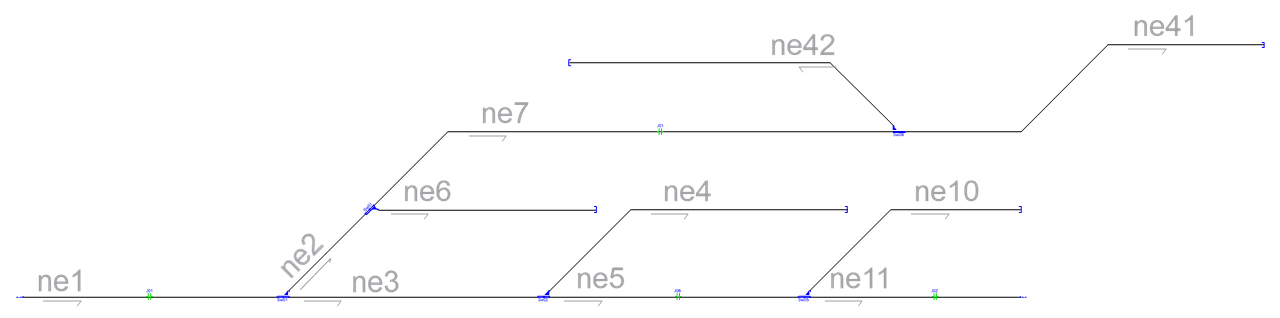
\includegraphics[width=1\textwidth]{resultados-obtenidos/ejemplo6/images/6_empty.png}
		\centering\caption{Topología ferroviaria del ejemplo 6 sin señalamiento.}
		\label{fig:EJ6_1}
	\end{figure}
	
	Para incrementar la dificultad del análisis y obtener resultados mas completos, se incluyeron finales de vías relativos y absolutos. No se incluyeron plataformas o cruces de vías.

    \section{Señalamiento original}

    El señalamiento original, ilustrado en la Figura \ref{fig:EJ6_2}, incluye señales de parada próximas a los finales de vías absolutos (S11, S12, S13, S14, S16), señales de maniobras antes de converger en una vía principal (S10, S15, S20) y señales múltiples para cambios de vías divergentes (S01, S06, S07, S21), entre varias otras señales.
    
    \begin{figure}[H]
    	\centering
    	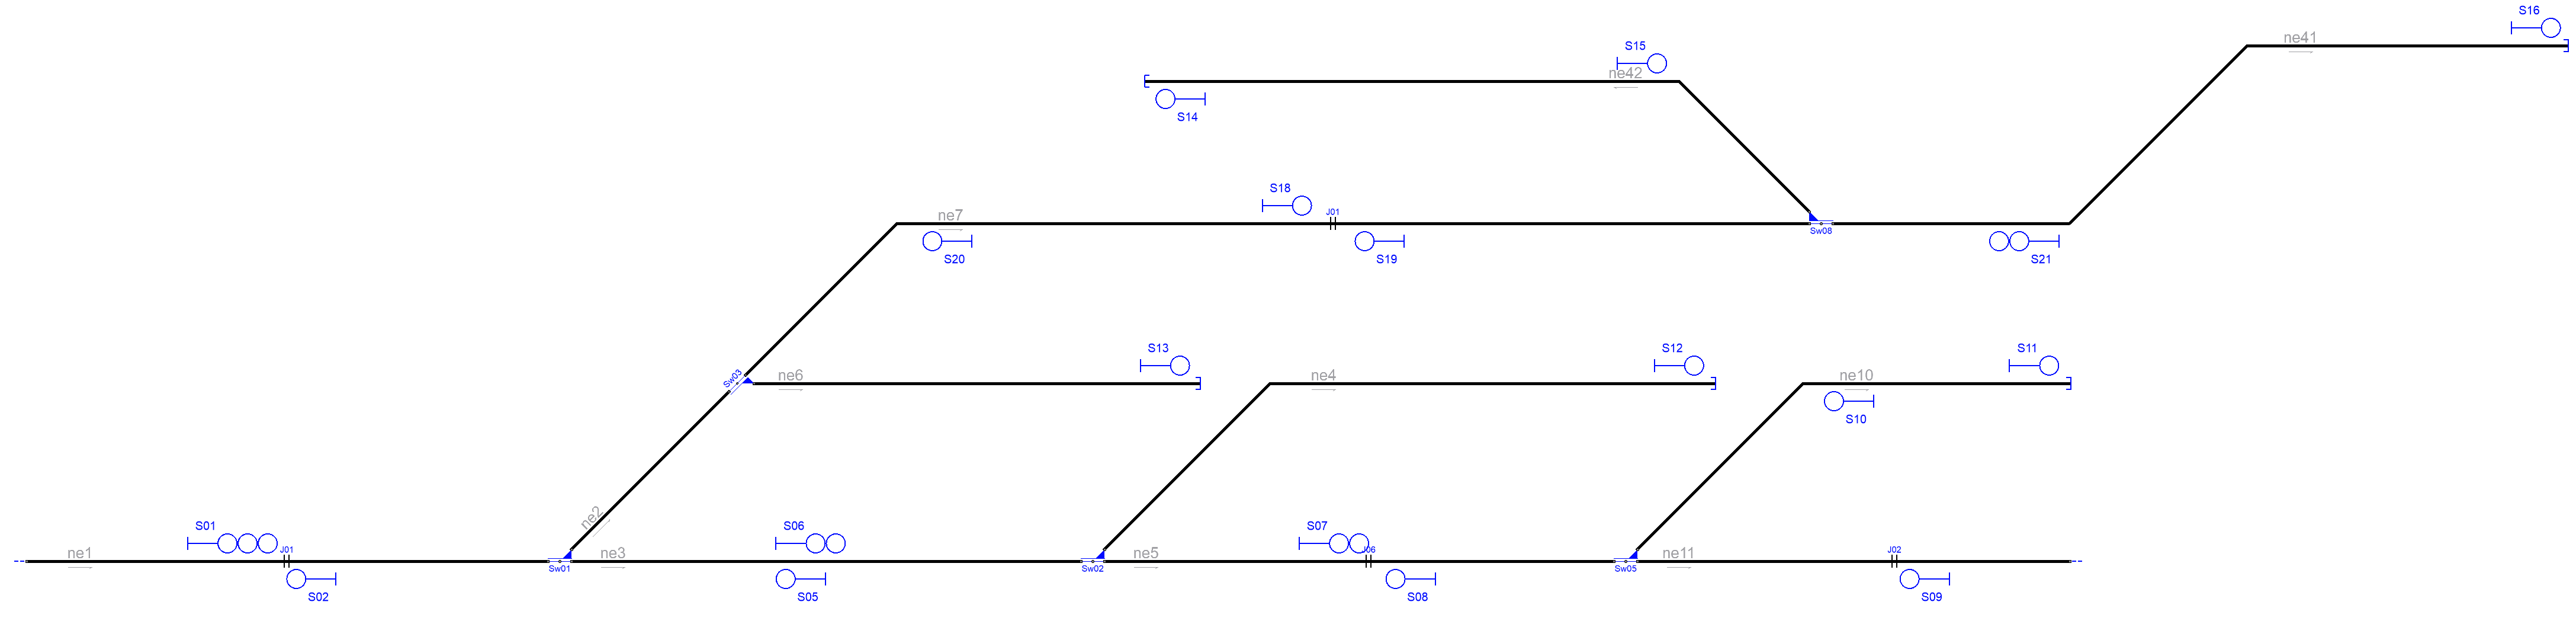
\includegraphics[width=1\textwidth]{resultados-obtenidos/ejemplo6/images/6_original.png}
    	\centering\caption{Señalamiento original del ejemplo 6.}
    	\label{fig:EJ6_2}
    \end{figure}
    
    Estas señales permiten definir hasta un máximo de 16 rutas, todas ellas detalladas en la Tabla \ref{Tab:tabla_original_6}. En una primera inspección, se puede comprobar que todos los elementos ferroviarios son alcanzados por al menos una de las rutas, en al menos una dirección. Además, todos los cambios de vías son utilizados, de forma simple o compuesta. 
    
    \begin{table}[H]
        {
        \caption{Tabla de enclavamiento original del ejemplo 6.}
        \label{Tab:tabla_original_6}
        \centering
        \resizebox{1\textwidth}{!}{
            \begin{tabular}{ c c c c c c c }
                \hline	
                    Ruta & Inicio & Final & Cambio & Plataforma & Cruce & netElement \\	
                \hline
                    R$_{01}$  & S$_{01}$ & S$_{06}$ & Sw$_{01}^{N}$ & - & - & ne$_{01}$-ne$_{03}$\\
                    R$_{02}$  & S$_{01}$ & S$_{13}$ & Sw$_{01}^{R}$+Sw$_{03}^{R}$ & - & - & ne$_{01}$-ne$_{06}$\\
                    R$_{03}$  & S$_{01}$ & S$_{18}$ & Sw$_{01}^{R}$+Sw$_{03}^{R}$ & - & - & ne$_{01}$-ne$_{07}$\\
                    R$_{04}$  & S$_{06}$ & S$_{07}$ & Sw$_{02}^{N}$ & - & - & ne$_{03}$-ne$_{05}$\\
                    R$_{05}$  & S$_{06}$ & S$_{12}$ & Sw$_{02}^{R}$ & - & - & ne$_{03}$-ne$_{04}$\\
                    R$_{06}$  & S$_{21}$ & S$_{19}$ & Sw$_{08}^{N}$ & - & - & ne$_{41}$-ne$_{07}$\\
                    R$_{07}$  & S$_{21}$ & S$_{14}$ & Sw$_{08}^{R}$ & - & - & ne$_{41}$-ne$_{42}$\\
                    R$_{08}$  & S$_{05}$ & S$_{02}$ & Sw$_{01}^{N}$ & - & - & ne$_{03}$-ne$_{01}$\\
                    R$_{09}$  & S$_{09}$ & S$_{08}$ & Sw$_{05}^{N}$ & - & - & ne$_{11}$-ne$_{05}$\\
                    R$_{10}$  & S$_{08}$ & S$_{05}$ & Sw$_{02}^{N}$ & - & - & ne$_{05}$-ne$_{03}$\\
                    R$_{11}$  & S$_{10}$ & S$_{08}$ & Sw$_{05}^{R}$ & - & - & ne$_{10}$-ne$_{05}$\\
                    R$_{12}$  & S$_{15}$ & S$_{16}$ & Sw$_{08}^{R}$ & - & - & ne$_{42}$-ne$_{41}$\\
                    R$_{13}$  & S$_{18}$ & S$_{16}$ & Sw$_{08}^{N}$ & - & - & ne$_{07}$-ne$_{41}$\\
                    R$_{14}$  & S$_{19}$ & S$_{20}$ & - & - & - & ne$_{07}$\\
                    R$_{15}$  & S$_{20}$ & S$_{02}$ & Sw$_{01}^{R}$+Sw$_{03}^{N}$ & - & - & ne$_{07}$-ne$_{01}$\\
                    R$_{16}$  & S$_{07}$ & S$_{11}$ & Sw$_{05}^{R}$ & - & - & ne$_{05}$-ne$_{10}$\\
                \hline
            \end{tabular}
        }
     }
    \end{table}
    
    Algunas rutas abarcan mas de un \textit{netElement}, como por ejemplo la ruta R15 que comienza en la señal S20 y finaliza en la señal S02, atravesando los \textit{netElements} ne07 y ne01, utilizando los cambios de vías Sw01 y Sw03, en posición reversa y normal respectivamente.
    \subsection{Generación de señalamiento paso a paso}

\lipsum[1]

\begin{figure}[H]
	\centering
	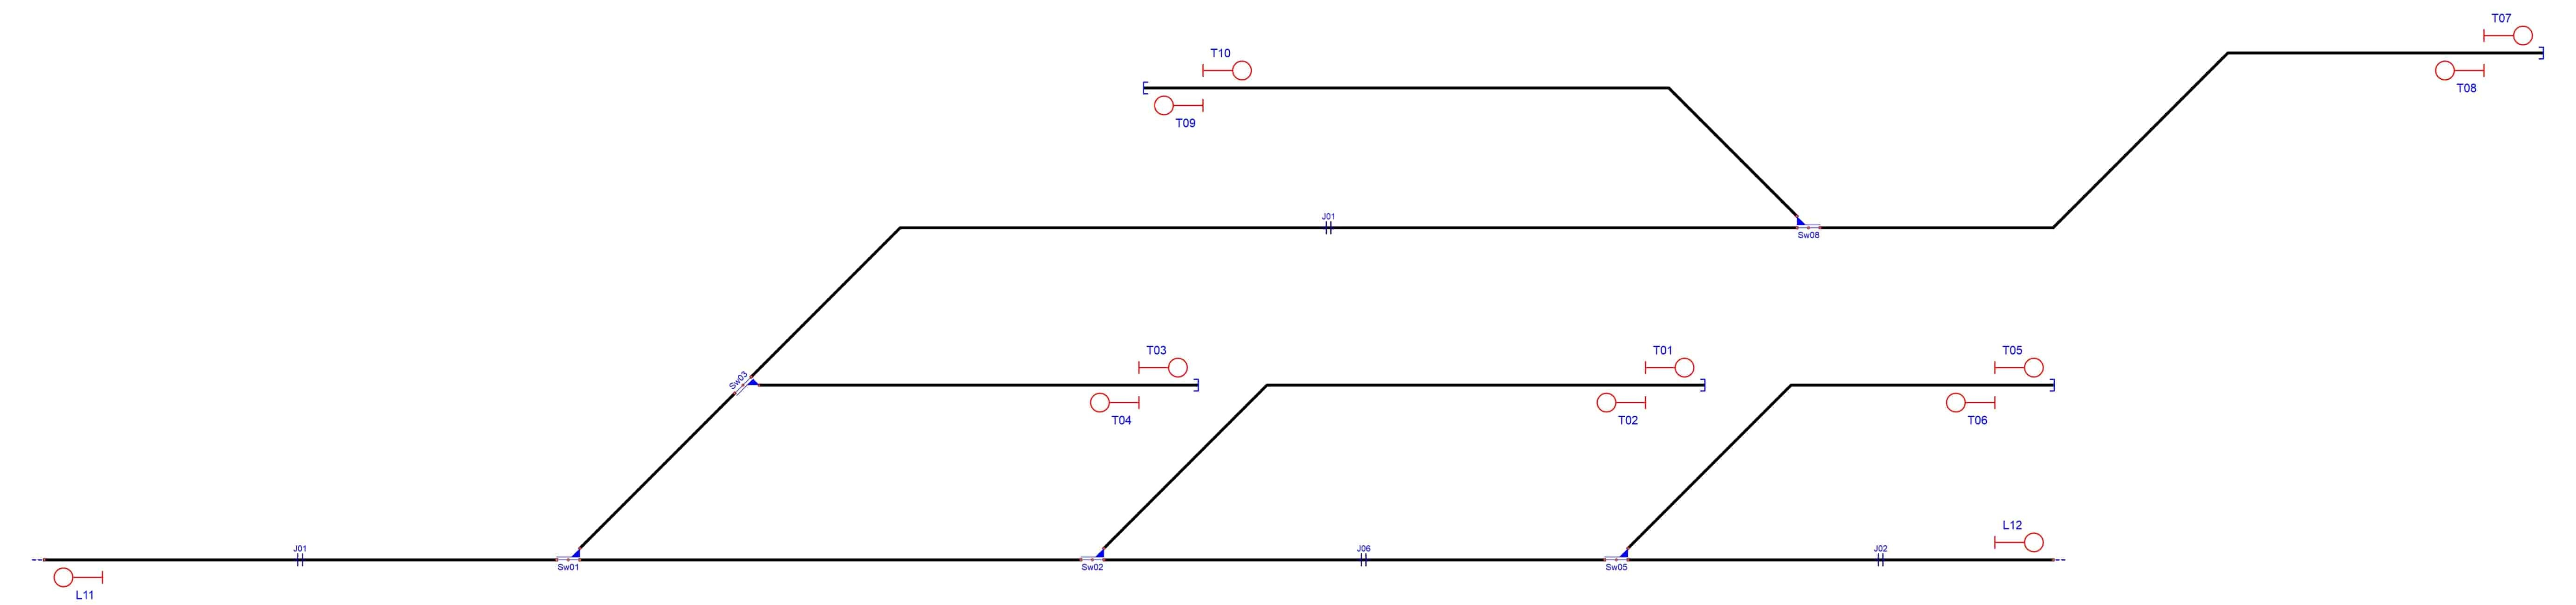
\includegraphics[width=1\textwidth]{resultados-obtenidos/ejemplo6/images/6_step1.png}
	\centering\caption{Señalamiento generado por el RNA para proteger el fín de vía.}
	%\label{fig:LC_P2}
\end{figure}

\lipsum[1]

\begin{figure}[H]
	\centering
	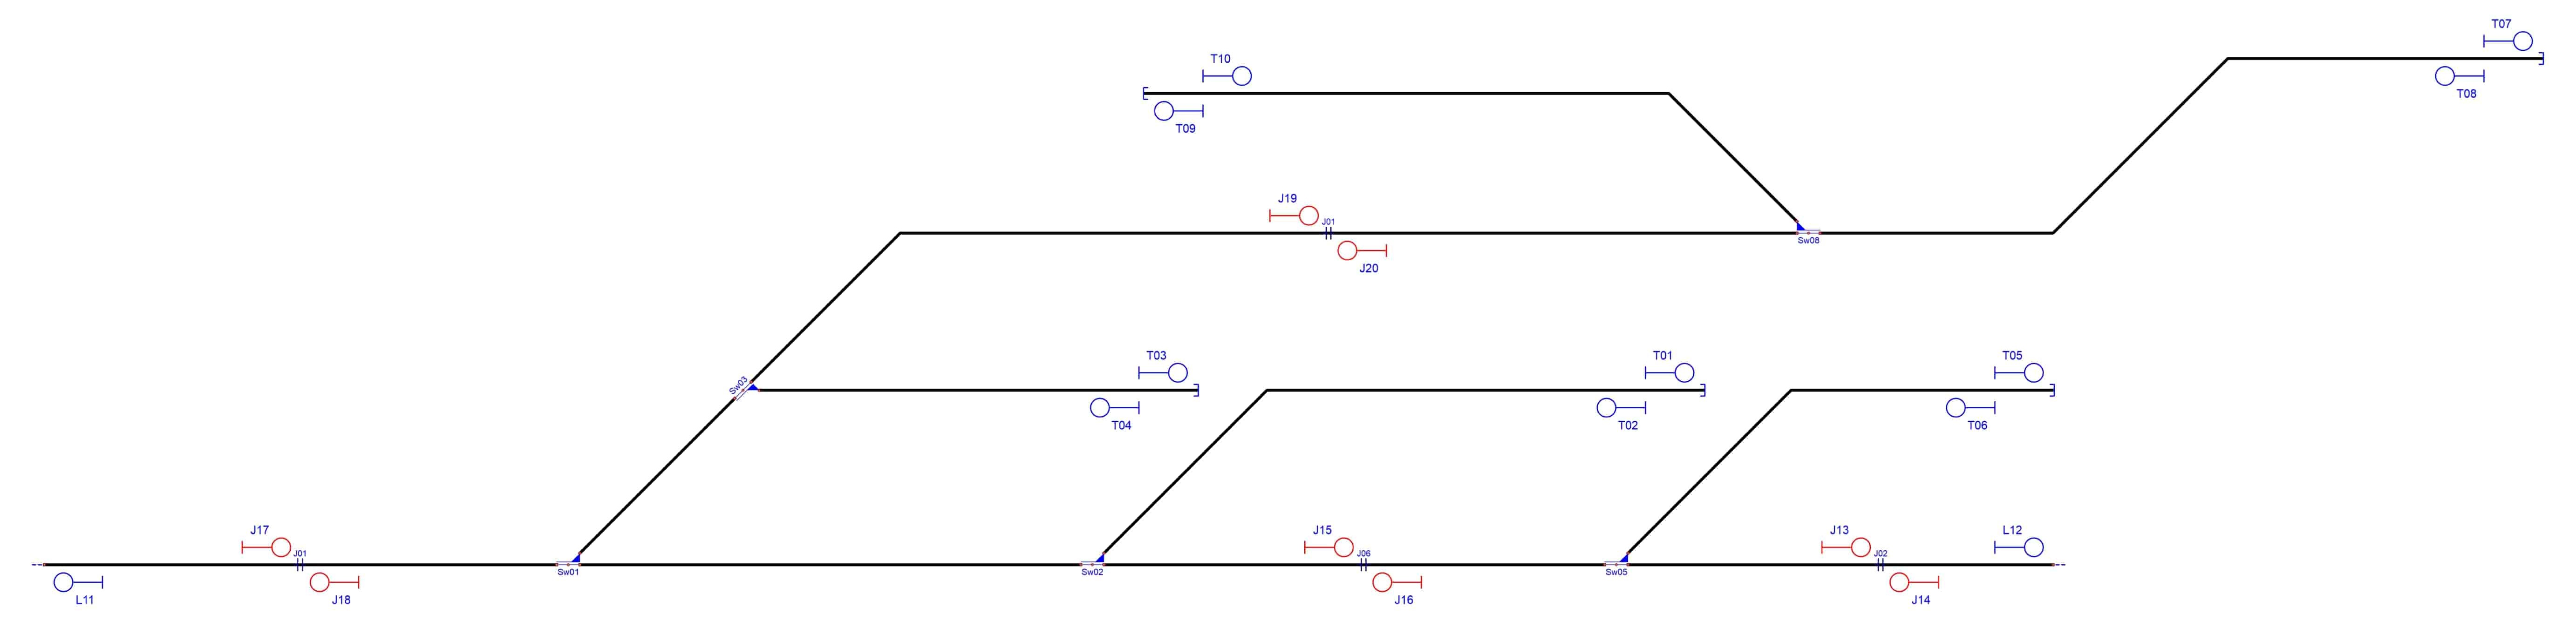
\includegraphics[width=1\textwidth]{resultados-obtenidos/ejemplo6/images/6_step2.png}
	\centering\caption{Señalamiento generado por el RNA para proteger las junturas.}
	%\label{fig:LC_P2}
\end{figure}

\lipsum[1]

\begin{figure}[H]
	\centering
	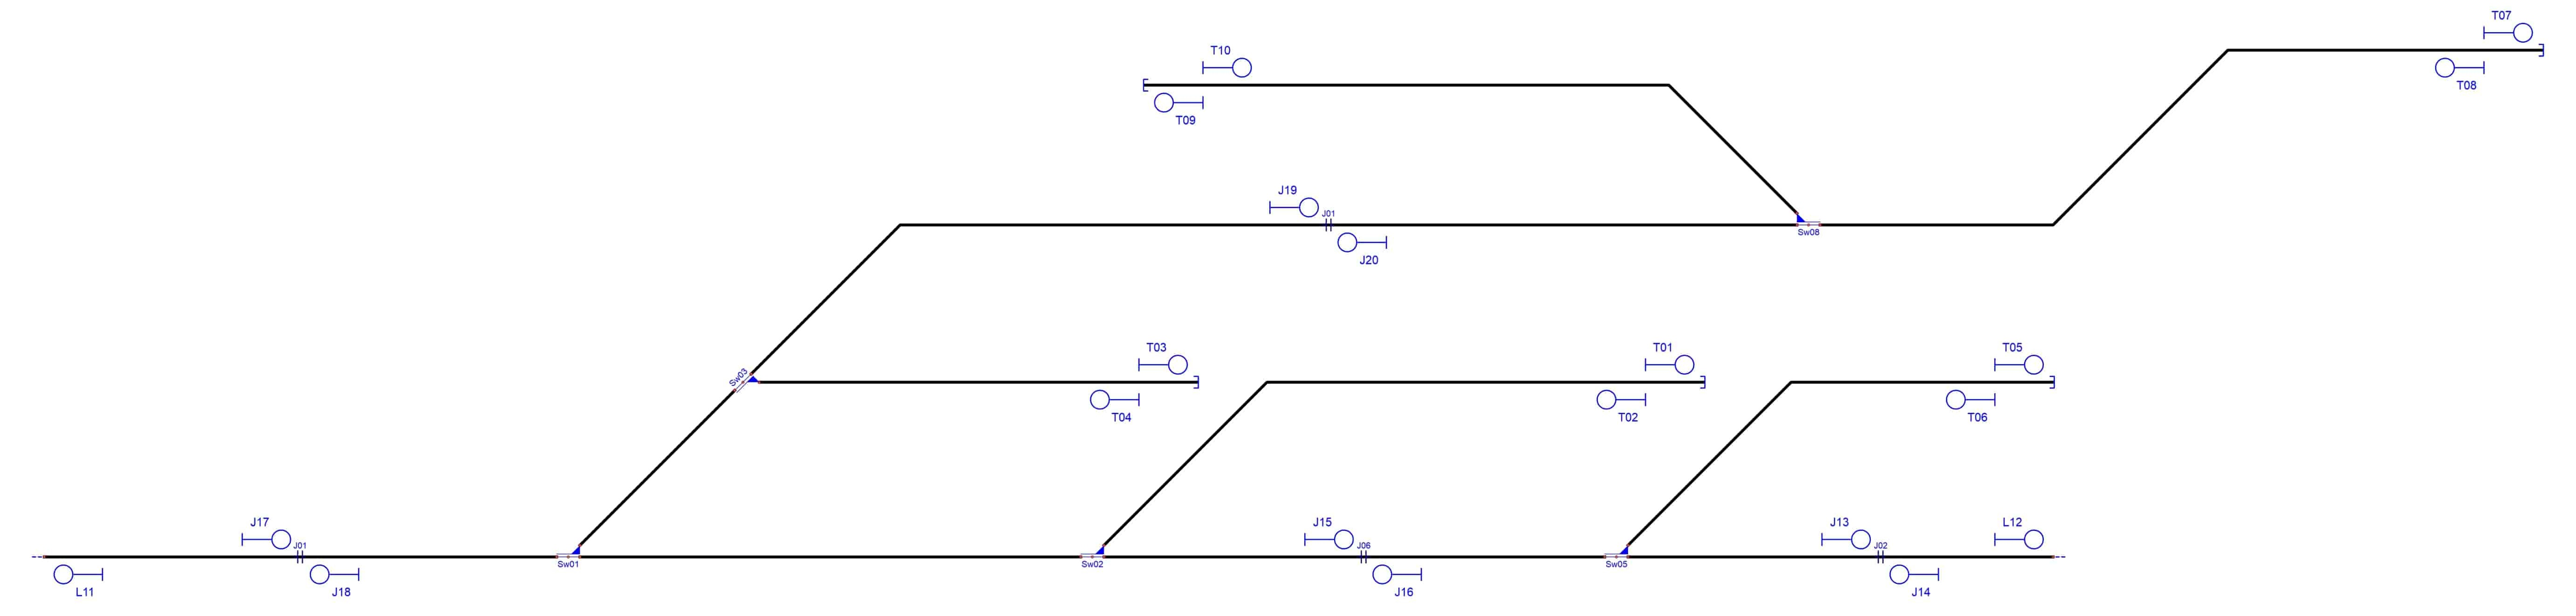
\includegraphics[width=1\textwidth]{resultados-obtenidos/ejemplo6/images/6_step3.png}
	\centering\caption{Señalamiento generado por el RNA para proteger plataformas y cruces de vía.}
	%\label{fig:LC_P2}
\end{figure}

\lipsum[1]

 \begin{figure}[H]
	\centering
	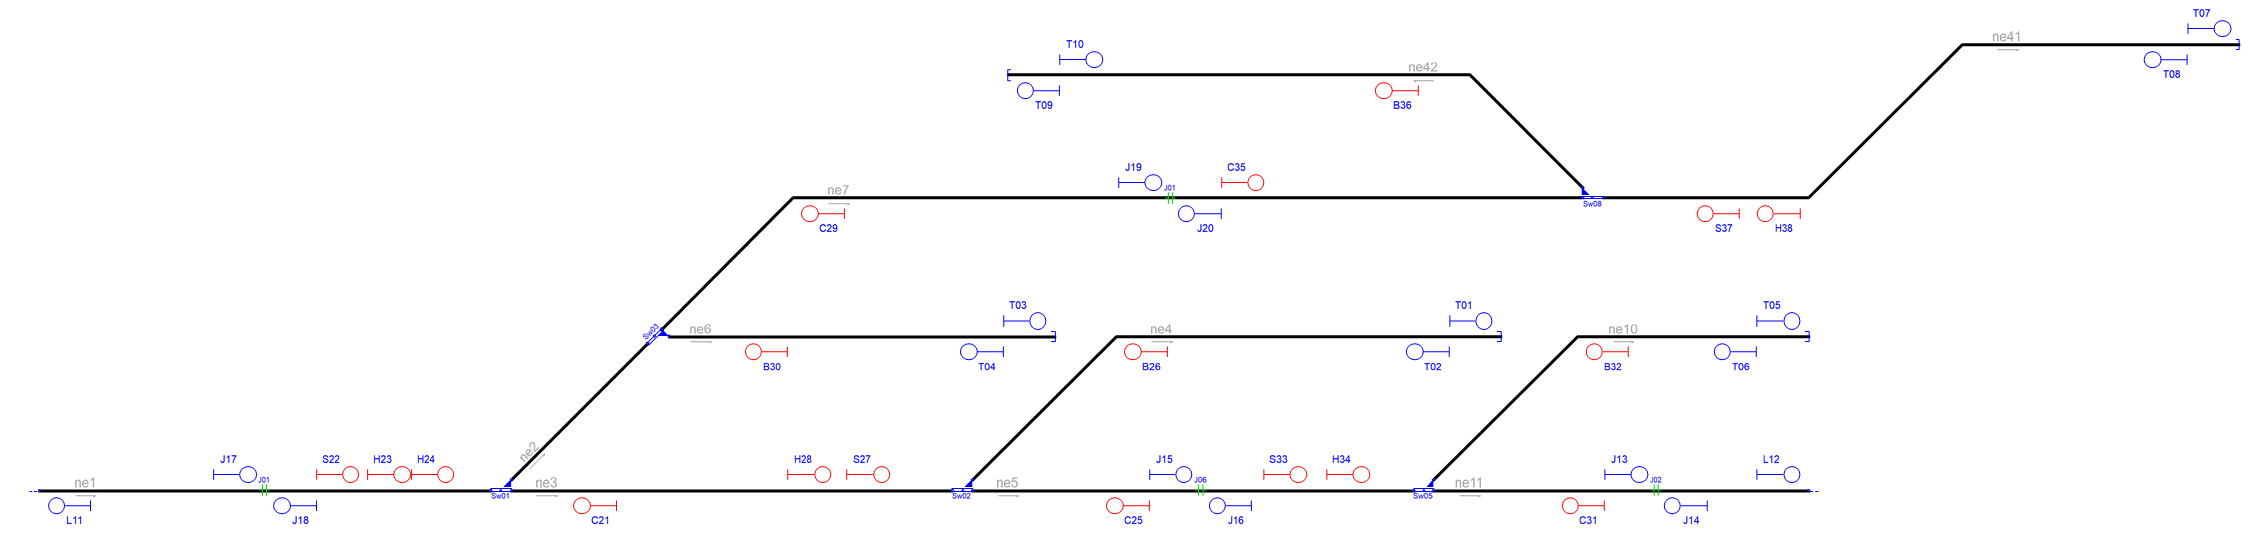
\includegraphics[width=1\textwidth]{resultados-obtenidos/ejemplo6/images/6_step4.png}
	\centering\caption{Señalamiento generado por el RNA para proteger las máquinas de cambios.}
	%\label{fig:LC_P2}
\end{figure}

\lipsum[1]

 \begin{figure}[H]
	\centering
	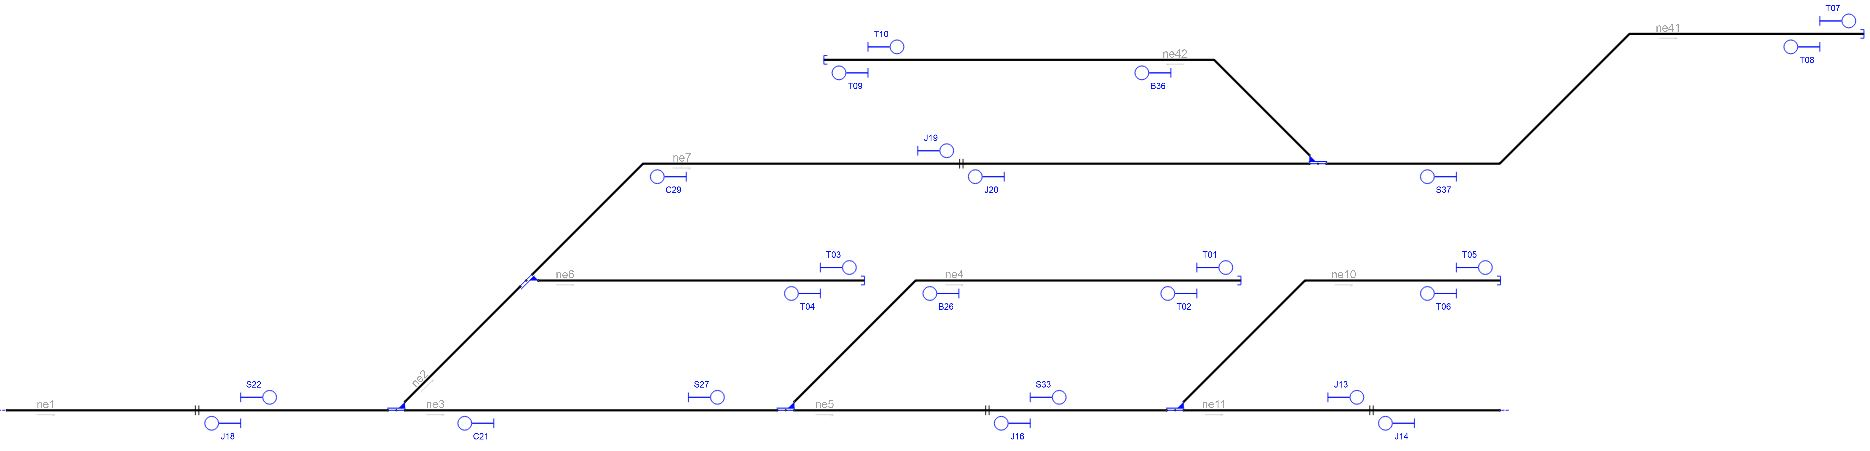
\includegraphics[width=1\textwidth]{resultados-obtenidos/ejemplo6/images/6_RNA.png}
	\centering\caption{Señalamiento generado y simplificado por el RNA.}
	%\label{fig:LC_P2}
\end{figure}

\lipsum[1]
    \section{Señalamiento generado por el RNA}

    El RNA también exporta la información mostrada en el Código \ref{lst:EJ6_8} en una hoja de cálculo, similar a la que se visualiza en la Tabla \ref{Tab:tabla_generated_6}.
    
    \begin{table}[H]
        {
        \caption{Tabla de enclavamiento del ejemplo 6 generada por el RNA.}
        \label{Tab:tabla_generated_6}
        %\centering
        \begin{center}      
        	\resizebox{0.8\textwidth}{!}{
            \begin{tabular}{ c c c c c c c }
                \hline	
                    Ruta & Inicio & Final & Cambio & Plataforma & Cruce & netElement \\	
                \hline
                    R$_{01}$  & T$_{02}$ & B$_{26}$ & - & - & - & ne$_{04}$\\
                    R$_{02}$  & T$_{04}$ & J$_{18}$ & Sw$_{01}^{R}$+Sw$_{03}^{R}$ & - & - & ne$_{06}$-ne$_{01}$\\
                    R$_{03}$  & T$_{06}$ & J$_{16}$ & Sw$_{05}^{R}$ & - & - & ne$_{10}$-ne$_{05}$\\
                    R$_{04}$  & T$_{08}$ & S$_{37}$ & - & - & - & ne$_{41}$\\
                    R$_{05}$  & T$_{10}$ & T$_{07}$ & Sw$_{08}^{R}$ & - & - & ne$_{42}$-ne$_{41}$\\
                    R$_{06}$  & J$_{14}$ & J$_{16}$ & Sw$_{05}^{N}$ & - & - & ne$_{11}$-ne$_{05}$\\
                    R$_{07}$  & J$_{16}$ & C$_{21}$ & Sw$_{02}^{N}$ & - & - & ne$_{05}$-ne$_{03}$\\
                    R$_{08}$  & J$_{19}$ & T$_{07}$ & Sw$_{08}^{N}$ & - & - & ne$_{07}$-ne$_{41}$\\
                    R$_{09}$  & J$_{20}$ & C$_{29}$ & - & - & - & ne$_{07}$\\
                    R$_{10}$  & C$_{21}$ & J$_{18}$ & Sw$_{01}^{N}$ & - & - & ne$_{03}$-ne$_{01}$\\
                    R$_{11}$  & S$_{22}$ & S$_{27}$ & Sw$_{01}^{N}$ & - & - & ne$_{01}$-ne$_{03}$\\
                    R$_{12}$  & S$_{22}$ & J$_{19}$ & Sw$_{01}^{R}$+Sw$_{03}^{N}$ & - & - & ne$_{01}$-ne$_{07}$\\
                    R$_{13}$  & S$_{22}$ & T$_{03}$ & Sw$_{01}^{R}$+Sw$_{03}^{R}$ & - & - & ne$_{01}$-ne$_{06}$\\
                    R$_{14}$  & B$_{26}$ & C$_{21}$ & Sw$_{02}^{R}$ & - & - & ne$_{04}$-ne$_{03}$\\
                    R$_{15}$  & S$_{27}$ & S$_{33}$ & Sw$_{02}^{N}$ & - & - & ne$_{03}$-ne$_{05}$\\
                    R$_{16}$  & S$_{27}$ & T$_{01}$ & Sw$_{02}^{R}$ & - & - & ne$_{03}$-ne$_{04}$\\
                    R$_{17}$  & C$_{29}$ & J$_{18}$ & Sw$_{01}^{R}$+Sw$_{03}^{N}$ & - & - & ne$_{07}$-ne$_{01}$\\
                    R$_{18}$  & S$_{33}$ & J$_{13}$ & Sw$_{05}^{N}$ & - & - & ne$_{05}$-ne$_{11}$\\
                    R$_{19}$  & S$_{33}$ & T$_{05}$ & Sw$_{05}^{R}$ & - & - & ne$_{05}$-ne$_{10}$\\
                    R$_{20}$  & B$_{36}$ & T$_{09}$ & - & - & - & ne$_{42}$\\
                    R$_{21}$  & S$_{37}$ & J$_{20}$ & Sw$_{08}^{N}$ & - & - & ne$_{41}$-ne$_{07}$\\
                    R$_{22}$  & S$_{37}$ & B$_{36}$ & Sw$_{08}^{R}$ & - & - & ne$_{41}$-ne$_{42}$\\
                \hline
            \end{tabular}
        }
        \end{center}
     }
    \end{table}
    
    En una primera inspección podemos ver que el nuevo señalamiento tiene 22 rutas, versus las 16 rutas del señalamiento original (ver Tabla \ref{Tab:tabla_original_6}). Esto se debe a que todas las vías son consideradas de ambos sentidos por el RNA, lo cuál queda de manifiesto cuando se comprueba que todas las plataformas y cruces de vía son atravesados por dos rutas, una en cada dirección. 
    \section{Red de grafos generada por el RNA}

	La información exportada en el Código \ref{lst:EJ6_4} (Infrastructure.RNA) Código \ref{lst:EJ6_5} (SafePoint.RNA), Código \ref{lst:EJ6_6} (Signalling.RNA) y Código \ref{lst:EJ6_7} (Routes.RNA) es resumida de forma gráfica por el RNA para una mejor interpretación. El resultado de este resumen se ilustra en el diagrama de la Figura \ref{fig:EJ6_8}.
	
	\begin{figure}[H]
		\centering
		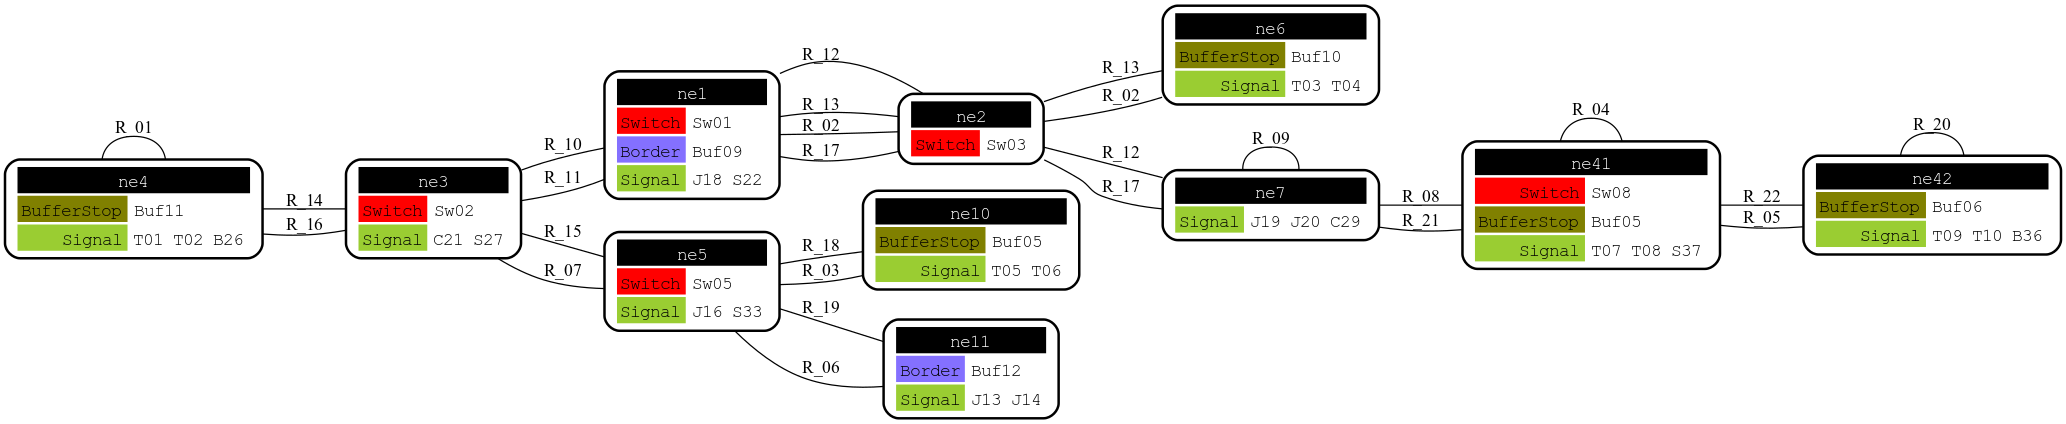
\includegraphics[origin = c, width=\textwidth]{Figuras/Graph_6}
		\centering\caption{Red de grafos generada por el RNA para el ejemplo 6.}
		\label{fig:EJ6_8}
	\end{figure}
	
	Cada nodo del grafo de la Figura \ref{fig:EJ6_8} corresponde a un \textit{netElement}. En cada nodo se listan todos los elementos ferroviarios contenidos por en \textit{netElement}. Las aristas del grafo son las rutas que los conectan. De esta manera, es posible detectar visualmente cualquier nodo aislado de la red o nodos que solo son accedidos en un sentido. Por ejemplo, si entre dos nodos no existe una cantidad par de rutas, entonces solamente se puede circular entre esos nodos en un solo sentido.
    \section{Sistema generado por el ACG}
	
	En base a la red de grafos, ilustrada en la Figura \ref{fig:EJ6_8}, el ACG determinó la siguiente cantidad de elementos, tal puede visualizarse en el Código \ref{lst:EJ6_8}.
	
	\begin{lstlisting}[language = {}, caption = Cantidad de elementos a implementar por el ACG, label = {lst:EJ6_8}]
	n_netElements:11
	n_switch:5
	n_doubleSwitch:0
	n_borders:2
	n_buffers:5
	n_levelCrossings:0
	n_platforms:0
	n_scissorCrossings:0
	n_signals:24
	N : 62
	\end{lstlisting}
	
	Se repetirán los pasos detallados en el ejemplo 1, Sección \ref{sec:EJEMPLO1_ACG}, por lo que solamente se destacarán aspectos particulares de este ejemplo. El ACG genera 80 archivos en formato VHDL. El archivo \textit{Arty\_Z7-10.XDC} es el mismo para todos los ejemplos, al ser invariante respecto a la cantidad de pines a utilizar. Se deberá modificar el script mostrado en el Código \ref{lst:EJ1_script} y cambiar el parámetro \textit{chosen} a 6 para automatizar la importación de los archivos del ejemplo 6 y desvincular cualquier otro conjunto de archivos de ejemplos anteriores.
	
	Una vez ejecutado el script, Vivado ordenará los archivos de forma jerárquica, donde el módulo \textit{global} incluye todos los módulos que fueron detallados en la Sección \ref{sec:interlockingArch}. Cada una de las instancias del módulo \textit{network} contienen sus propias 62 instancias de los mismos módulos de cada elemento ferroviario ya que N, cantidad de elementos ferroviarios, es 62 en el Código \ref{lst:EJ6_8}. El ejemplo 6 utiliza mas de 19870 sub módulos conectados automáticamente mediante mas de 37910 señales, lo cual se aleja bastante de un desarrollo que pueda realizarse manualmente de forma trivial.
	
	Cuando Vivado genera el diagrama de bloques ya tenemos la certeza de que el código VHDL ha pasado la prueba de sintaxis del entorno de desarrollo. A continuación, se deberá sintetizar e implementar el sistema para generar el bitstream que será utilizado para programar la FPGA. Los procesos de síntesis e implementación fueron detallados en el ejemplo 1, Sección \ref{sec:EJEMPLO1_ACG}.
	
	Los resultados de ambos procesos son detallados en la Tabla \ref{Tab:tabla_ACG_6}. Los porcentajes de uso son calculados por Vivado automáticamente, teniendo en cuenta que la plataforma Arty Z7 20 posee 53200 Look-Up-Tables (LUTs), 106400 Flip-Flops (FFs), 125 Pines de entrada y salida (IOs) y 32 Buffers (BUFGs), tal cómo se explicó en la Sección \ref{sec:AGG}. En este ejemplo, la cantidad de recursos utilizados es baja y el tiempo de síntesis e implementación es de 49 y 1 minuto con 10 segundos, respectivamente.
	
	\begin{table}[H]
		{
			\caption{Síntesis e implementación del ejemplo 6 generado por el ACG.}
			\label{Tab:tabla_ACG_6}
			\centering
			%\small
			%\centering
			\begin{center}
				\resizebox{0.7\textwidth}{!}{
					\begin{tabular}{ c c c c }
						\hline	
						Recursos & Síntesis & Implementación & Uso \\	
						\hline
						LUT & 3388 & 3348 & 6.37-6.29\%\\
						FF & 3793 & 3796 & 3.56-3.57\%\\
						IO & 15 & 15 & 12.00\%\\
						BUFG & 3 & 3 & 9.38\%\\
						\hline
					\end{tabular}
				}
			\end{center}
		}    
	\end{table}
    \subsection{Validacion del sistema}

    \lipsum[1]

    \begin{table}[!h]
        {
        \caption{Equivalencias entre las rutas originales y las generadas por el RNA.}
        \label{Tab:tabla_validation_6}
        \centering
        %\small
            %\centering
            \begin{center}
            \resizebox{1\textwidth}{!}{
            \begin{tabular}{ c c c c }
                \hline	
                    Original & Señales & RNA & Señales \\	
                \hline
                    R$_{01}$ & S$_{01}$-S$_{06}$ & R$_{11}$ & S$_{22}$-S$_{27}$ \\
                    R$_{02}$ & S$_{01}$-S$_{13}$ & R$_{13}$ & S$_{22}$-T$_{03}$ \\
                    R$_{03}$ & S$_{01}$-S$_{18}$ & R$_{12}$ & S$_{22}$-J$_{19}$ \\
                    R$_{04}$ & S$_{06}$-S$_{07}$ & R$_{15}$ & S$_{27}$-S$_{33}$ \\
                    R$_{05}$ & S$_{06}$-S$_{12}$ & R$_{16}$ & S$_{27}$-T$_{01}$ \\
                    R$_{06}$ & S$_{21}$-S$_{19}$ & R$_{21}$ & S$_{37}$-J$_{20}$ \\
                    R$_{07}$ & S$_{21}$-S$_{14}$ & R$_{22}$ & S$_{37}$-B$_{36}$ \\
                    R$_{08}$ & S$_{05}$-S$_{02}$ & R$_{10}$ & C$_{21}$-J$_{18}$ \\
                    R$_{09}$ & S$_{09}$-S$_{08}$ & R$_{06}$ & J$_{14}$-J$_{16}$ \\
                    R$_{10}$ & S$_{08}$-S$_{05}$ & R$_{07}$ & J$_{16}$-C$_{21}$ \\
                    R$_{11}$ & S$_{10}$-S$_{08}$ & R$_{03}$ & T$_{06}$-J$_{16}$ \\
                    R$_{12}$ & S$_{15}$-S$_{16}$ & R$_{05}$ & T$_{10}$-T$_{07}$ \\
                    R$_{13}$ & S$_{18}$-S$_{16}$ & R$_{08}$ & J$_{19}$-T$_{07}$ \\
                    R$_{14}$ & S$_{19}$-S$_{20}$ & R$_{08}$ & J$_{20}$-C$_{29}$ \\
                    R$_{15}$ & S$_{20}$-S$_{02}$ & R$_{17}$ & C$_{29}$-J$_{18}$ \\
                    R$_{16}$ & S$_{07}$-S$_{11}$ & R$_{19}$ & S$_{33}$-T$_{05}$ \\
                \hline
            \end{tabular}
            }
            \end{center}
        }    
    \end{table}
	%\section{Ejemplo 7}
      
    \section{Topología ferroviaria original}

	El primer ejemplo, ilustrado en la Figura \ref{fig:EJ7_1}, es una topología diseñada por el autor de esta tesis, en base a múltiples niveles de ramificaciones. La primera ramificación, utilizando los cambios de vías Sw18 y Sw19, es una ramificación doble que lleva a una vía secundaria donde las formaciones pueden maniobrar para volver a la red. La segunda ramificación, utilizando los cambios de vías Sw18 y Sw14, es una ramificación compleja al incluir el cambio de vías Sw14 a continuación del Sw18. Ademas, se incluyeron curvas en los \textit{netElements} ne41 y ne32. El objetivo de este ejemplo fue comprobar el funcionamiento del RNA con una topología de múltiples ramificaciones que llevan a vías sin salida.	Para mas detalles de este ejemplo, incluyendo las figuras, tablas y explicaciones paso a paso, consultar el repositorio de GitHub \cite{GITHUB_PHD}.
	
	\begin{figure}[h]
		\centering
		\includegraphics[width=1\textwidth]{resultados-obtenidos/ejemplo7/images/7_empty.png}
		\centering\caption{Topología ferroviaria del ejemplo 7 sin señalamiento.}
		\label{fig:EJ7_1}
	\end{figure}
	
	Para incrementar la dificultad del análisis y obtener resultados mas completos, todos los finales de vías son absolutos. No se incluyeron plataformas ni cruces de vías. La distribución de los cambios de vías se diseñó para abarcar la mayor cantidad de casos posibles.
    \subsection{Señalamiento original}

    \lipsum[1]
    
    \begin{table}[!h]
        {
        \caption{Tabla de enclavamiento original del ejemplo 7.}
        \label{Tab:tabla_original_7}
        \centering
        \resizebox{1\textwidth}{!}{
            \begin{tabular}{ c c c c c c c }
                \hline	
                    Ruta & Inicio & Final & Cambio & Plataforma & Cruce & netElement \\	
                \hline
                    R$_{01}$  & S$_{01}$ & S$_{02}$ & Sw$_{18}^{N}$ & - & - & ne$_{01}$-ne$_{41}$\\
                    R$_{02}$  & S$_{01}$ & S$_{06}$ & Sw$_{14}^{N}$+Sw$_{18}^{R}$ & - & - & ne$_{01}$-ne$_{32}$\\
                    R$_{03}$  & S$_{01}$ & S$_{07}$ & Sw$_{14}^{R}$+Sw$_{18}^{R}$ & - & - & ne$_{01}$-ne$_{31}$\\
                    R$_{04}$  & S$_{03}$ & S$_{09}$ & Sw$_{19}^{N}$ & - & - & ne$_{42}$-ne$_{43}$\\
                    R$_{05}$  & S$_{03}$ & S$_{10}$ & Sw$_{18}^{N}$+Sw$_{19}^{R}$ & - & - & ne$_{42}$-ne$_{01}$\\
                    R$_{06}$  & S$_{02}$ & S$_{08}$ & Sw$_{19}^{R}$ & - & - & ne$_{41}$-ne$_{42}$\\
                    R$_{07}$  & S$_{04}$ & S$_{10}$ & Sw$_{14}^{R}$+Sw$_{18}^{R}$ & - & - & ne$_{31}$-ne$_{01}$\\
                    R$_{08}$  & S$_{05}$ & S$_{10}$ & Sw$_{14}^{N}$+Sw$_{18}^{R}$ & - & - & ne$_{32}$-ne$_{01}$\\
                \hline
            \end{tabular}
        }
     }
    \end{table}
    \subsection{Generación de señalamiento paso a paso}

	Al ejecutar el RNA, primero detectará todos los \textit{netElements}, sus coordenadas iniciales y finales en la topología, y el sentido en el que fueron definidas. El resultado obtenido se muestra en el Cóodigo \ref{lst:EJ7_1}.
	
	\begin{lstlisting}[language = {}, caption = Detección de \textit{netElements} por parte del RNA , label = {lst:EJ7_1}]
	###### Starting Railway Network Analyzer #####
	Reading .railML file
	Creating railML object
	Analyzing railML object
	Analyzing graph
	ne1 [-770, -30] [260, -30] >>
	ne31 [554, 480] [1190, 480] >>
	ne32 [554, 480] [1460, 957] >>
	ne40 [260, -30] [554, 480] >>
	ne41 [260, -30] [1040, -420] >>
	ne42 [1040, -420] [1730, -420] >>
	ne43 [1040, -420] [440, -420] <<
	The network is connected
	\end{lstlisting}
	
	Por ejemplo, el \textit{netElement} ne42 inicia en la coordenada (1040;-420) y finaliza en la coordenada (1730;-420). El símbolo $>>$ indica que ne1 se encuentra definido de izquierda a derecha, ya que la componente x de la coordenada final es mayor a la de la coordenada inicial, teniendo la misma componente y. Además, se puede comprobar que la lista obtenida en consistente con la Figura \ref{fig:EJ7_2}. Por ejemplo, ne1, ne40 y ne41 comparten la coordenada (260;-30), que coincide con la coordenada del cambio de vías Sw18.
	
	A continuación, el RNA detectará la infraestructura ferroviaria, las curvas peligrosas y los puntos medios de los netElements que el RNA considera demasiado largos. El resultado de este proceso se puede visualizar en el Código \ref{lst:EJ7_2} y puede leerse también en el archivo Infrastructure.RNA.
	
	\begin{lstlisting}[language = {}, caption = Detección de puntos críticos por parte del RNA , label = {lst:EJ7_2}]
	Analyzing infrastructure --> Infrastructure.RNA
	Detecting Danger --> Safe_points.RNA
	ne1 has a Middle point @ [-564.0, -30]
	ne1 has a Middle point @ [-358.0, -30]
	ne1 has a Middle point @ [-152.0, -30]
	ne1 has a Middle point @ [54.0, -30]
	ne31 has a Middle point @ [766.0, 480]
	ne31 has a Middle point @ [978.0, 480]
	ne32 has a Curve(2 lines) @ [[830, 957]]
	ne41 has a Curve(2 lines) @ [[650, -30]]
	ne42 has a Middle point @ [1270.0, -420]
	ne42 has a Middle point @ [1500.0, -420]
	ne43 has a Middle point @ [640.0, -420]
	ne43 has a Middle point @ [840.0, -420]
	\end{lstlisting}
	
	Una vez que el RNA detectó cada punto crítico de la red ferroviaria, procede a generar el señalamiento. El orden de generación no es importante, pero para poder describirlo de forma consistente se iniciará generando el señalamiento para proteger los finales de vías, las junturas entre rieles, las plataformas, los cruces de vía y los cambios de vías. Luego se procederá a mostrar el señalamiento pre y post simplificación. Las señales generadas para proteger los finales de vías relativos y absolutos son ilustradas en la Figura \ref{fig:EJ7_3}.
	
	\begin{figure}[H]
		\centering
		\includegraphics[width=1\textwidth]{resultados-obtenidos/ejemplo7/images/7_step1.png}
		\centering\caption{Señalamiento generado por el RNA para proteger el fin de vía.}
		\label{fig:EJ7_3}
	\end{figure}
	
	Los finales de vías absolutos son protegidos por las señales de parada T01, T03, T05, T07 y T09; y las señales de partida son T02, T04, T06, T08 y T10. No existen finales de vías relativos que proteger, por lo que el RNA asigno señalamiento para ese fin. Al tampoco existir junturas que proteger, la Figura \ref{fig:EJ7_4} no presenta cambios.
	
	\begin{figure}[H]
		\centering
		\includegraphics[width=1\textwidth]{resultados-obtenidos/ejemplo7/images/7_step2.png}
		\centering\caption{Señalamiento generado por el RNA para proteger las junturas.}
		\label{fig:EJ7_4}
	\end{figure}
	
	Al generar el señalamiento para proteger la infraestructura, tal como se explicó en la Sección \ref{sec:horizontal}, el Algoritmo \ref{alg:horizontal} simplificará las señales entre dos elementos ferroviarios si no existe espacio suficiente entre ellos. Al no existir plataformas o cruces de vías el señalamiento que se ilustra en la Figura \ref{fig:EJ7_5} no presenta cambios.
	
	\begin{figure}[H]
		\centering
		\includegraphics[width=1\textwidth]{resultados-obtenidos/ejemplo7/images/7_step3.png}
		\centering\caption{Señalamiento generado por el RNA para proteger plataformas y cruces de vía.}
		\label{fig:EJ7_5}
	\end{figure}
	
	El RNA generó las señales S14, C13 y H15 para proteger el cambio de vías Sw18; las señales C11, B12 y H16 para proteger el cambio de vías Sw14 y las señales S19, C17, B18 y H20 para proteger el cambio de vías Sw19. Las señales mencionadas se encuentran resaltadas en rojo en la Figura \ref{fig:EJ7_6}.
	
	\begin{figure}[H]
		\centering
		\includegraphics[width=1\textwidth]{resultados-obtenidos/ejemplo7/images/7_step4.png}
		\centering\caption{Señalamiento generado por el RNA para proteger los cambios de vías.}
		\label{fig:EJ7_6}
	\end{figure}
	
	Una vez obtenido todo el señalamiento, el RNA procede a simplificar las señales redundantes, repetidas o cuyas funciones o ubicaciones se superponen entre sí. El proceso de simplificación de señales fue explicado en la Sección \label{sec:simplificacion}. El Algoritmo \ref{alg:vertical} de herencia vertical fue aplicado en las señales B entre los cambios de vías Sw18 y Sw19, desplazando las señales hasta convertirlas en las señales B12 y B18 respectivamente. Análogamente, las señales C y S del \textit{netElement} se convirtieron en las señales H15 y C17 respectivamente.
	
	Las señales simplificadas al aplicar el Algoritmo \ref{alg:horizontal} de herencia horizontal son: C11, B12, H15, H16, C17, C13, S19 y H20. Las señales H15 y H16 fueron eliminadas por su cercanía con la señal S14, con la cual comparten dirección y sentido. Lo mismo ocurre entre las señales H20 y C13. En todos los casos, se aplicó el Algoritmo \ref{alg:horizontal}, diseñado para agrupar objetos cercanos como un único objeto, generando el señalamiento acorde a los elementos contenidos en cada extremo del nuevo elemento contenedor.
	
	Finalmente, las señales son simplificadas aplicando el Algoritmo \ref{alg:reduction} de eliminación por prioridad de señales. El resultado de este proceso es detallado en el Código \ref{lst:EJ7_3}.
	
	\begin{lstlisting}[language = {}, caption = Reducción de señalamiento por prioridad de señales, label = {lst:EJ7_3}]
	Reducing redundant signals
	T priority removing sig12 for sig04
	T priority removing sig11 for sig06
	T priority removing sig13 for sig08
	T priority removing sig19 for sig08
	T priority removing sig17 for sig10
	Same position removing sig15 for sig14
	Same position removing sig16 for sig14
	Same position removing sig20 for sig13
	\end{lstlisting}
	
	El resultado de la simplificación del señalamiento se ilustra en la Figura \ref{fig:EJ7_7}.
	
	\begin{figure}[H]
		\centering
		\includegraphics[width=1\textwidth]{resultados-obtenidos/ejemplo7/images/7_RNA.png}
		\centering\caption{Señalamiento generado y simplificado por el RNA.}
		\label{fig:EJ7_7}
	\end{figure}
	
	Al finalizar la generación del señalamiento, el RNA debe detectar todas las posibles rutas admitidas por la red para crear la tabla de enclavamientos. El RNA exporta los resultados del análisis en los siguientes cuatro documentos: Infrastructure.RNA (Apéndice \ref{sec:infrastructureRNA}), SafePoint.RNA (Apéndice \ref{sec:safePointsRNA}), Signalling.RNA (Apéndice \ref{sec:signallingRNA}) y Routes.RNA (Apéndice \ref{sec:routesRNA}).
    \subsection{Red de grafos generada por el RNA}

	La información exportada en el Código \ref{lst:EJ7_5}, Código \ref{lst:EJ7_6} y Código \ref{lst:EJ7_7} es utilizada resumida por el RNA para una mejor interpretación. El resultado de este resumen se ilustra en el diagrama de la Figura \ref{fig:EJ7_8}.

	\begin{figure}[H]
		\centering
		\includegraphics[width=1\textwidth]{Figuras/Graph_7}
		\centering\caption{Red de grafos generada por el RNA para el ejemplo 7.}
		\label{fig:EJ7_8}
	\end{figure}
	
	Cada nodo del grafo de la Figura \ref{fig:EJ1_8} corresponde a un \textit{netElement}. En cada nodo se listan todos los elementos ferroviarios contenidos por en \textit{netElement}. Las aristas del grafo son las rutas que los conectan. De esta manera, es posible detectar visualmente cualquier nodo aislado de la red o nodos que solo son accedidos en un sentido. Por ejemplo, si algún entre dos nodos no existe una cantidad par de rutas, entonces solamente se puede circular entre esos nodos en un solo sentido.
    \section{Señalamiento generado por el RNA}

    El RNA también exporta la misma información mostrada en el Código \ref{lst:EJ7_8} en una hoja de cálculo, similar a la que se visualiza en la Tabla \ref{Tab:tabla_generated_7}.
    
    \begin{table}[H]
        {
        \caption{Tabla de enclavamiento del ejemplo 7 generada por el RNA.}
        \label{Tab:tabla_generated_7}
        \centering
        \resizebox{1\textwidth}{!}{
            \begin{tabular}{ c c c c c c c }
                \hline	
                    Ruta & Inicio & Final & Cambio & Plataforma & Cruce & netElement \\	
                \hline
                    R$_{01}$  & T$_{02}$ & S$_{14}$ & - & - & - & ne$_{01}$\\
                    R$_{02}$  & T$_{04}$ & T$_{01}$ & Sw$_{14}^{R}$+Sw$_{18}^{R}$ & - & - & ne$_{31}$-ne$_{01}$\\
                    R$_{03}$  & T$_{06}$ & T$_{01}$ & Sw$_{14}^{N}$+Sw$_{18}^{R}$ & - & - & ne$_{32}$-ne$_{01}$\\
                    R$_{04}$  & T$_{08}$ & H$_{20}$ & - & - & - & ne$_{42}$\\
                    R$_{05}$  & T$_{10}$ & T$_{07}$ & Sw$_{19}^{N}$ & - & - & ne$_{43}$-ne$_{42}$\\
                    R$_{06}$  & S$_{14}$ & B$_{18}$ & Sw$_{18}^{N}$ & - & - & ne$_{01}$-ne$_{41}$\\
                    R$_{07}$  & S$_{14}$ & T$_{05}$ & Sw$_{18}^{R}$+Sw$_{14}^{N}$ & - & - & ne$_{01}$-ne$_{32}$\\
                    R$_{08}$  & S$_{14}$ & T$_{03}$ & Sw$_{18}^{R}$+Sw$_{14}^{R}$ & - & - & ne$_{01}$-ne$_{31}$\\
                    R$_{09}$  & B$_{18}$ & T$_{07}$ & Sw$_{19}^{R}$ & - & - & ne$_{41}$-ne$_{42}$\\
                    R$_{10}$  & H$_{20}$ & T$_{09}$ & Sw$_{19}^{N}$ & - & - & ne$_{42}$-ne$_{43}$\\
                    R$_{11}$  & H$_{20}$ & T$_{01}$ & Sw$_{19}^{R}$+Sw$_{18}^{N}$ & - & - & ne$_{42}$-ne$_{01}$\\
                \hline
            \end{tabular}
        }
     }
    \end{table}
    
    En una primera inspección podemos ver que el nuevo señalamiento tiene 11 rutas, versus las 8 rutas del señalamiento original (ver Tabla \ref{Tab:tabla_original_7}). Esto se debe a que el RNA añade protecciones extras para los finales de vía absolutos, ausentes en el señalamiento original.
    \section{Sistema generado por el ACG}

	En base a la red de grafos, ilustrada en la Figura \ref{fig:EJ7_8}, el ACG determinó la siguiente cantidad de elementos, tal puede visualizarse en el Código \ref{lst:EJ7_8}.
	
	\begin{lstlisting}[language = {}, caption = Cantidad de elementos a implementar por el ACG, label = {lst:EJ7_8}]
	n_netElements:7
	n_switch:3
	n_doubleSwitch:0
	n_borders:0
	n_buffers:5
	n_levelCrossings:0
	n_platforms:0
	n_scissorCrossings:0
	n_signals:13
	N : 34
	\end{lstlisting}
	
	Se repetirán los pasos detallados en el ejemplo 1, Sección \ref{sec:EJEMPLO1_ACG}, por lo que solamente se destacarán aspectos particulares de este ejemplo. El ACG genera 52 archivos en formato VHDL. El archivo \textit{Arty\_Z7-10.XDC} es el mismo para todos los ejemplos, al ser invariante respecto a la cantidad de pines a utilizar. Se deberá modificar el script mostrado en el Código \ref{lst:EJ1_script} y cambiar el parámetro \textit{chosen} a 7 para automatizar la importación de los archivos del ejemplo 7 y desvincular cualquier otro conjunto de archivos de ejemplos anteriores.

	Una vez ejecutado el script, Vivado ordenará los archivos de forma jerárquica, donde el módulo \textit{global} incluye todos los módulos que fueron detallados en la Sección \ref{sec:interlockingArch}. Cada una de las instancias del módulo \textit{network} contienen sus propias 34 instancias de los mismos módulos de cada elemento ferroviario ya que N, cantidad de elementos ferroviarios, es 34 en el Código \ref{lst:EJ7_8}. El ejemplo 7 utiliza mas de 10800 sub módulos conectados automáticamente mediante mas de 21150 señales, lo cual se aleja bastante de un desarrollo que pueda realizarse manualmente de forma trivial.
	
	Cuando Vivado genera el diagrama de bloques ya tenemos la certeza de que el código VHDL ha pasado la prueba de sintaxis del entorno de desarrollo. A continuación, se deberá sintetizar e implementar el sistema para generar el bitstream que será utilizado para programar la FPGA. Los procesos de síntesis e implementación fueron detallados en el ejemplo 1, Sección \ref{sec:EJEMPLO1_ACG}.
	
	Los resultados de ambos procesos son detallados en la Tabla \ref{Tab:tabla_ACG_7}. Los porcentajes de uso son calculados por Vivado automáticamente, teniendo en cuenta que la plataforma Arty Z7 20 posee 53200 Look-Up-Tables (LUTs), 106400 Flip-Flops (FFs), 125 Pines de entrada y salida (IOs) y 32 Buffers (BUFGs), tal cómo se explicó en la Sección \ref{sec:AGG}. En este ejemplo, la cantidad de recursos utilizados es baja y el tiempo de síntesis e implementación es de 35 y 54 segundos, respectivamente.
	
	\begin{table}[H]
		{
			\caption{Síntesis e implementación del ejemplo 7 generado por el ACG.}
			\label{Tab:tabla_ACG_7}
			\centering
			%\small
			%\centering
			\begin{center}
				\resizebox{0.65\textwidth}{!}{
					\begin{tabular}{ c c c c }
						\hline	
						Recursos & Síntesis & Implementación & Uso \\	
						\hline
						LUT & 1824 & 1798 & 3.43-3.38\%\\
						FF & 2008 & 2011 & 1.89\%\\
						IO & 15 & 15 & 12.00\%\\
						BUFG & 3 & 3 & 9.38\%\\
						\hline
					\end{tabular}
				}
			\end{center}
		}    
	\end{table}
    \subsection{Validacion del sistema}

    \lipsum[1]

    \begin{table}[H]
        {
        \caption{Equivalencias entre las rutas originales y las generadas por el RNA.}
        \label{Tab:tabla_validation_7}
        \centering
        %\small
            %\centering
            \begin{center}
            \resizebox{1\textwidth}{!}{
            \begin{tabular}{ c c c c }
                \hline	
                    Original & Señales & RNA & Señales \\	
                \hline
                    R$_{01}$ & S$_{01}$-S$_{02}$ & R$_{06}$ & S$_{14}$-B$_{18}$ \\
                    R$_{02}$ & S$_{01}$-S$_{06}$ & R$_{07}$ & S$_{14}$-T$_{05}$ \\
                    R$_{03}$ & S$_{01}$-S$_{07}$ & R$_{08}$ & S$_{14}$-T$_{03}$ \\
                    R$_{04}$ & S$_{03}$-S$_{09}$ & R$_{09}$ & B$_{18}$-T$_{07}$ \\
                    R$_{05}$ & S$_{03}$-S$_{10}$ & R$_{11}$ & H$_{20}$-T$_{09}$ \\
                    R$_{06}$ & S$_{02}$-S$_{08}$ & R$_{10}$ & H$_{20}$-T$_{01}$ \\
                    R$_{07}$ & S$_{04}$-S$_{10}$ & R$_{02}$ & T$_{04}$-T$_{01}$ \\
                    R$_{08}$ & S$_{05}$-S$_{10}$ & R$_{03}$ & T$_{06}$-T$_{01}$ \\
                \hline
            \end{tabular}
            }
            \end{center}
        }    
    \end{table}
    
    \lipsum[1]
	%\chapter{Ejemplo 8}
	\label{sec:ejemplo_8}
	
    \subsection{Topología ferroviaria original}

	El primer ejemplo, ilustrado en la Figura \ref{fig:EJ8_1}, es una topología diseñada en base a dos líneas principales conectadas por un cambio de vías y seis cruces de vías. Los cambios de vías Sw11 y Sw12 permiten el intercambio de formaciones entre ambas vías principales. El objetivo de este ejemplo fue comprobar el funcionamiento del RNA con una topología de doble vía conectadas por dos cambios de vías, similares a las que se pueden encontrar en estaciones reales.
	
	\begin{figure}[h]
		\centering
		\includegraphics[width=1\textwidth]{resultados-obtenidos/ejemplo8/images/8_empty.png}
		\centering\caption{Topología ferroviaria del ejemplo 8 sin señalamiento.}
		\label{fig:EJ8_1}
	\end{figure}
	
	Para incrementar la dificultad del análisis y obtener resultados mas completos, todos los finales de vías son relativos y se añadieron las plataformas (Plat01, Plat02) y cruces de vías (Lc03, Lc04, Lc05, Lc06, Lc07, LC09). La infraestructura se distribuyó de forma tal de tener que en algunos casos el espacio entre ambos fuese suficiente (Lc04 y Plat01) y en otros no (Lc07 y Plat02).

    \subsection{Señalamiento original}

    \lipsum[1]
    
    \begin{table}[H]
        {
        \caption{Tabla de enclavamiento original del ejemplo 8.}
        \label{Tab:tabla_original_8}
        \centering
        \resizebox{1\textwidth}{!}{
            \begin{tabular}{ c c c c c c c }
                \hline	
                    Ruta & Inicio & Final & Cambio & Plataforma & Cruce & netElement \\	
                \hline
                    R$_{01}$  & S$_{06}$ & S$_{16}$ & - & Plat$_{01}$ & Lc$_{03}$ & ne$_{26}$\\
                    R$_{02}$  & S$_{07}$ & S$_{05}$ & - & Plat$_{01}$ & Lc$_{04}$ & ne$_{26}$\\
                    R$_{03}$  & S$_{08}$ & S$_{10}$ & - & Plat$_{02}$ & Lc$_{07}$ & ne$_{23}$\\
                    R$_{04}$  & S$_{10}$ & S$_{12}$ & Sw$_{11}^{N}$ & - & Lc$_{09}$ & ne$_{23}$-ne$_{25}$\\
                    R$_{05}$  & S$_{10}$ & S$_{14}$ & Sw$_{11}^{R}$+Sw$_{12}^{R}$ & - & Lc$_{09}$ & ne$_{23}$-ne$_{03}$\\
                    R$_{06}$  & S$_{11}$ & S$_{09}$ & - & Plat$_{02}$ & Lc$_{09}$ & ne$_{23}$\\
                    R$_{07}$  & S$_{12}$ & S$_{03}$ & - & - & Lc$_{05}$ & ne$_{25}$\\
                    R$_{08}$  & S$_{13}$ & S$_{11}$ & - & - & Lc$_{05}$ & ne$_{25}$-ne$_{23}$\\
                    R$_{09}$  & S$_{14}$ & S$_{01}$ & - & - & Lc$_{06}$ & ne$_{03}$\\
                    R$_{10}$  & S$_{15}$ & S$_{07}$ & Sw$_{12}^{N}$ & - & Lc$_{06}$ & ne$_{03}$-ne$_{26}$\\
                    R$_{11}$  & S$_{15}$ & S$_{11}$ & Sw$_{11}^{R}$+Sw$_{12}^{N}$ & - & Lc$_{06}$ & ne$_{03}$-ne$_{23}$\\
                    R$_{12}$  & S$_{16}$ & S$_{14}$ & - & - & Lc$_{04}$ & ne$_{26}$-ne$_{03}$\\
                \hline
            \end{tabular}
        }
     }
    \end{table}
    
    \lipsum[1]
    \subsection{Generación de señalamiento paso a paso}

	Al ejecutar el RNA, primero detectará todos los \textit{netElements}, sus coordenadas iniciales y finales en la topología, y el sentido en el que fueron definidas. El resultado obtenido se muestra en el Cóodigo \ref{lst:EJ8_1}.
	
	\begin{lstlisting}[language = {}, caption = Detección de \textit{netElements} por parte del RNA , label = {lst:EJ8_1}]
	###### Starting Railway Network Analyzer #####
	Reading .railML file
	Creating railML object
	Analyzing railML object
	Analyzing graph
	ne3 [2040, 120] [1020, 120] <<
	ne23 [-960, -300] [600, -300] >>
	ne25 [600, -300] [2040, -300] >>
	ne26 [1020, 120] [-960, 120] <<
	ne27 [600, -300] [1020, 120] >>
	The network is connected
	\end{lstlisting}
	
	Por ejemplo, el \textit{netElement} ne26 inicia en la coordenada (1020;120) y finaliza en la coordenada (-960;120). El símbolo $<<$ indica que ne1 se encuentra definido de derecha a izquierda, ya que la componente x de la coordenada final es menor a la de la coordenada inicial, teniendo la misma componente y. Además, se puede comprobar que la lista obtenida en consistente con la Figura \ref{fig:EJ8_2}. Por ejemplo, ne03, ne26 y ne27 comparten la coordenada (1020;120), que coincide con la coordenada del cambio de vías Sw12.
	
	A continuación, el RNA detectará la infraestructura ferroviaria, las curvas peligrosas y los puntos medios de los netElements que el RNA considera demasiado largos. El resultado de este proceso se puede visualizar en el Código \ref{lst:EJ8_2} y puede leerse también en el archivo Infrastructure.RNA.
	
	\begin{lstlisting}[language = {}, caption = Detección de puntos críticos por parte del RNA , label = {lst:EJ8_2}]
	Analyzing infrastructure --> Infrastructure.RNA
	Detecting Danger --> Safe_points.RNA
	ne3 has a LevelCrossing[Lc06] @ [1536, -120]
	ne23 has a Platform[Plat02] @ [-160, 300]
	ne23 has a LevelCrossing[Lc07] @ [-494, 300]
	ne23 has a LevelCrossing[Lc09] @ [266, 300]
	ne25 has a LevelCrossing[Lc05] @ [1166, 300]
	ne26 has a Platform[Plat01] @ [-41, -120]
	ne26 has a LevelCrossing[Lc03] @ [-404, -120]
	ne26 has a LevelCrossing[Lc04] @ [572, -120]
	\end{lstlisting}
	
	Una vez que el RNA detectó cada punto crítico de la red ferroviaria, procede a generar el señalamiento. El orden de generación no es importante, pero para poder describirlo de forma consistente se iniciará generando el señalamiento para proteger los finales de vías, las junturas entre rieles, las plataformas, los cruces de vía y los cambios de vías. Luego se procederá a mostrar el señalamiento pre y post simplificación. Las señales generadas para proteger los finales de vías relativos y absolutos son ilustradas en la Figura \ref{fig:EJ8_3}.
	
	\begin{figure}[H]
		\centering
		\includegraphics[width=1\textwidth]{resultados-obtenidos/ejemplo8/images/8_step1.png}
		\centering\caption{Señalamiento generado por el RNA para proteger el fin de vía.}
		\label{fig:EJ8_3}
	\end{figure}
	
	Al no existir finales de vías absolutos, el RNA no les asignó señalamiento. En cambio, los finales de vías relativos poseen las señales de parada L01, L02, L03 y L04, cercanos al límite del externo del \textit{netElement} al que pertenecen.
	
	La Figura \ref{fig:EJ8_4} no presenta cambios en el señalamiento, al no existir junturas entre los rieles que proteger.
	
	\begin{figure}[H]
		\centering
		\includegraphics[width=1\textwidth]{resultados-obtenidos/ejemplo8/images/8_step2.png}
		\centering\caption{Señalamiento generado por el RNA para proteger las junturas.}
		\label{fig:EJ8_4}
	\end{figure}
	
	Al generar el señalamiento para proteger la infraestructura, tal como se explicó en la Sección \ref{sec:horizontal}, el Algoritmo \ref{alg:horizontal} simplificará las señales entre dos elementos ferroviarios si no existe espacio suficiente entre ellos, tal como sucede con los elementos Lc03 y Plat01. El señalamiento generado para proteger las plataformas y los cruces de vía se ilustra en rojo en la Figura \ref{fig:EJ8_5}. Las señales generadas para proteger las plataformas son las señales de partida P17, P18, P19 y P20, mientras que las señales que protegen los cruces de vía son todas las señales entre X05 y X16.
	
	\begin{figure}[H]
		\centering
		\includegraphics[width=1\textwidth]{resultados-obtenidos/ejemplo8/images/8_step3.png}
		\centering\caption{Señalamiento generado por el RNA para proteger plataformas y cruces de vía.}
		\label{fig:EJ8_5}
	\end{figure}
	
	El RNA generó las señales S22, C21 y H23 para proteger el cambio de vías Sw11 y las señales S25, C24 y H26 para proteger el cambio de vías Sw12. Las señales mencionadas se encuentran resaltadas en rojo en la Figura \ref{fig:EJ8_6}.
	
	\begin{figure}[H]
		\centering
		\includegraphics[width=1\textwidth]{resultados-obtenidos/ejemplo8/images/8_step4.png}
		\centering\caption{Señalamiento generado por el RNA para proteger los cambios de vías.}
		\label{fig:EJ8_6}
	\end{figure}
	
	Una vez obtenido todo el señalamiento, el RNA procede a simplificar las señales redundantes, repetidas o cuyas funciones o ubicaciones se superponen entre sí. El proceso de simplificación de señales fue explicado en la Sección \label{sec:simplificacion}. El Algoritmo \ref{alg:vertical} de herencia vertical fue aplicado en las señales B entre los cambios de vías Sw11 y Sw12, desplazando las señales hasta convertirlas en las señales H33 y H36 respectivamente.
	
	Las señales simplificadas al aplicar el Algoritmo \ref{alg:horizontal} de herencia horizontal son: X11, H23, P18, X08, H26, X15, S19, P17 y X10. Las señales P20, X11 y H23 fueron eliminadas por su cercanía con la señal S22, con la cual comparten dirección y sentido. Lo mismo ocurre entre las señales H26 y X15. En todos los casos, se aplicó el Algoritmo \ref{alg:horizontal}, diseñado para agrupar objetos cercanos como un único objeto, generando el señalamiento acorde a los elementos contenidos en cada extremo del nuevo elemento contenedor.
	
	Finalmente, las señales son simplificadas aplicando el Algoritmo \ref{alg:reduction} de eliminación por prioridad de señales. El resultado de este proceso es detallado en el Código \ref{lst:EJ8_3}.
	
	\begin{lstlisting}[language = {}, caption = Reducción de señalamiento por prioridad de señales, label = {lst:EJ8_3}]
	Reducing redundant signals
	removing sig17 for sig05
	removing sig18 for sig08
	removing sig08 for sig24
	removing sig10 for sig19
	removing sig11 for sig22
	removing sig21 for sig14
	removing sig15 for sig25
	removing sig20 for sig22
	removing sig23 for sig22
	removing sig26 for sig25
	\end{lstlisting}
	
	El resultado de la simplificación del señalamiento se ilustra en la Figura \ref{fig:EJ8_7}.
	
	\begin{figure}[H]
		\centering
		\includegraphics[width=1\textwidth]{resultados-obtenidos/ejemplo8/images/8_RNA.png}
		\centering\caption{Señalamiento generado y simplificado por el RNA.}
		\label{fig:EJ8_7}
	\end{figure}
	
	Al finalizar la generación del señalamiento, el RNA debe detectar todas las posibles rutas admitidas por la red para crear la tabla de enclavamientos. El RNA exporta los resultados del análisis en los siguientes cuatro documentos:
	
	Infrastructure.RNA (Código \ref{lst:EJ8_4}): resumen de cada elemento ferroviario en cada \textit{netElement}.
	
	\begin{lstlisting}[language = {}, caption = Infrastructure.RNA, label = {lst:EJ8_4}]
	Nodes: 5|Switches: 2|Signals: 0|Detectors: 0|Ends: 4|Barriers: 6
	Node ne3:
		Track = track2
		Neighbours = 2 -> ['ne26', 'ne27']
		Level crossing -> Lc06
		Protection -> true | Barriers -> none | Lights -> none Acoustic -> none
		Position -> [1491, -120] | Coordinate: 0.5373
		Switches -> Sw12
			ContinueCourse -> right -> ne26
			BranchCourse -> left -> ne27
	Node ne23:
		Track = track3
		Neighbours = 2 -> ['ne25', 'ne27']
		Level crossing -> Lc07
		Protection -> true | Barriers -> none | Lights -> none Acoustic -> none
		Position -> [-449, 300] | Coordinate: 0.3273
		Level crossing -> Lc09
		Protection -> true | Barriers -> none | Lights -> none Acoustic -> none
		Position -> [311, 300] | Coordinate: 0.8148
		Switches -> Sw11
			ContinueCourse -> right -> ne25
			BranchCourse -> left -> ne27
	Node ne25:
		Track = track4
		Neighbours = 2 -> ['ne23', 'ne27']
		Level crossing -> Lc05
		Protection -> true | Barriers -> none | Lights -> none Acoustic -> none
		Position -> [1211, 300] | Coordinate: 0.4248
	Node ne26:
		Track = track1
		Neighbours = 2 -> ['ne3', 'ne27']
		Level crossing -> Lc03
		Protection -> true | Barriers -> none | Lights -> none Acoustic -> none
		Position -> [-449, -120] | Coordinate: 0.7421
		Level crossing -> Lc04
		Protection -> true | Barriers -> none | Lights -> none Acoustic -> none
		Position -> [527, -120] | Coordinate: 0.2487
	Node ne27:
		Track = track5
		Neighbours = 4 -> ['ne3', 'ne23', 'ne25', 'ne26']
	\end{lstlisting}
	
	SafePoints.RNA (Código \ref{lst:EJ8_5}): coordenadas absolutas de cada punto donde puede colocarse una señal, en cada \textit{netElement}.
	
	\begin{lstlisting}[language = {}, caption = SafePoints.RNA, label = {lst:EJ8_5}]
	ne3:
		Next: [[1336, -120]]
		Prev: [[1736, -120]]
	ne23:
		Next: [[-360, 300], [-694, 300], [66, 300]]
		Prev: [[40, 300], [-294, 300], [466, 300]]
	ne25:
		Next: [[966, 300]]
		Prev: [[1366, 300]]
	ne26:
		Next: [[-241, -120], [-604, -120], [372, -120]]
		Prev: [[159, -120], [-204, -120], [772, -120]]
	\end{lstlisting}
	
	Signalling.RNA (Código \ref{lst:EJ8_6}): información detallada de todas las señales generadas.
	
	\begin{lstlisting}[language = {}, caption = Signalling.RNA, label = {lst:EJ8_6}]
	sig01 [L01] >>:
		From: ne3 | To: lb70_right
		Type: Circulation | Direction: reverse | AtTrack: right 
		Position: [1940, -120] | Coordinate: 0.9019
	sig02 [L02] <<:
		From: ne23 | To: oe178_left
		Type: Circulation | Direction: reverse | AtTrack: right 
		Position: [-860, 300] | Coordinate: 0.0641
	sig03 [L03] >>:
		From: ne25 | To: oe179_right
		Type: Circulation | Direction: normal | AtTrack: left 
		Position: [1940, 300] | Coordinate: 0.9305
	sig04 [L04] <<:
		From: ne26 | To: lb69_left
		Type: Circulation | Direction: normal | AtTrack: left 
		Position: [-860, -120] | Coordinate: 0.0505
	sig05 [X05] <<:
		From: ne26 | To: ne26_right
		Type: Circulation | Direction: normal | AtTrack: left 
		Position: [-204, 120] | Coordinate: 0.4005
	sig06 [X06] >>:
		From: ne26 | To: ne26_left
		Type: Circulation | Direction: reverse | AtTrack: right 
		Position: [-604, 120] | Coordinate: 0.2168
	sig07 [X07] <<:
		From: ne26 | To: ne26_right
		Type: Circulation | Direction: normal | AtTrack: left 
		Position: [772, 120] | Coordinate: 0.8831
	sig09 [X09] >>:
		From: ne23 | To: ne23_right
		Type: Circulation | Direction: normal | AtTrack: left 
		Position: [-694, -300] | Coordinate: 0.4207
	sig12 [X12] <<:
		From: ne23 | To: ne23_left
		Type: Circulation | Direction: reverse | AtTrack: right 
		Position: [466, -300] | Coordinate: 0.9917
	sig13 [X13] >>:
		From: ne25 | To: ne25_right
		Type: Circulation | Direction: normal | AtTrack: left 
		Position: [966, -300] | Coordinate: 0.4880
	sig14 [X14] <<:
		From: ne25 | To: ne25_left
		Type: Circulation | Direction: reverse | AtTrack: right 
		Position: [1366, -300] | Coordinate: 0.6757
	sig16 [X16] >>:
		From: ne3 | To: ne3_left
		Type: Circulation | Direction: reverse | AtTrack: right 
		Position: [1336, 120] | Coordinate: 0.3890
	sig19 [P19] <<:
		From: ne23 | To: ne23_left
		Type: Circulation | Direction: reverse | AtTrack: right 
		Position: [-280, -300] | Coordinate: 0.5813
	sig22 [S22] >>:
		From: ne23 | To: ne23_right
		Type: Circulation | Direction: normal | AtTrack: left 
		Position: [40, -300] | Coordinate: 0.7475
	sig24 [C24] >>:
		From: ne26 | To: ne26_right
		Type: Circulation | Direction: reverse | AtTrack: right 
		Position: [372, 120] | Coordinate: 0.6835
	sig25 [S25] <<:
		From: ne3 | To: ne3_left
		Type: Circulation | Direction: normal | AtTrack: left 
		Position: [1736, 120] | Coordinate: 0.7403
	\end{lstlisting}
	
	Routes.RNA (Código \ref{lst:EJ8_7}): tabla de enclavamientos.
	
	\begin{lstlisting}[language = {}, caption = Routes.RNA, label = {lst:EJ8_7}]
	route_1 [X05 << L04]:
		Path: ['ne26']
		LevelCrossings: ['Lc03']
	route_2 [X06 >> C24]:
		Path: ['ne26']
		Platforms: ['Plat01']
		LevelCrossings: ['Lc03']
	route_3 [X07 << X05]:
		Path: ['ne26']
		Platforms: ['Plat01']
		LevelCrossings: ['Lc04']
	route_4 [X09 >> S22]:
		Path: ['ne23']
		Platforms: ['Plat02']
		LevelCrossings: ['Lc07']
	route_5 [X12 << P19]:
		Path: ['ne23']
		Platforms: ['Plat02']
		LevelCrossings: ['Lc09']
	route_6 [X13 >> L03]:
		Path: ['ne25']
		LevelCrossings: ['Lc05']
		route_7 [X14 << X12]:
	Path: ['ne25', 'ne23']
		Switches: ['Sw11_N']
		LevelCrossings: ['Lc05']
	route_8 [X16 >> L01]:
		Path: ['ne3']
		LevelCrossings: ['Lc06']
	route_9 [P19 << L02]:
		Path: ['ne23']
		LevelCrossings: ['Lc07']
	route_10 [S22 >> X13]:
		Path: ['ne23', 'ne25']
		Switches: ['Sw11_N']
		LevelCrossings: ['Lc09']
	route_11 [S22 >> X16]:
		Path: ['ne23', 'ne27', 'ne3']
		Switches: ['Sw11_R', 'Sw12_R']
		LevelCrossings: ['Lc09']
	route_12 [C24 >> X16]:
		Path: ['ne26', 'ne3']
		Switches: ['Sw12_N']
		LevelCrossings: ['Lc04']
	route_13 [S25 << X07]:
		Path: ['ne3', 'ne26']
		Switches: ['Sw12_N']
		LevelCrossings: ['Lc06']
	route_14 [S25 << X12]:
		Path: ['ne3', 'ne27', 'ne23']
		Switches: ['Sw11_R', 'Sw12_R']
		LevelCrossings: ['Lc06']
	\end{lstlisting}
    \subsection{Red de grafos generada por el RNA}

 La información exportada en el Código \ref{lst:EJ8_5}, Código \ref{lst:EJ8_6} y Código \ref{lst:EJ8_7} es utilizada resumida por el RNA para una mejor interpretación. El resultado de este resumen se ilustra en el diagrama de la Figura \ref{fig:EJ8_8}.

	\begin{figure}[H]
		\centering
		\includegraphics[width=1\textwidth]{Figuras/Graph_8}
		\centering\caption{Red de grafos generada por el RNA para el ejemplo 8.}
		\label{fig:EJ8_8}
	\end{figure}
	
	Cada nodo del grafo de la Figura \ref{fig:EJ8_8} corresponde a un \textit{netElement}. En cada nodo se listan todos los elementos ferroviarios contenidos por en \textit{netElement}. Las aristas del grafo son las rutas que los conectan. De esta manera, es posible detectar visualmente cualquier nodo aislado de la red o nodos que solo son accedidos en un sentido. Por ejemplo, si algún entre dos nodos no existe una cantidad par de rutas, entonces solamente se puede circular entre esos nodos en un solo sentido.
    \section{Señalamiento generado por el RNA}

    El RNA también exporta la misma información mostrada en el Código \ref{lst:EJ8_8} en una hoja de cálculo, similar a la que se visualiza en la Tabla \ref{Tab:tabla_generated_8}.
    
    \begin{table}[H]
        {
        \caption{Tabla de enclavamiento del ejemplo 8 generada por el RNA.}
        \label{Tab:tabla_generated_8}
        %\centering
        \begin{center}      
        	\resizebox{0.8\textwidth}{!}{
            \begin{tabular}{ c c c c c c c }
                \hline	
                    Ruta & Inicio & Final & Cambio & Plataforma & Cruce & netElement \\	
                \hline
                    R$_{01}$  & X$_{05}$ & L$_{04}$ & - & - & Lc$_{03}$ & ne$_{26}$\\
                    R$_{02}$  & X$_{06}$ & C$_{24}$ & - & Plat$_{01}$ & Lc$_{03}$ & ne$_{26}$\\
                    R$_{03}$  & X$_{07}$ & X$_{05}$ & - & Plat$_{01}$ & Lc$_{04}$ & ne$_{26}$\\
                    R$_{04}$  & X$_{09}$ & S$_{22}$ & - & Plat$_{02}$ & Lc$_{07}$ & ne$_{23}$\\
                    R$_{05}$  & X$_{12}$ & P$_{19}$ & - & Plat$_{02}$ & Lc$_{09}$ & ne$_{23}$\\
                    R$_{06}$  & X$_{13}$ & L$_{03}$ & - & - & Lc$_{05}$ & ne$_{25}$\\
                    R$_{07}$  & X$_{14}$ & X$_{12}$ & Sw$_{11}^{N}$ & - & Lc$_{05}$ & ne$_{25}$-ne$_{23}$\\
                    R$_{08}$  & X$_{16}$ & L$_{01}$ & - & - & Lc$_{06}$ & ne$_{03}$\\
                    R$_{09}$  & P$_{19}$ & L$_{02}$ & - & - & Lc$_{07}$ & ne$_{23}$\\
                    R$_{10}$  & S$_{22}$ & X$_{13}$ & Sw$_{11}^{N}$ & - & Lc$_{09}$ & ne$_{23}$-ne$_{25}$\\
                    R$_{11}$  & S$_{22}$ & X$_{16}$ & Sw$_{11}^{R}$+Sw$_{12}^{R}$ & - & Lc$_{09}$ & ne$_{23}$-ne$_{03}$\\
                    R$_{12}$  & C$_{24}$ & X$_{16}$ & Sw$_{12}^{N}$ & - & Lc$_{04}$ & ne$_{26}$-ne$_{03}$\\
                    R$_{13}$  & S$_{25}$ & X$_{07}$ & Sw$_{12}^{N}$ & - & Lc$_{06}$ & ne$_{03}$-ne$_{26}$\\
                    R$_{14}$  & S$_{25}$ & X$_{12}$ & Sw$_{04}^{R}$+Sw$_{07}^{N}$ & - & Lc$_{06}$ & ne$_{03}$-ne$_{23}$\\
                \hline
            \end{tabular}
        }
        \end{center}
     }
    \end{table}
    
    En una primera inspección podemos ver que el nuevo señalamiento tiene 14 rutas, versus las 12 rutas del señalamiento original (ver Tabla \ref{Tab:tabla_original_8}). Esto se debe a que el RNA añadió paradas intermedias entre algunos elementos, dividiendo algunas rutas demasiado largas.
    \subsection{Validacion del sistema}

    Las 12 rutas del señalamiento original (Tabla \ref{Tab:tabla_original_8}) tienen 12 rutas equivalentes en el señalamiento generado por el RNA (Tabla \ref{Tab:tabla_generated_8}), tal como se puede visualizar en la Tabla \ref{Tab:tabla_validation_8}, generada automáticamente por el RNA.

    \begin{table}[H]
        {
        \caption{Equivalencias entre las rutas originales y las generadas por el RNA.}
        \label{Tab:tabla_validation_8}
        \centering
        %\small
            %\centering
            \begin{center}
            \resizebox{0.7\textwidth}{!}{
            \begin{tabular}{ c c c c }
                \hline	
                    Original & Señales & RNA & Señales \\	
                \hline
                    R$_{01}$ & S$_{06}$-S$_{16}$ & R$_{02}$ & X$_{06}$-C$_{24}$ \\
                    R$_{02}$ & S$_{07}$-S$_{05}$ & R$_{03}$ & X$_{07}$-X$_{05}$ \\
                    R$_{03}$ & S$_{08}$-S$_{10}$ & R$_{04}$ & X$_{09}$-S$_{22}$ \\
                    R$_{04}$ & S$_{10}$-S$_{12}$ & R$_{10}$ & S$_{22}$-X$_{13}$ \\
                    R$_{05}$ & S$_{10}$-S$_{14}$ & R$_{11}$ & S$_{22}$-X$_{16}$ \\
                    R$_{06}$ & S$_{11}$-S$_{09}$ & R$_{09}$ & P$_{19}$-L$_{02}$ \\
                    R$_{07}$ & S$_{12}$-S$_{03}$ & R$_{06}$ & X$_{13}$-L$_{03}$ \\
                    R$_{08}$ & S$_{13}$-S$_{11}$ & R$_{07}$ & X$_{14}$-X$_{12}$ \\
                    R$_{09}$ & S$_{14}$-S$_{01}$ & R$_{08}$ & X$_{16}$-L$_{01}$ \\
                    R$_{10}$ & S$_{15}$-S$_{07}$ & R$_{13}$ & S$_{25}$-X$_{07}$ \\
                    R$_{11}$ & S$_{15}$-S$_{11}$ & R$_{14}$ & S$_{25}$-X$_{12}$ \\
                    R$_{12}$ & S$_{16}$-S$_{14}$ & R$_{12}$ & C$_{24}$-X$_{16}$ \\
                \hline
            \end{tabular}
            }
            \end{center}
        }    
    \end{table}
    
    Las rutas R1 y R5 (Tabla \ref{Tab:tabla_generated_1}) generadas por el RNA que no tienen equivalencias en el señalamiento original (Tabla \ref{Tab:tabla_original_1}) se deben a que el RNA creó señales extras. La ruta R1 es definida por el RNA al crear la señal X05 entre la plata forma Plat01 y el cruce de vías Lc03, lo cual genera una parada intermedia que antes no existía, hasta culminar la ruta en la señal L04. De la misma manera, el RNA define la ruta R5 al crear la señal P19, lo cual genera una parada intermedia entre la platforma Plat02 y el cruce de vías Lc07. En definitiva, el RNA dividió las rutas R2 y R6 originales en las nuevas rutas R3+R1 y R5+R9. Lo cual mejora la logística de la red ferroviaria.
    \section{Sistema generado por el ACG}

	En base a la red de grafos, ilustrada en la Figura \ref{fig:EJ8_8}, el ACG determinó la siguiente cantidad de elementos, tal puede visualizarse en el Código \ref{lst:EJ8_8}.
	
	\begin{lstlisting}[language = {}, caption = Cantidad de elementos a implementar por el ACG, label = {lst:EJ8_8}]
	n_netElements:5
	n_switch:2
	n_doubleSwitch:0
	n_borders:4
	n_buffers:0
	n_levelCrossings:6
	n_platforms:2
	n_scissorCrossings:0
	n_signals:16
	N : 58
	M : 53
	\end{lstlisting}
	
	El código VHDL generado por el ACG es importado en un proyecto de Vivado, donde es sintetizado e implementado para generar el bitstream que será utilizado para programar la FPGA. La cantidad de elementos de la FPGA utilizados por el sistema post-síntesis y post-implementación, así como el porcentaje de uso de la plataforma, son detallados en la Tabla \ref{Tab:tabla_ACG_8}.
	
	\begin{table}[H]
		{
			\caption{Síntesis e implementación del ejemplo 8 generado por el ACG.}
			\label{Tab:tabla_ACG_8}
			\centering
			%\small
			%\centering
			\begin{center}
				\resizebox{0.7\textwidth}{!}{
					\begin{tabular}{ c c c c }
						\hline	
						Recursos & Síntesis & Implementación & Uso \\	
						\hline
						LUT & 2786 & 2784 & 5.24-5.23\%\\
						FF & 3848 & 3848 & 3.62\%\\
						IO & 16 & 16 & 12.80\%\\
						BUFG & 1 & 1 & 3.13\%\\
						\hline
					\end{tabular}
				}
			\end{center}
		}    
	\end{table}
	
	En este ejemplo, la cantidad de recursos utilizados es baja y el tiempo de sintetización e implementación es de 37 segundos y 38 segundos respectivamente.
    
	%\chapter{Ejemplo 9}
	\label{sec:ejemplo_9}
	
    \subsection{Topología ferroviaria original}

	El noveno y último ejemplo, ilustrado en la Figura \ref{fig:EJ9_1}, es una topología de una estación real de Argentina. Presenta una vía principal con doble desvío, utilizado para maniobras y para el ascenso y descenso de los pasajeros en alguna de las tres plataformas centrales. Las vías son atravesadas perpendicularmente por dos calles, representadas por los seis cruces de vías. Todos los cambios de vías son simples, pero anidados, para permitir acceder a las vías superiores.	
	
	\begin{figure}[h]
		\centering
		\includegraphics[width=1\textwidth]{resultados-obtenidos/ejemplo9/images/9_empty.png}
		\centering\caption{Topología ferroviaria del ejemplo 9 sin señalamiento.}
		\label{fig:EJ9_1}
	\end{figure}
	
	La topología presenta varias junturas entre los rieles, ya que el sistema original presentaba circuitos de vías y contadores de ejes, que fueron removidos para este ejercicio. No obstante, se mantienen las junturas para incrementar la dificultad del análisis.
    \section{Señalamiento original}

	El señalamiento original, ilustrado en la Figura \ref{fig:EJ9_2}, no incluye señales al ser un ejemplo de diseño de una red ferroviaria para una locación real, de la cual no fue proporcionada ninguna información salvo la topología de la red. El objetivo de este ejemplo fue comparar el señalamiento generado sin tener ninguna otra referencia externa.
	
	\begin{figure}[H]
		\centering
		\includegraphics[width=1\textwidth]{resultados-obtenidos/ejemplo9/images/9_original.png}
		\centering\caption{Señalamiento original del ejemplo 9.}
		\label{fig:EJ9_2}
	\end{figure}
	
	La cantidad de rutas existentes es indefinida, así como también el sentido de circulación de las vías.
    \section{Generación de señalamiento paso a paso}

	Inicialmente, el RNA ejecuta el Algoritmo \ref{alg:graph_network} (ver Sección \ref{sec:grafos}) para detectar todos los \textit{netElements}, sus coordenadas iniciales y finales en la topología, y el sentido en el que fueron definidas. Al concluir el Algoritmo \ref{alg:graph_network}, el RNA ejecuta el Algoritmo \ref{alg:connectedness} (ver Sección \ref{sec:grafos}) para analizar la conexidad de la red. El resultado obtenido se muestra en el Código \ref{lst:EJ9_1}, donde se describen las coordenadas de cada \textit{netElement} y se confirma que la red es conexa.
	
	\begin{lstlisting}[language = {}, caption = Detección de \textit{netElements} por parte del RNA , label = {lst:EJ9_1}]
		###### Starting Railway Network Analyzer #####
		Reading .railML file
		Creating railML object
		Analysing railML object
		Analysing graph
		ne3 [9384, 0] [7584, 0] <<
		ne40 [1680, 0] [3796, 0] >>
		ne46 [3796, 0] [7584, 0] >>
		ne48 [4216, 420] [3796, 0] <<
		ne49 [4216, 420] [7164, 420] >>
		ne50 [7164, 420] [4216, 420] <<
		ne53 [7164, 420] [7584, 0] >>
		The network is connected
	\end{lstlisting}
	
	Por ejemplo, el \textit{netElement} ne50 inicia en la coordenada (7164;420) y finaliza en la coordenada (4216;420). El símbolo $<<$ indica que ne50 se encuentra definido de derecha a izquierda, ya que la componente x de la coordenada final es menor a la de la coordenada inicial, teniendo la misma componente y. Además, se puede comprobar que la lista obtenida en consistente con la Figura \ref{fig:EJ9_2}. Por ejemplo, ne48, ne49 y ne50 comparten la coordenada (4216;420), que coincide con la coordenada del cambio de vías Sw29.
	
	A continuación, el RNA detectará la infraestructura ferroviaria, las curvas peligrosas y los puntos medios de los netElements que el RNA considera demasiado largos. El análisis de la infraestructura se detalla en la Sección \ref{sec:bufferstop}, Sección \ref{sec:detectors}, Sección \ref{sec:platform} y Sección \ref{sec:crossing}, mientras que la detección de curvas y puntos medios se detalla en la Sección \ref{sec:tracks}. El RNA ejecuta el Algoritmo \ref{alg:switches_1}, Algoritmo \ref{alg:switches_2} y Algoritmo \ref{alg:switches_3} para confirmar la detección de cambios de vías simples, dobles y en tijeras. El resultado de este proceso se puede visualizar en el Código \ref{lst:EJ9_2}.
	
	\begin{lstlisting}[language = {}, caption = Detección de puntos críticos por parte del RNA , label = {lst:EJ9_2}]
		Analysing infrastructure --> Infrastructure.RNA
		Detecting Danger --> Safe_points.RNA
		ne3 has a RailJoint[J16] @ [7864, 0]
		ne3 has a RailJoint[J17] @ [8219, 0]
		ne3 has a RailJoint[J18] @ [8867, 0]
		ne3 has a Platform[Plat10] @ [8542, 0]
		ne40 has a RailJoint[J19] @ [3428, 0]
		ne40 has a RailJoint[J20] @ [2485, 0]
		ne40 has a RailJoint[J21] @ [2149, 0]
		ne40 has a Platform[Plat14] @ [2848, 0]
		ne46 has a RailJoint[J12] @ [4952, 0]
		ne46 has a RailJoint[J15] @ [6424, 0]
		ne46 has a Platform[Plat13] @ [5487, 0]
		ne46 has a LevelCrossing[Lc10] @ [5915, 0]
		ne49 has a RailJoint[J10] @ [4952, 870]
		ne49 has a RailJoint[J13] @ [6424, 870]
		ne49 has a Platform[Plat11] @ [5487, -870]
		ne49 has a LevelCrossing[Lc11] @ [6006, -870]
		ne49 has a Curve(3 lines) @ [[4666, 870], [6714, 870]]
		ne50 has a RailJoint[J11] @ [4952, 420]
		ne50 has a RailJoint[J14] @ [6424, 420]
		ne50 has a Platform[Plat12] @ [5487, -420]
		ne50 has a LevelCrossing[Lc09] @ [6096, -420]
	\end{lstlisting}
	
	Esta información es exportada por el RNA, con mayor detalle, en el archivo Infrastructure.RNA (Código \ref{lst:EJ9_4}) que resume cada elemento ferroviario asociado a su respectivo \textit{netElement}.

	\begin{lstlisting}[language = {}, caption = Infrastructure.RNA, label = {lst:EJ9_4}]
Nodes: 7|Switches: 4|Signals: 0|Detectors: 12|Ends: 2|Barriers: 3
Node ne3:
	Track = track2
	TrainDetectionElements -> tde83
		Type -> insulatedRailJoint
	TrainDetectionElements -> tde84
		Type -> insulatedRailJoint
	TrainDetectionElements -> tde85
		Type -> insulatedRailJoint
	Type = BufferStop -> ['bus5']
	Neighbours = 2 -> ['ne46', 'ne53']
	Switches -> Sw31
		ContinueCourse -> left -> ne46
		BranchCourse -> right -> ne53
Node ne40:
	Track = track1
	TrainDetectionElements -> tde86
		Type -> insulatedRailJoint
	TrainDetectionElements -> tde87
		Type -> insulatedRailJoint
	TrainDetectionElements -> tde88
		Type -> insulatedRailJoint
	Type = BufferStop -> ['bus1']
	Neighbours = 2 -> ['ne46', 'ne48']
	Switches -> Sw27
		ContinueCourse -> right -> ne46
		BranchCourse -> left -> ne48
Node ne46:
	Track = track3
	TrainDetectionElements -> tde71
		Type -> insulatedRailJoint
	TrainDetectionElements -> tde82
		Type -> insulatedRailJoint
	Neighbours = 4 -> ['ne3', 'ne40', 'ne48', 'ne53']
	Level crossing -> Lc10
		Protection -> true | Barriers -> none | Lights -> none Acoustic -> none
		Position -> [5960, 0] | Coordinate: 0.5712
Node ne48:
	Track = track4
	Neighbours = 4 -> ['ne40', 'ne46', 'ne49', 'ne50']
	Switches -> Sw29
		ContinueCourse -> left -> ne49
		BranchCourse -> right -> ne50
Node ne49:
	Track = track5
	TrainDetectionElements -> tde69
		Type -> insulatedRailJoint
	TrainDetectionElements -> tde80
		Type -> insulatedRailJoint
	Neighbours = 3 -> ['ne48', 'ne50', 'ne53']
	Level crossing -> Lc11
		Protection -> true | Barriers -> none | Lights -> none Acoustic -> none
		Position -> [6051, -870] | Coordinate: 0.6086
Node ne50:
	Track = track6
	TrainDetectionElements -> tde70
		Type -> insulatedRailJoint
	TrainDetectionElements -> tde81
		Type -> insulatedRailJoint
	Neighbours = 3 -> ['ne48', 'ne49', 'ne53']
	Level crossing -> Lc09
		Protection -> true | Barriers -> none | Lights -> none Acoustic -> none
		Position -> [6051, -420] | Coordinate: 0.3776
Node ne53:
	Track = track7
	Neighbours = 4 -> ['ne3', 'ne46', 'ne49', 'ne50']
	Switches -> Sw33
		ContinueCourse -> right -> ne49
		BranchCourse -> left -> ne50
	\end{lstlisting}

	La información de la infraestructura es utilizada por el RNA para detectar los puntos críticos de la red, es decir, las zonas donde es recomendable colocar una señal, según el sentido de circulación que se desee. El resultado es exportado al archivo SafePoints.RNA (Código \ref{lst:EJ9_5}). En el caso de que un mismo \textit{netElement} tenga más de un punto crítico para el mismo sentido, el RNA tomará el más cercano al elemento a proteger. El criterio de selección de puntos críticos se aplica para cada elemento ferroviario detectado, cada curva y cada cambio de vías y fue explicado en las secciones correspondientes ya mencionadas.

	\begin{lstlisting}[language = {}, caption = SafePoints.RNA, label = {lst:EJ9_5}]
ne3:
	Next: [[7764.0, 0], [8119.0, 0], [8767.0, 0]]
	Prev: [[7964.0, 0], [8319.0, 0], [8967.0, 0]]
ne40:
	Next: [[3328.0, 0], [2385.0, 0], [2049.0, 0]]
	Prev: [[3528.0, 0], [2585.0, 0], [2249.0, 0]]
ne46:
	Next: [[4852.0, 0], [6324.0, 0], [5715, 0]]
	Prev: [[5052.0, 0], [6524.0, 0], [6115, 0]]
ne49:
	Next: [[4852.0, 870], [6324.0, 870], [5806, -870], [6614.0, 870]]
	Prev: [[5052.0, 870], [6524.0, 870], [6206, -870], [4766.0, 870]]
ne50:
	Next: [[4852.0, 420], [6324.0, 420], [5896, -420]]
	Prev: [[5052.0, 420], [6524.0, 420], [6296, -420]]
	\end{lstlisting}	
	
	Una vez que el RNA detectó cada punto crítico de la red ferroviaria, procede a generar el señalamiento. El orden en que se procesan los elementos ferroviarios no impacta en el resultado final, pero para poder describirlo de forma ordenada se iniciará generando el señalamiento para proteger los finales de vías, las junturas entre rieles, las plataformas (explicado en la Sección \ref{sec:sig_platform}), los cruces de vía (explicado en la Sección \ref{sec:sig_levelcrossing}) y los cambios de vías (explicado en la Sección \ref{sec:signal_switches}). Luego se procederá a mostrar el señalamiento completo antes y después de la simplificación de señales (explicado en la Sección \ref{sec:simplificacion}). 
	
	Tal cómo se explicó en la Sección \ref{sec:sig_border}, el RNA aplica el Algoritmo \ref{alg:lineBorder} y el Algoritmo \ref{alg:bufferStop} para generar las señales para proteger los finales de vías relativos y absolutos. Estas señales son ilustradas en la Figura \ref{fig:EJ9_3}.

	\begin{figure}[H]
		\centering
		\includegraphics[width=1\textwidth]{resultados-obtenidos/ejemplo9/images/9_step1.png}
		\centering\caption{Señalamiento generado por el RNA para proteger el fin de vía.}
		\label{fig:EJ9_3}
	\end{figure}

	Los finales de vías absolutos son protegidos por las señales de parada T01 y T03, y las señales de partida son T02 y T04. A su vez, al no existir los finales de vías relativos, el RNA no les asignó ninguna señal para su protección.

	La Figura \ref{fig:EJ9_4} ilustra la generación de señales destinadas a proteger las junturas entre los rieles. Estas señales se obtuvieron al aplicar el Algoritmo \ref{alg:RJ}, tal como fue explicado en la Sección \ref{sec:sig_joint} Las señales generadas son todas las señales entre J05 y J28, indicadas en color rojo.

	\begin{figure}[H]
		\centering
		\includegraphics[width=1\textwidth]{resultados-obtenidos/ejemplo9/images/9_step2.png}
		\centering\caption{Señalamiento generado por el RNA para proteger las junturas.}
		\label{fig:EJ9_4}
	\end{figure}

	Al generar el señalamiento para proteger la infraestructura, tal como se explicó en la Sección \ref{sec:horizontal}, el Algoritmo \ref{alg:horizontal} simplificará las señales entre dos elementos ferroviarios si no existe espacio suficiente entre ellos, tal como sucede con los elementos LevelCrossing09 y Platorm12. El señalamiento generado para proteger las plataformas y los cruces de vía se ilustra en rojo en la Figura \ref{fig:EJ9_5}. Las señales generadas para proteger las plataformas no fueron generadas, al encontrarse próximas a las señales de protección de junturas, por lo que el RNA decidió no superponer ambas señales. Mientras que las señales que protegen los cruces de vía son las señales X29 a X34.

	\begin{figure}[H]
		\centering
		\includegraphics[width=1\textwidth]{resultados-obtenidos/ejemplo9/images/9_step3.png}
		\centering\caption{Señalamiento generado por el RNA para proteger plataformas y cruces de vía.}
		\label{fig:EJ9_5}
	\end{figure}

	Al aplicar el Algoritmo \ref{alg:SW} de generación de señalamiento para cambios de vías, tal como fue explicado en la Sección \label{sec:signal_switches}, el RNA genera  las señales S36 , C35, H36 y H38 para proteger el cambio de vías Sw27; las señales S42, C41, H43 y H44 para proteger el cambio de vías Sw31; las señales C39 y B46 para proteger el cambio de vías Sw29 y la señal C45 para proteger el cambio de vías Sw33. Las señales mencionadas se encuentran resaltadas en rojo en la Figura \ref{fig:EJ9_6}.

	\begin{figure}[H]
		\centering
		\includegraphics[width=1\textwidth]{resultados-obtenidos/ejemplo9/images/9_step4.png}
		\centering\caption{Señalamiento generado por el RNA para proteger los cambios de vías.}
		\label{fig:EJ9_6}
	\end{figure}

	Una vez obtenido todo el señalamiento, el RNA procede a simplificar las señales redundantes, repetidas o cuyas funciones o ubicaciones se superponen entre sí. El proceso de simplificación de señales fue explicado en la Sección \ref{sec:simplificacion}. El Algoritmo \ref{alg:vertical} de herencia vertical fue aplicado en las señales B entre los cambios de vías Sw31 y Sw33, desplazando las señales hasta convertirlas en las señales H43 y H respectivamente. Análogamente, entre los cambios de vías Sw27 y Sw29 se convirtieron en las señales H37 y H38 respectivamente.
	
	Las señales simplificadas al aplicar el Algoritmo \ref{alg:horizontal} de herencia horizontal son: J22, J28, J27, C39, J08, C35, C45, X34, X30, X29, J15, X32, J19, J20, J18, J23, H37, H38, B40, H43 y H44. Las señales J23, H37 y H38 fueron eliminadas por su cercanía con la señal S36, con la cual comparten dirección y sentido. Lo mismo ocurre entre el par de señales H43/H44 y la señal S42; además de varios otros casos de simplificaciones simples. En todos los casos, se aplicó el Algoritmo \ref{alg:horizontal}, diseñado para agrupar objetos cercanos como un único objeto, generando el señalamiento acorde a los elementos contenidos en cada extremo del nuevo elemento contenedor.
	
	Finalmente, las señales son simplificadas aplicando el Algoritmo \ref{alg:reduction} de eliminación por prioridad de señales. El resultado de este proceso es detallado en el Código \ref{lst:EJ9_3}.

	\begin{lstlisting}[language = {}, caption = Reducción de señalamiento por prioridad de señales, label = {lst:EJ9_3}]
Reducing redundant signals
removing J22 for T02
removing J28 for T03
removing J27 for T04
removing C39 for J06
removing J08 for B40
removing C35 for J10
removing C45 for J11
removing X34 for J12
removing X30 for J13
removing X29 for J14
removing J15 for C41
removing X32 for J16
removing J19 for J17
removing J20 for J18
removing J18 for S42
removing J23 for S36
removing H37 for S36
removing H38 for S36
removing B40 for B46
removing H43 for S42
removing H44 for S42
	\end{lstlisting}

	El resultado de la simplificación del señalamiento se ilustra en la Figura \ref{fig:EJ9_7}.
	
	\begin{figure}[H]
		\centering
		\includegraphics[width=1\textwidth]{resultados-obtenidos/ejemplo9/images/9_RNA.png}
		\centering\caption{Señalamiento generado y simplificado por el RNA.}
		\label{fig:EJ9_7}
	\end{figure}
	
	Además, toda la información del señalamiento generado es exportada por el RNA en el archivo Signalling.RNA (Código \ref{lst:EJ1_6}), que incluye información detallada de la posición, orientación, sentido, coordenada, nombre y tipo de señal.
	
	\begin{lstlisting}[language = {}, caption = Signalling.RNA, label = {lst:EJ9_6}]
T01 [T01] >>:
	From: ne3 | To: bus5_right
	Type: Stop | Direction: reverse | AtTrack: right 
	Position: [9284, 0] | Coordinate: 0.9444
T02 [T02] <<:
	From: ne3 | To: ne3_left
	Type: Stop | Direction: normal | AtTrack: left 
	Position: [9284, 0] | Coordinate: 0.9444
T03 [T03] <<:
	From: ne40 | To: bus1_left
	Type: Stop | Direction: reverse | AtTrack: right 
	Position: [1780, 0] | Coordinate: 0.0472
T04 [T04] >>:
	From: ne40 | To: ne40_right
	Type: Stop | Direction: normal | AtTrack: left 
	Position: [1780, 0] | Coordinate: 0.0472
J05 [J05] >>:
	From: ne49 | To: ne49_right
	Type: Circulation | Direction: normal | AtTrack: left 
	Position: [4852.0, -870] | Coordinate: 0.4392
J06 [J06] <<:
	From: ne49 | To: ne49_left
	Type: Circulation | Direction: reverse | AtTrack: right 
	Position: [5052.0, -870] | Coordinate: 0.4995
J07 [J07] >>:
	From: ne50 | To: ne50_right
	Type: Circulation | Direction: reverse | AtTrack: right 
	Position: [4852.0, -420] | Coordinate: 0.2157
J09 [J09] >>:
	From: ne46 | To: ne46_right
	Type: Circulation | Direction: normal | AtTrack: left 
	Position: [4852.0, 0] | Coordinate: 0.2787
J10 [J10] <<:
	From: ne46 | To: ne46_left
	Type: Circulation | Direction: reverse | AtTrack: right 
	Position: [5052.0, 0] | Coordinate: 0.3315
J11 [J11] >>:
	From: ne49 | To: ne49_right
	Type: Circulation | Direction: normal | AtTrack: left 
	Position: [6324.0, -870] | Coordinate: 0.8825
J12 [J12] <<:
	From: ne49 | To: ne49_left
	Type: Circulation | Direction: reverse | AtTrack: right 
	Position: [6524.0, -870] | Coordinate: 0.9427
J13 [J13] >>:
	From: ne50 | To: ne50_right
	Type: Circulation | Direction: reverse | AtTrack: right 
	Position: [6324.0, -420] | Coordinate: 0.7150
J14 [J14] <<:
	From: ne50 | To: ne50_left
	Type: Circulation | Direction: normal | AtTrack: left 
	Position: [6524.0, -420] | Coordinate: 0.7829
J16 [J16] <<:
	From: ne46 | To: ne46_left
	Type: Circulation | Direction: reverse | AtTrack: right 
	Position: [6524.0, 0] | Coordinate: 0.7201
J17 [J17] >>:
	From: ne3 | To: ne3_right
	Type: Circulation | Direction: reverse | AtTrack: right 
	Position: [7764.0, 0] | Coordinate: 0.1
J21 [J21] >>:
	From: ne3 | To: ne3_right
	Type: Circulation | Direction: reverse | AtTrack: right 
	Position: [8767.0, 0] | Coordinate: 0.6572
J24 [J24] <<:
	From: ne40 | To: ne40_left
	Type: Circulation | Direction: reverse | AtTrack: right 
	Position: [3528.0, 0] | Coordinate: 0.8733
J25 [J25] >>:
	From: ne40 | To: ne40_right
	Type: Circulation | Direction: normal | AtTrack: left 
	Position: [2385.0, 0] | Coordinate: 0.3331
J26 [J26] <<:
	From: ne40 | To: ne40_left
	Type: Circulation | Direction: reverse | AtTrack: right 
	Position: [2585.0, 0] | Coordinate: 0.4276
X31 [X31] >>:
	From: ne46 | To: ne46_right
	Type: Circulation | Direction: normal | AtTrack: left 
	Position: [5715, 0] | Coordinate: 0.5065
X33 [X33] >>:
	From: ne49 | To: ne49_right
	Type: Circulation | Direction: normal | AtTrack: left 
	Position: [5806, 870] | Coordinate: 1.0096
S36 [S36] >>:
	From: ne40 | To: ne40_right
	Type: Circulation | Direction: normal | AtTrack: left 
	Position: [3528.0, 0] | Coordinate: 0.8733
C41 [C41] >>:
	From: ne46 | To: ne46_right
	Type: Circulation | Direction: normal | AtTrack: left 
	Position: [6324.0, 0] | Coordinate: 0.6673
S42 [S42] <<:
	From: ne3 | To: ne3_left
	Type: Circulation | Direction: normal | AtTrack: left 
	Position: [7764.0, 0] | Coordinate: 0.1
B46 [B46] <<:
	From: ne50 | To: ne50_right
	Type: Manouver | Direction: normal | AtTrack: left 
	Position: [4852.0, -420] | Coordinate: 0.2157
	\end{lstlisting}
	
	Al finalizar la generación del señalamiento, el RNA ejecuta el Algoritmo \ref{alg:routes}, explicado en la Sección \ref{sec:rutas}, para detectar todas las posibles rutas admitidas por la red para crear la tabla de enclavamientos. La cuál puede ser visualizada en el archivo Routes.RNA (Código \ref{lst:EJ9_7}). La misma detalla las señales de inicio y final, los \textit{netElements} abarcados por la ruta y cualquier infraestructura involucrada, incluyendo el estado que deben tener para que la ruta sea activada.
	
	\begin{lstlisting}[language = {}, caption = Routes.RNA, label = {lst:EJ9_7}]
route_1 [T02 << S42]:
	Path: ['ne3']
	Platforms: ['Plat10']
route_2 [T04 >> J25]:
	Path: ['ne40']
route_3 [J05 >> J11]:
	Path: ['ne49']
	Platforms: ['Plat11']
	LevelCrossings: ['Lc11']
route_4 [J06 << J24]:
	Path: ['ne49', 'ne48', 'ne40']
	Switches: ['Sw27_R', 'Sw29_N']
route_5 [J07 >> J13]:
	Path: ['ne50']
	Platforms: ['Plat12']
	LevelCrossings: ['Lc09']
route_6 [J09 >> X31]:
	Path: ['ne46']
	Platforms: ['Plat13']
route_7 [J10 << J24]:
	Path: ['ne46', 'ne40']
	Switches: ['Sw27_N']
route_8 [J11 >> J17]:
	Path: ['ne49', 'ne53', 'ne3']
	Switches: ['Sw31_R', 'Sw33_N']
route_9 [J12 << J06]:
	Path: ['ne49']
	Platforms: ['Plat11']
	LevelCrossings: ['Lc11']
route_10 [J13 >> J17]:
	Path: ['ne50', 'ne53', 'ne3']
	Switches: ['Sw31_R', 'Sw33_R']
route_11 [J14 << B46]:
	Path: ['ne50']
	Platforms: ['Plat12']
	LevelCrossings: ['Lc09']
route_12 [J16 << J10]:
	Path: ['ne46']
	Platforms: ['Plat13']
	LevelCrossings: ['Lc10']
route_13 [J17 >> J21]:
	Path: ['ne3']
	Platforms: ['Plat10']
route_14 [J21 >> T01]:
	Path: ['ne3']
route_15 [J24 << J26]:
	Path: ['ne40']
	Platforms: ['Plat14']
route_16 [J25 >> S36]:
	Path: ['ne40']
	Platforms: ['Plat14']
route_17 [J26 << T03]:
	Path: ['ne40']
route_18 [X31 >> C41]:
	Path: ['ne46']
	LevelCrossings: ['Lc10']
route_19 [X33 >> J17]:
	Path: ['ne49', 'ne53', 'ne3']
	Switches: ['Sw31_R', 'Sw33_N']
	LevelCrossings: ['Lc11']
route_20 [S36 >> J09]:
	Path: ['ne40', 'ne46']
	Switches: ['Sw27_N']
route_21 [S36 >> J05]:
	Path: ['ne40', 'ne48', 'ne49']
	Switches: ['Sw27_R', 'Sw29_N']
route_22 [S36 >> J07]:
	Path: ['ne40', 'ne48', 'ne50']
	Switches: ['Sw27_R', 'Sw29_R']
route_23 [C41 >> J17]:
	Path: ['ne46', 'ne3']
	Switches: ['Sw31_N']
route_24 [S42 << J16]:
	Path: ['ne3', 'ne46']
	Switches: ['Sw31_N']
route_25 [S42 << J12]:
	Path: ['ne3', 'ne53', 'ne49']
	Switches: ['Sw31_R', 'Sw33_N']
route_26 [S42 << J14]:
	Path: ['ne3', 'ne53', 'ne50']
	Switches: ['Sw31_R', 'Sw33_R']
route_27 [B46 << J24]:
	Path: ['ne50', 'ne48', 'ne40']
	Switches: ['Sw27_R', 'Sw29_R']
	\end{lstlisting}	
	
	
    \section{Red de grafos generada por el RNA}
	
	La información exportada en el Código \ref{lst:EJ9_4} (Infrastructure.RNA) Código \ref{lst:EJ9_5} (SafePoint.RNA), Código \ref{lst:EJ9_6} (Signalling.RNA) y Código \ref{lst:EJ9_7} (Routes.RNA) es resumida de forma gráfica por el RNA para una mejor interpretación. El resultado de este resumen se ilustra en el diagrama de la Figura \ref{fig:EJ9_8}.
	
	\begin{figure}[H]
		\centering
		\includegraphics[width=1\textwidth]{Figuras/Graph_9}
		\centering\caption{Red de grafos generada por el RNA para el ejemplo 9.}
		\label{fig:EJ9_8}
	\end{figure}
	
	Cada nodo del grafo de la Figura \ref{fig:EJ9_8} corresponde a un \textit{netElement}. En cada nodo se listan todos los elementos ferroviarios contenidos por en \textit{netElement}. Las aristas del grafo son las rutas que los conectan. De esta manera, es posible detectar visualmente cualquier nodo aislado de la red o nodos que solo son accedidos en un sentido. Por ejemplo, si entre dos nodos no existe una cantidad par de rutas, entonces solamente se puede circular entre esos nodos en un solo sentido.
    \section{Señalamiento generado por el RNA}

	El RNA también exporta la misma información mostrada en el Código \ref{lst:EJ9_8} en una hoja de cálculo, similar a la que se visualiza en la Tabla \ref{Tab:tabla_generated_9}.
	
	\begin{table}[H]
		{
			\caption{Tabla de enclavamiento del ejemplo 9 generada por el RNA.}
			\label{Tab:tabla_generated_9}
			\centering
			\resizebox{1\textwidth}{!}{
				\begin{tabular}{ c c c c c c c }
					\hline	
					Ruta & Inicio & Final & Cambio & Plataforma & Cruce & netElement \\	
					\hline
					R$_{01}$  & T$_{02}$ & S$_{42}$ & - & Plat$_{10}$ & - & ne$_{3}$-ne$_{3}$\\
					R$_{02}$  & T$_{04}$ & J$_{25}$ & - & - & - & ne$_{40}$-ne$_{40}$\\	
					R$_{03}$  & J$_{05}$ & J$_{11}$ & - & Plat$_{11}$ & Lc$_{11}$ & ne$_{49}$-ne$_{49}$\\
					R$_{04}$  & J$_{06}$ & J$_{24}$ & Sw$_{27}^{R}$+Sw$_{29}^{N}$ & - & - & ne$_{49}$-ne$_{40}$\\
					R$_{05}$  & J$_{07}$ & J$_{13}$ & - & Plat$_{12}$ & Lc$_{09}$ & ne$_{50}$-ne$_{50}$\\
					R$_{06}$  & J$_{09}$ & X$_{31}$ & - & Plat$_{13}$ & - & ne$_{46}$-ne$_{46}$\\
					R$_{07}$  & J$_{10}$ & J$_{24}$ & Sw$_{27}^{N}$ & - & - & ne$_{46}$-ne$_{40}$\\
					R$_{08}$  & J$_{11}$ & J$_{17}$ & Sw$_{31}^{R}$+Sw$_{33}^{N}$ & - & - & ne$_{149}$-ne$_{03}$\\
					R$_{09}$  & J$_{12}$ & J$_{06}$ & - & Plat$_{11}$ & Lc$_{11}$ & ne$_{49}$-ne$_{49}$\\
					R$_{10}$  & J$_{13}$ & J$_{17}$ & Sw$_{31}^{N}$ +Sw$_{33}^{R}$& - & - & ne$_{50}$-ne$_{03}$\\	
					R$_{11}$  & J$_{14}$ & B$_{46}$ & - & Plat$_{12}$ & Lc$_{09}$ & ne$_{50}$-ne$_{50}$\\
					R$_{12}$  & J$_{16}$ & J$_{10}$ & - & Plat$_{13}$ & Lc$_{10}$ & ne$_{46}$-ne$_{46}$\\	
					R$_{13}$  & J$_{17}$ & J$_{21}$ & - & Plat$_{10}$ & - & ne$_{03}$-ne$_{03}$\\
					R$_{14}$  & J$_{21}$ & T$_{01}$ & - & - & - & ne$_{03}$-ne$_{03}$\\	
					R$_{15}$  & J$_{24}$ & J$_{26}$ & - & Plat$_{14}$ & - & ne$_{40}$-ne$_{40}$\\
					R$_{16}$  & J$_{25}$ & S$_{36}$ & - & Plat$_{14}$ & - & ne$_{40}$-ne$_{40}$\\			
					R$_{17}$  & J$_{26}$ & T$_{03}$ & - & - & - & ne$_{40}$-ne$_{40}$\\
					R$_{18}$  & X$_{31}$ & C$_{41}$ & - & - & Lc$_{10}$ & ne$_{46}$-ne$_{46}$\\
					R$_{19}$  & X$_{33}$ & J$_{17}$ & Sw$_{31}^{R}$+Sw$_{33}^{N}$ & - & Lc$_{11}$ & ne$_{49}$-ne$_{03}$\\
					R$_{20}$  & S$_{36}$ & J$_{09}$ & Sw$_{27}^{N}$ & - & - & ne$_{40}$-ne$_{46}$\\
					R$_{21}$  & S$_{36}$ & J$_{05}$ & Sw$_{27}^{R}$+Sw$_{29}^{N}$ & - & - & ne$_{40}$-ne$_{49}$\\				
					R$_{22}$  & S$_{36}$ & J$_{07}$ & Sw$_{27}^{R}$+Sw$_{29}^{R}$ & - & - & ne$_{40}$-ne$_{50}$\\
					R$_{23}$  & C$_{41}$ & J$_{17}$ & Sw$_{31}^{N}$ & - & - & ne$_{46}$-ne$_{03}$\\	
					R$_{24}$  & S$_{42}$ & J$_{16}$ & Sw$_{31}^{N}$ & - & - & ne$_{03}$-ne$_{46}$\\
					R$_{25}$  & S$_{42}$ & J$_{12}$ & Sw$_{31}^{R}$+Sw$_{33}^{N}$ & - & - & ne$_{03}$-ne$_{49}$\\	
					R$_{26}$  & S$_{42}$ & J$_{14}$ & Sw$_{31}^{R}$+Sw$_{33}^{R}$ & - & - & ne$_{03}$-ne$_{50}$\\	
					R$_{27}$  & B$_{46}$ & J$_{24}$ & Sw$_{27}^{R}$+Sw$_{29}^{R}$ & - & - & ne$_{50}$-ne$_{40}$\\
					\hline
				\end{tabular}
			}
		}
	\end{table}
	
	En una primera inspección podemos ver que el nuevo señalamiento tiene 27 rutas. Las mismas cubren toda la topologia en ambas direcciones, permitiendo todos los movimientos posibles. Además, todas las rutas inician y terminan en lugares críticos: antes de una bifurcación o convergencia de vías, antes de una plataforma, antes de un cruce de vías o antes de una juntura. Lo cual permite al conductor anticiparse a los próximos posibles peligros.
    \section{Validación del sistema de enclavamientos}

   	Para finalizar, el RNA comprueba los principios de señalamiento ferroviario explicados en la Sección \label{sec:validar_principios}, aplicando los algoritmos indicados, de los cuáles se obtuvieron los siguientes resultados:
	
	\begin{itemize}
		\item Principio de autoridad (Algoritmo \ref{alg:ppio_autoridad}): cobertura del 100\% de los \textit{netElements}.
		\item Principio de claridad (Algoritmo \ref{alg:ppio_claridad}): Al no existir un señalamiento original, no es posible realizar una comparación ruta a ruta entre ambos sistemas.
		\item Principio de anticipación (Algoritmo \ref{alg:ppio_anticipacion}): cobertura del 100\% de los puntos críticos.
		\item Principio de granularidad (Algoritmo \ref{alg:ppio_granularidad}): Al no existir un señalamiento original, no es posible realizar una comparación ruta a ruta entre ambos sistemas.
		\item Principio de terminalidad (Algoritmo \ref{alg:ppio_terminalidad}): 100\% de finales de vías protegidos.
		\item Principio de infraestructura (Algoritmo \ref{alg:ppio_infraestructura}): 100\% de infraestructura protegida.
		\item Principio de no bloqueo (Algoritmo \ref{alg:ppio_nobloqueo}): 100\% de cambios de vías protegidos.
	\end{itemize}	
	

    \subsection{Sistema generado por el ACG}

	En base a la red de grafos, ilustrada en la Figura \ref{fig:EJ9_8}, el ACG determinó la siguiente cantidad de elementos, tal puede visualizarse en el Código \ref{lst:EJ9_8}.
	
	\begin{lstlisting}[language = {}, caption = Cantidad de elementos a implementar por el ACG, label = {lst:EJ9_8}]
	n_netElements:7
	n_switch:4
	n_doubleSwitch:0
	n_borders:0
	n_buffers:2
	n_levelCrossings:3
	n_platforms:5
	n_scissorCrossings:0
	n_signals:25
	N : 91
	M : 84
	\end{lstlisting}
	
	El código VHDL generado por el ACG es importado en un proyecto de Vivado, donde es sintetizado e implementado para generar el bitstream que será utilizado para programar la FPGA. La cantidad de elementos de la FPGA utilizados por el sistema post-síntesis y post-implementación, así como el porcentaje de uso de la plataforma, son detallados en la Tabla \ref{Tab:tabla_ACG_9}.
	
	\begin{table}[H]
		{
			\caption{Síntesis e implementación del ejemplo 9 generado por el ACG.}
			\label{Tab:tabla_ACG_9}
			\centering
			%\small
			%\centering
			\begin{center}
				\resizebox{0.7\textwidth}{!}{
					\begin{tabular}{ c c c c }
						\hline	
						Recursos & Síntesis & Implementación & Uso \\	
						\hline
						LUT & 4382 & 4376 & 8.24-8.23\%\\
						FF & 5933 & 5933 & 5.58\%\\
						IO & 16 & 16 & 12.80\%\\
						BUFG & 1 & 1 & 3.13\%\\
						\hline
					\end{tabular}
				}
			\end{center}
		}    
	\end{table}
	
	En este ejemplo, la cantidad de recursos utilizados es baja y el tiempo de sintetización e implementación es de 49 y 44 segundos respectivamente.
    